% ThinkAlgo -- Grade 5 Maths -- Book 2 (Student's edition).
%% Generated by build.py from chapters/<id>_<lang>.tex. Edit the chapter files, then rebuild.
\documentclass[11pt]{article}
\newif\ifsol \solfalse
\def\doclang{vi}
\usepackage{iftex}
\ifPDFTeX
  \usepackage[utf8]{inputenc}\usepackage[T5]{fontenc}
\else
  \usepackage{fontspec}
\fi
\usepackage[a4paper,top=2.95cm,headheight=1.5cm,headsep=0.45cm,bottom=3.1cm,left=1.9cm,right=1.9cm]{geometry}
\usepackage{amsmath,amssymb}
\usepackage{tikz}\usetikzlibrary{calc,shadows,shapes.geometric}
\usepackage[most]{tcolorbox}
\usepackage{enumitem}
\usepackage{array}
\usepackage{tabularx}
\usepackage{colortbl}
\usepackage{comment}
\usepackage{needspace}
\usepackage{fancyhdr}
\usepackage{fontawesome5}
\usepackage{graphicx}
\usepackage{microtype}
% PDF outline (bookmarks) so each chapter shows in the reader's outline — does not change the page layout
\usepackage[hidelinks,unicode,bookmarksnumbered=false,bookmarksopen=true,bookmarksopenlevel=0]{hyperref}
\usepackage{bookmark}
\usetikzlibrary{decorations.pathreplacing,arrows.meta,patterns,angles,quotes}

% ---------------- palette: navy family + subtle light tint; orange ONLY in the logo ----------------
% ----- EXACT palette from the user's original main (36).tex (vivid, not pale) -----
\definecolor{tmBlue}{RGB}{66,133,244}   % problem / header / section
\definecolor{tmGreen}{RGB}{52,168,83}   % solution
\definecolor{tmOrange}{RGB}{255,152,0}  % example
\colorlet{Navy}{tmBlue}                 % header rule / section heading / badge / divider
\definecolor{NavyD}{HTML}{222222}       % solution body text (dark, readable)
\colorlet{Gold}{Navy}
\colorlet{ProbBlue}{tmBlue}             % problem boxes
\colorlet{SolGreen}{tmGreen}            % solution boxes
\definecolor{AnsRed}{HTML}{E02424}      % vivid red for answers / totals
\definecolor{CardGreen}{HTML}{34A853}   % digit-card green
\definecolor{StarGold}{HTML}{F2B134}    % difficulty star (gold)
\definecolor{KidOrange}{HTML}{DE8A2C}   % logo accent only
\definecolor{Ink}{HTML}{1F2733}       % body text
\definecolor{Slate}{HTML}{5B6A82}     % muted labels
\definecolor{Line}{HTML}{C6D0DF}      % light hairlines / student boxes
\definecolor{Tint}{HTML}{EDF1F7}      % pale panel fill (worked solution / answer)
% aliases so older names keep working
\colorlet{TextDark}{Ink}\colorlet{TextGray}{Slate}\colorlet{Soft}{Slate}
\colorlet{CardLine}{Line}\colorlet{Teal}{Navy}\colorlet{ProbB}{Navy}\colorlet{SolG}{Navy}
% bright, kid-friendly colours for bar-model (sơ đồ đoạn thẳng) blocks
\definecolor{tmPurple}{RGB}{124,77,226}
\definecolor{tmTeal}{RGB}{0,150,136}
\definecolor{tmPink}{RGB}{233,30,99}
\AtBeginDocument{\color{Ink}}
\raggedbottom  % natural flow, even spacing (no stretched gaps)
% tall lines (stacked fractions) never touch the line above/below: keep at least 4pt apart, else add 6pt
\setlength{\lineskiplimit}{4pt}\setlength{\lineskip}{6pt}\setlength{\normallineskiplimit}{4pt}\setlength{\normallineskip}{6pt}% boxes reset to the "normal" values
\setlength{\parindent}{0pt}\setlength{\parskip}{0.18em}
\renewcommand{\arraystretch}{1.35}
\providecommand{\AnsWord}{Đáp số}
\newcommand{\dapso}[1]{\par\textbf{\AnsWord:}\ #1}

% ---------------- brand logo (original mark) ----------------
\newcommand{\logomark}[1]{\begin{tikzpicture}[baseline=-0.55ex,scale=#1]
  \draw[KidOrange,line width=1.5pt] (-0.27,0) .. controls (-0.27,0.23) and (0,0.23) .. (0,0)
        .. controls (0,-0.23) and (-0.27,-0.23) .. (-0.27,0);
  \draw[Navy,line width=1.5pt] (0.27,0) .. controls (0.27,0.23) and (0,0.23) .. (0,0)
        .. controls (0,-0.23) and (0.27,-0.23) .. (0.27,0);
\end{tikzpicture}}
% real brand logo image (gold infinity + "think algo" wordmark)
\newcommand{\logohead}{\IfFileExists{logo.png}{\includegraphics[height=1.35cm]{logo.png}}%
  {\begin{tabular}[b]{@{}c@{}}\logomark{1.5}\\[-1pt]{\scriptsize\bfseries\color{Navy}think\,algo}\end{tabular}}}
% large logo for the cover page (falls back to the drawn mark when logo.png is absent)
\newcommand{\logocover}{\IfFileExists{logo.png}{\includegraphics[width=4.8cm]{logo.png}}%
  {\begin{tabular}{@{}c@{}}\logomark{4.2}\\[6pt]{\LARGE\bfseries\color{Navy}think\,algo}\end{tabular}}}

% ---------------- running header (logo + Name/Date + topic) on EVERY page, single navy rule ----------------
\pagestyle{fancy}\fancyhf{}
\renewcommand{\headrulewidth}{1.4pt}\renewcommand{\footrulewidth}{0pt}
\renewcommand{\headrule}{{\color{Navy}\hrule height 1.3pt}}
\fancyhead[L]{\raisebox{-0.95cm}{\logohead}}
\fancyhead[R]{\setlength{\tabcolsep}{0pt}%
  \begin{tabular}{@{}r@{}}
    {\small\color{Ink}{\color{tmBlue}\faUserEdit}~\NameWord:~\rule{3.0cm}{0.5pt}\quad{\color{tmBlue}\faCalendarDay}~\DateWord:~\rule{1.9cm}{0.5pt}}\\[5pt]
    {\large\bfseries\color{Navy}\CurTopic}
  \end{tabular}}

% ---------------- footer (rounded page border + Topic/Grade + thinkalgo.com + page + tagline) ----------------
% NOTE: a remember-picture overlay must be placed DIRECTLY in \fancyfoot, NOT inside \def/\newcommand.
\fancyfoot[C]{\begin{tikzpicture}[remember picture, overlay]
  \draw[Navy!40, line width=1.4pt, rounded corners=12pt]
     ($(current page.north west)+(0.8cm,-0.8cm)$) rectangle ($(current page.south east)+(-0.8cm,0.45cm)$);
  \coordinate (FL) at ($(current page.south west)+(1.2cm, 1.9cm)$);
  \coordinate (FR) at ($(current page.south east)+(-1.2cm, 1.9cm)$);
  \draw[Navy!55, line width=1pt] (FL) -- (FR);
  \node[fill=white, draw=Navy, line width=1.2pt, rounded corners=8pt, font=\bfseries\small,
        text=Navy, inner xsep=11pt, inner ysep=4pt] at ($(current page.south)+(0,1.9cm)$) {{\color{tmBlue}\faGlobe}\ \ thinkalgo.com};
  \node[text=Slate, font=\footnotesize, anchor=north west, align=left, inner sep=0pt, text width=7.6cm]
        at ($(FL)+(0.1cm,-0.30cm)$) {{\color{tmBlue}\faTag}\ \TopicWord: \textbf{\color{Ink}\CurTopic}\\[1.5pt]{\color{tmBlue}\faGraduationCap}\ \DocGrade};
  \node[text=Slate, font=\footnotesize] at ($(current page.south)+(0,1.02cm)$) {\thepage};
  \node[text=Slate, font=\scriptsize, anchor=north east, align=right, inner sep=0pt, text width=7.4cm]
        at ($(FR)+(-0.1cm,-0.34cm)$) {{\normalsize\bfseries\color{Navy}ThinkAlgo}\ — From Math Thinking to Code};
\end{tikzpicture}}

% ---------------- page-1 lead-in (topic is already in the header; keep a slim spacer) ----------------
\newcommand{\titlehead}{\vspace*{-0.2cm}}
\providecommand{\CurTopic}{}

% chapter banner + sets the running-header topic. #1 = number, #2 = title
\newcommand{\chapterhead}[2]{\renewcommand{\CurTopic}{#2}%
  \setcounter{seccnt}{0}% each chapter is independent: section badges restart at 1
  \phantomsection\pdfbookmark[0]{#1. #2}{chap#1}\label{chap:#1}% add this chapter to the PDF outline + TOC ref
  \par\vspace{0.1cm}\noindent\begin{tikzpicture}[baseline=-0.5ex]
    \node[circle,fill=tmBlue,text=white,font=\Large\bfseries,minimum size=0.95cm,inner sep=0pt](cn){#1};
    \node[anchor=west,font=\LARGE\bfseries,text=tmBlue] at ([xshift=12pt]cn.east){#2};
  \end{tikzpicture}\par\vspace{4pt}\noindent\textcolor{tmBlue}{\rule{\linewidth}{2pt}}\par\vspace{0.5cm}}

% ---------------- section heading (outline navy number badge, no fill) ----------------
\newcounter{seccnt}
\newcommand{\shead}[1]{\par\vspace{0.7em}\refstepcounter{seccnt}%
  \noindent
\begin{tikzpicture}[baseline=-0.6ex]
    \node[circle,draw=Gold,line width=1.2pt,text=Gold,font=\bfseries,minimum size=1.05em,inner sep=1pt]{\theseccnt};
  \end{tikzpicture}\hspace{0.4em}{\large\bfseries\color{Navy} #1}\par\vspace{0.25em}}

% ============ boxes EXACTLY per the original main (36).tex: solid-blue PROBLEM, solid-orange EXAMPLE,
%              outline-green SOLUTION, all with drop shadow + rounded corners ============
% ---------------- knowledge box: white, tmBlue border + left accent + drop shadow ----------------
\newtcolorbox{knowbox}{enhanced,breakable,colback=white,colframe=tmBlue!70,boxrule=0.9pt,arc=5pt,
  left=12pt,right=11pt,top=6pt,bottom=6pt,drop shadow,
  borderline west={3.5pt}{0pt}{tmBlue}}

% ---------------- EXAMPLE (Ví dụ): SOLID ORANGE tab, white text ----------------
\newtcolorbox{exbox}[1]{enhanced,breakable,colback=white,colframe=tmOrange,boxrule=1pt,arc=5pt,
  left=12pt,right=11pt,top=7pt,bottom=7pt,drop shadow,
  attach boxed title to top left={xshift=10pt,yshift=-\tcboxedtitleheight/2},
  boxed title style={colback=tmOrange,colframe=tmOrange,arc=4pt,boxrule=0pt,drop shadow},
  title={#1},fonttitle=\bfseries\color{white}}
\newcommand{\guide}{\par\vspace{4pt}{\bfseries\color{tmBlue}\GuideWord}\par\vspace{3pt}\nopagebreak}

% ---------------- PROBLEM (Bài): SOLID BLUE tab, white text ----------------
\newtcolorbox{probbox}[2]{enhanced,breakable,colback=white,colframe=tmBlue,boxrule=1pt,arc=5pt,
  left=12pt,right=10pt,top=7pt,bottom=7pt,drop shadow,
  attach boxed title to top left={xshift=10pt,yshift=-\tcboxedtitleheight/2},
  boxed title style={colback=tmBlue,colframe=tmBlue,arc=4pt,boxrule=0pt,drop shadow},
  fonttitle=\bfseries\color{white},title={\ProbWord\ #1\ifx\relax#2\relax\else#2\fi}}

% ---------------- SOLUTION (Lời giải): OUTLINE GREEN tab (white fill, green border + text) ----------------
% Teacher: a green tcolorbox. Student: the body is dropped entirely (comment pkg — robust with tables/\\).
\ifsol
  \newtcolorbox{solbox}{enhanced,breakable,colback=white,colframe=tmGreen,boxrule=1pt,arc=5pt,
    left=12pt,right=10pt,top=14pt,bottom=7pt,drop shadow,
    attach boxed title to top left={xshift=10pt,yshift=-\tcboxedtitleheight/2},
    boxed title style={colback=white,colframe=tmGreen,boxrule=1pt,arc=4pt,drop shadow},
    fonttitle=\bfseries\color{tmGreen!88!black},title={\SolTitle},before upper={\color{NavyD}}}
\else
  \excludecomment{solbox}
\fi

% ---------------- answer highlight: label green, value RED ----------------
\newcommand{\ans}[1]{\par\smallskip{\bfseries\color{tmGreen!88!black}\AnsWord:}\ {\bfseries\color{AnsRed}#1}\par}

% ---------------- digit cards (exact original style: fill=c!10, border=c!60!black, drop shadow) ----------------
% \digitcards{0/gray,1/cyan,2/green,3/cyan} : value/colour pairs
\newcommand{\digitcards}[1]{\begin{center}\begin{tikzpicture}[scale=0.7,transform shape,font=\sffamily]
  \def\dx{0}\foreach \v/\c in {#1}{
    \node[draw=\c!60!black,line width=1.5pt,fill=\c!10,rounded corners=4pt,
          minimum width=1cm,minimum height=1.4cm,drop shadow] at (\dx,0){\Huge\bfseries \v};
    \pgfmathsetmacro\dx{\dx+1.5}\xdef\dx{\dx}}
\end{tikzpicture}\end{center}}

% ---------------- student working space (white, light border) ----------------
\newcommand{\worksp}[1]{\ifsol\else\begin{tcolorbox}[colback=white,colframe=Line,boxrule=0.8pt,
  arc=5pt,height=\dimexpr#1+0.05cm\relax,left=8pt,right=8pt,top=4pt,bottom=4pt]{\footnotesize\color{Slate}\itshape\WorkWord}\end{tcolorbox}\fi}

% ---------------- \probsol{solution} : Teacher shows the green solution box; Student shows a BLANK
%   "Bài làm" box whose height matches that solution's height (writing room = work needed), so both
%   versions have identical per-problem height and paginate the same. ----------------
\newsavebox{\solmeasure}\newlength{\solht}
\newcommand{\probsol}[1]{%
  \begin{lrbox}{\solmeasure}\begin{minipage}{\dimexpr\linewidth-24pt\relax}#1\end{minipage}\end{lrbox}%
  \ifsol
    \begin{solbox}#1\end{solbox}%
  \else
    \setlength{\solht}{\dimexpr\ht\solmeasure+\dp\solmeasure+0.85cm\relax}%
    \ifdim\solht<1.35cm\setlength{\solht}{1.35cm}\fi
    \begin{tcolorbox}[colback=white,colframe=Line,boxrule=0.8pt,arc=5pt,
      left=8pt,right=8pt,top=4pt,bottom=4pt,height=\solht]{\footnotesize\color{Slate}\itshape\WorkWord}\end{tcolorbox}%
  \fi}

% ---------------- practice divider: blue left accent bar, no fill ----------------
\newcommand{\dividerbar}[1]{\par\vspace{0.6em}\noindent
  \begin{tcolorbox}[enhanced,frame hidden,interior hidden,borderline west={5pt}{0pt}{ProbBlue},
    colback=white,left=12pt,right=12pt,top=5pt,bottom=5pt,arc=4pt]
  {\large\bfseries\color{ProbBlue} #1}\end{tcolorbox}\vspace{0.4em}}

% place-value choice-count diagram (Cambridge style): #1 = "label/count/note/color" list, #2 = result
% notes must NOT contain commas or slashes (they separate \foreach fields)
\newcommand{\countboxes}[2]{\begin{center}\begin{tikzpicture}[scale=0.62,transform shape,font=\sffamily]
  \def\xx{0}%
  \foreach \lab/\cnt/\note/\col [count=\i] in {#1}{%
    \ifnum\i>1\relax \node[text=gray,font=\Huge] at (\xx-1.8,0){$\times$};\fi
    \node[draw=\col!65,fill=\col!8,rounded corners=3pt,line width=1pt,minimum width=2.7cm,minimum height=1.7cm] at (\xx,0){};
    \node[text=\col!85,font=\bfseries] at (\xx,0.58){\lab};
    \node[text=\col!88,font=\Huge\bfseries] at (\xx,-0.1){\cnt};
    \node[text=gray,font=\scriptsize] at (\xx,-1.05){\note};
    \pgfmathsetmacro\xx{\xx+3.6}\xdef\xx{\xx}}%
  \node[text=gray,font=\Huge] at (\xx-1.8,0){$=$};
  \node[text=red,font=\Huge\bfseries] at (\xx,0){#2};
\end{tikzpicture}\end{center}}

% ======== bar model (sơ đồ đoạn thẳng): lightly-rounded blocks, darker border, tiny gaps, bright colours ========
% one block: \blk{x1}{x2}{yc}{height}{colour}{label}  (a small gap is left on each side)
\newcommand{\blk}[6]{%
  \draw[rounded corners=1.3pt,fill=#5!16,draw=#5!80!black,line width=1pt]
    (#1+0.045,#3-#4/2) rectangle (#2-0.045,#3+#4/2);
  \node[font=\small\bfseries,text=#5!52!black] at ({(#1+#2)/2},#3){#6};}
% measurement with a double-headed ARROW (not a brace) + label above the span: \brcup{x1}{x2}{y}{label}
\newcommand{\brcup}[4]{%
  \draw[<->,>=stealth,tmBlue!72!black,line width=0.7pt] (#1+0.05,#3)--(#2-0.05,#3);
  \node[above=-1.5pt,font=\footnotesize,text=tmBlue!58!black] at ({(#1+#2)/2},#3){#4};}
% measurement with a double-headed ARROW + label below the span: \brcdn{x1}{x2}{y}{label}
\newcommand{\brcdn}[4]{%
  \draw[<->,>=stealth,tmBlue!72!black,line width=0.7pt] (#1+0.05,#3)--(#2-0.05,#3);
  \node[below=-1.5pt,font=\footnotesize,text=tmBlue!58!black] at ({(#1+#2)/2},#3){#4};}
% row label at the left of a bar: \rowlab{x}{y}{text}
\newcommand{\rowlab}[3]{\node[anchor=east,font=\small\bfseries,text=Ink] at (#1,#2){#3};}
% vertical right-pointing CURLY BRACE spanning two stacked bars: \vbrace{x}{ytop}{ybot}{label}
\newcommand{\vbrace}[4]{%
  \pgfmathsetmacro\ym{(#2+#3)/2}%
  \draw[tmBlue!72!black,line width=0.9pt,line cap=round]
    (#1,#2) .. controls (#1+0.18,#2) and (#1+0.18,#2-0.18) .. (#1+0.18,#2-0.22)
    -- (#1+0.18,{\ym+0.22})
    .. controls (#1+0.18,\ym) and (#1+0.30,{\ym+0.08}) .. (#1+0.42,\ym)
    .. controls (#1+0.30,{\ym-0.08}) and (#1+0.18,\ym) .. (#1+0.18,{\ym-0.22})
    -- (#1+0.18,#3+0.22)
    .. controls (#1+0.18,#3+0.18) and (#1+0.18,#3) .. (#1,#3);
  \node[right=4pt,font=\footnotesize,text=tmBlue!58!black] at (#1+0.42,\ym){#4};}
% blank 3x3 grid for a problem statement (student fills it in)
\newcommand{\blankgrid}{
\begin{tikzpicture}[font=\sffamily]
  \foreach \r in {0,1,2}{\foreach \c in {0,1,2}{
    \draw[rounded corners=1.3pt,fill=Tint,draw=Slate!55,line width=0.9pt]
      (\c+0.05,\r+0.05) rectangle (\c+0.95,\r+0.95);}}
\end{tikzpicture}}
% wrapper: LEFT-aligned (not centred), a little air above/below
\newenvironment{barfig}{\par\vspace{3pt}\noindent\kern0.35cm\begin{tikzpicture}[font=\sffamily,>=stealth]}%
  {\end{tikzpicture}\par\vspace{3pt}}
% wrapper: CENTRED (for illustrative diagrams in theory / examples)
\newenvironment{barfigC}{\par\vspace{3pt}\begin{center}\begin{tikzpicture}[font=\sffamily,>=stealth]}%
  {\end{tikzpicture}\end{center}\vspace{2pt}}

% ---------------- difficulty stars (nicely drawn) : \stars{1}=hard, \stars{2}=very hard ----------------
\newcommand{\diffstar}{\tikz[baseline=-0.55ex]{\node[star,star points=5,star point ratio=0.46,
  draw=StarGold!72!black,fill=StarGold,line width=0.3pt,inner sep=1.75pt]{};}}
\newcommand{\stars}[1]{\ifcase#1\or\kern2pt\diffstar\or\kern2pt\diffstar\kern1.5pt\diffstar\fi}

\newcommand{\nd}[1]{\overline{#1}}

% number line: #1 last index, #2 ticks "i/label", #3 open (excluded) indices, #4 filled (solution) indices
\newcommand{\numlinex}[4]{\begin{center}\begin{tikzpicture}[x=1.55cm,>=stealth]
  \draw[->,thick,Navy](-0.45,0)--(#1+0.45,0);
  \foreach \i/\lab in {#2}{\draw[Navy,line width=0.8pt](\i,0.08)--(\i,-0.08);
     \node[below,font=\small,text=Ink]at(\i,-0.1){\lab};}
  \foreach \i in {#3}{\draw[Navy,fill=white,line width=1pt](\i,0)circle(2.3pt);}
  \foreach \i in {#4}{\fill[KidOrange](\i,0)circle(2.7pt);}
\end{tikzpicture}\end{center}}

% ---------------- helpers for the Grade 5 book: sub-part labels and 2/3-column part layouts ----------------
\newcommand{\pa}[1]{\textbf{#1)}\ }
\newenvironment{cols2}{\par\vspace{3pt}\noindent\setlength{\tabcolsep}{0pt}\renewcommand{\arraystretch}{1.3}%
  \begin{tabular}{@{}>{\raggedright\arraybackslash\rule{0pt}{4.4ex}}p{0.48\linewidth}<{\rule[-2.3ex]{0pt}{0pt}}@{\hspace{0.03\linewidth}}>{\raggedright\arraybackslash\rule{0pt}{4.4ex}}p{0.48\linewidth}<{\rule[-2.3ex]{0pt}{0pt}}@{}}}%
  {\end{tabular}\par}
\newenvironment{cols3}{\par\vspace{3pt}\noindent\setlength{\tabcolsep}{0pt}\renewcommand{\arraystretch}{1.3}%
  \begin{tabular}{@{}>{\raggedright\arraybackslash\rule{0pt}{4.4ex}}p{0.32\linewidth}<{\rule[-2.3ex]{0pt}{0pt}}@{\hspace{0.015\linewidth}}>{\raggedright\arraybackslash\rule{0pt}{4.4ex}}p{0.32\linewidth}<{\rule[-2.3ex]{0pt}{0pt}}@{\hspace{0.015\linewidth}}>{\raggedright\arraybackslash\rule{0pt}{4.4ex}}p{0.32\linewidth}<{\rule[-2.3ex]{0pt}{0pt}}@{}}}%
  {\end{tabular}\par}
% gap between consecutive problems / examples
\newcommand{\gap}{\vspace{0.3cm}}
% a "note" line inside a solution or example
\newcommand{\note}[1]{\par\smallskip{\small\emph{#1}}}
% geometry: label a point; small right-angle mark at #1 between directions #2 and #3
\newcommand{\ramark}[3]{\draw[line width=0.6pt] ($(#1)!0.22cm!(#2)$) -- ($($(#1)!0.22cm!(#2)$)+($(#1)!0.22cm!(#3)$)-(#1)$) -- ($(#1)!0.22cm!(#3)$);}
\tikzset{geo/.style={line width=0.9pt,draw=tmBlue!75!black},shade/.style={fill=tmBlue!25},
  lbl/.style={font=\footnotesize,inner sep=1.5pt},dim/.style={font=\scriptsize,text=Slate}}
\def\DocGrade{Lớp 5}
\def\ProbWord{Bài}
\def\SolWord{Lời giải.}
\def\GuideWord{Hướng dẫn giải.}
\def\PageWord{Trang}
\def\NameWord{Họ và tên}
\def\DateWord{Ngày}
\def\SolTitle{Lời giải}
\def\WorkWord{Bài làm:}
\def\TopicWord{Chuyên đề}
\def\AnsWord{Đáp số}
\def\ExWord{Ví dụ}
\def\TagTopic{}
\def\DocFooter{}
\def\DocTopic{}

\begin{document}
\thispagestyle{empty}\begingroup\centering\vspace*{2.2cm}\logocover\par\vspace{1.4cm}{\fontsize{44}{48}\selectfont\bfseries\color{Navy} TOÁN 5}\par\vspace{0.35cm}{\Huge\bfseries\color{tmOrange} NÂNG CAO}\par\vspace{0.55cm}\textcolor{tmBlue}{\rule{7cm}{2pt}}\par\vspace{2pt}\textcolor{tmOrange}{\rule{7cm}{1pt}}\par\vspace{0.6cm}{\LARGE\bfseries\color{Navy} QUYỂN 2}\par\vspace{0.5cm}{\large\bfseries\color{tmOrange} Bản dành cho học sinh}\par\vspace{1.9cm}{\large\color{Ink} Dành cho học sinh lớp 5}\par\vfill{\large\bfseries\color{Navy}ThinkAlgo}\;{\color{Ink}--- Từ tư duy toán học đến lập trình}\par\vspace{3pt}{\color{tmBlue}\faGlobe}\ \textcolor{Ink}{thinkalgo.com}\par\vspace{0.8cm}\endgroup\begin{tikzpicture}[remember picture,overlay]\draw[tmBlue,line width=1.4pt,rounded corners=13pt] ([xshift=1.0cm,yshift=1.0cm]current page.south west) rectangle ([xshift=-1.0cm,yshift=-1.0cm]current page.north east);\draw[tmOrange,line width=0.6pt,rounded corners=11pt] ([xshift=1.2cm,yshift=1.2cm]current page.south west) rectangle ([xshift=-1.2cm,yshift=-1.2cm]current page.north east);\end{tikzpicture}\clearpage
\thispagestyle{empty}\par\vspace*{0.4cm}\noindent{\Huge\bfseries\color{Navy} Mục lục}\par\vspace{2pt}\noindent\textcolor{tmBlue}{\rule{\linewidth}{1.5pt}}\par\vspace{0.7cm}
\noindent{\large\color{tmBlue}\bfseries\makebox[0.9cm][l]{1}}{\large Các phép tính với tỉ số phần trăm}\;\dotfill\;{\large\bfseries\pageref{chap:1}}\par\vspace{5.5pt}
\noindent{\large\color{tmBlue}\bfseries\makebox[0.9cm][l]{2}}{\large Bài toán về tỉ số phần trăm}\;\dotfill\;{\large\bfseries\pageref{chap:2}}\par\vspace{5.5pt}
\noindent{\large\color{tmBlue}\bfseries\makebox[0.9cm][l]{3}}{\large Hình hộp chữ nhật, hình lập phương}\;\dotfill\;{\large\bfseries\pageref{chap:3}}\par\vspace{5.5pt}
\noindent{\large\color{tmBlue}\bfseries\makebox[0.9cm][l]{4}}{\large Thể tích}\;\dotfill\;{\large\bfseries\pageref{chap:4}}\par\vspace{5.5pt}
\noindent{\large\color{tmBlue}\bfseries\makebox[0.9cm][l]{5}}{\large Xếp hình, sơn bề mặt}\;\dotfill\;{\large\bfseries\pageref{chap:5}}\par\vspace{5.5pt}
\noindent{\large\color{tmBlue}\bfseries\makebox[0.9cm][l]{6}}{\large Chuyển động đều}\;\dotfill\;{\large\bfseries\pageref{chap:6}}\par\vspace{5.5pt}
\noindent{\large\color{tmBlue}\bfseries\makebox[0.9cm][l]{7}}{\large Gặp nhau và đuổi kịp}\;\dotfill\;{\large\bfseries\pageref{chap:7}}\par\vspace{5.5pt}
\noindent{\large\color{tmBlue}\bfseries\makebox[0.9cm][l]{8}}{\large Tỉ số vận tốc. Vận tốc trung bình}\;\dotfill\;{\large\bfseries\pageref{chap:8}}\par\vspace{5.5pt}
\noindent{\large\color{tmBlue}\bfseries\makebox[0.9cm][l]{9}}{\large Dòng nước. Vật có chiều dài}\;\dotfill\;{\large\bfseries\pageref{chap:9}}\par\vspace{5.5pt}
\noindent{\large\color{tmBlue}\bfseries\makebox[0.9cm][l]{10}}{\large Chuyển động vòng tròn}\;\dotfill\;{\large\bfseries\pageref{chap:10}}\par\vspace{5.5pt}
\noindent{\large\color{tmBlue}\bfseries\makebox[0.9cm][l]{11}}{\large Thống kê, xác suất}\;\dotfill\;{\large\bfseries\pageref{chap:11}}\par\vspace{5.5pt}
\noindent{\large\color{tmBlue}\bfseries\makebox[0.9cm][l]{12}}{\large Sơ đồ Venn, tính ngược}\;\dotfill\;{\large\bfseries\pageref{chap:12}}\par\vspace{5.5pt}
\noindent{\large\color{tmBlue}\bfseries\makebox[0.9cm][l]{13}}{\large Giả thiết tạm}\;\dotfill\;{\large\bfseries\pageref{chap:13}}\par\vspace{5.5pt}
\vspace{0.4cm}\noindent{\large\bfseries\color{tmOrange} Ôn tập \& Kiểm tra}\par\vspace{5pt}\noindent\textcolor{tmOrange}{\rule{\linewidth}{1.2pt}}\par\vspace{0.4cm}
\noindent\makebox[0.9cm][l]{}{\large Ôn tập tổng hợp -- Đề 1}\;\dotfill\;{\large\bfseries\pageref{toc:rev1}}\par\vspace{5.5pt}
\noindent\makebox[0.9cm][l]{}{\large Ôn tập tổng hợp -- Đề 2}\;\dotfill\;{\large\bfseries\pageref{toc:rev2}}\par\vspace{5.5pt}
\noindent\makebox[0.9cm][l]{}{\large Kiểm tra cuối Quyển 2}\;\dotfill\;{\large\bfseries\pageref{toc:test1}}\par\vspace{5.5pt}
\clearpage
\titlehead
\begingroup\setbox0=\vbox{\section*{Các phép tính với tỉ số phần trăm}}\endgroup
\chapterhead{1}{Các phép tính với tỉ số phần trăm}
\shead{Viết số dưới dạng tỉ số phần trăm và ngược lại}
\begin{knowbox}\begin{itemize}[leftmargin=1.4em,itemsep=3pt]
\item Kí hiệu $\%$ có nghĩa là ``phần trăm'': $\ 1\%=\dfrac1{100}=0{,}01$. \ Vì vậy $\ a=a\times100\%$.
\item \textbf{Viết một số dưới dạng tỉ số phần trăm:} nhân số đó với $100$ rồi viết thêm kí hiệu $\%$ vào bên phải.\par
Ví dụ: $\ 3=3\times100\%=300\%;\quad 0{,}425=42{,}5\%;\quad \dfrac34=\dfrac34\times100\%=75\%$.
\item \textbf{Viết tỉ số phần trăm dưới dạng số thập phân:} chia cho $100$ (dời dấu phẩy sang trái hai chữ số).\par
Ví dụ: $\ 36\%=36:100=0{,}36;\quad 4{,}5\%=0{,}045;\quad 120\%=1{,}2$.
\item \textbf{Viết tỉ số phần trăm dưới dạng phân số:} viết thành phân số có mẫu số $100$ rồi rút gọn.\par
Ví dụ: $\ 85\%=\dfrac{85}{100}=\dfrac{17}{20}$.
\end{itemize}
\note{Kí hiệu $\%$ được dùng thay cho phép chia cho $100$.}
\end{knowbox}
\gap
\shead{Các phép tính với tỉ số phần trăm}
\begin{knowbox}\begin{itemize}[leftmargin=1.4em,itemsep=3pt]
\item \textbf{Phép cộng, phép trừ:} cộng, trừ phần số và giữ nguyên kí hiệu $\%$:\par
$a\%+b\%=(a+b)\%;\qquad a\%-b\%=(a-b)\%$.
\item \textbf{Nhân, chia tỉ số phần trăm với một số $k$:} $\ a\%\times k=(a\times k)\%;\quad a\%:k=(a:k)\%$.
\item \textbf{Nhân hai tỉ số phần trăm:} $\ a\%\times b\%=\dfrac a{100}\times\dfrac b{100}$. \ Nên đổi cả hai ra số thập phân rồi tính:\par
$30\%\times40\%=0{,}3\times0{,}4=0{,}12=12\%$ \ (\emph{không phải} $1\,200\%$!).
\item \textbf{Chia hai tỉ số phần trăm:} hai kí hiệu $\%$ ``triệt tiêu'' nhau, kết quả là một số: $\ a\%:b\%=a:b$. \ Ví dụ: $\ 45\%:5\%=9$.
\end{itemize}
\note{Khi chưa chắc chắn, hãy coi mỗi tỉ số phần trăm là một phân số có mẫu số $100$ (hoặc một số thập phân) rồi tính như bình thường.}
\end{knowbox}
\gap
\shead{Biểu thức chứa nhiều loại số}
\begin{knowbox}\begin{itemize}[leftmargin=1.4em,itemsep=3pt]
\item Một biểu thức có thể chứa cùng lúc số thập phân, phân số, hỗn số và tỉ số phần trăm. Trước hết ta đưa tất cả về \textbf{cùng một loại số} (cùng là số thập phân hoặc cùng là phân số), rồi tính theo đúng thứ tự thực hiện phép tính: trong ngoặc trước; nhân, chia trước; cộng, trừ sau.
\item Khi tìm $x$, ta đổi các tỉ số phần trăm ra số thập phân hoặc phân số rồi làm như các bài tìm thành phần chưa biết đã học.
\end{itemize}
\end{knowbox}
\gap
\shead{Tỉ số phần trăm trong bài toán có lời văn}
\begin{knowbox}\begin{itemize}[leftmargin=1.4em,itemsep=3pt]
\item ``$A$ bằng $a\%$ của $B$'' nghĩa là $A$ bằng $\dfrac a{100}$ của $B$. \ Rút gọn phân số để thấy số phần:\par
``$A$ bằng $40\%$ của $B$'' $\ \Rightarrow\ A=\dfrac25\ B$: \ $A$ gồm $2$ phần, $B$ gồm $5$ phần bằng nhau.
\item Sau đó vẽ sơ đồ đoạn thẳng và dùng các cách giải quen thuộc: \textbf{tổng -- tỉ}, \textbf{hiệu -- tỉ}.
\item Cả một đại lượng ứng với $100\%$. \ Nếu biết các phần dưới dạng tỉ số phần trăm thì phần còn lại bằng $100\%$ trừ đi các tỉ số đã biết.
\end{itemize}
\end{knowbox}
\gap
\begin{exbox}{\ExWord\ 1}
\pa{a} Viết các số sau dưới dạng tỉ số phần trăm: $\ 0{,}36;\quad \dfrac7{20};\quad 3;\quad 1{,}075$.\par
\pa{b} Viết các tỉ số phần trăm sau dưới dạng số thập phân và dưới dạng phân số tối giản: $\ 45\%;\quad 6{,}5\%;\quad 160\%$.
\guide
\pa{a} $0{,}36=0{,}36\times100\%=36\%$.\par
$\dfrac7{20}=\dfrac{7\times5}{20\times5}=\dfrac{35}{100}=35\%$ \ \ hoặc \ \ $\dfrac7{20}=7:20=0{,}35=35\%$.\par
$3=3\times100\%=300\%$; \qquad $1{,}075=107{,}5\%$.\par
\pa{b} $45\%=45:100=0{,}45$; \quad $45\%=\dfrac{45}{100}=\dfrac9{20}$.\par
$6{,}5\%=6{,}5:100=0{,}065$; \quad $6{,}5\%=\dfrac{65}{1\,000}=\dfrac{13}{200}$.\par
$160\%=1{,}6$; \quad $160\%=\dfrac{160}{100}=\dfrac85$.
\end{exbox}
\gap
\begin{exbox}{\ExWord\ 2}
Tính.
\begin{cols3}
\pa{a} $37\%+48\%$ & \pa{b} $126\%-58\%$ & \pa{c} $15{,}5\%\times6$\\
\pa{d} $40\%\times15\%$ & \pa{e} $72\%:9\%$ & \pa{g} $72\%:9$
\end{cols3}
\guide
\pa{a} \emph{Cách 1.} $37\%+48\%=(37+48)\%=85\%$.\par
\emph{Cách 2.} $37\%+48\%=0{,}37+0{,}48=0{,}85=85\%$.\par
\pa{b} $126\%-58\%=(126-58)\%=68\%$.\par
\pa{c} $15{,}5\%\times6=(15{,}5\times6)\%=93\%$.\par
\pa{d} $40\%\times15\%=0{,}4\times0{,}15=0{,}06=6\%$.\par
\pa{e} $72\%:9\%=0{,}72:0{,}09=8$.\par
\pa{g} $72\%:9=(72:9)\%=8\%$.
\note{Chú ý: $40\%\times15\%$ \emph{không} bằng $600\%$; còn $72\%:9\%$ là số $8$ chứ không phải $8\%$.}
\end{exbox}
\gap
\begin{exbox}{\ExWord\ 3}
Tính: $\ A=4{,}5-1\dfrac34+63\%:18\%$.
\guide
\emph{Cách 1 (đưa về số thập phân).}\par
$A=4{,}5-1{,}75+0{,}63:0{,}18=4{,}5-1{,}75+3{,}5=2{,}75+3{,}5=6{,}25$.\par
\emph{Cách 2 (đưa về phân số).}\par
$A=\dfrac92-\dfrac74+\dfrac{63}{100}:\dfrac{18}{100}=\dfrac92-\dfrac74+\dfrac72=\dfrac{18}4-\dfrac74+\dfrac{14}4=\dfrac{25}4=6\dfrac14$.
\note{Viết kết quả $A=6{,}25$ hay $A=6\dfrac14$ đều đúng.}
\end{exbox}
\gap
\begin{exbox}{\ExWord\ 4}
Tìm $x$, biết: $\ x:25\%+1{,}6=9:0{,}5$.
\guide
Tính vế phải: $9:0{,}5=18$.\par
Ta có $x:25\%+1{,}6=18$, \ nên $x:25\%=18-1{,}6=16{,}4$.\par
Suy ra $x=16{,}4\times25\%=16{,}4\times0{,}25=4{,}1$.\par
\emph{Thử lại:} $4{,}1:0{,}25+1{,}6=16{,}4+1{,}6=18$.
\dapso{$x=4{,}1$.}
\end{exbox}
\gap
\begin{exbox}{\ExWord\ 5}
Lan và Hoa có tất cả $72$ nhãn dán. Số nhãn dán của Hoa bằng $80\%$ số nhãn dán của Lan. Hỏi mỗi bạn có bao nhiêu nhãn dán?
\guide
$80\%=\dfrac{80}{100}=\dfrac45$, nên số nhãn dán của Hoa bằng $\dfrac45$ số nhãn dán của Lan.
\begin{barfigC}
\rowlab{-0.15}{0.6}{Lan:}
\foreach \i in {0,...,4}{\blk{\i*0.8}{\i*0.8+0.8}{0.6}{0.42}{tmBlue}{}}
\rowlab{-0.15}{0}{Hoa:}
\foreach \i in {0,...,3}{\blk{\i*0.8}{\i*0.8+0.8}{0}{0.42}{tmGreen}{}}
\vbrace{4.1}{0.81}{-0.21}{$72$ nhãn dán}
\end{barfigC}
Tổng số phần bằng nhau: $5+4=9$ (phần).\par
Giá trị một phần: $72:9=8$ (nhãn dán).\par
Lan có: $8\times5=40$ (nhãn dán); \ Hoa có: $72-40=32$ (nhãn dán).
\dapso{Lan $40$ nhãn dán, Hoa $32$ nhãn dán.}
\end{exbox}
\dividerbar{Luyện tập}
\begin{probbox}{1}{\relax}
Viết các số sau dưới dạng tỉ số phần trăm.
\begin{cols3}
\pa{a} $0{,}47$ & \pa{b} $1{,}36$ & \pa{c} $0{,}209$\\
\pa{d} $0{,}8$ & \pa{e} $2{,}5$ & \pa{g} $0{,}035$
\end{cols3}
\end{probbox}
\probsol{
Nhân với $100$ rồi viết thêm kí hiệu $\%$:\par
\pa{a} $0{,}47=47\%$; \quad \pa{b} $1{,}36=136\%$; \quad \pa{c} $0{,}209=20{,}9\%$;\par
\pa{d} $0{,}8=80\%$; \quad \pa{e} $2{,}5=250\%$; \quad \pa{g} $0{,}035=3{,}5\%$.
\dapso{$47\%$; $136\%$; $20{,}9\%$; $80\%$; $250\%$; $3{,}5\%$.}}
\gap
\begin{probbox}{2}{\relax}
Viết các phân số sau dưới dạng tỉ số phần trăm.
\begin{cols3}
\pa{a} $\dfrac35$ & \pa{b} $\dfrac9{20}$ & \pa{c} $\dfrac{21}{30}$\\
\pa{d} $\dfrac78$ & \pa{e} $\dfrac{13}4$ & \pa{g} $\dfrac{33}{40}$
\end{cols3}
\end{probbox}
\probsol{
\pa{a} $\dfrac35=\dfrac{60}{100}=60\%$. \quad \pa{b} $\dfrac9{20}=\dfrac{45}{100}=45\%$. \quad \pa{c} $\dfrac{21}{30}=\dfrac7{10}=\dfrac{70}{100}=70\%$.\par
\pa{d} $\dfrac78=7:8=0{,}875=87{,}5\%$. \quad \pa{e} $\dfrac{13}4=\dfrac{325}{100}=325\%$.\par
\pa{g} $\dfrac{33}{40}=33:40=0{,}825=82{,}5\%$.
\dapso{$60\%$; $45\%$; $70\%$; $87{,}5\%$; $325\%$; $82{,}5\%$.}}
\gap
\begin{probbox}{3}{\relax}
Viết các tỉ số phần trăm sau dưới dạng số thập phân.
\begin{cols3}
\pa{a} $38\%$ & \pa{b} $4\%$ & \pa{c} $215\%$\\
\pa{d} $9{,}6\%$ & \pa{e} $300\%$ & \pa{g} $0{,}5\%$
\end{cols3}
\end{probbox}
\probsol{
Chia cho $100$:\par
\pa{a} $38\%=0{,}38$; \quad \pa{b} $4\%=0{,}04$; \quad \pa{c} $215\%=2{,}15$;\par
\pa{d} $9{,}6\%=0{,}096$; \quad \pa{e} $300\%=3$; \quad \pa{g} $0{,}5\%=0{,}005$.
\dapso{$0{,}38$; $0{,}04$; $2{,}15$; $0{,}096$; $3$; $0{,}005$.}}
\gap
\begin{probbox}{4}{\relax}
Viết các tỉ số phần trăm sau dưới dạng phân số tối giản.
\begin{cols3}
\pa{a} $40\%$ & \pa{b} $85\%$ & \pa{c} $64\%$\\
\pa{d} $150\%$ & \pa{e} $2{,}5\%$ & \pa{g} $62{,}5\%$
\end{cols3}
\end{probbox}
\probsol{
\pa{a} $40\%=\dfrac{40}{100}=\dfrac25$. \quad \pa{b} $85\%=\dfrac{85}{100}=\dfrac{17}{20}$. \quad \pa{c} $64\%=\dfrac{64}{100}=\dfrac{16}{25}$.\par
\pa{d} $150\%=\dfrac{150}{100}=\dfrac32$. \quad \pa{e} $2{,}5\%=\dfrac{25}{1\,000}=\dfrac1{40}$. \quad \pa{g} $62{,}5\%=\dfrac{625}{1\,000}=\dfrac58$.
\dapso{$\dfrac25$; $\dfrac{17}{20}$; $\dfrac{16}{25}$; $\dfrac32$; $\dfrac1{40}$; $\dfrac58$.}}
\gap
\begin{probbox}{5}{\relax}
Điền dấu $>$, $<$, $=$ thích hợp vào chỗ chấm.
\begin{cols2}
\pa{a} $0{,}7\ \ \dots\ \ 69\%$ & \pa{b} $\dfrac38\ \ \dots\ \ 37{,}5\%$\\
\pa{c} $125\%\ \ \dots\ \ 1\dfrac15$ & \pa{d} $\dfrac23\ \ \dots\ \ 66\%$
\end{cols2}
\end{probbox}
\probsol{
\pa{a} $0{,}7=70\%$ mà $70\%>69\%$, nên $0{,}7>69\%$.\par
\pa{b} $\dfrac38=3:8=0{,}375=37{,}5\%$, nên $\dfrac38=37{,}5\%$.\par
\pa{c} $125\%=1{,}25$ và $1\dfrac15=1{,}2$; \ $1{,}25>1{,}2$, nên $125\%>1\dfrac15$.\par
\pa{d} $66\%=\dfrac{66}{100}=\dfrac{33}{50}$, \ mà $\dfrac23=\dfrac{100}{150}>\dfrac{99}{150}=\dfrac{33}{50}$, nên $\dfrac23>66\%$.
\dapso{\pa{a} $>$;\ \ \pa{b} $=$;\ \ \pa{c} $>$;\ \ \pa{d} $>$.}}
\gap
\begin{probbox}{6}{\relax}
Sắp xếp các số sau theo thứ tự từ bé đến lớn: $\ 0{,}43;\ \ \dfrac25;\ \ 41{,}5\%;\ \ \dfrac9{20};\ \ 39\%$.
\end{probbox}
\probsol{
Đổi tất cả ra số thập phân:\par
$0{,}43$; \quad $\dfrac25=0{,}4$; \quad $41{,}5\%=0{,}415$; \quad $\dfrac9{20}=0{,}45$; \quad $39\%=0{,}39$.\par
Ta có: $0{,}39<0{,}4<0{,}415<0{,}43<0{,}45$.
\dapso{$39\%;\ \dfrac25;\ 41{,}5\%;\ 0{,}43;\ \dfrac9{20}$.}}
\gap
\begin{probbox}{7}{\relax}
Tính.
\begin{cols2}
\pa{a} $28\%+56\%$ & \pa{b} $143\%-67\%$\\
\pa{c} $12{,}5\%+7{,}25\%+30{,}25\%$ & \pa{d} $90\%-45\%+15\%$
\end{cols2}
\end{probbox}
\probsol{
\pa{a} $28\%+56\%=(28+56)\%=84\%$.\par
\pa{b} $143\%-67\%=(143-67)\%=76\%$.\par
\pa{c} $12{,}5\%+7{,}25\%+30{,}25\%=(12{,}5+7{,}25+30{,}25)\%=50\%$.\par
\pa{d} $90\%-45\%+15\%=(90-45+15)\%=60\%$.
\dapso{$84\%$; $76\%$; $50\%$; $60\%$.}}
\gap
\begin{probbox}{8}{\relax}
Tính.
\begin{cols2}
\pa{a} $23{,}4\%\times5$ & \pa{b} $252\%:12$\\
\pa{c} $6{,}8\%\times15$ & \pa{d} $99\%:4{,}5$
\end{cols2}
\end{probbox}
\probsol{
\pa{a} $23{,}4\%\times5=(23{,}4\times5)\%=117\%$.\par
\pa{b} $252\%:12=(252:12)\%=21\%$.\par
\pa{c} $6{,}8\%\times15=(6{,}8\times15)\%=102\%$.\par
\pa{d} $99\%:4{,}5=(99:4{,}5)\%=22\%$.
\dapso{$117\%$; $21\%$; $102\%$; $22\%$.}}
\gap
\begin{probbox}{9}{\relax}
Thực hiện phép tính rồi viết kết quả dưới dạng số thập phân.
\begin{cols3}
\pa{a} $60\%\times35\%$ & \pa{b} $140\%\times25\%$ & \pa{c} $3{,}5\%\times80\%$\\
\pa{d} $84\%:12\%$ & \pa{e} $45\%:0{,}5\%$ & \pa{g} $7{,}2\%:16\%$
\end{cols3}
\end{probbox}
\probsol{
\pa{a} $60\%\times35\%=0{,}6\times0{,}35=0{,}21$.\par
\pa{b} $140\%\times25\%=1{,}4\times0{,}25=0{,}35$.\par
\pa{c} $3{,}5\%\times80\%=0{,}035\times0{,}8=0{,}028$.\par
\pa{d} $84\%:12\%=84:12=7$.\par
\pa{e} $45\%:0{,}5\%=45:0{,}5=90$.\par
\pa{g} $7{,}2\%:16\%=7{,}2:16=0{,}45$.
\dapso{$0{,}21$; $0{,}35$; $0{,}028$; $7$; $90$; $0{,}45$.}}
\gap
\begin{probbox}{10}{\relax}
Tính.
\begin{cols2}
\pa{a} $2{,}4+35\%-\dfrac34$ & \pa{b} $1\dfrac12\times40\%+2{,}8:70\%$
\end{cols2}
\end{probbox}
\probsol{
\pa{a} $2{,}4+35\%-\dfrac34=2{,}4+0{,}35-0{,}75=2{,}75-0{,}75=2$.\par
\pa{b} $1\dfrac12\times40\%+2{,}8:70\%=1{,}5\times0{,}4+2{,}8:0{,}7=0{,}6+4=4{,}6$.
\dapso{\pa{a} $2$;\ \ \pa{b} $4{,}6$.}}
\gap
\begin{probbox}{11}{\relax}
Tính.
\begin{cols2}
\pa{a} $25\%\times8+13{,}5:4{,}5-2\dfrac25$ & \pa{b} $4{,}8-1\dfrac14+36\%:144\%$
\end{cols2}
\end{probbox}
\probsol{
\pa{a} $25\%\times8+13{,}5:4{,}5-2\dfrac25=0{,}25\times8+3-2{,}4=2+3-2{,}4=2{,}6$.\par
\pa{b} $4{,}8-1\dfrac14+36\%:144\%=4{,}8-1{,}25+36:144=4{,}8-1{,}25+0{,}25=3{,}8$.
\dapso{\pa{a} $2{,}6$;\ \ \pa{b} $3{,}8$.}}
\gap
\begin{probbox}{12}{\relax}
Tính bằng cách thuận tiện.
\begin{cols3}
\pa{a} $37\%\times2{,}5+63\%\times2{,}5$ & \pa{b} $125\%\times4{,}7\times80\%$ & \pa{c} $6{,}4\times45\%+6{,}4\times55\%$
\end{cols3}
\end{probbox}
\probsol{
\pa{a} $37\%\times2{,}5+63\%\times2{,}5=(37\%+63\%)\times2{,}5=100\%\times2{,}5=1\times2{,}5=2{,}5$.\par
\pa{b} $125\%\times4{,}7\times80\%=(1{,}25\times0{,}8)\times4{,}7=1\times4{,}7=4{,}7$.\par
\pa{c} $6{,}4\times45\%+6{,}4\times55\%=6{,}4\times(45\%+55\%)=6{,}4\times1=6{,}4$.
\dapso{$2{,}5$; $4{,}7$; $6{,}4$.}}
\gap
\begin{probbox}{13}{\relax}
Tìm $x$, biết:
\begin{cols2}
\pa{a} $20\%\times x=1{,}35+0{,}25$ & \pa{b} $x:40\%-2{,}5=7{,}5:1{,}5$
\end{cols2}
\end{probbox}
\probsol{
\pa{a} $0{,}2\times x=1{,}6$, \ nên $x=1{,}6:0{,}2=8$.\par
\pa{b} $x:40\%-2{,}5=5$, \ nên $x:40\%=7{,}5$ \ và \ $x=7{,}5\times0{,}4=3$.
\dapso{\pa{a} $x=8$;\ \ \pa{b} $x=3$.}}
\gap
\begin{probbox}{14}{\relax}
Tìm $x$, biết:
\begin{cols2}
\pa{a} $150\%\times x=4{,}2-1{,}8$ & \pa{b} $x:25\%+0{,}75=0{,}75\times21$
\end{cols2}
\end{probbox}
\probsol{
\pa{a} $1{,}5\times x=2{,}4$, \ nên $x=2{,}4:1{,}5=1{,}6$.\par
\pa{b} $x:25\%+0{,}75=15{,}75$, \ nên $x:25\%=15$ \ và \ $x=15\times0{,}25=3{,}75$.
\dapso{\pa{a} $x=1{,}6$;\ \ \pa{b} $x=3{,}75$.}}
\gap
\begin{probbox}{15}{\relax}
Tìm $x$, biết:
\begin{cols2}
\pa{a} $x+35\%\times x=5{,}4$ & \pa{b} $x-12\%\times x=22$
\end{cols2}
\end{probbox}
\probsol{
\pa{a} $x=100\%\times x$, nên $x+35\%\times x=135\%\times x=1{,}35\times x$.\par
$1{,}35\times x=5{,}4$, \ nên $x=5{,}4:1{,}35=4$.\par
\pa{b} $x-12\%\times x=88\%\times x=0{,}88\times x=22$, \ nên $x=22:0{,}88=25$.
\dapso{\pa{a} $x=4$;\ \ \pa{b} $x=25$.}}
\gap
\begin{probbox}{16}{\relax}
Một vòi nước chảy vào một bể chưa có nước. Giờ thứ nhất vòi chảy được $30\%$ bể, giờ thứ hai chảy được nhiều hơn giờ thứ nhất $12\%$ bể. Hỏi sau hai giờ, còn bao nhiêu phần trăm bể chưa có nước?
\end{probbox}
\probsol{
Giờ thứ hai vòi chảy được: $30\%+12\%=42\%$ (bể).\par
Cả hai giờ chảy được: $30\%+42\%=72\%$ (bể).\par
Phần bể chưa có nước: $100\%-72\%=28\%$ (bể).
\dapso{$28\%$ bể.}}
\gap
\begin{probbox}{17}{\relax}
Thư viện của một trường có ba loại sách: truyện, sách khoa học và sách giáo khoa. Số truyện chiếm $45\%$ tổng số sách; số sách khoa học bằng $\dfrac23$ số truyện. Hỏi sách giáo khoa chiếm bao nhiêu phần trăm tổng số sách?
\end{probbox}
\probsol{
Sách khoa học chiếm: $45\%\times\dfrac23=30\%$ (tổng số sách).\par
Sách giáo khoa chiếm: $100\%-45\%-30\%=25\%$ (tổng số sách).
\dapso{$25\%$.}}
\gap
\begin{probbox}{18}{\relax}
Năm nay tuổi Khoa bằng $25\%$ tuổi bố, tuổi ông bằng $175\%$ tuổi bố. Tổng số tuổi của Khoa và bố là $50$ tuổi. Tính tuổi của mỗi người hiện nay.
\end{probbox}
\probsol{
$25\%=\dfrac14$: tuổi Khoa là $1$ phần, tuổi bố là $4$ phần.\par
Tổng số phần bằng nhau: $1+4=5$ (phần); \ giá trị một phần: $50:5=10$ (tuổi).\par
Tuổi Khoa: $10$ tuổi; \ tuổi bố: $10\times4=40$ (tuổi).\par
Tuổi ông: $40\times175\%=40\times1{,}75=70$ (tuổi).
\dapso{Khoa $10$ tuổi, bố $40$ tuổi, ông $70$ tuổi.}}
\gap
\begin{probbox}{19}{\relax}
Một hình chữ nhật có chu vi $32$ dm, chiều rộng bằng $60\%$ chiều dài. Tính diện tích hình chữ nhật đó.
\end{probbox}
\probsol{
Nửa chu vi (tổng chiều dài và chiều rộng): $32:2=16$ (dm).\par
$60\%=\dfrac35$: chiều rộng là $3$ phần, chiều dài là $5$ phần.\par
Giá trị một phần: $16:(3+5)=2$ (dm). \ Chiều dài: $2\times5=10$ (dm); \ chiều rộng: $2\times3=6$ (dm).\par
Diện tích: $10\times6=60$ (dm$^2$).
\dapso{$60$ dm$^2$.}}
\gap
\begin{probbox}{20}{\relax}
Một trang trại nuôi thỏ và gà, tất cả $150$ con. Sau khi bán $10$ con thỏ và $20$ con gà thì số thỏ còn lại bằng $50\%$ số gà còn lại. Hỏi lúc đầu trang trại có bao nhiêu con thỏ, bao nhiêu con gà?
\end{probbox}
\probsol{
Số con còn lại: $150-10-20=120$ (con).\par
$50\%=\dfrac12$: số thỏ còn lại là $1$ phần, số gà còn lại là $2$ phần.\par
Giá trị một phần: $120:3=40$ (con). \ Thỏ còn: $40$ con; \ gà còn: $80$ con.\par
Lúc đầu: thỏ có $40+10=50$ (con); \ gà có $80+20=100$ (con).
\dapso{$50$ con thỏ và $100$ con gà.}}
\gap
\begin{probbox}{21}{\relax}
Hai ngăn sách có tất cả $72$ quyển. Nếu chuyển $20\%$ số sách ở ngăn thứ nhất sang ngăn thứ hai thì số sách ở hai ngăn bằng nhau. Hỏi mỗi ngăn có bao nhiêu quyển sách?
\end{probbox}
\probsol{
Sau khi chuyển, mỗi ngăn có: $72:2=36$ (quyển).\par
Ngăn thứ nhất còn lại $100\%-20\%=80\%$ số sách của nó, nên $80\%$ số sách ngăn thứ nhất là $36$ quyển.\par
Ngăn thứ nhất có: $36:80\%=36:0{,}8=45$ (quyển).\par
Ngăn thứ hai có: $72-45=27$ (quyển).\par
\emph{Thử lại:} $20\%$ của $45$ là $9$; \ $45-9=36$ và $27+9=36$.
\dapso{$45$ quyển và $27$ quyển.}}
\gap
\begin{probbox}{22}{\relax}
Hai kho A và B chứa gạo. Nếu chuyển $2$ tấn gạo từ kho A sang kho B thì số gạo ở hai kho bằng nhau. Nếu chuyển $1$ tấn gạo từ kho B sang kho A thì số gạo ở kho A bằng $300\%$ số gạo ở kho B. Hỏi lúc đầu mỗi kho có bao nhiêu tấn gạo?
\end{probbox}
\probsol{
Chuyển $2$ tấn từ A sang B thì hai kho bằng nhau, nên kho A nhiều hơn kho B: $2\times2=4$ (tấn).\par
Nếu chuyển $1$ tấn từ B sang A thì hiệu hai kho là: $4+1+1=6$ (tấn).\par
Khi đó A gấp $300\%=3$ lần B: B là $1$ phần, A là $3$ phần, hiệu là $2$ phần.\par
Giá trị một phần: $6:2=3$ (tấn). \ Khi đó kho B có $3$ tấn, nên lúc đầu kho B có: $3+1=4$ (tấn).\par
Lúc đầu kho A có: $4+4=8$ (tấn).
\dapso{Kho A $8$ tấn, kho B $4$ tấn.}}
\gap
\begin{probbox}{23}{\relax}
Đầu năm học, số học sinh nam của lớp 5A bằng $80\%$ số học sinh nữ. Đến giữa năm, có thêm $2$ học sinh nam chuyển đến nên số học sinh nam lúc này bằng $90\%$ số học sinh nữ. Hỏi đầu năm lớp 5A có bao nhiêu học sinh?
\end{probbox}
\probsol{
Số học sinh nữ không thay đổi.\par
$2$ học sinh nam mới chuyển đến ứng với: $90\%-80\%=10\%$ (số học sinh nữ).\par
Số học sinh nữ: $2:10\%=2:0{,}1=20$ (học sinh).\par
Số học sinh nam đầu năm: $20\times80\%=16$ (học sinh).\par
Đầu năm lớp 5A có: $20+16=36$ (học sinh).
\dapso{$36$ học sinh.}}
\gap
\begin{probbox}{24}{\relax}
Một cửa hàng có một số vải. Thứ Hai cửa hàng bán được $18{,}5\%$ số vải, thứ Ba bán được $26{,}5\%$ số vải, thứ Tư bán được bằng cả hai ngày thứ Hai và thứ Ba. Hỏi cửa hàng còn lại bao nhiêu phần trăm số vải?
\end{probbox}
\probsol{
Hai ngày thứ Hai và thứ Ba bán được: $18{,}5\%+26{,}5\%=45\%$ (số vải).\par
Thứ Tư bán được: $45\%$ (số vải).\par
Còn lại: $100\%-45\%-45\%=10\%$ (số vải).
\dapso{$10\%$.}}
\gap
\begin{probbox}{25}{\relax}
Tìm $x$, biết:
\begin{cols2}
\pa{a} $75\%\times x+x\times\dfrac14=3{,}6$ & \pa{b} $x:20\%-x=12$
\end{cols2}
\end{probbox}
\probsol{
\pa{a} $\dfrac14=25\%$, nên $75\%\times x+25\%\times x=100\%\times x=x$. \ Vậy $x=3{,}6$.\par
\pa{b} $x:20\%=x:0{,}2=x\times5$, nên $x\times5-x=x\times4=12$ \ và \ $x=3$.
\dapso{\pa{a} $x=3{,}6$;\ \ \pa{b} $x=3$.}}
\gap
\begin{probbox}{26}{\relax}
Tính: $\ (45\%+0{,}55)\times3{,}7-75\%\times4$.
\end{probbox}
\probsol{
$45\%+0{,}55=0{,}45+0{,}55=1$, \ và $75\%\times4=0{,}75\times4=3$.\par
Vậy biểu thức có giá trị: $1\times3{,}7-3=0{,}7$.
\dapso{$0{,}7$.}}
\gap
\begin{probbox}{27}{\relax}
Ở một trường, $60\%$ số học sinh là nữ, và $25\%$ số học sinh nữ tham gia đội hợp xướng của trường. Hỏi số học sinh nữ trong đội hợp xướng chiếm bao nhiêu phần trăm số học sinh toàn trường?
\end{probbox}
\probsol{
Số học sinh nữ trong đội hợp xướng bằng $25\%$ của $60\%$ số học sinh toàn trường:\par
$60\%\times25\%=0{,}6\times0{,}25=0{,}15=15\%$.
\dapso{$15\%$ số học sinh toàn trường.}}
\gap
\begin{probbox}{28}{\relax}
Tổng của hai số là $2{,}7$. Số thứ nhất bằng $125\%$ số thứ hai. Tìm hai số đó.
\end{probbox}
\probsol{
$125\%=\dfrac{125}{100}=\dfrac54$: số thứ nhất là $5$ phần, số thứ hai là $4$ phần.\par
Giá trị một phần: $2{,}7:(5+4)=0{,}3$.\par
Số thứ nhất: $0{,}3\times5=1{,}5$; \ số thứ hai: $0{,}3\times4=1{,}2$.
\dapso{$1{,}5$ và $1{,}2$.}}
\gap
\begin{probbox}{29}{\relax}
Hiệu của hai số là $3{,}6$. Số bé bằng $40\%$ số lớn. Tìm hai số đó.
\end{probbox}
\probsol{
$40\%=\dfrac25$: số bé là $2$ phần, số lớn là $5$ phần.\par
Hiệu số phần bằng nhau: $5-2=3$ (phần); giá trị một phần: $3{,}6:3=1{,}2$.\par
Số bé: $1{,}2\times2=2{,}4$; \ số lớn: $1{,}2\times5=6$.
\dapso{$2{,}4$ và $6$.}}
\gap
\begin{probbox}{30}{\relax}
Mẹ cắt đi $35\%$ một cuộn ruy băng, rồi cắt tiếp $40\%$ phần còn lại. \ \pa{a} Phần ruy băng còn lại bằng bao nhiêu phần trăm cả cuộn? \ \pa{b} Biết phần còn lại dài $7{,}8$ m. Hỏi lúc đầu cuộn ruy băng dài bao nhiêu mét?
\end{probbox}
\probsol{
\pa{a} Sau lần cắt thứ nhất còn lại: $100\%-35\%=65\%$ (cuộn).\par
Lần cắt thứ hai để lại $100\%-40\%=60\%$ phần đó: $\ 65\%\times60\%=0{,}65\times0{,}6=0{,}39=39\%$ (cuộn).\par
\pa{b} $39\%$ cuộn ruy băng dài $7{,}8$ m, nên cả cuộn dài: $7{,}8:0{,}39=20$ (m).
\dapso{\pa{a} $39\%$;\ \ \pa{b} $20$ m.}}
\dividerbar{Thử thách -- Nâng cao}
\begin{probbox}{31}{\stars{1}}
Ở một bể bơi, số trẻ em ngồi trên bờ bằng $25\%$ số trẻ em dưới nước. Sau khi có $4$ em trên bờ nhảy xuống nước thì số trẻ em trên bờ bằng $12{,}5\%$ số trẻ em dưới nước. Hỏi có tất cả bao nhiêu trẻ em?
\end{probbox}
\probsol{
$25\%=\dfrac14$: lúc đầu số em trên bờ bằng $\dfrac1{1+4}=\dfrac15$ tổng số trẻ em.\par
$12{,}5\%=\dfrac18$: lúc sau số em trên bờ bằng $\dfrac1{1+8}=\dfrac19$ tổng số trẻ em.\par
Tổng số trẻ em không đổi. $4$ em nhảy xuống nước ứng với: $\dfrac15-\dfrac19=\dfrac4{45}$ (tổng số trẻ em).\par
Tổng số trẻ em: $4:\dfrac4{45}=45$ (em).\par
\emph{Thử lại:} lúc đầu $9$ em trên bờ, $36$ em dưới nước ($9$ bằng $25\%$ của $36$); lúc sau $5$ em và $40$ em ($5$ bằng $12{,}5\%$ của $40$).
\dapso{$45$ trẻ em.}}
\gap
\begin{probbox}{32}{\stars{1}}
Số tem của An bằng $75\%$ số tem của Bình. Nếu mỗi bạn có thêm $10$ con tem thì số tem của An bằng $80\%$ số tem của Bình. Hỏi hiện nay mỗi bạn có bao nhiêu con tem?
\end{probbox}
\probsol{
$75\%=\dfrac34$: An có $3$ phần, Bình có $4$ phần, nên Bình hơn An $1$ phần.\par
Khi mỗi bạn có thêm $10$ con tem, hiệu số tem vẫn là $1$ phần đó.\par
$80\%=\dfrac45$: lúc sau An có $4$ phần mới, Bình có $5$ phần mới, hiệu là $1$ phần mới.\par
Vậy $1$ phần cũ $=1$ phần mới, và số tem của Bình tăng từ $4$ phần lên $5$ phần: $10$ con tem ứng với $1$ phần.\par
Hiện nay: An có $3\times10=30$ (con tem), Bình có $4\times10=40$ (con tem).\par
\emph{Thử lại:} $40:50=0{,}8=80\%$.
\dapso{An $30$ con tem, Bình $40$ con tem.}}
\gap
\begin{probbox}{33}{\stars{1}}
Giá một món đồ chơi được tăng thêm $20\%$. Sau đó, giá mới lại được giảm đi $20\%$. So với giá ban đầu, giá cuối cùng tăng hay giảm, và tăng (giảm) bao nhiêu phần trăm?
\end{probbox}
\probsol{
Sau khi tăng, giá bằng $120\%$ giá ban đầu.\par
Sau khi giảm, giá bằng $80\%$ của giá đó: $\ 120\%\times80\%=1{,}2\times0{,}8=0{,}96=96\%$ giá ban đầu.\par
Vậy giá đã giảm: $100\%-96\%=4\%$.
\dapso{giảm $4\%$.}}
\gap
\begin{probbox}{34}{\stars{1}}
Một hình chữ nhật được tăng chiều dài thêm $25\%$ và giảm chiều rộng đi $20\%$. Hỏi diện tích hình chữ nhật thay đổi thế nào?
\end{probbox}
\probsol{
Chiều dài mới bằng $125\%$ chiều dài cũ; chiều rộng mới bằng $80\%$ chiều rộng cũ.\par
Diện tích mới bằng: $125\%\times80\%=1{,}25\times0{,}8=1=100\%$ diện tích cũ.
\dapso{diện tích không thay đổi.}}
\gap
\begin{probbox}{35}{\stars{1}}
Tổng của ba số là $108$. Số thứ nhất bằng $50\%$ số thứ hai, số thứ ba bằng $150\%$ số thứ hai. Tìm ba số đó.
\end{probbox}
\probsol{
$50\%=\dfrac12$ và $150\%=\dfrac32$. \ Coi số thứ hai là $2$ phần thì số thứ nhất là $1$ phần, số thứ ba là $3$ phần.\par
Giá trị một phần: $108:(1+2+3)=18$.\par
Ba số là: $18$; \ $18\times2=36$; \ $18\times3=54$.
\dapso{$18;\ 36;\ 54$.}}
\gap
\begin{probbox}{36}{\stars{1}}
Tìm $x$, biết: $\ (x-15\%\times x):1{,}7=30\%$.
\end{probbox}
\probsol{
$x-15\%\times x=85\%\times x=0{,}85\times x$.\par
$0{,}85\times x=30\%\times1{,}7=0{,}3\times1{,}7=0{,}51$.\par
$x=0{,}51:0{,}85=0{,}6$.
\dapso{$x=0{,}6$.}}
\gap
\begin{probbox}{37}{\stars{1}}
Tính: $\ A=1\%+2\%+3\%+\dots+98\%+99\%$. \ Viết kết quả dưới dạng số thập phân.
\end{probbox}
\probsol{
$A=(1+2+3+\dots+99)\%$.\par
$1+2+\dots+99=(1+99)\times99:2=4\,950$.\par
$A=4\,950\%=49{,}5$.
\dapso{$49{,}5$.}}
\gap
\begin{probbox}{38}{\stars{1}}
Tính bằng cách thuận tiện: $\ 12{,}5\%\times0{,}25\times7{,}9\times8\times400\%$.
\end{probbox}
\probsol{
Nhóm các thừa số: $(12{,}5\%\times8)\times(0{,}25\times400\%)\times7{,}9$.\par
$12{,}5\%\times8=0{,}125\times8=1$; \quad $0{,}25\times400\%=0{,}25\times4=1$.\par
Kết quả: $1\times1\times7{,}9=7{,}9$.
\dapso{$7{,}9$.}}
\gap
\begin{probbox}{39}{\stars{1}}
Một hộp có bi đỏ và bi xanh, trong đó số bi đỏ chiếm $60\%$ tổng số bi. Sau khi bỏ thêm $20$ viên bi xanh vào hộp thì số bi đỏ chiếm $40\%$ tổng số bi. Hỏi trong hộp có bao nhiêu viên bi đỏ?
\end{probbox}
\probsol{
Số bi đỏ không thay đổi.\par
Lúc đầu: bi đỏ chiếm $60\%$, bi xanh chiếm $40\%$, nên số bi xanh bằng $\dfrac{40}{60}=\dfrac23$ số bi đỏ.\par
Lúc sau: bi đỏ chiếm $40\%$, bi xanh chiếm $60\%$, nên số bi xanh bằng $\dfrac{60}{40}=\dfrac32$ số bi đỏ.\par
$20$ viên bi xanh bỏ thêm ứng với: $\dfrac32-\dfrac23=\dfrac56$ (số bi đỏ).\par
Số bi đỏ: $20:\dfrac56=24$ (viên).\par
\emph{Thử lại:} lúc đầu $24$ đỏ, $16$ xanh ($24:40=60\%$); lúc sau $24$ đỏ, $36$ xanh ($24:60=40\%$).
\dapso{$24$ viên bi đỏ.}}
\gap
\begin{probbox}{40}{\stars{1}}
Ba vòi cùng chảy đầy một bể. Vòi A chảy được $40\%$ bể, vòi B chảy được bằng $75\%$ lượng nước vòi A chảy, vòi C chảy phần còn lại. Vòi C chảy ít hơn vòi A $54$ lít. Hỏi bể chứa được bao nhiêu lít nước?
\end{probbox}
\probsol{
Vòi B chảy được: $40\%\times75\%=0{,}4\times0{,}75=0{,}3=30\%$ (bể).\par
Vòi C chảy được: $100\%-40\%-30\%=30\%$ (bể).\par
Vòi A chảy nhiều hơn vòi C: $40\%-30\%=10\%$ (bể), ứng với $54$ lít.\par
Bể chứa được: $54:10\%=54:0{,}1=540$ (lít).
\dapso{$540$ lít.}}
\gap
\begin{probbox}{41}{\stars{1}}
Một cửa hàng ngày thứ nhất bán được $40\%$ số gạo, ngày thứ hai bán được $50\%$ số gạo còn lại thì còn $48$ kg. Hỏi lúc đầu cửa hàng có bao nhiêu ki-lô-gam gạo?
\end{probbox}
\probsol{
\emph{Tính ngược từ cuối.} Sau ngày thứ hai còn lại $100\%-50\%=50\%$ số gạo còn sau ngày thứ nhất, ứng với $48$ kg.\par
Số gạo còn sau ngày thứ nhất: $48:50\%=96$ (kg).\par
Số đó bằng $100\%-40\%=60\%$ số gạo lúc đầu, nên lúc đầu có: $96:60\%=96:0{,}6=160$ (kg).
\dapso{$160$ kg gạo.}}
\gap
\begin{probbox}{42}{\stars{1}}
Tìm $x$, biết: $\ x\times125\%+x:4+x\times0{,}5=3{,}4$.
\end{probbox}
\probsol{
$x:4=x\times0{,}25$, nên vế trái bằng $x\times(1{,}25+0{,}25+0{,}5)=x\times2$.\par
$x\times2=3{,}4$, \ nên $x=1{,}7$.
\dapso{$x=1{,}7$.}}
\gap
\begin{probbox}{43}{\stars{1}}
Năm nay tuổi con bằng $25\%$ tuổi mẹ. Sau $6$ năm nữa, tuổi con bằng $\dfrac13$ tuổi mẹ. Tính tuổi của mỗi người hiện nay.
\end{probbox}
\probsol{
Hiện nay: tuổi con $1$ phần, tuổi mẹ $4$ phần; hiệu là $3$ phần.\par
Sau $6$ năm: tuổi con $1$ phần mới, tuổi mẹ $3$ phần mới; hiệu là $2$ phần mới.\par
Hiệu số tuổi không đổi, nên $3$ phần $=2$ phần mới, tức là $1$ phần mới $=1{,}5$ phần.\par
Tuổi con tăng từ $1$ phần lên $1{,}5$ phần: $0{,}5$ phần ứng với $6$ năm, nên $1$ phần là $12$ tuổi.\par
Tuổi con: $12$ tuổi; \ tuổi mẹ: $12\times4=48$ (tuổi).\par
\emph{Thử lại:} sau $6$ năm con $18$ tuổi, mẹ $54$ tuổi, và $18=\dfrac13$ của $54$.
\dapso{con $12$ tuổi, mẹ $48$ tuổi.}}
\gap
\begin{probbox}{44}{\stars{1}}
Một bình chứa $200$ g nước muối, trong đó muối chiếm $5\%$. Cần đổ thêm bao nhiêu gam nước lọc để muối chỉ chiếm $4\%$?
\end{probbox}
\probsol{
Lượng muối trong bình: $200\times5\%=10$ (g). Đổ thêm nước thì lượng muối không đổi.\par
Sau khi đổ thêm, $10$ g muối bằng $4\%$ lượng nước muối: $\ 10:4\%=10:0{,}04=250$ (g).\par
Cần đổ thêm: $250-200=50$ (g nước).
\dapso{$50$ g nước.}}
\gap
\begin{probbox}{45}{\stars{1}}
Số A lớn hơn số B là $25\%$ (của số B). Hỏi số B bé hơn số A bao nhiêu phần trăm (của số A)?
\end{probbox}
\probsol{
Số A bằng $125\%$ số B, tức là $A=\dfrac54\ B$: số B là $4$ phần, số A là $5$ phần.\par
B bé hơn A $1$ phần, mà $1:5=0{,}2=20\%$ (số A).
\dapso{$20\%$.}}
\gap
\begin{probbox}{46}{\stars{1}}
Một lớp học có $45\%$ số học sinh là nam, số học sinh nữ nhiều hơn số học sinh nam $6$ bạn. Hỏi lớp học đó có bao nhiêu học sinh?
\end{probbox}
\probsol{
Số học sinh nữ chiếm: $100\%-45\%=55\%$ (số học sinh cả lớp).\par
Số nữ hơn số nam: $55\%-45\%=10\%$ (số học sinh cả lớp), ứng với $6$ bạn.\par
Số học sinh cả lớp: $6:10\%=60$ (học sinh).
\dapso{$60$ học sinh.}}
\gap
\begin{probbox}{47}{\stars{2}}
Nấm tươi chứa $92\%$ là nước. Sau khi phơi khô, nấm chỉ còn chứa $20\%$ là nước. Hỏi từ $100$ kg nấm tươi thu được bao nhiêu ki-lô-gam nấm khô?
\end{probbox}
\probsol{
Trong $100$ kg nấm tươi, phần ``cái'' (không phải nước) chiếm $100\%-92\%=8\%$: $\ 100\times8\%=8$ (kg).\par
Khi phơi chỉ có nước bay hơi, nên nấm khô vẫn chứa $8$ kg phần ``cái''.\par
Trong nấm khô, phần ``cái'' chiếm $100\%-20\%=80\%$.\par
Lượng nấm khô: $8:80\%=8:0{,}8=10$ (kg).
\dapso{$10$ kg nấm khô.}}
\gap
\begin{probbox}{48}{\stars{1}}
Tổng của hai số là $168$; $40\%$ số thứ nhất bằng $30\%$ số thứ hai. Tìm hai số đó.
\end{probbox}
\probsol{
$\dfrac4{10}$ số thứ nhất $=\dfrac3{10}$ số thứ hai, nên $4$ lần số thứ nhất bằng $3$ lần số thứ hai.\par
Do đó số thứ nhất là $3$ phần, số thứ hai là $4$ phần.\par
Giá trị một phần: $168:7=24$. \ Hai số là: $24\times3=72$ và $24\times4=96$.\par
\emph{Thử lại:} $40\%\times72=28{,}8=30\%\times96$.
\dapso{$72$ và $96$.}}
\gap
\begin{probbox}{49}{\stars{2}}
Một số giảm đi $25\%$. Hỏi phải tăng số mới thêm bao nhiêu phần trăm để được số ban đầu?
\end{probbox}
\probsol{
Coi số ban đầu là $4$ phần. Giảm đi $25\%=\dfrac14$ thì còn $3$ phần.\par
Muốn trở lại số ban đầu phải tăng thêm $1$ phần, tức là bằng $\dfrac13$ số mới.\par
$\dfrac13=1:3=33\dfrac13\%$.
\dapso{$33\dfrac13\%$.}}
\gap
\begin{probbox}{50}{\stars{1}}
An, Bình và Chi góp tiền mua quà. An góp $30\%$ số tiền; Bình góp $40\%$ số tiền còn lại; Chi góp phần còn lại. Chi góp nhiều hơn Bình $14\,000$ đồng. Hỏi mỗi bạn góp bao nhiêu tiền?
\end{probbox}
\probsol{
Sau phần của An còn lại: $100\%-30\%=70\%$ (số tiền).\par
Bình góp: $70\%\times40\%=28\%$ (số tiền); \ Chi góp: $70\%-28\%=42\%$ (số tiền).\par
Chi góp nhiều hơn Bình: $42\%-28\%=14\%$ (số tiền), ứng với $14\,000$ đồng.\par
Số tiền mua quà: $14\,000:14\%=14\,000:0{,}14=100\,000$ (đồng).\par
An góp $30\,000$ đồng; \ Bình góp $28\,000$ đồng; \ Chi góp $42\,000$ đồng.
\dapso{An $30\,000$ đồng, Bình $28\,000$ đồng, Chi $42\,000$ đồng.}}
\clearpage
\titlehead
\begingroup\setbox0=\vbox{\section*{Bài toán về tỉ số phần trăm}}\endgroup
\chapterhead{2}{Bài toán về tỉ số phần trăm}
\shead{Tìm tỉ số phần trăm của hai số}
\begin{knowbox}\begin{itemize}[leftmargin=1.4em,itemsep=3pt]
\item Muốn tìm tỉ số phần trăm của hai số $A$ và $B$, ta tìm thương của $A$ và $B$ rồi viết thương đó dưới dạng tỉ số phần trăm (nhân với $100$ và viết thêm kí hiệu $\%$).\par
Ví dụ: $\ $tỉ số phần trăm của $9$ và $12$ là $\ 9:12=0{,}75=75\%$.
\item Đọc kĩ đề bài: ``$A$ so với $B$'' thì $B$ là cả đại lượng ($100\%$) và ta chia cho $B$.
\item \textbf{Thực hiện kế hoạch:} coi kế hoạch là $100\%$; $\ \text{số thực hiện}:\text{số kế hoạch}$ cho biết đã đạt bao nhiêu phần trăm kế hoạch; phần vượt quá $100\%$ là số phần trăm \emph{vượt mức} kế hoạch.
\item \textbf{Tăng (giảm) bao nhiêu phần trăm:} $\ (\text{phần tăng hoặc giảm}):(\text{số lúc đầu})$, viết dưới dạng tỉ số phần trăm.
\end{itemize}
\end{knowbox}
\gap
\shead{Tìm $a\%$ của một số}
\begin{knowbox}\begin{itemize}[leftmargin=1.4em,itemsep=3pt]
\item Muốn tìm $a\%$ của $M$, ta lấy $\ M\times a:100\ $ hoặc $\ M:100\times a$.\par
Ví dụ: $\ 15\%$ của $60$ kg là $\ 60\times15:100=9$ (kg).
\item $M:100$ là $1\%$ của $M$; nhân với $a$ ta được $a\%$ của $M$. \ Cách ``rút về $1\%$'' này cũng giúp ta tính ngược: nếu $a\%$ của một số là $N$ thì $1\%$ của số đó là $N:a$, và số đó là $N:a\times100$.
\end{itemize}
\end{knowbox}
\gap
\shead{Tỉ số phần trăm trong đời sống}
\begin{knowbox}\begin{itemize}[leftmargin=1.4em,itemsep=3pt]
\item \textbf{Giảm giá:} giảm giá $a\%$ nghĩa là ta trả $(100-a)\%$ giá cũ.
\item \textbf{Tiền lãi:} tiền lãi $=$ giá bán $-$ giá vốn (giá mua). \ ``Lãi $20\%$'' thường hiểu là lãi $20\%$ giá vốn, khi đó giá bán bằng $120\%$ giá vốn.
\item \textbf{Lãi suất tiết kiệm:} với lãi suất $0{,}5\%$ một tháng, mỗi tháng ngân hàng trả thêm $0{,}5\%$ số tiền đang gửi.
\item \textbf{Nước muối:} ``nước muối $5\%$'' nghĩa là lượng muối bằng $5\%$ lượng nước muối.
\end{itemize}
\note{Luôn tự hỏi: ``phần trăm \emph{của cái gì}?'' -- đại lượng đó ứng với $100\%$.}
\end{knowbox}
\gap
\begin{exbox}{\ExWord\ 1}
Tìm tỉ số phần trăm của: \ \pa{a} $0{,}6$ và $2{,}4$; \ \pa{b} $7$ và $4$.
\guide
\pa{a} $0{,}6:2{,}4=0{,}25=25\%$.\par
\pa{b} $7:4=1{,}75=175\%$.
\dapso{\pa{a} $25\%$;\ \ \pa{b} $175\%$.}
\end{exbox}
\gap
\begin{exbox}{\ExWord\ 2}
Lớp 5B có $18$ học sinh nam và $22$ học sinh nữ. Tính tỉ số phần trăm của số học sinh nam, số học sinh nữ so với số học sinh cả lớp.
\guide
Số học sinh cả lớp: $18+22=40$ (học sinh).\par
Tỉ số phần trăm của số học sinh nam so với số học sinh cả lớp: $18:40=0{,}45=45\%$.\par
Tỉ số phần trăm của số học sinh nữ so với số học sinh cả lớp:\par
\emph{Cách 1.} $22:40=0{,}55=55\%$. \qquad \emph{Cách 2.} $100\%-45\%=55\%$.
\dapso{nam $45\%$; nữ $55\%$.}
\end{exbox}
\gap
\begin{exbox}{\ExWord\ 3}
Tính $35\%$ của $240$.
\guide
\emph{Cách 1.} $240:100\times35=2{,}4\times35=84$.\par
\emph{Cách 2.} $240\times35:100=8\,400:100=84$.
\dapso{$84$.}
\end{exbox}
\gap
\begin{exbox}{\ExWord\ 4}
Một chi đoàn thanh niên dự định trồng $250$ cây, nhưng thực tế đã trồng được $290$ cây. Hỏi chi đoàn đã đạt bao nhiêu phần trăm kế hoạch và vượt mức kế hoạch bao nhiêu phần trăm?
\guide
Tỉ số phần trăm của số cây đã trồng so với kế hoạch: $290:250=1{,}16=116\%$.\par
Chi đoàn đã vượt mức kế hoạch: $116\%-100\%=16\%$.
\dapso{đạt $116\%$ kế hoạch; vượt mức $16\%$.}
\end{exbox}
\gap
\begin{exbox}{\ExWord\ 5}
Một chiếc cặp sách giá $180\,000$ đồng. Trong đợt khuyến mãi, giá chiếc cặp được giảm $15\%$. Hỏi khi khuyến mãi, chiếc cặp có giá bao nhiêu tiền?
\guide
\emph{Cách 1.} Số tiền được giảm: $180\,000\times15:100=27\,000$ (đồng).\par
Giá khi khuyến mãi: $180\,000-27\,000=153\,000$ (đồng).\par
\emph{Cách 2.} Người mua trả $100\%-15\%=85\%$ giá cũ: $\ 180\,000\times85:100=153\,000$ (đồng).
\dapso{$153\,000$ đồng.}
\end{exbox}
\dividerbar{Luyện tập}
\begin{probbox}{1}{\relax}
Tìm tỉ số phần trăm của hai số.
\begin{cols3}
\pa{a} $18$ và $24$ & \pa{b} $4{,}5$ và $12{,}5$ & \pa{c} $0{,}9$ và $3{,}6$\\
\pa{d} $27$ và $15$ & \pa{e} $3{,}4$ và $8$ & \pa{g} $\dfrac14$ và $5$
\end{cols3}
\end{probbox}
\probsol{
\pa{a} $18:24=0{,}75=75\%$. \quad \pa{b} $4{,}5:12{,}5=0{,}36=36\%$. \quad \pa{c} $0{,}9:3{,}6=0{,}25=25\%$.\par
\pa{d} $27:15=1{,}8=180\%$. \quad \pa{e} $3{,}4:8=0{,}425=42{,}5\%$. \quad \pa{g} $\dfrac14:5=0{,}05=5\%$.
\dapso{$75\%$; $36\%$; $25\%$; $180\%$; $42{,}5\%$; $5\%$.}}
\gap
\begin{probbox}{2}{\relax}
Tính.
\begin{cols3}
\pa{a} $15\%$ của $60$ kg & \pa{b} $8\%$ của $450$ m & \pa{c} $25\%$ của $7{,}2$ l\\
\pa{d} $40\%$ của $3{,}5$ tấn & \pa{e} $120\%$ của $85$ cm & \pa{g} $12{,}5\%$ của $96$ m$^2$
\end{cols3}
\end{probbox}
\probsol{
\pa{a} $60\times15:100=9$ (kg). \quad \pa{b} $450\times8:100=36$ (m). \quad \pa{c} $7{,}2\times25:100=1{,}8$ (l).\par
\pa{d} $3{,}5\times40:100=1{,}4$ (tấn). \quad \pa{e} $85\times120:100=102$ (cm).\par
\pa{g} $96\times12{,}5:100=12$ (m$^2$).
\dapso{$9$ kg; $36$ m; $1{,}8$ l; $1{,}4$ tấn; $102$ cm; $12$ m$^2$.}}
\gap
\begin{probbox}{3}{\relax}
Một túi có $48$ viên bi, trong đó có $30$ viên bi đỏ, còn lại là bi xanh. \ \pa{a} Số bi đỏ chiếm bao nhiêu phần trăm số bi trong túi? \ \pa{b} Tính tỉ số phần trăm của số bi xanh so với số bi đỏ.
\end{probbox}
\probsol{
\pa{a} $30:48=0{,}625=62{,}5\%$.\par
\pa{b} Số bi xanh: $48-30=18$ (viên). \ $18:30=0{,}6=60\%$.
\dapso{\pa{a} $62{,}5\%$;\ \ \pa{b} $60\%$.}}
\gap
\begin{probbox}{4}{\relax}
Trong bài kiểm tra Toán, lớp 5C có $34$ trên $40$ học sinh đạt điểm tốt. Hỏi số học sinh đạt điểm tốt chiếm bao nhiêu phần trăm số học sinh cả lớp?
\end{probbox}
\probsol{
$34:40=0{,}85=85\%$.
\dapso{$85\%$.}}
\gap
\begin{probbox}{5}{\relax}
Một xưởng xe đạp dự định làm $400$ chiếc xe trong một tháng, nhưng thực tế đã làm được $460$ chiếc. Hỏi xưởng đã đạt bao nhiêu phần trăm kế hoạch và vượt mức kế hoạch bao nhiêu phần trăm?
\end{probbox}
\probsol{
$460:400=1{,}15=115\%$.\par
Vượt mức kế hoạch: $115\%-100\%=15\%$.
\dapso{đạt $115\%$; vượt mức $15\%$.}}
\gap
\begin{probbox}{6}{\relax}
Năm nay một xã dự định trồng $1\,250$ cây. Đến hết tháng Ba, xã đã trồng được $1\,000$ cây. Hỏi xã đã thực hiện được bao nhiêu phần trăm kế hoạch và còn phải thực hiện bao nhiêu phần trăm nữa?
\end{probbox}
\probsol{
Đã thực hiện: $1\,000:1\,250=0{,}8=80\%$ (kế hoạch).\par
Còn phải thực hiện: $100\%-80\%=20\%$ (kế hoạch).
\dapso{đã thực hiện $80\%$; còn $20\%$.}}
\gap
\begin{probbox}{7}{\relax}
Mỗi tháng cô Lan được lĩnh $12$ triệu đồng tiền lương và để dành được $2{,}7$ triệu đồng. Hỏi số tiền để dành chiếm bao nhiêu phần trăm tiền lương?
\end{probbox}
\probsol{
$2{,}7:12=0{,}225=22{,}5\%$.
\dapso{$22{,}5\%$.}}
\gap
\begin{probbox}{8}{\relax}
Năm ngoái Minh cân nặng $38$ kg. Năm nay cân nặng của Minh tăng $10\%$ so với năm ngoái. Tính cân nặng của Minh năm nay.
\end{probbox}
\probsol{
Số ki-lô-gam tăng thêm: $38\times10:100=3{,}8$ (kg).\par
Cân nặng năm nay: $38+3{,}8=41{,}8$ (kg).
\dapso{$41{,}8$ kg.}}
\gap
\begin{probbox}{9}{\relax}
Một mảnh đất hình chữ nhật có chiều dài $50$ m, chiều rộng bằng $60\%$ chiều dài. Người ta dùng $45\%$ diện tích để trồng rau, $35\%$ diện tích để trồng hoa, phần còn lại làm lối đi. Tính diện tích lối đi.
\end{probbox}
\probsol{
Chiều rộng: $50\times60:100=30$ (m). \ Diện tích mảnh đất: $50\times30=1\,500$ (m$^2$).\par
Lối đi chiếm: $100\%-45\%-35\%=20\%$ (diện tích).\par
Diện tích lối đi: $1\,500\times20:100=300$ (m$^2$).
\dapso{$300$ m$^2$.}}
\gap
\begin{probbox}{10}{\relax}
Một cửa hàng bán được $1\,200$ kg gạo, trong đó $35\%$ là gạo nếp. Hỏi cửa hàng bán được bao nhiêu ki-lô-gam gạo tẻ?
\end{probbox}
\probsol{
Gạo tẻ chiếm: $100\%-35\%=65\%$ (số gạo).\par
$1\,200\times65:100=780$ (kg).
\dapso{$780$ kg.}}
\gap
\begin{probbox}{11}{\relax}
Một trường có $640$ học sinh, trong đó $55\%$ là học sinh nữ. Hỏi trường có bao nhiêu học sinh nam?
\end{probbox}
\probsol{
Số học sinh nữ: $640\times55:100=352$ (học sinh).\par
Số học sinh nam: $640-352=288$ (học sinh).
\dapso{$288$ học sinh nam.}}
\gap
\begin{probbox}{12}{\relax}
Một cô bán hàng mua một chiếc áo với giá $150\,000$ đồng và bán ra với giá $180\,000$ đồng. Hỏi tiền lãi bằng bao nhiêu phần trăm giá mua?
\end{probbox}
\probsol{
Tiền lãi: $180\,000-150\,000=30\,000$ (đồng).\par
$30\,000:150\,000=0{,}2=20\%$.
\dapso{$20\%$ giá mua.}}
\gap
\begin{probbox}{13}{\relax}
Một quyển truyện giá $60\,000$ đồng. Tại hội sách, quyển truyện được bán giảm giá $10\%$. Hỏi tại hội sách, quyển truyện có giá bao nhiêu tiền?
\end{probbox}
\probsol{
Người mua trả: $100\%-10\%=90\%$ (giá bìa).\par
$60\,000\times90:100=54\,000$ (đồng).
\dapso{$54\,000$ đồng.}}
\gap
\begin{probbox}{14}{\relax}
Bà Hạnh gửi tiết kiệm $20\,000\,000$ đồng với lãi suất $0{,}6\%$ một tháng. Hỏi sau một tháng, bà Hạnh nhận được bao nhiêu tiền lãi và có tất cả bao nhiêu tiền trong sổ tiết kiệm?
\end{probbox}
\probsol{
Tiền lãi: $20\,000\,000\times0{,}6:100=120\,000$ (đồng).\par
Số tiền trong sổ: $20\,000\,000+120\,000=20\,120\,000$ (đồng).
\dapso{tiền lãi $120\,000$ đồng; tất cả $20\,120\,000$ đồng.}}
\gap
\begin{probbox}{15}{\relax}
Nước biển chứa $3{,}5\%$ muối. Hỏi trong $40$ kg nước biển có bao nhiêu ki-lô-gam muối?
\end{probbox}
\probsol{
$40\times3{,}5:100=1{,}4$ (kg).
\dapso{$1{,}4$ kg.}}
\gap
\begin{probbox}{16}{\relax}
Giá một quyển vở tăng từ $8\,000$ đồng lên $9\,000$ đồng. Hỏi giá quyển vở đã tăng bao nhiêu phần trăm?
\end{probbox}
\probsol{
Số tiền tăng thêm: $9\,000-8\,000=1\,000$ (đồng).\par
So với giá cũ: $1\,000:8\,000=0{,}125=12{,}5\%$.
\dapso{$12{,}5\%$.}}
\gap
\begin{probbox}{17}{\relax}
Giá một đôi giày thể thao giảm từ $250\,000$ đồng xuống còn $200\,000$ đồng. Hỏi giá đôi giày đã giảm bao nhiêu phần trăm?
\end{probbox}
\probsol{
Số tiền giảm: $250\,000-200\,000=50\,000$ (đồng).\par
So với giá cũ: $50\,000:250\,000=0{,}2=20\%$.
\dapso{$20\%$.}}
\gap
\begin{probbox}{18}{\relax}
Một đội bóng đá đã thi đấu $25$ trận: thắng $16$ trận, hoà $4$ trận, còn lại là thua. Tính tỉ số phần trăm số trận thắng, hoà, thua so với tổng số trận.
\end{probbox}
\probsol{
Số trận thua: $25-16-4=5$ (trận).\par
Thắng: $16:25=0{,}64=64\%$; \ hoà: $4:25=0{,}16=16\%$; \ thua: $5:25=0{,}2=20\%$.
\dapso{thắng $64\%$; hoà $16\%$; thua $20\%$.}}
\gap
\begin{probbox}{19}{\relax}
Hoa đọc một quyển sách dày $240$ trang. Ngày thứ nhất Hoa đọc được $30\%$ số trang, ngày thứ hai đọc được $45\%$ số trang. Hỏi còn bao nhiêu trang chưa đọc?
\end{probbox}
\probsol{
Số trang chưa đọc chiếm: $100\%-30\%-45\%=25\%$ (số trang).\par
$240\times25:100=60$ (trang).
\dapso{$60$ trang.}}
\gap
\begin{probbox}{20}{\relax}
Một bác nông dân trồng $450$ cây giống, có $18$ cây bị chết. Hỏi số cây sống chiếm bao nhiêu phần trăm số cây đã trồng?
\end{probbox}
\probsol{
Số cây sống: $450-18=432$ (cây).\par
$432:450=0{,}96=96\%$.
\dapso{$96\%$.}}
\gap
\begin{probbox}{21}{\relax}
Trong $500$ hạt đỗ đem gieo, có $92\%$ số hạt nảy mầm. Hỏi có bao nhiêu hạt không nảy mầm?
\end{probbox}
\probsol{
Số hạt nảy mầm: $500\times92:100=460$ (hạt).\par
Số hạt không nảy mầm: $500-460=40$ (hạt).
\dapso{$40$ hạt.}}
\gap
\begin{probbox}{22}{\relax}
Lớp 5A có $35$ học sinh, trong đó $40\%$ số học sinh đạt danh hiệu Học sinh Xuất sắc. Hỏi lớp 5A có bao nhiêu học sinh không đạt danh hiệu đó?
\end{probbox}
\probsol{
Số học sinh xuất sắc: $35\times40:100=14$ (học sinh).\par
Số học sinh không đạt: $35-14=21$ (học sinh).
\dapso{$21$ học sinh.}}
\gap
\begin{probbox}{23}{\relax}
Một giỏ có $80$ quả táo và lê, trong đó số lê chiếm $40\%$. Tính tỉ số phần trăm của số táo so với số lê.
\end{probbox}
\probsol{
Số lê: $80\times40:100=32$ (quả). \ Số táo: $80-32=48$ (quả).\par
Tỉ số phần trăm của số táo so với số lê: $48:32=1{,}5=150\%$.
\dapso{$150\%$.}}
\gap
\begin{probbox}{24}{\relax}
Trong ngày hội trồng cây, lớp 5A có $32$ trên $40$ học sinh tham gia, lớp 5B có $27$ trên $30$ học sinh tham gia. Lớp nào có tỉ lệ học sinh tham gia cao hơn?
\end{probbox}
\probsol{
Lớp 5A: $32:40=0{,}8=80\%$.\par
Lớp 5B: $27:30=0{,}9=90\%$.\par
$90\%>80\%$ nên lớp 5B có tỉ lệ tham gia cao hơn.
\dapso{lớp 5B ($90\%$ so với $80\%$).}}
\gap
\begin{probbox}{25}{\relax}
Năm ngoái một nhà máy sản xuất được $2\,400$ sản phẩm. Năm nay nhà máy sản xuất nhiều hơn năm ngoái $15\%$. Hỏi năm nay nhà máy sản xuất được bao nhiêu sản phẩm?
\end{probbox}
\probsol{
Số sản phẩm năm nay bằng: $100\%+15\%=115\%$ (số sản phẩm năm ngoái).\par
$2\,400\times115:100=2\,760$ (sản phẩm).
\dapso{$2\,760$ sản phẩm.}}
\gap
\begin{probbox}{26}{\relax}
Vé vào bảo tàng giá $40\,000$ đồng một vé. Trẻ em được giảm $25\%$ giá vé. Hỏi một gia đình gồm $2$ người lớn và $3$ trẻ em phải trả bao nhiêu tiền vé?
\end{probbox}
\probsol{
Giá vé trẻ em: $40\,000\times(100-25):100=30\,000$ (đồng).\par
Gia đình phải trả: $40\,000\times2+30\,000\times3=80\,000+90\,000=170\,000$ (đồng).
\dapso{$170\,000$ đồng.}}
\gap
\begin{probbox}{27}{\relax}
Một mảnh vườn hình chữ nhật có chiều dài $25$ m, chiều rộng $16$ m. Người ta tăng chiều dài thêm $20\%$, giữ nguyên chiều rộng. Tính diện tích mới của mảnh vườn. Diện tích đã tăng thêm bao nhiêu phần trăm?
\end{probbox}
\probsol{
Chiều dài mới: $25\times120:100=30$ (m). \ Diện tích mới: $30\times16=480$ (m$^2$).\par
Diện tích cũ: $25\times16=400$ (m$^2$). \ Diện tích tăng thêm: $480-400=80$ (m$^2$).\par
$80:400=0{,}2=20\%$.
\dapso{$480$ m$^2$; diện tích tăng $20\%$.}}
\gap
\begin{probbox}{28}{\relax}
Sữa tươi chứa $4\%$ chất béo. Hỏi trong $3$ kg sữa tươi có bao nhiêu gam chất béo?
\end{probbox}
\probsol{
$3$ kg $=3\,000$ g. \ Lượng chất béo: $3\,000\times4:100=120$ (g).
\dapso{$120$ g.}}
\gap
\begin{probbox}{29}{\relax}
Một xe tải phải đi quãng đường $240$ km trong ba ngày. Ngày thứ nhất xe đi được $35\%$ quãng đường, ngày thứ hai đi được $40\%$ quãng đường. Hỏi ngày thứ ba xe phải đi bao nhiêu ki-lô-mét?
\end{probbox}
\probsol{
Ngày thứ ba đi: $100\%-35\%-40\%=25\%$ (quãng đường).\par
$240\times25:100=60$ (km).
\dapso{$60$ km.}}
\gap
\begin{probbox}{30}{\relax}
Quỹ lớp có $1\,500\,000$ đồng. Lớp dùng $40\%$ số tiền để mua sách, sau đó dùng $30\%$ số tiền còn lại để mua bút. Hỏi quỹ lớp còn lại bao nhiêu tiền?
\end{probbox}
\probsol{
Tiền mua sách: $1\,500\,000\times40:100=600\,000$ (đồng).\par
Còn lại: $1\,500\,000-600\,000=900\,000$ (đồng).\par
Tiền mua bút: $900\,000\times30:100=270\,000$ (đồng).\par
Quỹ lớp còn lại: $900\,000-270\,000=630\,000$ (đồng).
\dapso{$630\,000$ đồng.}}
\dividerbar{Thử thách -- Nâng cao}
\begin{probbox}{31}{\stars{1}}
Biết $25\%$ của một số là $18$. Tìm số đó.
\end{probbox}
\probsol{
$1\%$ của số đó là: $18:25=0{,}72$.\par
Số đó ($100\%$) là: $0{,}72\times100=72$.
\note{Hoặc: $25\%=\dfrac14$, nên số đó là $18\times4=72$.}
\dapso{$72$.}}
\gap
\begin{probbox}{32}{\stars{1}}
Một nhà máy sản xuất được $1\,380$ sản phẩm và đã vượt mức kế hoạch $15\%$. Hỏi theo kế hoạch, nhà máy phải sản xuất bao nhiêu sản phẩm?
\end{probbox}
\probsol{
Nhà máy đã thực hiện được: $100\%+15\%=115\%$ (kế hoạch).\par
$1\%$ kế hoạch là: $1\,380:115=12$ (sản phẩm).\par
Số sản phẩm theo kế hoạch: $12\times100=1\,200$ (sản phẩm).
\dapso{$1\,200$ sản phẩm.}}
\gap
\begin{probbox}{33}{\stars{1}}
Một cửa hàng bán một chiếc quạt với giá $240\,000$ đồng và được lãi $20\%$ giá vốn. Hỏi giá vốn của chiếc quạt là bao nhiêu?
\end{probbox}
\probsol{
Giá bán bằng: $100\%+20\%=120\%$ (giá vốn).\par
Giá vốn: $240\,000:120\times100=200\,000$ (đồng).
\dapso{$200\,000$ đồng.}}
\gap
\begin{probbox}{34}{\stars{1}}
Sau khi được giảm giá $25\%$, mẹ mua một chiếc áo khoác hết $360\,000$ đồng. Hỏi giá chiếc áo khi chưa giảm là bao nhiêu?
\end{probbox}
\probsol{
Mẹ đã trả: $100\%-25\%=75\%$ (giá chưa giảm).\par
Giá chưa giảm: $360\,000:75\times100=480\,000$ (đồng).
\dapso{$480\,000$ đồng.}}
\gap
\begin{probbox}{35}{\stars{1}}
Khi bán một món đồ chơi, cửa hàng được lãi $20\%$ giá \emph{bán}. Hỏi tiền lãi bằng bao nhiêu phần trăm giá \emph{vốn}?
\end{probbox}
\probsol{
Coi giá bán là $100\%$ thì tiền lãi là $20\%$, giá vốn là $100\%-20\%=80\%$ (giá bán).\par
Tỉ số phần trăm của tiền lãi so với giá vốn: $20:80=0{,}25=25\%$.
\dapso{$25\%$.}}
\gap
\begin{probbox}{36}{\stars{1}}
Một cửa hàng mua hàng với giá bằng $80\%$ giá niêm yết và bán ra với giá giảm $5\%$ so với giá niêm yết. Hỏi tiền lãi bằng bao nhiêu phần trăm giá vốn?
\end{probbox}
\probsol{
Coi giá niêm yết là $100\%$.\par
Giá vốn: $80\%$; \ giá bán: $100\%-5\%=95\%$; \ tiền lãi: $95\%-80\%=15\%$ (giá niêm yết).\par
Tỉ số phần trăm của tiền lãi so với giá vốn: $15:80=0{,}1875=18{,}75\%$.
\dapso{$18{,}75\%$.}}
\gap
\begin{probbox}{37}{\stars{1}}
Bác Dũng gửi tiết kiệm $10\,000\,000$ đồng với lãi suất $0{,}5\%$ một tháng. Tiền lãi tháng thứ nhất được cộng vào tiền gửi và tiếp tục tính lãi trong tháng thứ hai. Hỏi sau hai tháng, bác Dũng có tất cả bao nhiêu tiền?
\end{probbox}
\probsol{
Sau tháng thứ nhất: tiền lãi $10\,000\,000\times0{,}5:100=50\,000$ (đồng); \ có tất cả $10\,050\,000$ đồng.\par
Sau tháng thứ hai: tiền lãi $10\,050\,000\times0{,}5:100=50\,250$ (đồng); \ có tất cả $10\,050\,000+50\,250=10\,100\,250$ (đồng).
\dapso{$10\,100\,250$ đồng.}}
\gap
\begin{probbox}{38}{\stars{1}}
Một lọ chứa $300$ g nước muối có $6\%$ là muối. Cần đổ thêm bao nhiêu gam nước lọc để được nước muối có $4\%$ là muối?
\end{probbox}
\probsol{
Lượng muối: $300\times6:100=18$ (g); đổ thêm nước thì lượng muối không đổi.\par
Lượng nước muối mới: $18$ g bằng $4\%$ của nó, nên nặng $18:4\times100=450$ (g).\par
Cần đổ thêm: $450-300=150$ (g nước).
\dapso{$150$ g.}}
\gap
\begin{probbox}{39}{\stars{1}}
Trộn $200$ g nước muối có $10\%$ muối với $300$ g nước muối có $5\%$ muối. Hỏi muối chiếm bao nhiêu phần trăm hỗn hợp?
\end{probbox}
\probsol{
Muối trong lọ thứ nhất: $200\times10:100=20$ (g); \ trong lọ thứ hai: $300\times5:100=15$ (g).\par
Hỗn hợp nặng: $200+300=500$ (g), có $20+15=35$ (g) muối.\par
$35:500=0{,}07=7\%$.
\dapso{$7\%$.}}
\gap
\begin{probbox}{40}{\stars{1}}
Một lớp học có số học sinh nam chiếm $40\%$ số học sinh cả lớp. Sau khi $6$ học sinh nữ chuyển sang lớp khác thì số học sinh nam chiếm $50\%$ số học sinh của lớp. Hỏi lúc đầu lớp học có bao nhiêu học sinh?
\end{probbox}
\probsol{
Số học sinh nam không thay đổi.\par
Lúc đầu: nữ $60\%$, nam $40\%$, nên số nữ bằng $\dfrac{60}{40}=\dfrac32$ số nam.\par
Lúc sau: số nữ bằng số nam (mỗi bên $50\%$).\par
$6$ học sinh nữ chuyển đi ứng với $\dfrac32-1=\dfrac12$ số nam, nên số nam là $6\times2=12$ (học sinh).\par
Lúc đầu lớp có: $12:40\times100=30$ (học sinh).
\dapso{$30$ học sinh.}}
\gap
\begin{probbox}{41}{\stars{1}}
Giá một chiếc xe đạp được tăng thêm $25\%$. Hỏi phải giảm giá mới đi bao nhiêu phần trăm để trở lại giá cũ?
\end{probbox}
\probsol{
Coi giá cũ là $4$ phần; $25\%=\dfrac14$ nên giá mới là $5$ phần.\par
Muốn trở lại giá cũ phải bớt $1$ phần của giá mới: $1:5=0{,}2=20\%$.
\dapso{$20\%$.}}
\gap
\begin{probbox}{42}{\stars{1}}
Cửa hàng A bán một chiếc nồi cơm điện giá $200\,000$ đồng và giảm giá $15\%$. Cửa hàng B bán chiếc nồi cơm điện như thế giá $180\,000$ đồng và giảm giá $5\%$. Mua ở cửa hàng nào rẻ hơn và rẻ hơn bao nhiêu tiền?
\end{probbox}
\probsol{
Cửa hàng A: $200\,000\times85:100=170\,000$ (đồng).\par
Cửa hàng B: $180\,000\times95:100=171\,000$ (đồng).\par
Mua ở cửa hàng A rẻ hơn: $171\,000-170\,000=1\,000$ (đồng).
\dapso{cửa hàng A, rẻ hơn $1\,000$ đồng.}}
\gap
\begin{probbox}{43}{\stars{2}}
Một người bán hai chiếc bình, mỗi chiếc giá $240\,000$ đồng. Chiếc thứ nhất được lãi $20\%$ giá vốn, chiếc thứ hai bị lỗ $20\%$ giá vốn. Hỏi tính chung, người đó lãi hay lỗ, và lãi (lỗ) bao nhiêu tiền?
\end{probbox}
\probsol{
Chiếc thứ nhất: $240\,000$ đồng bằng $120\%$ giá vốn, nên giá vốn là $240\,000:120\times100=200\,000$ (đồng).\par
Chiếc thứ hai: $240\,000$ đồng bằng $100\%-20\%=80\%$ giá vốn, nên giá vốn là $240\,000:80\times100=300\,000$ (đồng).\par
Tổng giá vốn: $500\,000$ đồng; \ tổng tiền bán: $480\,000$ đồng.\par
Người đó lỗ: $500\,000-480\,000=20\,000$ (đồng).
\dapso{lỗ $20\,000$ đồng.}}
\gap
\begin{probbox}{44}{\stars{1}}
Một rạp hát giảm giá vé $20\%$ nên số người xem tăng thêm $30\%$. Hỏi số tiền bán vé của rạp thay đổi bao nhiêu phần trăm?
\end{probbox}
\probsol{
Giá vé mới bằng $80\%$ giá cũ; số người xem mới bằng $130\%$ số người cũ.\par
Tiền bán vé mới bằng: $80\%\times130\%=0{,}8\times1{,}3=1{,}04=104\%$ (tiền bán vé cũ).\par
Tiền bán vé tăng thêm: $104\%-100\%=4\%$.
\dapso{tăng $4\%$.}}
\gap
\begin{probbox}{45}{\stars{1}}
Cạnh của một hình vuông được tăng thêm $10\%$. Hỏi diện tích hình vuông tăng thêm bao nhiêu phần trăm?
\end{probbox}
\probsol{
Cạnh mới bằng $110\%$ cạnh cũ.\par
Diện tích mới bằng: $110\%\times110\%=1{,}1\times1{,}1=1{,}21=121\%$ (diện tích cũ).\par
Diện tích tăng thêm $21\%$.
\dapso{$21\%$.}}
\gap
\begin{probbox}{46}{\stars{1}}
Một xã có $5\,000$ người. Mỗi năm số dân của xã tăng thêm $2\%$ so với năm trước. Hỏi sau $2$ năm, xã đó có bao nhiêu người?
\end{probbox}
\probsol{
Sau $1$ năm: $5\,000+5\,000\times2:100=5\,000+100=5\,100$ (người).\par
Sau $2$ năm: $5\,100+5\,100\times2:100=5\,100+102=5\,202$ (người).
\dapso{$5\,202$ người.}}
\gap
\begin{probbox}{47}{\stars{2}}
Một khối đồng thau nặng $500$ g chứa $80\%$ là đồng, còn lại là thiếc. Cần thêm bao nhiêu gam đồng để khối mới chứa $90\%$ là đồng?
\end{probbox}
\probsol{
Thiếc chiếm $100\%-80\%=20\%$, nặng $500\times20:100=100$ (g). Thêm đồng thì lượng thiếc không đổi.\par
Trong khối mới, thiếc chiếm $100\%-90\%=10\%$, nên khối mới nặng $100:10\times100=1\,000$ (g).\par
Cần thêm: $1\,000-500=500$ (g đồng).
\dapso{$500$ g.}}
\gap
\begin{probbox}{48}{\stars{1}}
Một cửa hàng văn phòng phẩm khuyến mãi: ``Mua $4$ quyển vở, tặng $1$ quyển.'' Mua theo cách này thì giá mỗi quyển vở được giảm bao nhiêu phần trăm?
\end{probbox}
\probsol{
Trả tiền $4$ quyển mà được $5$ quyển, tức là tiết kiệm được tiền $1$ quyển trên giá của $5$ quyển.\par
$1:5=0{,}2=20\%$.
\dapso{$20\%$.}}
\gap
\begin{probbox}{49}{\stars{1}}
Một chị bán hàng mỗi tháng được nhận lương cơ bản $6\,000\,000$ đồng, cộng thêm $5\%$ giá trị số hàng bán được. Tháng trước chị nhận được $8\,500\,000$ đồng. Hỏi tháng trước chị đã bán được số hàng trị giá bao nhiêu tiền?
\end{probbox}
\probsol{
Tiền thưởng theo hàng bán: $8\,500\,000-6\,000\,000=2\,500\,000$ (đồng), bằng $5\%$ giá trị hàng bán được.\par
Giá trị số hàng: $2\,500\,000:5\times100=50\,000\,000$ (đồng).
\dapso{$50\,000\,000$ đồng.}}
\gap
\begin{probbox}{50}{\stars{2}}
Trong một cuộc thi Toán, $60\%$ số học sinh dự thi đến từ thành phố, còn lại đến từ nông thôn. Có $25\%$ số học sinh thành phố và $40\%$ số học sinh nông thôn đạt giải. Hỏi số học sinh đạt giải chiếm bao nhiêu phần trăm số học sinh dự thi?
\end{probbox}
\probsol{
Học sinh nông thôn chiếm: $100\%-60\%=40\%$ (số học sinh dự thi).\par
Học sinh thành phố đạt giải: $60\%\times25\%=0{,}6\times0{,}25=0{,}15=15\%$ (số học sinh dự thi).\par
Học sinh nông thôn đạt giải: $40\%\times40\%=0{,}4\times0{,}4=0{,}16=16\%$ (số học sinh dự thi).\par
Tổng số học sinh đạt giải: $15\%+16\%=31\%$.
\dapso{$31\%$.}}
\clearpage
\titlehead
\begingroup\setbox0=\vbox{\section*{Hình hộp chữ nhật, hình lập phương}}\endgroup
\chapterhead{3}{Hình hộp chữ nhật, hình lập phương}
\shead{Hình hộp chữ nhật}
\gdef\cuboidVT#1#2#3#4{\coordinate (Q) at (0,0); \coordinate (P) at (#1,0); \coordinate (C) at (#1,#3); \coordinate (D) at (0,#3);
 \coordinate (M) at ({0.5*#2},{0.38*#2}); \coordinate (N) at ($(P)+(M)$); \coordinate (B) at ($(C)+(M)$); \coordinate (A) at ($(D)+(M)$);
 \fill[tmBlue!6] (Q)--(P)--(C)--(D)--cycle; \fill[tmBlue!3] (D)--(C)--(B)--(A)--cycle; \fill[tmBlue!13] (P)--(N)--(B)--(C)--cycle;
 \ifdim #4pt>0pt \coordinate (wl) at (0,#4);
  \fill[cyan!30] (Q)--(P)--($(P)+(wl)$)--($(Q)+(wl)$)--cycle; \fill[cyan!45] (P)--(N)--($(N)+(wl)$)--($(P)+(wl)$)--cycle;
  \fill[cyan!16] ($(Q)+(wl)$)--($(P)+(wl)$)--($(N)+(wl)$)--($(M)+(wl)$)--cycle;
  \draw[cyan!60!black,line width=0.5pt] ($(Q)+(wl)$)--($(P)+(wl)$)--($(N)+(wl)$);
  \draw[cyan!60!black,line width=0.4pt,dashed] ($(N)+(wl)$)--($(M)+(wl)$)--($(Q)+(wl)$); \fi
 \draw[geo,dashed,line width=0.6pt] (M)--(Q) (M)--(N) (M)--(A);
 \draw[geo] (Q)--(P)--(C)--(D)--cycle (D)--(A)--(B)--(C) (P)--(N)--(B);}
\begin{knowbox}
\begin{minipage}[t]{0.58\linewidth}
Bao diêm, viên gạch, hộp giày đều có dạng \textbf{hình hộp chữ nhật}.\par
\smallskip
Hình hộp chữ nhật ABCD.MNPQ có:
\begin{itemize}[leftmargin=1.2em,itemsep=1pt,topsep=2pt]
\item $6$ \textbf{mặt} đều là hình chữ nhật; hai mặt đối diện thì bằng nhau. ABCD và MNPQ là hai \textbf{mặt đáy}; bốn mặt còn lại là các \textbf{mặt bên};
\item $12$ \textbf{cạnh}, chia thành ba nhóm, mỗi nhóm $4$ cạnh bằng nhau;
\item $8$ \textbf{đỉnh}: A, B, C, D, M, N, P, Q.
\end{itemize}
Hình hộp chữ nhật có ba \textbf{kích thước}: \textbf{chiều dài} $a$, \textbf{chiều rộng} $b$ (hai cạnh của mặt đáy) và \textbf{chiều cao} $c$ (cạnh bên, chẳng hạn $DQ$).\par
\smallskip
Khi vẽ hình, các cạnh bị khuất được vẽ bằng \emph{nét đứt}.
\end{minipage}\hfill
\begin{minipage}[t]{0.38\linewidth}\vspace{4pt}\centering
\begin{tikzpicture}[scale=0.85]
\cuboidVT{3.4}{2.2}{2}{0}
\node[lbl,above left] at (A){A}; \node[lbl,above right] at (B){B}; \node[lbl,right] at (C){C}; \node[lbl,left] at (D){D};
\node[lbl,above left] at (M){M}; \node[lbl,right] at (N){N}; \node[lbl,below right] at (P){P}; \node[lbl,below left] at (Q){Q};
\node[dim,below] at ($(Q)!0.5!(P)$){$a$}; \node[dim,below right] at ($(P)!0.5!(N)$){$b$}; \node[dim,left] at ($(Q)!0.5!(D)$){$c$};
\end{tikzpicture}
\end{minipage}
\end{knowbox}
\shead{Hình lập phương. Hình khai triển}
\begin{knowbox}
\begin{minipage}[t]{0.56\linewidth}
\textbf{Hình lập phương} là hình hộp chữ nhật có $12$ cạnh bằng nhau. Sáu mặt của hình lập phương là các hình vuông bằng nhau.\par
\smallskip
Cắt một cái hộp theo một số cạnh rồi trải phẳng ra, ta được \textbf{hình khai triển} của hộp. Hình khai triển của hình lập phương gồm $6$ hình vuông bằng nhau; hình bên là một ví dụ. Gấp hình khai triển lại, ta lại được hình lập phương.\par
\smallskip
Không phải cách ghép $6$ hình vuông nào cũng là hình khai triển: khi gấp lại, không được có hai hình vuông chồng lên cùng một mặt.
\end{minipage}\hfill
\begin{minipage}[t]{0.4\linewidth}\vspace{2pt}\centering
\begin{tikzpicture}[scale=0.55]
\foreach \x/\y in {1/2,0/1,1/1,2/1,3/1,1/0}{\draw[geo,fill=tmBlue!10] (\x,\y) rectangle ++(1,1);}
\node[dim] at (1.5,2.5){nắp}; \node[dim] at (1.5,0.5){đáy};
\end{tikzpicture}\qquad
\begin{tikzpicture}[scale=0.6]
\cuboidVT{1.6}{1.6}{1.6}{0}
\node[dim,below] at ($(Q)!0.5!(P)$){$a$};
\end{tikzpicture}
\end{minipage}
\end{knowbox}
\shead{Diện tích xung quanh và diện tích toàn phần}
\begin{knowbox}
\textbf{Diện tích xung quanh} $S_{xq}$ của hình hộp chữ nhật là tổng diện tích bốn mặt bên. Trải bốn mặt bên ra, ta được một hình chữ nhật có chiều dài bằng \textbf{chu vi mặt đáy}, chiều rộng bằng \textbf{chiều cao}:
\[S_{xq}=(a+b)\times2\times c\qquad(\text{chu vi đáy}\times\text{chiều cao})\]
\textbf{Diện tích toàn phần} $S_{tp}$ là tổng của diện tích xung quanh và diện tích hai đáy:
\[S_{tp}=S_{xq}+a\times b\times2\]
Với \textbf{hình lập phương} cạnh $a$: \quad $S_{xq}=a\times a\times4,\qquad S_{tp}=a\times a\times6.$\par
\smallskip
\emph{Chú ý:} các kích thước phải cùng một đơn vị đo. Hộp \emph{không có nắp} chỉ có một mặt đáy: diện tích của nó là $S_{xq}+a\times b$.
\end{knowbox}
\gap
\begin{exbox}{\ExWord\ 1}
Một hình hộp chữ nhật có chiều dài $8$ cm, chiều rộng $5$ cm, chiều cao $6$ cm. Tính:
\begin{cols3}
\pa{a} diện tích xung quanh; & \pa{b} diện tích một mặt đáy; & \pa{c} diện tích toàn phần.
\end{cols3}
\guide
\pa{a} Chu vi mặt đáy là: $(8+5)\times2=26$ cm.\par $S_{xq}=26\times6=156$ cm$^2$.\par
\pa{b} Diện tích một mặt đáy là: $8\times5=40$ cm$^2$.\par
\pa{c} $S_{tp}=156+40\times2=236$ cm$^2$.
\dapso{\pa{a} $156$ cm$^2$; \pa{b} $40$ cm$^2$; \pa{c} $236$ cm$^2$.}
\end{exbox}
\gap
\begin{exbox}{\ExWord\ 2}
Một hình lập phương có diện tích toàn phần là $294$ cm$^2$. Tính độ dài cạnh và diện tích xung quanh của hình lập phương đó.
\guide
Hình lập phương có $6$ mặt bằng nhau. Diện tích một mặt là: $294:6=49$ cm$^2$.\par
Vì $49=7\times7$ nên cạnh hình lập phương dài $7$ cm.\par
Diện tích xung quanh là: $49\times4=196$ cm$^2$.
\dapso{Cạnh $7$ cm; $196$ cm$^2$.}
\end{exbox}
\gap
\begin{exbox}{\ExWord\ 3}
Một hình hộp chữ nhật có diện tích mặt đáy là $60$ cm$^2$. Chiều dài gấp $3$ lần chiều cao và hơn chiều cao $8$ cm. Tính diện tích xung quanh và diện tích toàn phần của hình hộp chữ nhật đó.
\guide
Chiều dài gấp $3$ lần chiều cao nên hiệu bằng $3-1=2$ lần chiều cao.\par
Chiều cao: $8:2=4$ cm.\quad Chiều dài: $4\times3=12$ cm.\quad Chiều rộng: $60:12=5$ cm.\par
$S_{xq}=(12+5)\times2\times4=136$ cm$^2$.\par
$S_{tp}=136+60\times2=256$ cm$^2$.
\dapso{$136$ cm$^2$; $256$ cm$^2$.}
\end{exbox}
\gap
\begin{exbox}{\ExWord\ 4}
\begin{minipage}[t]{0.6\linewidth}
Một cái hộp bằng tôn \emph{không có nắp} có chiều dài $50$ cm, chiều rộng $30$ cm, chiều cao $20$ cm. Tính diện tích tôn dùng để làm cái hộp đó (không tính mép hàn).
\end{minipage}\hfill
\begin{minipage}[t]{0.36\linewidth}\vspace{0pt}\centering
\begin{tikzpicture}[scale=0.42]
\cuboidVT{5}{3}{2}{0}
\fill[white] (D)--(C)--(B)--(A)--cycle; \draw[geo] (D)--(C)--(B)--(A)--cycle;
\node[dim,below] at ($(Q)!0.5!(P)$){$50$ cm}; \node[dim,right] at ($(P)!0.5!(N)$){$30$ cm}; \node[dim,left] at ($(Q)!0.5!(D)$){$20$ cm};
\end{tikzpicture}
\end{minipage}
\guide
Cái hộp có $4$ mặt bên và chỉ có $1$ mặt đáy.\par
Diện tích xung quanh: $(50+30)\times2\times20=3\,200$ cm$^2$.\par
Diện tích đáy: $50\times30=1\,500$ cm$^2$.\par
Diện tích tôn cần dùng: $3\,200+1\,500=4\,700$ cm$^2$.
\dapso{$4\,700$ cm$^2$.}
\end{exbox}
\gap
\begin{exbox}{\ExWord\ 5}
Một căn phòng dạng hình hộp chữ nhật có chiều dài $6$ m, chiều rộng $4{,}5$ m, chiều cao $3{,}5$ m. Người ta quét vôi bốn bức tường và trần nhà. Tổng diện tích các cửa là $7{,}5$ m$^2$. Tính diện tích cần quét vôi.
\guide
Diện tích bốn bức tường (diện tích xung quanh): $(6+4{,}5)\times2\times3{,}5=73{,}5$ m$^2$.\par
Diện tích trần nhà: $6\times4{,}5=27$ m$^2$.\par
Diện tích cần quét vôi: $73{,}5+27-7{,}5=93$ m$^2$.
\note{Nền nhà không quét vôi, và phải trừ đi diện tích các cửa.}
\dapso{$93$ m$^2$.}
\end{exbox}
\dividerbar{Luyện tập}
\begin{probbox}{1}{\relax}
\begin{minipage}[t]{0.58\linewidth}
Hình hộp chữ nhật ABCD.MNPQ có $QP=7$ cm, $QM=4$ cm, $QD=5$ cm.\par
\pa{a} Tìm độ dài các cạnh AB, BN, NP.\par
\pa{b} Tính diện tích mặt đáy MNPQ và các mặt bên DCPQ, ADQM.\par
\pa{c} Tính diện tích xung quanh và diện tích toàn phần của hình hộp.
\end{minipage}\hfill
\begin{minipage}[t]{0.38\linewidth}\vspace{0pt}\centering
\begin{tikzpicture}[scale=0.5]
\cuboidVT{4.2}{3.2}{3}{0}
\node[lbl,above left] at (A){A}; \node[lbl,above right] at (B){B}; \node[lbl,right] at (C){C}; \node[lbl,left] at (D){D};
\node[lbl,above left] at (M){M}; \node[lbl,right] at (N){N}; \node[lbl,below right] at (P){P}; \node[lbl,below left] at (Q){Q};
\node[dim,below] at ($(Q)!0.5!(P)$){$7$ cm}; \node[dim,left] at ($(Q)!0.5!(D)$){$5$ cm}; \node[dim,right] at ($(Q)!0.45!(M)$){$4$ cm};
\end{tikzpicture}
\end{minipage}
\end{probbox}
\probsol{
\pa{a} $AB=QP=7$ cm; $BN=QD=5$ cm; $NP=QM=4$ cm.\par
\pa{b} $S_{MNPQ}=7\times4=28$ cm$^2$; $S_{DCPQ}=7\times5=35$ cm$^2$; $S_{ADQM}=4\times5=20$ cm$^2$.\par
\pa{c} $S_{xq}=(7+4)\times2\times5=110$ cm$^2$.\par $S_{tp}=110+28\times2=166$ cm$^2$.
\dapso{\pa{a} $7$ cm, $5$ cm, $4$ cm;\par \pa{b} $28$ cm$^2$, $35$ cm$^2$, $20$ cm$^2$;\par \pa{c} $110$ cm$^2$, $166$ cm$^2$.}}
\gap
\begin{probbox}{2}{\relax}
Hình nào dưới đây là hình khai triển của hình lập phương?\par\smallskip
\begin{center}
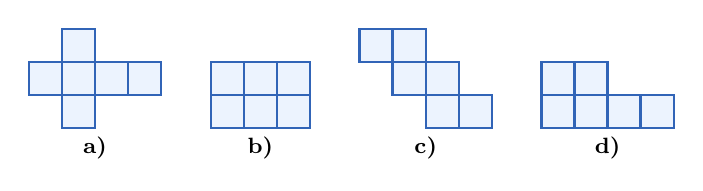
\begin{tikzpicture}[scale=0.42]
\foreach \x/\y in {1/2,0/1,1/1,2/1,3/1,1/0}{\draw[geo,fill=tmBlue!10] (\x,\y) rectangle ++(1,1);}
\node[lbl] at (2,-0.6){\pa{a}};
\begin{scope}[xshift=5.5cm]
\foreach \x/\y in {0/0,1/0,2/0,0/1,1/1,2/1}{\draw[geo,fill=tmBlue!10] (\x,\y) rectangle ++(1,1);}
\node[lbl] at (1.5,-0.6){\pa{b}};
\end{scope}
\begin{scope}[xshift=10cm]
\foreach \x/\y in {0/2,1/2,1/1,2/1,2/0,3/0}{\draw[geo,fill=tmBlue!10] (\x,\y) rectangle ++(1,1);}
\node[lbl] at (2,-0.6){\pa{c}};
\end{scope}
\begin{scope}[xshift=15.5cm]
\foreach \x/\y in {0/0,1/0,2/0,3/0,0/1,1/1}{\draw[geo,fill=tmBlue!10] (\x,\y) rectangle ++(1,1);}
\node[lbl] at (2,-0.6){\pa{d}};
\end{scope}
\end{tikzpicture}
\end{center}
\end{probbox}
\probsol{
\pa{a} Hàng $4$ hình vuông gấp thành $4$ mặt bên; hình vuông phía trên là nắp, hình vuông phía dưới là đáy. Đây là hình khai triển.\par
\pa{b} Gấp khối $2\times3$ hình vuông thì có các hình vuông chồng lên nhau và còn hở hai mặt. Không phải hình khai triển.\par
\pa{c} Hình ``bậc thang'' này gấp được thành hình lập phương, không có mặt nào chồng lên nhau. Đây là hình khai triển.\par
\pa{d} Hai hình vuông phía trên cùng gấp vào một mặt ở đầu hộp, còn đầu kia bị hở. Không phải hình khai triển.
\dapso{Hình \textbf{a)} và hình \textbf{c)}.}}
\gap
\begin{probbox}{3}{\relax}
Tính diện tích xung quanh và diện tích toàn phần của hình hộp chữ nhật có:
\begin{cols2}
\pa{a} $a=9$ cm, $b=6$ cm, $c=5$ cm; & \pa{b} $a=2{,}5$ m, $b=1{,}5$ m, $c=1{,}2$ m;\\
\pa{c} $a=\dfrac45$ m, $b=\dfrac12$ m, $c=\dfrac13$ m; & \pa{d} $a=1{,}2$ dm, $b=8$ cm, $c=5$ cm.
\end{cols2}
\end{probbox}
\probsol{
\pa{a} $S_{xq}=(9+6)\times2\times5=150$ cm$^2$; $S_{tp}=150+9\times6\times2=258$ cm$^2$.\par
\pa{b} $S_{xq}=(2{,}5+1{,}5)\times2\times1{,}2=9{,}6$ m$^2$; $S_{tp}=9{,}6+2{,}5\times1{,}5\times2=17{,}1$ m$^2$.\par
\pa{c} $S_{xq}=\left(\dfrac45+\dfrac12\right)\times2\times\dfrac13=\dfrac{13}{10}\times\dfrac23=\dfrac{13}{15}$ m$^2$;\par
$S_{tp}=\dfrac{13}{15}+\dfrac45\times\dfrac12\times2=\dfrac{13}{15}+\dfrac{12}{15}=\dfrac53$ m$^2$.\par
\pa{d} $1{,}2$ dm $=12$ cm. $S_{xq}=(12+8)\times2\times5=200$ cm$^2$; $S_{tp}=200+12\times8\times2=392$ cm$^2$.
\dapso{\pa{a} $150$ cm$^2$, $258$ cm$^2$;\par \pa{b} $9{,}6$ m$^2$, $17{,}1$ m$^2$;\par \pa{c} $\dfrac{13}{15}$ m$^2$, $\dfrac53$ m$^2$;\par \pa{d} $200$ cm$^2$, $392$ cm$^2$.}}
\gap
\begin{probbox}{4}{\relax}
Tính diện tích xung quanh và diện tích toàn phần của hình lập phương có cạnh:
\begin{cols3}
\pa{a} $6$ cm; & \pa{b} $2{,}5$ dm; & \pa{c} $\dfrac34$ m.
\end{cols3}
\end{probbox}
\probsol{
\pa{a} $S_{xq}=6\times6\times4=144$ cm$^2$; $S_{tp}=6\times6\times6=216$ cm$^2$.\par
\pa{b} $S_{xq}=2{,}5\times2{,}5\times4=25$ dm$^2$; $S_{tp}=2{,}5\times2{,}5\times6=37{,}5$ dm$^2$.\par
\pa{c} $S_{xq}=\dfrac34\times\dfrac34\times4=\dfrac94$ m$^2$; $S_{tp}=\dfrac34\times\dfrac34\times6=\dfrac{27}8$ m$^2$.
\dapso{\pa{a} $144$ cm$^2$, $216$ cm$^2$;\par \pa{b} $25$ dm$^2$, $37{,}5$ dm$^2$;\par \pa{c} $\dfrac94$ m$^2$, $\dfrac{27}8$ m$^2$.}}
\gap
\begin{probbox}{5}{\relax}
Một hình hộp chữ nhật có chiều dài $15$ cm, chiều rộng $10$ cm, chiều cao $8$ cm. Tính:
\begin{cols3}
\pa{a} chu vi mặt đáy; & \pa{b} diện tích xung quanh; & \pa{c} diện tích toàn phần.
\end{cols3}
\end{probbox}
\probsol{
\pa{a} $(15+10)\times2=50$ cm.\par
\pa{b} $50\times8=400$ cm$^2$.\par
\pa{c} $400+15\times10\times2=700$ cm$^2$.
\dapso{\pa{a} $50$ cm; \pa{b} $400$ cm$^2$; \pa{c} $700$ cm$^2$.}}
\gap
\begin{probbox}{6}{\relax}
Mai gói một hộp quà dạng hình hộp chữ nhật dài $24$ cm, rộng $16$ cm, cao $10$ cm, giấy gói phủ kín tất cả các mặt. Mai cần ít nhất bao nhiêu xăng-ti-mét vuông giấy gói?
\end{probbox}
\probsol{
Giấy phải phủ kín $6$ mặt, tức là bằng diện tích toàn phần.\par
$S_{xq}=(24+16)\times2\times10=800$ cm$^2$.\par
$S_{tp}=800+24\times16\times2=1\,568$ cm$^2$.
\dapso{$1\,568$ cm$^2$.}}
\gap
\begin{probbox}{7}{\relax}
Một cái hộp dạng hình hộp chữ nhật dài $40$ cm, rộng $25$ cm, cao $20$ cm. Lan dán giấy màu xanh vào bốn mặt xung quanh và giấy màu vàng vào hai mặt đáy (chỉ dán mặt ngoài). Hỏi diện tích giấy màu nào lớn hơn và lớn hơn bao nhiêu xăng-ti-mét vuông?
\end{probbox}
\probsol{
Diện tích giấy xanh (diện tích xung quanh): $(40+25)\times2\times20=2\,600$ cm$^2$.\par
Diện tích giấy vàng (hai mặt đáy): $40\times25\times2=2\,000$ cm$^2$.\par
Giấy xanh nhiều hơn: $2\,600-2\,000=600$ cm$^2$.
\dapso{Giấy xanh, lớn hơn $600$ cm$^2$.}}
\gap
\begin{probbox}{8}{\relax}
Một cái thùng bằng sắt không có nắp dạng hình hộp chữ nhật dài $60$ cm, rộng $40$ cm, cao $30$ cm. Tính diện tích sắt dùng để làm cái thùng đó (không tính mép hàn).
\end{probbox}
\probsol{
Diện tích xung quanh: $(60+40)\times2\times30=6\,000$ cm$^2$.\par
Diện tích đáy: $60\times40=2\,400$ cm$^2$.\par
Diện tích sắt: $6\,000+2\,400=8\,400$ cm$^2$.
\dapso{$8\,400$ cm$^2$.}}
\gap
\begin{probbox}{9}{\relax}
Một phòng học dạng hình hộp chữ nhật dài $8$ m, rộng $6$ m, cao $3{,}5$ m. Người ta quét vôi bốn bức tường và trần nhà; diện tích các cửa là $9{,}5$ m$^2$. Tính diện tích cần quét vôi.
\end{probbox}
\probsol{
Diện tích bốn bức tường: $(8+6)\times2\times3{,}5=98$ m$^2$.\par
Diện tích trần nhà: $8\times6=48$ m$^2$.\par
Diện tích cần quét vôi: $98+48-9{,}5=136{,}5$ m$^2$.
\dapso{$136{,}5$ m$^2$.}}
\gap
\begin{probbox}{10}{\relax}
Một bể nước dạng hình lập phương không có nắp, cạnh $1{,}5$ m. Người ta sơn mặt ngoài của bể (các mặt bên và đáy). Tính diện tích được sơn.
\end{probbox}
\probsol{
Diện tích một mặt: $1{,}5\times1{,}5=2{,}25$ m$^2$.\par
Bể không có nắp có $5$ mặt: $2{,}25\times5=11{,}25$ m$^2$.
\dapso{$11{,}25$ m$^2$.}}
\gap
\begin{probbox}{11}{\relax}
Một hình lập phương có diện tích xung quanh là $100$ cm$^2$. Tính độ dài cạnh và diện tích toàn phần của hình lập phương đó.
\end{probbox}
\probsol{
Diện tích một mặt: $100:4=25$ cm$^2$; vì $25=5\times5$ nên cạnh dài $5$ cm.\par
$S_{tp}=25\times6=150$ cm$^2$.
\dapso{$5$ cm; $150$ cm$^2$.}}
\gap
\begin{probbox}{12}{\relax}
Một hình lập phương có diện tích toàn phần là $600$ cm$^2$. Tính diện tích xung quanh của hình lập phương đó.
\end{probbox}
\probsol{
Diện tích một mặt: $600:6=100$ cm$^2$.\par
$S_{xq}=100\times4=400$ cm$^2$.
\dapso{$400$ cm$^2$.}}
\gap
\begin{probbox}{13}{\relax}
Một hình lập phương có diện tích xung quanh là $1{,}44$ m$^2$. Tính độ dài cạnh và diện tích toàn phần của hình lập phương đó.
\end{probbox}
\probsol{
Diện tích một mặt: $1{,}44:4=0{,}36$ m$^2$; vì $0{,}36=0{,}6\times0{,}6$ nên cạnh dài $0{,}6$ m.\par
$S_{tp}=0{,}36\times6=2{,}16$ m$^2$.
\dapso{$0{,}6$ m; $2{,}16$ m$^2$.}}
\gap
\begin{probbox}{14}{\relax}
Một hình hộp chữ nhật có diện tích xung quanh là $360$ cm$^2$, chiều cao $9$ cm. Chiều dài hơn chiều rộng $4$ cm. Tính chiều dài và chiều rộng của hình hộp.
\end{probbox}
\probsol{
Chu vi mặt đáy: $360:9=40$ cm.\par
Nửa chu vi (dài $+$ rộng): $40:2=20$ cm.\par
Chiều dài: $(20+4):2=12$ cm.\quad Chiều rộng: $20-12=8$ cm.
\dapso{Chiều dài $12$ cm, chiều rộng $8$ cm.}}
\gap
\begin{probbox}{15}{\relax}
Một hình hộp chữ nhật có chu vi đáy $36$ dm, chiều cao $7$ dm. Tính diện tích xung quanh của hình hộp đó.
\end{probbox}
\probsol{
$S_{xq}=36\times7=252$ dm$^2$.
\dapso{$252$ dm$^2$.}}
\gap
\begin{probbox}{16}{\relax}
Một hình hộp chữ nhật có diện tích xung quanh $480$ cm$^2$, chu vi đáy $48$ cm. Tính chiều cao của hình hộp.
\end{probbox}
\probsol{
Chiều cao $=$ diện tích xung quanh $:$ chu vi đáy.\par
$c=480:48=10$ cm.
\dapso{$10$ cm.}}
\gap
\begin{probbox}{17}{\relax}
Một hình hộp chữ nhật có chiều dài $2{,}4$ m, chiều rộng $1{,}6$ m và diện tích toàn phần $19{,}68$ m$^2$. Tính chiều cao của hình hộp.
\end{probbox}
\probsol{
Diện tích hai đáy: $2{,}4\times1{,}6\times2=7{,}68$ m$^2$.\par
Diện tích xung quanh: $19{,}68-7{,}68=12$ m$^2$.\par
Chu vi đáy: $(2{,}4+1{,}6)\times2=8$ m.\par
Chiều cao: $12:8=1{,}5$ m.
\dapso{$1{,}5$ m.}}
\gap
\begin{probbox}{18}{\relax}
Một cái thùng gỗ dạng hình hộp chữ nhật dài $1{,}2$ m, rộng $0{,}8$ m, cao $0{,}6$ m. Người ta quét vecni toàn bộ mặt ngoài của thùng, mỗi mét vuông hết $0{,}25$ kg vecni. Hỏi cần bao nhiêu ki-lô-gam vecni?
\end{probbox}
\probsol{
$S_{xq}=(1{,}2+0{,}8)\times2\times0{,}6=2{,}4$ m$^2$.\par
$S_{tp}=2{,}4+1{,}2\times0{,}8\times2=4{,}32$ m$^2$.\par
Số vecni cần dùng: $0{,}25\times4{,}32=1{,}08$ kg.
\dapso{$1{,}08$ kg.}}
\gap
\begin{probbox}{19}{\relax}
Một bể bơi dạng hình hộp chữ nhật dài $25$ m, rộng $10$ m, sâu $1{,}6$ m. Người ta lát kín đáy và xung quanh thành bể bằng các viên gạch hình chữ nhật kích thước $25$ cm và $20$ cm. Hỏi cần bao nhiêu viên gạch? (Coi diện tích mạch vữa không đáng kể.)
\end{probbox}
\probsol{
Diện tích xung quanh: $(25+10)\times2\times1{,}6=112$ m$^2$.\quad Diện tích đáy: $25\times10=250$ m$^2$.\par
Diện tích cần lát: $112+250=362$ m$^2$.\par
Diện tích một viên gạch: $25\times20=500$ cm$^2$ $=0{,}05$ m$^2$.\par
Số viên gạch: $362:0{,}05=7\,240$ viên.
\dapso{$7\,240$ viên gạch.}}
\gap
\begin{probbox}{20}{\relax}
Một cái ao nuôi cá dạng hình hộp chữ nhật dài $3$ m, rộng $2$ m, sâu $0{,}8$ m. Người ta lát đáy và xung quanh thành ao bằng gạch hình vuông cạnh $2$ dm. Hỏi cần bao nhiêu viên gạch?
\end{probbox}
\probsol{
Diện tích xung quanh: $(3+2)\times2\times0{,}8=8$ m$^2$.\quad Diện tích đáy: $3\times2=6$ m$^2$.\par
Diện tích cần lát: $8+6=14$ m$^2$ $=1\,400$ dm$^2$.\par
Một viên gạch: $2\times2=4$ dm$^2$.\quad Số viên gạch: $1\,400:4=350$ viên.
\dapso{$350$ viên gạch.}}
\gap
\begin{probbox}{21}{\relax}
Một hình hộp chữ nhật có chu vi đáy $30$ cm; chiều dài hơn chiều rộng $3$ cm, chiều cao bằng $\dfrac23$ chiều dài. Tính diện tích xung quanh và diện tích toàn phần của hình hộp.
\end{probbox}
\probsol{
Nửa chu vi đáy: $30:2=15$ cm.\par
Chiều dài: $(15+3):2=9$ cm.\quad Chiều rộng: $6$ cm.\quad Chiều cao: $9\times\dfrac23=6$ cm.\par
$S_{xq}=30\times6=180$ cm$^2$.\par
$S_{tp}=180+9\times6\times2=288$ cm$^2$.
\dapso{$180$ cm$^2$; $288$ cm$^2$.}}
\gap
\begin{probbox}{22}{\relax}
So sánh diện tích toàn phần của hình lập phương cạnh $6$ cm với diện tích toàn phần của hình hộp chữ nhật dài $8$ cm, rộng $6$ cm, cao $4$ cm.
\end{probbox}
\probsol{
Hình lập phương: $6\times6\times6=216$ cm$^2$.\par
Hình hộp chữ nhật: $(8+6)\times2\times4+8\times6\times2=112+96=208$ cm$^2$.\par
$216-208=8$ cm$^2$.
\dapso{Diện tích toàn phần của hình lập phương lớn hơn, lớn hơn $8$ cm$^2$.}}
\gap
\begin{probbox}{23}{\relax}
Một hình hộp chữ nhật có đáy là hình vuông cạnh $5$ cm, chiều cao $12$ cm. Tính diện tích xung quanh và diện tích toàn phần của hình hộp.
\end{probbox}
\probsol{
Chu vi đáy: $5\times4=20$ cm.\par
$S_{xq}=20\times12=240$ cm$^2$.\par
$S_{tp}=240+5\times5\times2=290$ cm$^2$.
\dapso{$240$ cm$^2$; $290$ cm$^2$.}}
\gap
\begin{probbox}{24}{\relax}
Khung một chiếc đèn lồng có dạng hình hộp chữ nhật, đáy là hình vuông cạnh $20$ cm, chiều cao $35$ cm. Người ta dán giấy kín bốn mặt xung quanh và mặt đáy. Hỏi đã dùng bao nhiêu đề-xi-mét vuông giấy?
\end{probbox}
\probsol{
Bốn mặt xung quanh: $20\times4\times35=2\,800$ cm$^2$.\par
Mặt đáy: $20\times20=400$ cm$^2$.\par
Diện tích giấy: $2\,800+400=3\,200$ cm$^2$ $=32$ dm$^2$.
\dapso{$32$ dm$^2$.}}
\gap
\begin{probbox}{25}{\relax}
Người ta dùng một miếng bìa vừa đủ để làm một cái hộp không có nắp dạng hình lập phương cạnh $2{,}5$ dm. Tính diện tích miếng bìa đó (không tính mép dán).
\end{probbox}
\probsol{
Diện tích một mặt: $2{,}5\times2{,}5=6{,}25$ dm$^2$.\par
Hộp có $5$ mặt: $6{,}25\times5=31{,}25$ dm$^2$.
\dapso{$31{,}25$ dm$^2$.}}
\gap
\begin{probbox}{26}{\relax}
Một cái thùng không có nắp dạng hình lập phương có chu vi đáy $4{,}8$ m. Người ta sơn cả mặt trong và mặt ngoài của thùng, cứ $3$ m$^2$ hết $1$ kg sơn. Hỏi cần bao nhiêu ki-lô-gam sơn?
\end{probbox}
\probsol{
Cạnh thùng: $4{,}8:4=1{,}2$ m.\quad Diện tích một mặt: $1{,}2\times1{,}2=1{,}44$ m$^2$.\par
Thùng không nắp có $5$ mặt, sơn cả hai phía: $1{,}44\times5\times2=14{,}4$ m$^2$.\par
Số sơn cần dùng: $14{,}4:3=4{,}8$ kg.
\dapso{$4{,}8$ kg.}}
\gap
\begin{probbox}{27}{\relax}
Tổng độ dài $12$ cạnh của một hình hộp chữ nhật là $96$ cm. Chiều dài $12$ cm, chiều rộng $8$ cm. Tính diện tích toàn phần của hình hộp.
\end{probbox}
\probsol{
Hình hộp chữ nhật có $4$ cạnh dài, $4$ cạnh rộng và $4$ cạnh cao.\par
Dài $+$ rộng $+$ cao: $96:4=24$ cm.\quad Chiều cao: $24-12-8=4$ cm.\par
$S_{xq}=(12+8)\times2\times4=160$ cm$^2$.\par
$S_{tp}=160+12\times8\times2=352$ cm$^2$.
\dapso{$352$ cm$^2$.}}
\gap
\begin{probbox}{28}{\relax}
Tổng độ dài $12$ cạnh của một hình lập phương là $72$ cm. Tính diện tích toàn phần của hình lập phương đó.
\end{probbox}
\probsol{
Cạnh: $72:12=6$ cm.\par
$S_{tp}=6\times6\times6=216$ cm$^2$.
\dapso{$216$ cm$^2$.}}
\gap
\begin{probbox}{29}{\relax}
Một bể cá bằng kính không có nắp dạng hình hộp chữ nhật dài $80$ cm, rộng $40$ cm, cao $50$ cm. Hỏi đã dùng bao nhiêu đề-xi-mét vuông kính?
\end{probbox}
\probsol{
Bốn mặt xung quanh: $(80+40)\times2\times50=12\,000$ cm$^2$.\par
Mặt đáy: $80\times40=3\,200$ cm$^2$.\par
Diện tích kính: $12\,000+3\,200=15\,200$ cm$^2$ $=152$ dm$^2$.
\dapso{$152$ dm$^2$.}}
\gap
\begin{probbox}{30}{\relax}
Diện tích toàn phần của một hình lập phương lớn hơn diện tích xung quanh của nó $50$ cm$^2$. Tính diện tích xung quanh của hình lập phương đó.
\end{probbox}
\probsol{
Phần hơn chính là diện tích hai mặt đáy: một mặt là $50:2=25$ cm$^2$.\par
$S_{xq}=25\times4=100$ cm$^2$.
\dapso{$100$ cm$^2$.}}
\dividerbar{Thử thách -- Nâng cao}
\begin{probbox}{31}{\stars{1}}
Một hình hộp chữ nhật có diện tích mặt đáy $120$ cm$^2$. Chiều dài hơn chiều cao $9$ cm, chiều cao bằng $\dfrac25$ chiều dài. Tính diện tích xung quanh và diện tích toàn phần của hình hộp.
\end{probbox}
\probsol{
Chiều cao $2$ phần, chiều dài $5$ phần; hiệu là $3$ phần $=9$ cm nên $1$ phần là $3$ cm.\par
Chiều cao: $3\times2=6$ cm.\quad Chiều dài: $3\times5=15$ cm.\quad Chiều rộng: $120:15=8$ cm.\par
$S_{xq}=(15+8)\times2\times6=276$ cm$^2$.\par
$S_{tp}=276+120\times2=516$ cm$^2$.
\dapso{$276$ cm$^2$; $516$ cm$^2$.}}
\gap
\begin{probbox}{32}{\stars{1}}
Một bể nước dạng hình hộp chữ nhật có diện tích xung quanh $10{,}5$ m$^2$, chiều cao $1{,}5$ m. Chiều dài hơn chiều rộng $1$ m. Tính chiều dài và chiều rộng của bể.
\end{probbox}
\probsol{
Chu vi đáy: $10{,}5:1{,}5=7$ m.\quad Nửa chu vi: $7:2=3{,}5$ m.\par
Chiều dài: $(3{,}5+1):2=2{,}25$ m.\quad Chiều rộng: $3{,}5-2{,}25=1{,}25$ m.
\dapso{Chiều dài $2{,}25$ m, chiều rộng $1{,}25$ m.}}
\gap
\begin{probbox}{33}{\stars{1}}
Một cái thùng sắt dạng hình hộp chữ nhật có chiều rộng bằng $\dfrac34$ chiều dài và kém chiều dài $0{,}5$ m; chiều cao $1{,}2$ m.\par
\pa{a} Tính diện tích toàn phần của thùng.\par
\pa{b} Người ta sơn kín mặt ngoài của thùng, cứ $4$ m$^2$ hết $3$ kg sơn. Hỏi cần bao nhiêu ki-lô-gam sơn?
\end{probbox}
\probsol{
\pa{a} Chiều dài $4$ phần, chiều rộng $3$ phần; hiệu là $1$ phần $=0{,}5$ m.\par
Chiều dài: $0{,}5\times4=2$ m.\quad Chiều rộng: $0{,}5\times3=1{,}5$ m.\par
$S_{xq}=(2+1{,}5)\times2\times1{,}2=8{,}4$ m$^2$.\quad $S_{tp}=8{,}4+2\times1{,}5\times2=14{,}4$ m$^2$.\par
\pa{b} Mỗi mét vuông hết $3:4=0{,}75$ kg. Số sơn: $0{,}75\times14{,}4=10{,}8$ kg.
\dapso{\pa{a} $14{,}4$ m$^2$; \pa{b} $10{,}8$ kg.}}
\gap
\begin{probbox}{34}{\stars{2}}
Nếu tăng cạnh của một hình lập phương thêm $2$ cm thì diện tích toàn phần tăng thêm $120$ cm$^2$. Tính cạnh của hình lập phương ban đầu.
\end{probbox}
\probsol{
Mỗi mặt trong $6$ mặt tăng thêm $120:6=20$ cm$^2$.\par
Hình vuông cạnh $a$ thành hình vuông cạnh $a+2$: phần tăng thêm gồm hai dải hình chữ nhật $a$ và $2$, cùng một hình vuông nhỏ $2$ và $2$ ở góc.\par
$a\times2\times2+2\times2=20$, nên $a\times4=16$ và $a=4$ cm.\par
\emph{Thử lại:} $6\times6\times6-4\times4\times6=216-96=120$ cm$^2$.
\dapso{$4$ cm.}}
\gap
\begin{probbox}{35}{\stars{1}}
Người ta ghép hai hình lập phương cạnh $5$ cm, áp sát một mặt vào nhau, được một hình hộp chữ nhật. Tính diện tích toàn phần của hình hộp chữ nhật đó. Diện tích này ít hơn tổng diện tích toàn phần của hai hình lập phương bao nhiêu?
\end{probbox}
\probsol{
Hình hộp chữ nhật có kích thước $10$ cm, $5$ cm, $5$ cm.\par
$S_{tp}=(10+5)\times2\times5+10\times5\times2=150+100=250$ cm$^2$.\par
Hai hình lập phương: $5\times5\times6\times2=300$ cm$^2$.\par
Ít hơn $300-250=50$ cm$^2$: hai mặt áp vào nhau ($2\times25$ cm$^2$) bị che khuất.
\dapso{$250$ cm$^2$; ít hơn $50$ cm$^2$.}}
\gap
\begin{probbox}{36}{\stars{1}}
Xếp ba hình lập phương cạnh $4$ cm thành một hàng rồi dán lại được một hình hộp chữ nhật. Tính diện tích toàn phần của hình hộp chữ nhật đó.
\end{probbox}
\probsol{
Hình hộp chữ nhật có kích thước $12$ cm, $4$ cm, $4$ cm.\par
$S_{tp}=(12+4)\times2\times4+12\times4\times2=128+96=224$ cm$^2$.\par
\emph{Cách khác:} $3$ hình lập phương có $18$ mặt; mỗi chỗ ghép trong $2$ chỗ ghép che mất $2$ mặt, còn $18-4=14$ mặt: $14\times4\times4=224$ cm$^2$.
\dapso{$224$ cm$^2$.}}
\gap
\begin{probbox}{37}{\stars{1}}
Một hình hộp chữ nhật dài $10$ cm, rộng $6$ cm, cao $4$ cm được cắt thành hai phần bằng nhau bởi một nhát cắt song song với mặt đáy. Tính diện tích toàn phần của hình hộp ban đầu và tổng diện tích toàn phần của hai phần.
\end{probbox}
\probsol{
Ban đầu: $(10+6)\times2\times4+10\times6\times2=128+120=248$ cm$^2$.\par
Nhát cắt tạo thêm hai mặt mới, mỗi mặt $10\times6=60$ cm$^2$.\par
Tổng của hai phần: $248+60\times2=368$ cm$^2$.
\dapso{$248$ cm$^2$; $368$ cm$^2$.}}
\gap
\begin{probbox}{38}{\stars{1}}
Một hình hộp chữ nhật có đáy là hình vuông và diện tích xung quanh $160$ cm$^2$. Chiều cao gấp $2{,}5$ lần cạnh đáy. Tính diện tích toàn phần của hình hộp.
\end{probbox}
\probsol{
Mỗi mặt bên là hình chữ nhật có hai cạnh là cạnh đáy và $2{,}5$ lần cạnh đáy, nên bằng $2{,}5$ lần diện tích mặt đáy.\par
Diện tích xung quanh $=4\times2{,}5=10$ lần diện tích mặt đáy: một mặt đáy là $160:10=16$ cm$^2$ (cạnh đáy $4$ cm, chiều cao $10$ cm).\par
$S_{tp}=160+16\times2=192$ cm$^2$.
\dapso{$192$ cm$^2$.}}
\gap
\begin{probbox}{39}{\stars{1}}
Một hình lập phương có diện tích toàn phần $1{,}5$ m$^2$. Tính cạnh và diện tích xung quanh của hình lập phương đó.
\end{probbox}
\probsol{
Diện tích một mặt: $1{,}5:6=0{,}25$ m$^2$; vì $0{,}25=0{,}5\times0{,}5$ nên cạnh dài $0{,}5$ m.\par
$S_{xq}=0{,}25\times4=1$ m$^2$.
\dapso{$0{,}5$ m; $1$ m$^2$.}}
\gap
\begin{probbox}{40}{\stars{2}}
\begin{minipage}[t]{0.6\linewidth}
Từ một tấm bìa hình chữ nhật $40$ cm $\times\,30$ cm, Nam cắt ở mỗi góc một hình vuông cạnh $5$ cm rồi gấp các mép lên để được một cái hộp không nắp. Tính chiều dài, chiều rộng, chiều cao của hộp và diện tích bìa đã dùng làm hộp.
\end{minipage}\hfill
\begin{minipage}[t]{0.36\linewidth}\vspace{0pt}\centering
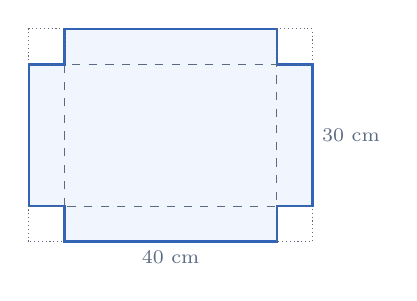
\begin{tikzpicture}[scale=0.09]
\draw[geo,fill=tmBlue!8] (5,0)--(35,0)--(35,5)--(40,5)--(40,25)--(35,25)--(35,30)--(5,30)--(5,25)--(0,25)--(0,5)--(5,5)--cycle;
\draw[dashed,Slate] (5,5) rectangle (35,25);
\foreach \x/\y in {0/0,35/0,0/25,35/25}{\draw[Slate,densely dotted] (\x,\y) rectangle ++(5,5);}
\node[dim,below] at (20,0){$40$ cm}; \node[dim,right] at (40,15){$30$ cm};
\end{tikzpicture}
\end{minipage}
\end{probbox}
\probsol{
Chiều dài: $40-5\times2=30$ cm.\quad Chiều rộng: $30-5\times2=20$ cm.\quad Chiều cao: $5$ cm.\par
Diện tích bìa đã dùng: $40\times30-5\times5\times4=1\,200-100=1\,100$ cm$^2$.\par
\emph{Thử lại:} $S_{xq}+$ đáy $=(30+20)\times2\times5+30\times20=500+600=1\,100$ cm$^2$.
\dapso{$30$ cm, $20$ cm, $5$ cm; $1\,100$ cm$^2$.}}
\gap
\begin{probbox}{41}{\stars{1}}
Một căn phòng dạng hình hộp chữ nhật dài $5$ m, rộng $4$ m, cao $3$ m. Người ta sơn mặt trong các bức tường và trần nhà. Diện tích các cửa là $4$ m$^2$. Tiền công sơn là $25\,000$ đồng mỗi mét vuông. Tính số tiền công phải trả.
\end{probbox}
\probsol{
Bốn bức tường: $(5+4)\times2\times3=54$ m$^2$.\quad Trần nhà: $5\times4=20$ m$^2$.\par
Diện tích cần sơn: $54+20-4=70$ m$^2$.\par
Tiền công: $25\,000\times70=1\,750\,000$ đồng.
\dapso{$1\,750\,000$ đồng.}}
\gap
\begin{probbox}{42}{\stars{1}}
Tổng độ dài $12$ cạnh của một hình hộp chữ nhật là $120$ cm. Chiều dài gấp $3$ lần chiều rộng, chiều cao gấp $2$ lần chiều rộng. Tính diện tích toàn phần của hình hộp.
\end{probbox}
\probsol{
Dài $+$ rộng $+$ cao: $120:4=30$ cm, bằng $3+1+2=6$ lần chiều rộng.\par
Chiều rộng: $30:6=5$ cm.\quad Chiều dài: $15$ cm.\quad Chiều cao: $10$ cm.\par
$S_{tp}=(15+5)\times2\times10+15\times5\times2=400+150=550$ cm$^2$.
\dapso{$550$ cm$^2$.}}
\gap
\begin{probbox}{43}{\stars{2}}
Ba mặt khác nhau của một hình hộp chữ nhật có diện tích $12$ cm$^2$, $15$ cm$^2$ và $20$ cm$^2$. Tính diện tích toàn phần của hình hộp và tìm ba kích thước của nó (là số tự nhiên, đơn vị xăng-ti-mét).
\end{probbox}
\probsol{
Mỗi mặt xuất hiện hai lần: $S_{tp}=(12+15+20)\times2=94$ cm$^2$.\par
Thử các số tự nhiên: cạnh chung của hai mặt $12$ cm$^2$ và $15$ cm$^2$ chia hết cả $12$ và $15$, nên là $1$ hoặc $3$.\par
Nếu là $3$: hai cạnh còn lại là $12:3=4$ và $15:3=5$, và $4\times5=20$. \checkmark\par
(Nếu là $1$: $12\times15=180\neq20$.)
\dapso{$94$ cm$^2$; $3$ cm, $4$ cm, $5$ cm.}}
\gap
\begin{probbox}{44}{\stars{1}}
Một cái hộp không nắp dạng hình lập phương cạnh $15$ cm. Người ta dán giấy màu cả mặt trong và mặt ngoài của hộp. Tính diện tích giấy màu đã dùng.
\end{probbox}
\probsol{
Diện tích một mặt: $15\times15=225$ cm$^2$.\par
$5$ mặt, dán cả hai phía: $225\times5\times2=2\,250$ cm$^2$.
\dapso{$2\,250$ cm$^2$.}}
\gap
\begin{probbox}{45}{\stars{1}}
Một hình hộp chữ nhật có đáy là hình vuông cạnh $6$ cm. Diện tích xung quanh gấp $3$ lần tổng diện tích hai đáy. Tính chiều cao và diện tích toàn phần của hình hộp.
\end{probbox}
\probsol{
Diện tích hai đáy: $6\times6\times2=72$ cm$^2$.\par
$S_{xq}=72\times3=216$ cm$^2$.\quad Chiều cao: $216:(6\times4)=9$ cm.\par
$S_{tp}=216+72=288$ cm$^2$.
\dapso{$9$ cm; $288$ cm$^2$.}}
\gap
\begin{probbox}{46}{\stars{1}}
Hai hình hộp chữ nhật giống nhau, mỗi hình có kích thước $8$ cm, $5$ cm, $3$ cm, được dán áp sát vào nhau theo mặt lớn nhất. Tính diện tích toàn phần của hình hộp chữ nhật mới.
\end{probbox}
\probsol{
Mặt lớn nhất là $8\times5=40$ cm$^2$. Hình hộp mới có kích thước $8$ cm, $5$ cm, $6$ cm.\par
$S_{tp}=(8+5)\times2\times6+8\times5\times2=156+80=236$ cm$^2$.\par
\emph{Thử lại:} một hình hộp có $(8+5)\times2\times3+80=158$ cm$^2$; $158\times2-40\times2=236$ cm$^2$.
\dapso{$236$ cm$^2$.}}
\gap
\begin{probbox}{47}{\stars{2}}
Một bể bơi dạng hình hộp chữ nhật dài $12{,}5$ m, rộng $6$ m, sâu $1{,}4$ m. Người ta lát đáy và xung quanh thành bể bằng gạch kích thước $25$ cm $\times\,20$ cm. Gạch được bán theo hộp, mỗi hộp $12$ viên. Hỏi phải mua bao nhiêu hộp gạch?
\end{probbox}
\probsol{
Xung quanh: $(12{,}5+6)\times2\times1{,}4=51{,}8$ m$^2$.\quad Đáy: $12{,}5\times6=75$ m$^2$.\par
Diện tích cần lát: $51{,}8+75=126{,}8$ m$^2$.\quad Một viên gạch: $0{,}05$ m$^2$.\par
Số viên gạch: $126{,}8:0{,}05=2\,536$ viên.\par
$2\,536:12=211$ (dư $4$), nên $211$ hộp chưa đủ; phải mua $212$ hộp.
\dapso{$212$ hộp.}}
\gap
\begin{probbox}{48}{\stars{1}}
Một hình lập phương có diện tích toàn phần bằng diện tích toàn phần của hình hộp chữ nhật dài $12$ cm, rộng $9$ cm, cao $4$ cm. Tính cạnh của hình lập phương.
\end{probbox}
\probsol{
Hình hộp chữ nhật: $(12+9)\times2\times4+12\times9\times2=168+216=384$ cm$^2$.\par
Một mặt của hình lập phương: $384:6=64$ cm$^2$ $=8\times8$.
\dapso{$8$ cm.}}
\gap
\begin{probbox}{49}{\stars{2}}
Một hình hộp chữ nhật cao $5$ cm. Nếu giảm chiều dài $3$ cm và tăng chiều rộng $3$ cm thì mặt đáy trở thành hình vuông cạnh $8$ cm. So sánh diện tích toàn phần của hình hộp cũ và hình hộp mới.
\end{probbox}
\probsol{
Chiều dài cũ: $8+3=11$ cm.\quad Chiều rộng cũ: $8-3=5$ cm.\par
Chu vi đáy không đổi ($32$ cm) nên diện tích xung quanh không đổi: $32\times5=160$ cm$^2$.\par
Hình cũ: $160+11\times5\times2=270$ cm$^2$.\quad Hình mới: $160+8\times8\times2=288$ cm$^2$.\par
Hình mới lớn hơn $18$ cm$^2$.
\dapso{Diện tích toàn phần của hình hộp mới lớn hơn, lớn hơn $18$ cm$^2$.}}
\gap
\begin{probbox}{50}{\stars{2}}
Một hình lập phương cạnh $6$ cm được cắt thành $8$ hình lập phương nhỏ bằng nhau. Tính tổng diện tích toàn phần của $8$ hình lập phương nhỏ và so sánh với diện tích toàn phần của hình lập phương lớn.
\end{probbox}
\probsol{
Mỗi hình lập phương nhỏ có cạnh $6:2=3$ cm.\par
Một hình nhỏ: $3\times3\times6=54$ cm$^2$.\quad $8$ hình: $54\times8=432$ cm$^2$.\par
Hình lớn: $6\times6\times6=216$ cm$^2$.\quad $432:216=2$.
\dapso{$432$ cm$^2$, gấp $2$ lần.}}
\clearpage
\titlehead
\begingroup\setbox0=\vbox{\section*{Thể tích}}\endgroup
\chapterhead{4}{Thể tích}
\shead{Thể tích và đơn vị đo thể tích}
\gdef\cuboidVT#1#2#3#4{\coordinate (Q) at (0,0); \coordinate (P) at (#1,0); \coordinate (C) at (#1,#3); \coordinate (D) at (0,#3);
 \coordinate (M) at ({0.5*#2},{0.38*#2}); \coordinate (N) at ($(P)+(M)$); \coordinate (B) at ($(C)+(M)$); \coordinate (A) at ($(D)+(M)$);
 \fill[tmBlue!6] (Q)--(P)--(C)--(D)--cycle; \fill[tmBlue!3] (D)--(C)--(B)--(A)--cycle; \fill[tmBlue!13] (P)--(N)--(B)--(C)--cycle;
 \ifdim #4pt>0pt \coordinate (wl) at (0,#4);
  \fill[cyan!30] (Q)--(P)--($(P)+(wl)$)--($(Q)+(wl)$)--cycle; \fill[cyan!45] (P)--(N)--($(N)+(wl)$)--($(P)+(wl)$)--cycle;
  \fill[cyan!16] ($(Q)+(wl)$)--($(P)+(wl)$)--($(N)+(wl)$)--($(M)+(wl)$)--cycle;
  \draw[cyan!60!black,line width=0.5pt] ($(Q)+(wl)$)--($(P)+(wl)$)--($(N)+(wl)$);
  \draw[cyan!60!black,line width=0.4pt,dashed] ($(N)+(wl)$)--($(M)+(wl)$)--($(Q)+(wl)$); \fi
 \draw[geo,dashed,line width=0.6pt] (M)--(Q) (M)--(N) (M)--(A);
 \draw[geo] (Q)--(P)--(C)--(D)--cycle (D)--(A)--(B)--(C) (P)--(N)--(B);}
\begin{knowbox}
\begin{minipage}[t]{0.6\linewidth}
\textbf{Thể tích} của một hình là độ lớn phần không gian mà hình đó chiếm chỗ. Để đo thể tích, ta đếm xem hình đó chứa bao nhiêu \emph{hình lập phương đơn vị}.\par
\smallskip
\textbf{Xăng-ti-mét khối} (cm$^3$) là thể tích của hình lập phương có cạnh dài $1$ cm. Tương tự, $1$ dm$^3$ là thể tích hình lập phương cạnh $1$ dm, $1$ m$^3$ là thể tích hình lập phương cạnh $1$ m.
\[1\text{ m}^3=1\,000\text{ dm}^3\qquad 1\text{ dm}^3=1\,000\text{ cm}^3\]
Mỗi đơn vị đo thể tích gấp $1\,000$ lần đơn vị bé hơn tiếp liền, nên khi đổi đơn vị ta dời dấu phẩy \textbf{ba} chữ số.\par
\smallskip
Với chất lỏng:\[1\text{ l}=1\text{ dm}^3\qquad 1\text{ ml}=1\text{ cm}^3\qquad 1\text{ m}^3=1\,000\text{ l}\]\vspace{-\baselineskip}
\end{minipage}\hfill
\begin{minipage}[t]{0.36\linewidth}\vspace{6pt}\centering
\begin{tikzpicture}[scale=0.62]
\cuboidVT{3}{3}{3}{0}
\foreach \i in {1,2}{\draw[tmBlue!60,line width=0.35pt] (\i,0)--(\i,3)--++(1.5,1.14) (0,\i)--(3,\i)--++(1.5,1.14)
 ($(0,3)+\i*(0.5,0.38)$)--++(3,0)--++(0,-3);}
\draw[geo] (Q)--(P)--(C)--(D)--cycle (D)--(A)--(B)--(C) (P)--(N)--(B);
\node[dim,below] at ($(Q)!0.5!(P)$){$1$ dm $=10$ cm};
\end{tikzpicture}\par\smallskip
{\scriptsize\color{Slate} $1$ dm$^3$: $10$ lớp, mỗi lớp $10\times10$ hình lập phương $1$ cm$^3$, tức là $1\,000$ cm$^3$ (hình vẽ thu gọn)}
\end{minipage}
\end{knowbox}
\shead{Thể tích hình hộp chữ nhật, hình lập phương}
\begin{knowbox}
\begin{minipage}[t]{0.6\linewidth}
Hình hộp chữ nhật dài $5$ cm, rộng $3$ cm, cao $2$ cm xếp được $2$ lớp, mỗi lớp $5\times3=15$ hình lập phương $1$ cm$^3$, tức là $5\times3\times2=30$ cm$^3$.\par
\smallskip
Muốn tính \textbf{thể tích hình hộp chữ nhật}, ta lấy chiều dài nhân với chiều rộng rồi nhân với chiều cao (cùng một đơn vị đo):
\[V=a\times b\times c=S_{\text{đáy}}\times c\]
\textbf{Thể tích hình lập phương} cạnh $a$: \quad $V=a\times a\times a$.\par
\smallskip
Tính ngược lại: \quad $c=V:(a\times b)$, \quad $S_{\text{đáy}}=V:c$.
\end{minipage}\hfill
\begin{minipage}[t]{0.36\linewidth}\vspace{6pt}\centering
\begin{tikzpicture}[scale=0.55]
\cuboidVT{5}{3}{2}{0}
\foreach \i in {1,...,4}{\draw[tmBlue!60,line width=0.35pt] (\i,0)--(\i,2)--++(1.5,1.14);}
\draw[tmBlue!60,line width=0.35pt] (0,1)--(5,1)--++(1.5,1.14);
\foreach \k in {1,2}{\draw[tmBlue!60,line width=0.35pt] ($(0,2)+\k*(0.5,0.38)$)--++(5,0)--++(0,-2);}
\draw[geo] (Q)--(P)--(C)--(D)--cycle (D)--(A)--(B)--(C) (P)--(N)--(B);
\node[dim,below] at ($(Q)!0.5!(P)$){$5$ cm}; \node[dim,right] at ($(P)!0.5!(N)$){$3$ cm}; \node[dim,left] at ($(Q)!0.5!(D)$){$2$ cm};
\end{tikzpicture}
\end{minipage}
\end{knowbox}
\needspace{8\baselineskip}
\shead{Thể tích vật chìm trong nước}
\begin{knowbox}
Hòn đá, cây san hô có hình dạng không xác định nên không tính thể tích bằng công thức được. Thả vật vào bể nước sao cho vật \textbf{ngập hoàn toàn} trong nước: mực nước dâng lên vì vật đã chiếm một phần thể tích của bể.
\begin{itemize}[leftmargin=1.2em,itemsep=1pt,topsep=2pt]
\item \emph{Cách 1:} thể tích vật $=$ thể tích (nước $+$ vật) $-$ thể tích nước.
\item \emph{Cách 2:} thể tích vật $=$ diện tích đáy bể $\times$ chiều cao phần nước dâng lên.
\end{itemize}
Nếu bể đã đầy nước thì thể tích nước \textbf{tràn ra} bằng thể tích của vật.
\end{knowbox}
\gap
\begin{exbox}{\ExWord\ 1}
Viết số thích hợp vào chỗ chấm.
\begin{cols2}
\pa{a} $3{,}5$ m$^3=\ldots$ dm$^3$ & \pa{b} $2\,400$ cm$^3=\ldots$ dm$^3$\\
\pa{c} $0{,}75$ dm$^3=\ldots$ cm$^3=\ldots$ ml & \pa{d} $1{,}2$ m$^3=\ldots$ l
\end{cols2}
\guide
\pa{a} $1$ m$^3=1\,000$ dm$^3$ nên $3{,}5$ m$^3=3{,}5\times1\,000=3\,500$ dm$^3$.\par
\pa{b} $2\,400$ cm$^3=2\,400:1\,000=2{,}4$ dm$^3$.\par
\pa{c} $0{,}75$ dm$^3=750$ cm$^3=750$ ml.\par
\pa{d} $1{,}2$ m$^3=1\,200$ dm$^3=1\,200$ l.
\dapso{\pa{a} $3\,500$; \pa{b} $2{,}4$; \pa{c} $750$; $750$; \pa{d} $1\,200$.}
\end{exbox}
\gap
\begin{exbox}{\ExWord\ 2}
Tính thể tích của:\par
\pa{a} hình hộp chữ nhật có chiều dài $1{,}2$ m, chiều rộng $5$ dm, chiều cao $8$ dm;\par
\pa{b} hình lập phương có cạnh $2{,}5$ cm.
\guide
\pa{a} Đổi về cùng đơn vị đo: $1{,}2$ m $=12$ dm.\par $V=12\times5\times8=480$ dm$^3$.\par
\pa{b} $V=2{,}5\times2{,}5\times2{,}5=15{,}625$ cm$^3$.
\dapso{\pa{a} $480$ dm$^3$; \pa{b} $15{,}625$ cm$^3$.}
\end{exbox}
\gap
\begin{exbox}{\ExWord\ 3}
Một bể nước dạng hình hộp chữ nhật dài $1{,}5$ m, rộng $0{,}8$ m, cao $1$ m.\par
\pa{a} Khi đầy, bể chứa được bao nhiêu lít nước?\par
\pa{b} Hiện nay lượng nước trong bể bằng $\dfrac34$ thể tích bể. Trong bể có bao nhiêu lít nước?
\guide
\pa{a} $V=1{,}5\times0{,}8\times1=1{,}2$ m$^3=1\,200$ dm$^3=1\,200$ l.\par
\pa{b} $1\,200\times\dfrac34=900$ l.
\dapso{\pa{a} $1\,200$ l; \pa{b} $900$ l.}
\end{exbox}
\gap
\begin{exbox}{\ExWord\ 4}
Một bể kính có đáy dài $25$ cm, rộng $16$ cm. Mực nước trong bể cao $10$ cm. Sau khi thả vào bể một hòn đá (ngập hoàn toàn trong nước), mực nước cao $12{,}5$ cm. Tính thể tích hòn đá.
\begin{center}
\begin{tikzpicture}[scale=0.12]
\cuboidVT{25}{16}{16}{10}
\node[dim,below] at ($(Q)!0.5!(P)$){$25$ cm}; \node[dim,right] at ($(P)!0.5!(N)$){$16$ cm}; \node[dim,left] at (0,5){$10$ cm};
\begin{scope}[shift={(52,0)}]
\cuboidVT{25}{16}{16}{12.5}
\fill[Slate!75] (13,4.5) ellipse (4.5 and 2.6);
\node[dim,below] at ($(Q)!0.5!(P)$){$25$ cm}; \node[dim,right] at ($(P)!0.5!(N)$){$16$ cm}; \node[dim,left] at (0,6.25){$12{,}5$ cm};
\end{scope}
\end{tikzpicture}
\end{center}
\guide
\emph{Cách 1.} Thể tích nước: $25\times16\times10=4\,000$ cm$^3$.\par
Thể tích nước và hòn đá: $25\times16\times12{,}5=5\,000$ cm$^3$.\par
Thể tích hòn đá: $5\,000-4\,000=1\,000$ cm$^3$.\par
\emph{Cách 2.} Chiều cao phần nước dâng lên: $12{,}5-10=2{,}5$ cm.\par
Thể tích hòn đá: $25\times16\times2{,}5=1\,000$ cm$^3$.
\dapso{$1\,000$ cm$^3$ ($=1$ dm$^3$).}
\end{exbox}
\gap
\begin{exbox}{\ExWord\ 5}
Một hình lập phương có diện tích toàn phần $864$ cm$^2$. Tính thể tích hình lập phương đó.
\guide
Diện tích một mặt: $864:6=144$ cm$^2$. Vì $144=12\times12$ nên cạnh dài $12$ cm.\par
$V=12\times12\times12=1\,728$ cm$^3$.
\dapso{$1\,728$ cm$^3$.}
\end{exbox}
\dividerbar{Luyện tập}
\begin{probbox}{1}{\relax}
Viết số thích hợp vào chỗ chấm.
\begin{cols3}
\pa{a} $5$ m$^3=\ldots$ dm$^3$ & \pa{b} $3{,}2$ dm$^3=\ldots$ cm$^3$ & \pa{c} $4\,500$ cm$^3=\ldots$ dm$^3$\\
\pa{d} $750$ dm$^3=\ldots$ m$^3$ & \pa{e} $2{,}05$ m$^3=\ldots$ dm$^3$ & \pa{f} $\dfrac14$ m$^3=\ldots$ dm$^3$
\end{cols3}
\end{probbox}
\probsol{
\pa{a} $5\times1\,000=5\,000$.\quad \pa{b} $3{,}2\times1\,000=3\,200$.\quad \pa{c} $4\,500:1\,000=4{,}5$.\par
\pa{d} $750:1\,000=0{,}75$.\quad \pa{e} $2{,}05\times1\,000=2\,050$.\quad \pa{f} $1\,000:4=250$.
\dapso{$5\,000$;\ $3\,200$;\ $4{,}5$;\ $0{,}75$;\ $2\,050$;\ $250$.}}
\gap
\begin{probbox}{2}{\relax}
Viết số thích hợp vào chỗ chấm.
\begin{cols2}
\pa{a} $3{,}6$ m$^3=\ldots$ l & \pa{b} $450$ l $=\ldots$ m$^3$\\
\pa{c} $2{,}5$ l $=\ldots$ cm$^3$ & \pa{d} $750$ ml $=\ldots$ dm$^3$
\end{cols2}
\end{probbox}
\probsol{
\pa{a} $3{,}6$ m$^3=3\,600$ dm$^3=3\,600$ l.\par
\pa{b} $450$ l $=450$ dm$^3=0{,}45$ m$^3$.\par
\pa{c} $2{,}5$ l $=2{,}5$ dm$^3=2\,500$ cm$^3$.\par
\pa{d} $750$ ml $=750$ cm$^3=0{,}75$ dm$^3$.
\dapso{$3\,600$;\ $0{,}45$;\ $2\,500$;\ $0{,}75$.}}
\gap
\begin{probbox}{3}{\relax}
Điền dấu $>$, $<$, $=$ thích hợp vào chỗ chấm.
\begin{cols3}
\pa{a} $2{,}5$ m$^3\ \ldots\ 2\,500$ dm$^3$ & \pa{b} $3$ dm$^3$ $40$ cm$^3\ \ldots\ 3{,}4$ dm$^3$ & \pa{c} $0{,}9$ m$^3\ \ldots\ 90\,000$ cm$^3$
\end{cols3}
\end{probbox}
\probsol{
\pa{a} $2{,}5$ m$^3=2\,500$ dm$^3$ nên hai số đo bằng nhau.\par
\pa{b} $3$ dm$^3$ $40$ cm$^3=3\,040$ cm$^3$ và $3{,}4$ dm$^3=3\,400$ cm$^3$; $3\,040<3\,400$.\par
\pa{c} $0{,}9$ m$^3=900$ dm$^3=900\,000$ cm$^3>90\,000$ cm$^3$.
\dapso{\pa{a} $=$; \pa{b} $<$; \pa{c} $>$.}}
\gap
\begin{probbox}{4}{\relax}
Tính thể tích hình hộp chữ nhật có chiều dài $a$, chiều rộng $b$, chiều cao $c$:
\begin{cols2}
\pa{a} $a=8$ cm, $b=5$ cm, $c=4$ cm; & \pa{b} $a=1{,}5$ m, $b=0{,}8$ m, $c=1{,}2$ m;\\
\pa{c} $a=\dfrac23$ m, $b=\dfrac35$ m, $c=\dfrac12$ m; & \pa{d} $a=2$ dm, $b=15$ cm, $c=8$ cm.
\end{cols2}
\end{probbox}
\probsol{
\pa{a} $8\times5\times4=160$ cm$^3$.\par
\pa{b} $1{,}5\times0{,}8\times1{,}2=1{,}44$ m$^3$.\par
\pa{c} $\dfrac23\times\dfrac35\times\dfrac12=\dfrac15$ m$^3$.\par
\pa{d} $2$ dm $=20$ cm; $20\times15\times8=2\,400$ cm$^3$.
\dapso{$160$ cm$^3$; $1{,}44$ m$^3$; $\dfrac15$ m$^3$; $2\,400$ cm$^3$.}}
\gap
\begin{probbox}{5}{\relax}
Tính thể tích hình lập phương có cạnh:
\begin{cols3}
\pa{a} $7$ cm; & \pa{b} $1{,}2$ m; & \pa{c} $\dfrac34$ dm.
\end{cols3}
\end{probbox}
\probsol{
\pa{a} $7\times7\times7=343$ cm$^3$.\par
\pa{b} $1{,}2\times1{,}2\times1{,}2=1{,}728$ m$^3$.\par
\pa{c} $\dfrac34\times\dfrac34\times\dfrac34=\dfrac{27}{64}$ dm$^3$.
\dapso{$343$ cm$^3$; $1{,}728$ m$^3$; $\dfrac{27}{64}$ dm$^3$.}}
\gap
\begin{probbox}{6}{\relax}
\begin{minipage}[t]{0.58\linewidth}
Hình hộp bên được xếp kín bởi các hình lập phương cạnh $1$ cm. Có bao nhiêu hình lập phương nhỏ? Thể tích của hình hộp là bao nhiêu?
\end{minipage}\hfill
\begin{minipage}[t]{0.38\linewidth}\vspace{0pt}\centering
\begin{tikzpicture}[scale=0.42]
\cuboidVT{6}{4}{3}{0}
\foreach \i in {1,...,5}{\draw[tmBlue!60,line width=0.35pt] (\i,0)--(\i,3)--++(2,1.52);}
\foreach \j in {1,2}{\draw[tmBlue!60,line width=0.35pt] (0,\j)--(6,\j)--++(2,1.52);}
\foreach \k in {1,2,3}{\draw[tmBlue!60,line width=0.35pt] ($(0,3)+\k*(0.5,0.38)$)--++(6,0)--++(0,-3);}
\draw[geo] (Q)--(P)--(C)--(D)--cycle (D)--(A)--(B)--(C) (P)--(N)--(B);
\end{tikzpicture}
\end{minipage}
\end{probbox}
\probsol{
Mỗi lớp có $6\times4=24$ hình lập phương, có $3$ lớp.\par
Số hình lập phương: $24\times3=72$.\par
Thể tích: $72$ cm$^3$ (hoặc $6\times4\times3=72$ cm$^3$).
\dapso{$72$ hình lập phương; $72$ cm$^3$.}}
\gap
\begin{probbox}{7}{\relax}
Một hình hộp chữ nhật có thể tích $360$ cm$^3$, chiều dài $9$ cm, chiều rộng $8$ cm. Tính chiều cao của hình hộp.
\end{probbox}
\probsol{
Diện tích đáy: $9\times8=72$ cm$^2$.\par
Chiều cao: $360:72=5$ cm.
\dapso{$5$ cm.}}
\gap
\begin{probbox}{8}{\relax}
Một hình hộp chữ nhật có thể tích $1{,}8$ m$^3$, diện tích đáy $1{,}2$ m$^2$. Tính chiều cao của hình hộp.
\end{probbox}
\probsol{
$c=V:S_{\text{đáy}}=1{,}8:1{,}2=1{,}5$ m.
\dapso{$1{,}5$ m.}}
\gap
\begin{probbox}{9}{\relax}
Một hình lập phương có thể tích $512$ cm$^3$. Tính độ dài cạnh của hình lập phương.
\end{probbox}
\probsol{
Ta tìm số nhân với chính nó ba lần được $512$.\par
$7\times7\times7=343$, $8\times8\times8=512$. Cạnh dài $8$ cm.
\dapso{$8$ cm.}}
\gap
\begin{probbox}{10}{\relax}
Một bể nước dạng hình hộp chữ nhật dài $2$ m, rộng $1{,}5$ m, cao $1{,}2$ m. Khi đầy, bể chứa được bao nhiêu lít nước?
\end{probbox}
\probsol{
$V=2\times1{,}5\times1{,}2=3{,}6$ m$^3=3\,600$ dm$^3=3\,600$ l.
\dapso{$3\,600$ l.}}
\gap
\begin{probbox}{11}{\relax}
Một bể cá dài $60$ cm, rộng $30$ cm, cao $40$ cm. Mực nước bằng $\dfrac34$ chiều cao của bể. Trong bể có bao nhiêu lít nước?
\end{probbox}
\probsol{
Chiều cao mực nước: $40\times\dfrac34=30$ cm.\par
Thể tích nước: $60\times30\times30=54\,000$ cm$^3=54$ dm$^3=54$ l.
\dapso{$54$ l.}}
\gap
\begin{probbox}{12}{\relax}
Một bể nước dài $1{,}2$ m, rộng $0{,}9$ m, cao $1$ m. Lượng nước trong bể chiếm $60\%$ thể tích bể. Trong bể có bao nhiêu lít nước?
\end{probbox}
\probsol{
Thể tích bể: $1{,}2\times0{,}9\times1=1{,}08$ m$^3=1\,080$ l.\par
Lượng nước: $1\,080\times60:100=648$ l.
\dapso{$648$ l.}}
\gap
\begin{probbox}{13}{\relax}
Một bể có đáy dài $40$ cm, rộng $25$ cm. Thả vào bể một hòn đá ngập hoàn toàn trong nước thì mực nước dâng lên $3$ cm. Tính thể tích hòn đá theo đề-xi-mét khối.
\end{probbox}
\probsol{
Thể tích hòn đá: $40\times25\times3=3\,000$ cm$^3=3$ dm$^3$.
\dapso{$3$ dm$^3$.}}
\gap
\begin{probbox}{14}{\relax}
Một bể kính hình lập phương cạnh $5$ dm, mực nước trong bể cao $3$ dm. Sau khi thả vào bể một hòn đá (ngập hoàn toàn trong nước), mực nước cao $3{,}4$ dm. Tính thể tích hòn đá.
\end{probbox}
\probsol{
Phần nước dâng lên: $3{,}4-3=0{,}4$ dm.\par
Thể tích hòn đá: $5\times5\times0{,}4=10$ dm$^3$.
\dapso{$10$ dm$^3$.}}
\gap
\begin{probbox}{15}{\relax}
Một bể có đáy dài $50$ cm, rộng $30$ cm, mực nước cao $20$ cm. Thả vào bể một hòn đá có thể tích $1{,}8$ dm$^3$, ngập hoàn toàn trong nước. Hỏi lúc này mực nước cao bao nhiêu?
\end{probbox}
\probsol{
$1{,}8$ dm$^3=1\,800$ cm$^3$.\quad Diện tích đáy: $50\times30=1\,500$ cm$^2$.\par
Nước dâng lên: $1\,800:1\,500=1{,}2$ cm.\par
Mực nước lúc này: $20+1{,}2=21{,}2$ cm.
\dapso{$21{,}2$ cm.}}
\gap
\begin{probbox}{16}{\relax}
Một khối kim loại hình lập phương có cạnh $\dfrac15$ m. Mỗi xăng-ti-mét khối kim loại đó nặng $7{,}8$ g. Hỏi khối kim loại nặng bao nhiêu ki-lô-gam?
\end{probbox}
\probsol{
$\dfrac15$ m $=20$ cm.\quad Thể tích: $20\times20\times20=8\,000$ cm$^3$.\par
Khối lượng: $7{,}8\times8\,000=62\,400$ g $=62{,}4$ kg.
\dapso{$62{,}4$ kg.}}
\gap
\begin{probbox}{17}{\relax}
Một hình hộp chữ nhật dài $10$ cm, rộng $8$ cm, cao $6$ cm. Một hình lập phương có cạnh bằng trung bình cộng ba kích thước của hình hộp chữ nhật. Hình nào có thể tích lớn hơn và lớn hơn bao nhiêu?
\end{probbox}
\probsol{
Hình hộp chữ nhật: $10\times8\times6=480$ cm$^3$.\par
Cạnh hình lập phương: $(10+8+6):3=8$ cm.\quad Hình lập phương: $8\times8\times8=512$ cm$^3$.\par
$512-480=32$ cm$^3$.
\dapso{Hình lập phương lớn hơn $32$ cm$^3$.}}
\gap
\begin{probbox}{18}{\relax}
Hình lập phương B có cạnh gấp $2$ lần cạnh hình lập phương A. Hỏi thể tích hình lập phương B gấp bao nhiêu lần thể tích hình lập phương A?
\end{probbox}
\probsol{
Gọi cạnh hình A là $a$ thì cạnh hình B là $a\times2$.\par
$V_B=(a\times2)\times(a\times2)\times(a\times2)=a\times a\times a\times8=V_A\times8$.
\dapso{$8$ lần.}}
\gap
\begin{probbox}{19}{\relax}
Một bể không có nước dài $1{,}6$ m, rộng $1$ m, cao $1{,}2$ m. Một vòi chảy vào bể mỗi phút $40$ l nước. Hỏi sau bao lâu thì bể đầy?
\end{probbox}
\probsol{
Thể tích bể: $1{,}6\times1\times1{,}2=1{,}92$ m$^3=1\,920$ l.\par
Thời gian: $1\,920:40=48$ phút.
\dapso{$48$ phút.}}
\gap
\begin{probbox}{20}{\relax}
Một bể đầy nước dài $3$ m, rộng $2$ m, cao $1{,}5$ m. Mỗi ngày gia đình dùng hết $1\,800$ l nước. Hỏi lượng nước đó đủ dùng trong bao nhiêu ngày?
\end{probbox}
\probsol{
Lượng nước: $3\times2\times1{,}5=9$ m$^3=9\,000$ l.\par
Số ngày: $9\,000:1\,800=5$ ngày.
\dapso{$5$ ngày.}}
\gap
\begin{probbox}{21}{\relax}
Mỗi viên gạch dài $20$ cm, rộng $10$ cm, cao $5$ cm. Người ta xếp gạch khít nhau thành một khối dài $2$ m, rộng $1$ m, cao $0{,}5$ m. Hỏi khối đó có bao nhiêu viên gạch?
\end{probbox}
\probsol{
Một viên gạch: $20\times10\times5=1\,000$ cm$^3=1$ dm$^3$.\par
Khối gạch: $2\times1\times0{,}5=1$ m$^3=1\,000$ dm$^3$.\par
Số viên gạch: $1\,000:1=1\,000$ viên.
\dapso{$1\,000$ viên gạch.}}
\gap
\begin{probbox}{22}{\relax}
Một thùng các-tông dài $20$ cm, rộng $12$ cm, cao $8$ cm. Người ta xếp kín thùng bằng các hộp phấn, mỗi hộp có kích thước $4$ cm $\times\,3$ cm $\times\,2$ cm. Hỏi xếp được bao nhiêu hộp phấn?
\end{probbox}
\probsol{
Theo chiều dài: $20:4=5$; theo chiều rộng: $12:3=4$; theo chiều cao: $8:2=4$.\par
Số hộp: $5\times4\times4=80$.\par
\emph{Thử lại:} $20\times12\times8=1\,920$ cm$^3$, $4\times3\times2=24$ cm$^3$, $1\,920:24=80$.
\dapso{$80$ hộp phấn.}}
\gap
\begin{probbox}{23}{\relax}
Một hình hộp chữ nhật có diện tích xung quanh $480$ cm$^2$, chiều cao $8$ cm; chiều dài hơn chiều rộng $6$ cm. Tính thể tích của hình hộp.
\end{probbox}
\probsol{
Chu vi đáy: $480:8=60$ cm.\quad Nửa chu vi: $30$ cm.\par
Chiều dài: $(30+6):2=18$ cm.\quad Chiều rộng: $12$ cm.\par
$V=18\times12\times8=1\,728$ cm$^3$.
\dapso{$1\,728$ cm$^3$.}}
\gap
\begin{probbox}{24}{\relax}
Một bể nước có chu vi đáy $26$ dm, chiều cao $4$ dm; chiều dài hơn chiều rộng $3$ dm. Bể chứa được bao nhiêu lít nước?
\end{probbox}
\probsol{
Nửa chu vi: $26:2=13$ dm.\quad Chiều dài: $(13+3):2=8$ dm.\quad Chiều rộng: $5$ dm.\par
$V=8\times5\times4=160$ dm$^3=160$ l.
\dapso{$160$ l.}}
\gap
\begin{probbox}{25}{\relax}
Một bể kính hình lập phương cạnh $8$ dm, mực nước cao $5$ dm. Sau khi thả vào bể một cây san hô (ngập hoàn toàn trong nước), mực nước cao $5{,}5$ dm. Tính thể tích cây san hô.
\end{probbox}
\probsol{
Phần nước dâng lên: $5{,}5-5=0{,}5$ dm.\par
Thể tích cây san hô: $8\times8\times0{,}5=32$ dm$^3$.
\dapso{$32$ dm$^3$.}}
\gap
\begin{probbox}{26}{\relax}
Một bể nước dài $2{,}5$ m, rộng $1{,}6$ m, cao $1{,}2$ m. Mực nước trong bể cao $0{,}8$ m.\par
\pa{a} Trong bể có bao nhiêu lít nước?\par
\pa{b} Cần đổ thêm bao nhiêu lít nước nữa thì bể đầy?
\end{probbox}
\probsol{
\pa{a} $2{,}5\times1{,}6\times0{,}8=3{,}2$ m$^3=3\,200$ l.\par
\pa{b} Phần bể còn trống cao $1{,}2-0{,}8=0{,}4$ m; $2{,}5\times1{,}6\times0{,}4=1{,}6$ m$^3=1\,600$ l.
\dapso{\pa{a} $3\,200$ l; \pa{b} $1\,600$ l.}}
\gap
\begin{probbox}{27}{\relax}
Một bể nước dài $2$ m, rộng $1{,}5$ m, cao $1{,}4$ m. Lượng nước trong bể hiện chiếm $30\%$ thể tích bể. Hỏi phải đổ thêm bao nhiêu lít nước nữa để lượng nước trong bể chiếm $80\%$ thể tích bể?
\end{probbox}
\probsol{
Thể tích bể: $2\times1{,}5\times1{,}4=4{,}2$ m$^3=4\,200$ l.\par
Lượng nước cần đổ thêm bằng $80\%-30\%=50\%$ thể tích bể.\par
$4\,200\times50:100=2\,100$ l.
\dapso{$2\,100$ l.}}
\gap
\begin{probbox}{28}{\relax}
Một bể cá có đáy dài $50$ cm, rộng $40$ cm. Thả vào bể bốn hòn đá giống nhau, ngập hoàn toàn trong nước, thì mực nước dâng lên $1{,}5$ cm. Tính thể tích một hòn đá.
\end{probbox}
\probsol{
Bốn hòn đá: $50\times40\times1{,}5=3\,000$ cm$^3$.\par
Một hòn đá: $3\,000:4=750$ cm$^3$.
\dapso{$750$ cm$^3$.}}
\gap
\begin{probbox}{29}{\relax}
Một bể đầy nước. Người ta thả vào bể ba khối sắt hình lập phương giống nhau thì thấy $24$ l nước tràn ra. Tìm độ dài cạnh một khối sắt.
\end{probbox}
\probsol{
Ba khối sắt: $24$ l $=24$ dm$^3$.\quad Một khối: $24:3=8$ dm$^3$.\par
$2\times2\times2=8$ nên cạnh khối sắt dài $2$ dm.
\dapso{$2$ dm.}}
\gap
\begin{probbox}{30}{\relax}
Một hộp sữa dạng hình hộp chữ nhật dài $6$ cm, rộng $4$ cm, cao $10$ cm, được rót đầy sữa. Hỏi $4{,}8$ l sữa rót được đầy bao nhiêu hộp như thế?
\end{probbox}
\probsol{
Một hộp: $6\times4\times10=240$ cm$^3=240$ ml.\par
$4{,}8$ l $=4\,800$ ml.\quad Số hộp: $4\,800:240=20$ hộp.
\dapso{$20$ hộp.}}
\dividerbar{Thử thách -- Nâng cao}
\begin{probbox}{31}{\stars{1}}
Một bể cá dài $60$ cm, rộng $40$ cm, cao $45$ cm. Lúc đầu mực nước bằng $\dfrac35$ chiều cao của bể. Sau khi thả vào bể một hòn đá (ngập hoàn toàn trong nước), mực nước bằng $\dfrac23$ chiều cao của bể. Tính thể tích hòn đá.
\end{probbox}
\probsol{
Mực nước lúc đầu: $45\times\dfrac35=27$ cm.\quad Mực nước lúc sau: $45\times\dfrac23=30$ cm.\par
Nước dâng lên: $30-27=3$ cm.\par
Thể tích hòn đá: $60\times40\times3=7\,200$ cm$^3$.
\dapso{$7\,200$ cm$^3$.}}
\gap
\begin{probbox}{32}{\stars{1}}
Một bể cá bằng kính không có nắp dài $80$ cm, rộng $50$ cm, cao $50$ cm; mực nước cao $30$ cm.\par
\pa{a} Tính diện tích kính dùng để làm bể.\par
\pa{b} Thả vào bể một hòn đá có thể tích $16$ dm$^3$, ngập hoàn toàn trong nước. Hỏi lúc này mực nước cao bao nhiêu?
\end{probbox}
\probsol{
\pa{a} Xung quanh: $(80+50)\times2\times50=13\,000$ cm$^2$; đáy: $80\times50=4\,000$ cm$^2$.\par
Diện tích kính: $13\,000+4\,000=17\,000$ cm$^2$ $=170$ dm$^2$.\par
\pa{b} $16$ dm$^3=16\,000$ cm$^3$.\quad Nước dâng: $16\,000:4\,000=4$ cm.\quad Mực nước: $30+4=34$ cm.
\dapso{\pa{a} $170$ dm$^2$; \pa{b} $34$ cm.}}
\gap
\begin{probbox}{33}{\stars{2}}
Một bể dài $60$ cm, rộng $40$ cm, cao $50$ cm; mực nước cao $45$ cm. Người ta thả vào bể một hòn đá có thể tích $15$ dm$^3$. Hỏi có bao nhiêu lít nước tràn ra ngoài?
\end{probbox}
\probsol{
Phần bể còn trống phía trên mặt nước: $60\times40\times(50-45)=12\,000$ cm$^3=12$ dm$^3$.\par
Hòn đá ($15$ dm$^3$) lớn hơn phần còn trống nên nước tràn ra.\par
Nước tràn ra: $15-12=3$ dm$^3=3$ l.
\dapso{$3$ l.}}
\gap
\begin{probbox}{34}{\stars{1}}
Bể A dài $1{,}5$ m, rộng $1$ m, cao $0{,}8$ m, đang đầy nước. Người ta tháo hết nước ở bể A sang bể B (chưa có nước) có đáy dài $2$ m, rộng $1{,}2$ m. Hỏi mực nước ở bể B cao bao nhiêu?
\end{probbox}
\probsol{
Lượng nước: $1{,}5\times1\times0{,}8=1{,}2$ m$^3$.\par
Diện tích đáy bể B: $2\times1{,}2=2{,}4$ m$^2$.\par
Mực nước: $1{,}2:2{,}4=0{,}5$ m.
\dapso{$0{,}5$ m.}}
\gap
\begin{probbox}{35}{\stars{1}}
Diện tích toàn phần của một hình lập phương lớn hơn diện tích xung quanh của nó $72$ cm$^2$. Tính thể tích hình lập phương đó.
\end{probbox}
\probsol{
Phần hơn là diện tích hai mặt đáy: một mặt là $72:2=36$ cm$^2=6\times6$.\par
Cạnh $6$ cm; $V=6\times6\times6=216$ cm$^3$.
\dapso{$216$ cm$^3$.}}
\gap
\begin{probbox}{36}{\stars{1}}
Một hình hộp chữ nhật có thể tích $120$ cm$^3$. Nếu gấp chiều dài lên $2$ lần, gấp chiều rộng lên $3$ lần và giảm chiều cao đi $2$ lần thì thể tích mới là bao nhiêu?
\end{probbox}
\probsol{
Thể tích được nhân với $2\times3=6$ rồi chia cho $2$, tức là gấp lên $3$ lần.\par
Thể tích mới: $120\times3=360$ cm$^3$.
\dapso{$360$ cm$^3$.}}
\gap
\begin{probbox}{37}{\stars{2}}
Cạnh của một hình lập phương dài $10$ cm được tăng thêm $20\%$. Hỏi thể tích tăng thêm bao nhiêu xăng-ti-mét khối và bao nhiêu phần trăm?
\end{probbox}
\probsol{
Cạnh mới: $10+10\times20:100=12$ cm.\par
Thể tích: $10\times10\times10=1\,000$ cm$^3$ và $12\times12\times12=1\,728$ cm$^3$.\par
Tăng thêm: $1\,728-1\,000=728$ cm$^3$, tức là $728:1\,000=0{,}728=72{,}8\%$.
\dapso{$728$ cm$^3$; $72{,}8\%$.}}
\gap
\begin{probbox}{38}{\stars{2}}
Ba mặt khác nhau của một hình hộp chữ nhật có diện tích $24$ cm$^2$, $30$ cm$^2$ và $20$ cm$^2$; các cạnh có số đo là số tự nhiên (xăng-ti-mét). Tính thể tích hình hộp.
\end{probbox}
\probsol{
Cạnh chung của hai mặt $24$ cm$^2$ và $30$ cm$^2$ chia hết cả $24$ và $30$: có thể là $1$; $2$; $3$ hoặc $6$.\par
Thử $6$: hai cạnh còn lại là $24:6=4$ và $30:6=5$, và $4\times5=20$. \checkmark\par
(Với $1$; $2$; $3$ thì mặt thứ ba là $720$; $180$; $80$, không bằng $20$.)\par
$V=6\times4\times5=120$ cm$^3$.
\dapso{$120$ cm$^3$.}}
\gap
\begin{probbox}{39}{\stars{2}}
Một hình hộp chữ nhật có chiều dài gấp $3$ lần chiều cao, chiều rộng gấp $2$ lần chiều cao. Thể tích của hình hộp là $384$ cm$^3$. Tính các kích thước của hình hộp.
\end{probbox}
\probsol{
Chia hình hộp thành các hình lập phương có cạnh bằng chiều cao: được $3\times2\times1=6$ hình.\par
Một hình lập phương: $384:6=64$ cm$^3=4\times4\times4$, nên chiều cao là $4$ cm.\par
Chiều dài: $12$ cm; chiều rộng: $8$ cm.
\dapso{$12$ cm, $8$ cm, $4$ cm.}}
\gap
\begin{probbox}{40}{\stars{2}}
Một bể chưa có nước dài $1{,}5$ m, rộng $1{,}2$ m, cao $1$ m. Vòi A chảy vào bể mỗi phút $30$ l, vòi B tháo nước ra mỗi phút $12$ l. Mở cả hai vòi cùng lúc thì sau bao lâu bể đầy?
\end{probbox}
\probsol{
Thể tích bể: $1{,}5\times1{,}2\times1=1{,}8$ m$^3=1\,800$ l.\par
Mỗi phút lượng nước trong bể tăng: $30-12=18$ l.\par
Thời gian: $1\,800:18=100$ phút $=1$ giờ $40$ phút.
\dapso{$1$ giờ $40$ phút.}}
\gap
\begin{probbox}{41}{\stars{1}}
Một bể bơi dài $20$ m, rộng $10$ m. Một máy bơm mỗi giờ bơm vào bể $60$ m$^3$ nước. Hỏi sau bao lâu thì mực nước trong bể (lúc đầu chưa có nước) cao $1{,}5$ m?
\end{probbox}
\probsol{
Lượng nước cần bơm: $20\times10\times1{,}5=300$ m$^3$.\par
Thời gian: $300:60=5$ giờ.
\dapso{$5$ giờ.}}
\gap
\begin{probbox}{42}{\stars{2}}
Trong một trận mưa, lượng mưa đo được là $15$ mm trên một mái nhà bằng dài $8$ m, rộng $6$ m. Toàn bộ nước mưa chảy vào một bể chứa. Hỏi bể nhận thêm bao nhiêu lít nước?
\end{probbox}
\probsol{
$15$ mm $=0{,}015$ m.\par
Nước mưa trên mái: $8\times6\times0{,}015=0{,}72$ m$^3=720$ l.
\dapso{$720$ l.}}
\gap
\begin{probbox}{43}{\stars{1}}
\begin{minipage}[t]{0.6\linewidth}
Một khối gỗ hình lập phương cạnh $10$ cm. Người ta khoét một lỗ vuông $4$ cm $\times\,4$ cm xuyên thẳng từ mặt trên xuống mặt dưới. Tính thể tích phần gỗ còn lại.
\end{minipage}\hfill
\begin{minipage}[t]{0.36\linewidth}\vspace{0pt}\centering
\begin{tikzpicture}[scale=0.17]
\cuboidVT{10}{10}{10}{0}
\coordinate (h1) at ($(D)+(3,0)+(1.5,1.14)$);
\fill[white,draw=tmBlue!75!black,line width=0.6pt] (h1)--++(4,0)--++(2,1.52)--++(-4,0)--cycle;
\node[dim,below] at ($(Q)!0.5!(P)$){$10$ cm};
\end{tikzpicture}
\end{minipage}
\end{probbox}
\probsol{
Khối lập phương: $10\times10\times10=1\,000$ cm$^3$.\par
Lỗ khoét là hình hộp chữ nhật: $4\times4\times10=160$ cm$^3$.\par
Phần gỗ còn lại: $1\,000-160=840$ cm$^3$.
\dapso{$840$ cm$^3$.}}
\gap
\begin{probbox}{44}{\stars{2}}
Khi nước đóng băng, thể tích tăng thêm $\dfrac1{11}$. Một khay làm đá chứa lượng nước dài $22$ cm, rộng $10$ cm, sâu $3$ cm. Tính thể tích khối đá sau khi nước đóng băng.
\end{probbox}
\probsol{
Thể tích nước: $22\times10\times3=660$ cm$^3$.\par
Phần tăng thêm: $660\times\dfrac1{11}=60$ cm$^3$.\par
Thể tích khối đá: $660+60=720$ cm$^3$.
\dapso{$720$ cm$^3$.}}
\gap
\begin{probbox}{45}{\stars{1}}
Một bể nước có đáy dài $2$ m, rộng $1{,}2$ m. Buổi sáng mực nước cao $1$ m, đến chiều mực nước còn $0{,}65$ m. Hỏi trong ngày đã dùng bao nhiêu lít nước?
\end{probbox}
\probsol{
Mực nước giảm: $1-0{,}65=0{,}35$ m.\par
Lượng nước đã dùng: $2\times1{,}2\times0{,}35=0{,}84$ m$^3=840$ l.
\dapso{$840$ l.}}
\gap
\begin{probbox}{46}{\stars{2}}
Có thể xếp được nhiều nhất bao nhiêu hình lập phương cạnh $3$ cm vào một cái hộp dài $16$ cm, rộng $12$ cm, cao $9$ cm (các hình đặt ngay ngắn, sát nhau)? Phần thể tích còn trống của hộp là bao nhiêu?
\end{probbox}
\probsol{
Theo chiều dài: $16:3=5$ (dư $1$) nên xếp được $5$ hình; theo chiều rộng: $12:3=4$; theo chiều cao: $9:3=3$.\par
Số hình lập phương: $5\times4\times3=60$.\par
Hộp: $16\times12\times9=1\,728$ cm$^3$; các hình lập phương: $60\times27=1\,620$ cm$^3$.\par
Phần còn trống: $1\,728-1\,620=108$ cm$^3$.
\dapso{$60$ hình; $108$ cm$^3$.}}
\gap
\begin{probbox}{47}{\stars{1}}
Một hình hộp chữ nhật có thể tích $1{,}2$ m$^3$, diện tích đáy $0{,}8$ m$^2$, chiều dài $1$ m. Tính chiều cao và diện tích xung quanh của hình hộp.
\end{probbox}
\probsol{
Chiều cao: $1{,}2:0{,}8=1{,}5$ m.\quad Chiều rộng: $0{,}8:1=0{,}8$ m.\par
$S_{xq}=(1+0{,}8)\times2\times1{,}5=5{,}4$ m$^2$.
\dapso{$1{,}5$ m; $5{,}4$ m$^2$.}}
\gap
\begin{probbox}{48}{\stars{1}}
Người ta tháo hết nước từ một bể hình lập phương cạnh $6$ dm đang đầy nước sang một bể chưa có nước có đáy dài $9$ dm, rộng $8$ dm. Hỏi mực nước trong bể sau cao bao nhiêu?
\end{probbox}
\probsol{
Lượng nước: $6\times6\times6=216$ dm$^3$.\par
Diện tích đáy: $9\times8=72$ dm$^2$.\par
Mực nước: $216:72=3$ dm.
\dapso{$3$ dm.}}
\gap
\begin{probbox}{49}{\stars{2}}
\begin{minipage}[t]{0.6\linewidth}
Một cầu thang bê tông có $3$ bậc, rộng $1{,}5$ m. Mỗi bậc sâu $30$ cm, cao $15$ cm (xem hình nhìn từ bên cạnh). Tính thể tích bê tông.
\end{minipage}\hfill
\begin{minipage}[t]{0.36\linewidth}\vspace{0pt}\centering
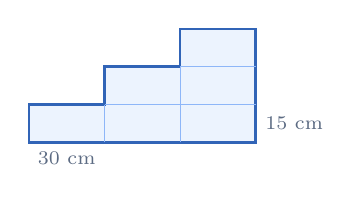
\begin{tikzpicture}[scale=0.032]
\draw[geo,fill=tmBlue!10] (0,0)--(90,0)--(90,45)--(60,45)--(60,30)--(30,30)--(30,15)--(0,15)--cycle;
\draw[tmBlue!60,line width=0.35pt] (30,0)--(30,15) (60,0)--(60,30) (30,15)--(90,15) (60,30)--(90,30);
\node[dim,below] at (15,0){$30$ cm}; \node[dim,right] at (90,7.5){$15$ cm};
\end{tikzpicture}
\end{minipage}
\end{probbox}
\probsol{
Chia khối bậc thang thành ba lớp, mỗi lớp cao $15$ cm $=0{,}15$ m:\par
lớp dưới sâu $0{,}9$ m, lớp giữa sâu $0{,}6$ m, lớp trên sâu $0{,}3$ m.\par
Thể tích: $1{,}5\times0{,}15\times(0{,}9+0{,}6+0{,}3)=1{,}5\times0{,}15\times1{,}8=0{,}405$ m$^3$.
\dapso{$0{,}405$ m$^3$.}}
\gap
\begin{probbox}{50}{\stars{2}}
Một bể nước dài $1{,}5$ m, mực nước trong bể cao $60$ cm. Đổ thêm $240$ l nước thì mực nước cao $80$ cm. Tính chiều rộng của bể.
\end{probbox}
\probsol{
$240$ l $=240$ dm$^3$; nước dâng thêm $80-60=20$ cm $=2$ dm.\par
Diện tích đáy: $240:2=120$ dm$^2=1{,}2$ m$^2$.\par
Chiều rộng: $1{,}2:1{,}5=0{,}8$ m.
\dapso{$0{,}8$ m.}}
\clearpage
\titlehead
\begingroup\setbox0=\vbox{\section*{Xếp hình, sơn bề mặt}}\endgroup
\chapterhead{5}{Xếp hình, sơn bề mặt}
\tikzset{xhf/.style={draw=tmBlue!70!black,line width=0.45pt,line join=round}}
\providecommand{\xhcuboid}{}\renewcommand{\xhcuboid}[7][tmBlue]{\begin{scope}[shift={({#2+0.5*(#3)},{#4+0.35*(#3)})}]
\filldraw[xhf,fill=#1!22] (0,0) rectangle (#5,#7);
\filldraw[xhf,fill=#1!8] (0,#7)--(#5,#7)--({#5+0.5*(#6)},{#7+0.35*(#6)})--({0.5*(#6)},{#7+0.35*(#6)})--cycle;
\filldraw[xhf,fill=#1!45] (#5,0)--({#5+0.5*(#6)},{0.35*(#6)})--({#5+0.5*(#6)},{#7+0.35*(#6)})--(#5,#7)--cycle;
\end{scope}}
\providecommand{\xhcube}{}\renewcommand{\xhcube}[4][tmBlue]{\xhcuboid[#1]{#2}{#3}{#4}{1}{1}{1}}

\shead{Xếp các khối nhỏ thành hình hộp}
\begin{knowbox}
\begin{minipage}[t]{0.62\linewidth}
Khi xếp khít các khối nhỏ bằng nhau (hình lập phương đơn vị, hình lập phương nhỏ, viên gạch) thành một khối mới thì \textbf{thể tích của khối mới} bằng tổng thể tích các khối nhỏ:
\[V_{\text{khối lớn}}=V_{\text{một khối nhỏ}}\times\text{số khối nhỏ}.\]
Để tính diện tích xung quanh, diện tích toàn phần, thể tích của khối hộp xếp từ các khối nhỏ bằng nhau:\par
\smallskip
\textbf{Bước 1.} Tìm các kích thước của khối hộp lớn:\par
chiều dài lớn $=$ chiều dài khối nhỏ $\times$ số khối xếp theo chiều dài;\par
chiều rộng lớn $=$ chiều rộng khối nhỏ $\times$ số khối xếp theo chiều rộng;\par
chiều cao lớn $=$ chiều cao khối nhỏ $\times$ số lớp.\par
\smallskip
\textbf{Bước 2.} Áp dụng công thức của hình hộp chữ nhật, hình lập phương.
\end{minipage}\hfill
\begin{minipage}[t]{0.34\linewidth}\vspace{4pt}\centering
\begin{tikzpicture}[scale=0.62]
\xhcube{0}{1}{0}\xhcube{1}{1}{0}\xhcube{2}{1}{0}\xhcube{0}{1}{1}\xhcube{1}{1}{1}\xhcube{2}{1}{1}\xhcube{0}{0}{0}\xhcube{1}{0}{0}\xhcube{2}{0}{0}\xhcube{0}{0}{1}\xhcube{1}{0}{1}\xhcube{2}{0}{1}
\node[dim,below] at (1.5,0){$3$ hình};
\node[dim,right] at (4,0.6){$2$ lớp};
\end{tikzpicture}\par\smallskip
{\small $3\times2\times2=12$ hình}
\end{minipage}
\end{knowbox}

\shead{Xếp được bao nhiêu hình lập phương vào hộp?}
\begin{knowbox}
Để xếp các hình lập phương cạnh $a$ vào một cái hộp (các độ dài cùng một đơn vị đo):\par
\smallskip
-- theo mỗi cạnh của hộp, tìm xem xếp được bao nhiêu lần độ dài $a$ (lấy thương; phần dư để trống);\par
-- số hình lập phương $=$ (số hình theo chiều dài) $\times$ (số hình theo chiều rộng) $\times$ (số hình theo chiều cao).\par
\smallskip
Nếu xếp các hình lập phương nhỏ thành một hình lập phương lớn thì cạnh hình lớn gấp cạnh hình nhỏ một số tự nhiên lần, do đó
\[\text{số hình lập phương nhỏ}=n\times n\times n,\qquad n=\text{cạnh lớn}:\text{cạnh nhỏ}.\]
Nếu biết diện tích toàn phần của hình lập phương lớn thì diện tích một mặt là $S_{tp}:6$; cạnh là số nhân với chính nó bằng diện tích một mặt.
\end{knowbox}

\shead{Sơn bề mặt khối hình tạo bởi các hình lập phương nhỏ}
\begin{knowbox}
\begin{minipage}[t]{0.6\linewidth}
Hình lập phương lớn có $n$ hình lập phương nhỏ trên mỗi cạnh ($n\ge3$) được sơn cả $6$ mặt rồi tách rời ra:\par
\smallskip
-- \textbf{được sơn $3$ mặt}: các hình ở $8$ đỉnh: $8$ hình;\par
-- \textbf{được sơn đúng $2$ mặt}: nằm trên $12$ cạnh, trừ các hình ở đỉnh: $12\times(n-2)$;\par
-- \textbf{được sơn đúng $1$ mặt}: nằm trên $6$ mặt, không nằm trên cạnh: $6\times(n-2)\times(n-2)$;\par
-- \textbf{không được sơn mặt nào}: phần lõi bên trong, là hình lập phương có $n-2$ hình trên mỗi cạnh: $(n-2)\times(n-2)\times(n-2)$.\par
\smallskip
Với hình hộp chữ nhật có $a;\ b;\ c$ hình nhỏ trên các cạnh (đều $\ge3$): sơn $3$ mặt: $8$; đúng $2$ mặt: $4\times[(a-2)+(b-2)+(c-2)]$; đúng $1$ mặt: $2\times[(a-2)(b-2)+(b-2)(c-2)+(a-2)(c-2)]$; không sơn: $(a-2)(b-2)(c-2)$.
\end{minipage}\hfill
\begin{minipage}[t]{0.37\linewidth}\vspace{4pt}\centering
\begin{tikzpicture}[scale=0.5]
\xhcube[tmOrange]{0}{3}{0}\xhcube[tmGreen]{1}{3}{0}\xhcube[tmGreen]{2}{3}{0}\xhcube[tmOrange]{3}{3}{0}\xhcube[tmGreen]{0}{3}{1}\xhcube[tmBlue]{1}{3}{1}\xhcube[tmBlue]{2}{3}{1}\xhcube[tmGreen]{3}{3}{1}\xhcube[tmGreen]{0}{3}{2}\xhcube[tmBlue]{1}{3}{2}\xhcube[tmBlue]{2}{3}{2}\xhcube[tmGreen]{3}{3}{2}\xhcube[tmOrange]{0}{3}{3}\xhcube[tmGreen]{1}{3}{3}\xhcube[tmGreen]{2}{3}{3}\xhcube[tmOrange]{3}{3}{3}\xhcube[tmGreen]{0}{2}{0}\xhcube[tmBlue]{1}{2}{0}\xhcube[tmBlue]{2}{2}{0}\xhcube[tmGreen]{3}{2}{0}\xhcube[tmBlue]{0}{2}{1}\xhcube[tmBlue]{3}{2}{1}\xhcube[tmBlue]{0}{2}{2}\xhcube[tmBlue]{3}{2}{2}\xhcube[tmGreen]{0}{2}{3}\xhcube[tmBlue]{1}{2}{3}\xhcube[tmBlue]{2}{2}{3}\xhcube[tmGreen]{3}{2}{3}\xhcube[tmGreen]{0}{1}{0}\xhcube[tmBlue]{1}{1}{0}\xhcube[tmBlue]{2}{1}{0}\xhcube[tmGreen]{3}{1}{0}\xhcube[tmBlue]{0}{1}{1}\xhcube[tmBlue]{3}{1}{1}\xhcube[tmBlue]{0}{1}{2}\xhcube[tmBlue]{3}{1}{2}\xhcube[tmGreen]{0}{1}{3}\xhcube[tmBlue]{1}{1}{3}\xhcube[tmBlue]{2}{1}{3}\xhcube[tmGreen]{3}{1}{3}\xhcube[tmOrange]{0}{0}{0}\xhcube[tmGreen]{1}{0}{0}\xhcube[tmGreen]{2}{0}{0}\xhcube[tmOrange]{3}{0}{0}\xhcube[tmGreen]{0}{0}{1}\xhcube[tmBlue]{1}{0}{1}\xhcube[tmBlue]{2}{0}{1}\xhcube[tmGreen]{3}{0}{1}\xhcube[tmGreen]{0}{0}{2}\xhcube[tmBlue]{1}{0}{2}\xhcube[tmBlue]{2}{0}{2}\xhcube[tmGreen]{3}{0}{2}\xhcube[tmOrange]{0}{0}{3}\xhcube[tmGreen]{1}{0}{3}\xhcube[tmGreen]{2}{0}{3}\xhcube[tmOrange]{3}{0}{3}
\end{tikzpicture}\par\smallskip
{\scriptsize\textcolor{tmOrange}{\rule{6pt}{6pt}}\,$3$ mặt\quad\textcolor{tmGreen}{\rule{6pt}{6pt}}\,$2$ mặt\quad\textcolor{tmBlue}{\rule{6pt}{6pt}}\,$1$ mặt}
\end{minipage}\par
\smallskip
\emph{Kiểm tra:} tổng bốn nhóm bằng số hình lập phương nhỏ. Nếu có cạnh chỉ gồm ít hơn $3$ hình nhỏ thì ta đếm trực tiếp.
\end{knowbox}

\shead{Đếm hình lập phương trong khối xếp. Hình nhìn từ các phía}
\begin{knowbox}
\begin{minipage}[t]{0.6\linewidth}
Để đếm số hình lập phương trong một khối xếp, ta đếm \textbf{theo từng cột} (hoặc theo từng lớp). Nếu đề bài không nói gì khác thì mỗi hình đều đặt trên mặt bàn hoặc trên một hình khác, nên các hình bị che khuất nằm bên dưới các hình nhìn thấy.\par
\smallskip
\textbf{Hình nhìn từ trên xuống có ghi số} cho biết các ô ở đáy; số ghi trong mỗi ô là số hình lập phương xếp chồng ở ô đó. Số hình lập phương bằng tổng các số ghi trong ô.\par
\smallskip
Ở \textbf{hình nhìn từ phía trước}, mỗi cột cao bằng chồng cao nhất của cột đó.
\end{minipage}\hfill
\begin{minipage}[t]{0.36\linewidth}\vspace{2pt}\centering
\begin{tikzpicture}[scale=0.5]
\foreach \x/\y/\h in {0/1/2,1/1/3,2/1/1,0/0/1,1/0/2,2/0/1}{\draw[xhf,fill=tmBlue!8] (\x,\y) rectangle ++(1,1); \node[font=\small\bfseries] at (\x+0.5,\y+0.5){\h};}
\node[dim,below] at (1.5,0){phía trước};
\node[dim,above] at (1.5,2){nhìn từ trên xuống};
\end{tikzpicture}\par\smallskip
$2+3+1+1+2+1=10$ hình
\end{minipage}
\end{knowbox}
\gap
\begin{exbox}{\ExWord\ 1}
\begin{minipage}[t]{0.6\linewidth}
Một viên gạch dạng hình hộp chữ nhật có chiều dài $24$ cm, chiều rộng $12$ cm, chiều cao $6$ cm. Bác thợ xây xếp $6$ viên gạch như thế thành một khối gạch dạng hình hộp chữ nhật: mỗi lớp $2$ viên đặt cạnh nhau, xếp $3$ lớp (như hình bên).\par
\pa{a} Tính diện tích xung quanh và diện tích toàn phần của khối gạch đó.\par
\pa{b} Tính thể tích của khối gạch đó.
\end{minipage}\hfill
\begin{minipage}[t]{0.36\linewidth}\vspace{0pt}\centering
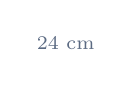
\begin{tikzpicture}[scale=0.085]
\xhcuboid[tmOrange]{0}{12}{0}{24}{12}{6}\xhcuboid[tmOrange]{0}{12}{6}{24}{12}{6}\xhcuboid[tmOrange]{0}{12}{12}{24}{12}{6}
\xhcuboid[tmOrange]{0}{0}{0}{24}{12}{6}\xhcuboid[tmOrange]{0}{0}{6}{24}{12}{6}\xhcuboid[tmOrange]{0}{0}{12}{24}{12}{6}
\node[dim,below] at (12,0){$24$ cm};
\end{tikzpicture}
\end{minipage}
\guide
\pa{a} Chiều dài khối gạch là $24$ cm.\par
Chiều rộng khối gạch là: $12\times2=24$ (cm).\par
Chiều cao khối gạch là: $6\times3=18$ (cm).\par
Diện tích xung quanh của khối gạch là: $(24+24)\times2\times18=1\,728$ (cm$^2$).\par
Diện tích mặt đáy của khối gạch là: $24\times24=576$ (cm$^2$).\par
Diện tích toàn phần của khối gạch là: $1\,728+576\times2=2\,880$ (cm$^2$).\par
\pa{b} \emph{Cách 1.} Thể tích khối gạch là: $24\times24\times18=10\,368$ (cm$^3$).\par
\emph{Cách 2.} Thể tích một viên gạch là: $24\times12\times6=1\,728$ (cm$^3$).\par
Thể tích khối gạch là: $1\,728\times6=10\,368$ (cm$^3$).
\dapso{\pa{a} $1\,728$ cm$^2$; $2\,880$ cm$^2$;\par \pa{b} $10\,368$ cm$^3$.}
\end{exbox}
\gap
\begin{exbox}{\ExWord\ 2}
Người ta xếp các hình lập phương nhỏ cạnh $2$ cm thành một hình lập phương lớn có diện tích toàn phần là $864$ cm$^2$. Hỏi đã dùng bao nhiêu hình lập phương nhỏ?
\guide
\emph{Cách 1.} Diện tích một mặt của hình lập phương lớn là: $864:6=144$ (cm$^2$).\par
Ta có $144=12\times12$ nên cạnh hình lập phương lớn dài $12$ cm.\par
Mỗi cạnh của hình lập phương lớn có: $12:2=6$ (hình nhỏ).\par
Số hình lập phương nhỏ là: $6\times6\times6=216$ (hình).\par
\emph{Cách 2.} Cạnh hình lập phương lớn dài $12$ cm (như trên).\par
Thể tích hình lập phương lớn là: $12\times12\times12=1\,728$ (cm$^3$).\par
Thể tích một hình lập phương nhỏ là: $2\times2\times2=8$ (cm$^3$).\par
Số hình lập phương nhỏ là: $1\,728:8=216$ (hình).
\dapso{$216$ hình.}
\end{exbox}
\gap
\begin{exbox}{\ExWord\ 3}
Một cái thùng dạng hình hộp chữ nhật dài $1{,}2$ m, rộng $0{,}8$ m, cao $0{,}5$ m.\par
\pa{a} Nếu xếp các khối gỗ đồ chơi hình lập phương cạnh $1$ dm vào thùng thì xếp được nhiều nhất bao nhiêu khối?\par
\pa{b} Nếu xếp các hộp quà hình lập phương cạnh $3$ dm vào thùng thì xếp được nhiều nhất bao nhiêu hộp?
\guide
Đổi: $1{,}2$ m $=12$ dm; $0{,}8$ m $=8$ dm; $0{,}5$ m $=5$ dm.\par
\pa{a} Theo chiều dài xếp được $12:1=12$ (khối); theo chiều rộng $8$ khối; theo chiều cao $5$ khối.\par
Số khối gỗ xếp được là: $12\times8\times5=480$ (khối).\par
\pa{b} Theo chiều dài xếp được: $12:3=4$ (hộp).\par
Vì $8:3=2$ (dư $2$ dm) nên theo chiều rộng xếp được $2$ hộp.\par
Vì $5:3=1$ (dư $2$ dm) nên theo chiều cao xếp được $1$ hộp.\par
Số hộp quà xếp được là: $4\times2\times1=8$ (hộp).
\dapso{\pa{a} $480$ khối;\par \pa{b} $8$ hộp.}
\end{exbox}
\gap
\begin{exbox}{\ExWord\ 4}
Mai dán các hình lập phương nhỏ cạnh $1$ cm thành một hình lập phương lớn cạnh $5$ cm rồi sơn cả $6$ mặt ngoài.\par
\pa{a} Mai đã dùng bao nhiêu hình lập phương nhỏ?\par
\pa{b} Có bao nhiêu hình lập phương nhỏ được sơn $3$ mặt? Sơn đúng $2$ mặt? Sơn đúng $1$ mặt? Không được sơn mặt nào?
\guide
\pa{a} Mỗi cạnh có: $5:1=5$ (hình nhỏ).\par Số hình lập phương nhỏ là: $5\times5\times5=125$ (hình).\par
\pa{b} Các hình được sơn $3$ mặt nằm ở $8$ đỉnh: có $8$ hình.\par
Mỗi cạnh có $5-2=3$ hình không nằm ở đỉnh.\par
Số hình được sơn đúng $2$ mặt là: $12\times3=36$ (hình).\par
Mỗi mặt có $3\times3=9$ hình không nằm trên cạnh.\par
Số hình được sơn đúng $1$ mặt là: $6\times9=54$ (hình).\par
Các hình không được sơn tạo thành hình lập phương lõi có $3$ hình trên mỗi cạnh: $3\times3\times3=27$ (hình).\par
\emph{Thử lại:} $8+36+54+27=125$.
\dapso{\pa{a} $125$ hình;\par \pa{b} $8$ hình; $36$ hình; $54$ hình; $27$ hình.}
\end{exbox}
\gap
\begin{exbox}{\ExWord\ 5}
\begin{minipage}[t]{0.58\linewidth}
Nam xếp các hình lập phương thành khối như hình bên.\par
\pa{a} Khối đó có bao nhiêu hình lập phương?\par
\pa{b} Vẽ hình nhìn từ phía trước.\par
\pa{c} Nam cần thêm ít nhất bao nhiêu hình lập phương để được một khối hộp chữ nhật dài $3$ hình, rộng $2$ hình, cao $3$ hình?
\end{minipage}\hfill
\begin{minipage}[t]{0.38\linewidth}\vspace{0pt}\centering
\begin{tikzpicture}[scale=0.5]
\xhcube{0}{1}{0}\xhcube{1}{1}{0}\xhcube{2}{1}{0}\xhcube{0}{1}{1}\xhcube{1}{1}{1}\xhcube{1}{1}{2}\xhcube{0}{0}{0}\xhcube{1}{0}{0}\xhcube{2}{0}{0}\xhcube{1}{0}{1}
\node[dim,below] at (1.5,0){phía trước};
\end{tikzpicture}
\end{minipage}
\guide
\pa{a} Ghi số hình lập phương ở mỗi ô đáy (hình nhìn từ trên xuống):\par
\begin{center}\begin{tikzpicture}[scale=0.45]
\foreach \x/\y/\h in {0/1/2,1/1/3,2/1/1,0/0/1,1/0/2,2/0/1}{\draw[xhf,fill=tmBlue!8] (\x,\y) rectangle ++(1,1); \node[font=\small\bfseries] at (\x+0.5,\y+0.5){\h};}
\node[dim,below] at (1.5,0){phía trước};
\end{tikzpicture}\qquad
\begin{tikzpicture}[scale=0.45]
\foreach \x/\y in {0/0,0/1,1/0,1/1,1/2,2/0}{\draw[xhf,fill=tmBlue!20] (\x,\y) rectangle ++(1,1);}
\node[dim,below] at (1.5,0){nhìn từ phía trước};
\end{tikzpicture}\end{center}
Hàng sau có: $2+3+1=6$ (hình); hàng trước có: $1+2+1=4$ (hình).\par
Khối đó có: $6+4=10$ (hình).\par
\pa{b} Các cột của hình nhìn từ phía trước cao bằng chồng cao nhất: $2$; $3$; $1$ (hình trên).\par
\pa{c} Khối hộp chữ nhật có: $3\times2\times3=18$ (hình).\par
Cần thêm: $18-10=8$ (hình).
\dapso{\pa{a} $10$ hình;\par \pa{c} $8$ hình.}
\end{exbox}
\dividerbar{Luyện tập}
\begin{probbox}{1}{\relax}
Cần bao nhiêu hình lập phương cạnh $1$ cm để xếp thành một hình lập phương cạnh $6$ cm?
\end{probbox}
\probsol{
Mỗi cạnh có: $6:1=6$ (hình nhỏ).\par
Số hình lập phương nhỏ cần dùng là: $6\times6\times6=216$ (hình).
\dapso{$216$ hình.}}
\gap
\begin{probbox}{2}{\relax}
Cần bao nhiêu hình lập phương cạnh $3$ cm để xếp thành một hình lập phương cạnh $12$ cm?
\end{probbox}
\probsol{
Mỗi cạnh có: $12:3=4$ (hình nhỏ).\par
Số hình lập phương nhỏ cần dùng là: $4\times4\times4=64$ (hình).
\dapso{$64$ hình.}}
\gap
\begin{probbox}{3}{\relax}
Cần bao nhiêu hình lập phương cạnh $2$ cm để xếp đầy một cái hộp dài $10$ cm, rộng $8$ cm, cao $6$ cm?
\end{probbox}
\probsol{
Theo chiều dài: $10:2=5$ (hình); theo chiều rộng: $8:2=4$ (hình); theo chiều cao: $6:2=3$ (hình).\par
Số hình lập phương cần dùng là: $5\times4\times3=60$ (hình).
\dapso{$60$ hình.}}
\gap
\begin{probbox}{4}{\relax}
Một cái hòm đựng đồ chơi dài $1{,}2$ m, rộng $0{,}6$ m, cao $0{,}4$ m. Cần bao nhiêu khối gỗ hình lập phương cạnh $2$ dm để xếp đầy khít hòm?
\end{probbox}
\probsol{
Đổi: $1{,}2$ m $=12$ dm; $0{,}6$ m $=6$ dm; $0{,}4$ m $=4$ dm.\par
Theo chiều dài: $12:2=6$ (khối); theo chiều rộng: $6:2=3$ (khối); theo chiều cao: $4:2=2$ (khối).\par
Số khối gỗ cần dùng là: $6\times3\times2=36$ (khối).
\dapso{$36$ khối.}}
\gap
\begin{probbox}{5}{\relax}
Xếp $64$ hình lập phương nhỏ, mỗi hình có thể tích $1$ cm$^3$, thành một hình lập phương lớn. Tính diện tích xung quanh, diện tích toàn phần và thể tích của hình lập phương lớn.
\end{probbox}
\probsol{
Hình lập phương nhỏ có thể tích $1$ cm$^3$ thì có cạnh $1$ cm.\par
Ta có $64=4\times4\times4$ nên mỗi cạnh hình lớn có $4$ hình nhỏ; cạnh hình lớn dài $4$ cm.\par
Diện tích xung quanh là: $4\times4\times4=64$ (cm$^2$).\par
Diện tích toàn phần là: $4\times4\times6=96$ (cm$^2$).\par
Thể tích là: $64\times1=64$ (cm$^3$).
\dapso{$64$ cm$^2$; $96$ cm$^2$; $64$ cm$^3$.}}
\gap
\begin{probbox}{6}{\relax}
Xếp $125$ hình lập phương nhỏ, mỗi hình có thể tích $27$ cm$^3$, thành một hình lập phương lớn. Tính diện tích toàn phần và thể tích của hình lập phương lớn.
\end{probbox}
\probsol{
Ta có $27=3\times3\times3$ nên cạnh hình lập phương nhỏ dài $3$ cm.\par
Ta có $125=5\times5\times5$ nên mỗi cạnh hình lớn có $5$ hình nhỏ.\par
Cạnh hình lập phương lớn là: $3\times5=15$ (cm).\par
Diện tích toàn phần là: $15\times15\times6=1\,350$ (cm$^2$).\par
Thể tích là: $27\times125=3\,375$ (cm$^3$).
\dapso{$1\,350$ cm$^2$; $3\,375$ cm$^3$.}}
\gap
\begin{probbox}{7}{\relax}
Người ta xếp các hình lập phương nhỏ cạnh $1$ cm thành một hình lập phương lớn có diện tích toàn phần $216$ cm$^2$. Hỏi đã dùng bao nhiêu hình lập phương nhỏ?
\end{probbox}
\probsol{
Diện tích một mặt là: $216:6=36$ (cm$^2$).\par
Ta có $36=6\times6$ nên cạnh hình lập phương lớn dài $6$ cm.\par
Số hình lập phương nhỏ là: $6\times6\times6=216$ (hình).
\dapso{$216$ hình.}}
\gap
\begin{probbox}{8}{\relax}
Người ta xếp các hình lập phương nhỏ cạnh $2$ cm thành một hình lập phương lớn có diện tích xung quanh $400$ cm$^2$. Hỏi đã dùng bao nhiêu hình lập phương nhỏ?
\end{probbox}
\probsol{
Diện tích một mặt là: $400:4=100$ (cm$^2$).\par
Ta có $100=10\times10$ nên cạnh hình lập phương lớn dài $10$ cm.\par
Mỗi cạnh có: $10:2=5$ (hình nhỏ).\par
Số hình lập phương nhỏ là: $5\times5\times5=125$ (hình).
\dapso{$125$ hình.}}
\gap
\begin{probbox}{9}{\relax}
Người ta đặt nằm chồng khít $5$ viên gạch lên nhau, mỗi viên dài $20$ cm, rộng $10$ cm, cao $5$ cm. Tính diện tích xung quanh, diện tích toàn phần và thể tích của chồng gạch.
\end{probbox}
\probsol{
Chồng gạch là hình hộp chữ nhật dài $20$ cm, rộng $10$ cm, cao: $5\times5=25$ (cm).\par
Diện tích xung quanh là: $(20+10)\times2\times25=1\,500$ (cm$^2$).\par
Diện tích toàn phần là: $1\,500+20\times10\times2=1\,900$ (cm$^2$).\par
Thể tích là: $20\times10\times25=5\,000$ (cm$^3$).
\dapso{$1\,500$ cm$^2$; $1\,900$ cm$^2$; $5\,000$ cm$^3$.}}
\gap
\begin{probbox}{10}{\relax}
Xếp chồng hai hình lập phương bằng nhau được một hình hộp chữ nhật cao $16$ cm. Tính diện tích xung quanh và diện tích toàn phần của hình hộp chữ nhật đó.
\end{probbox}
\probsol{
Cạnh mỗi hình lập phương là: $16:2=8$ (cm).\par
Hình hộp chữ nhật dài $8$ cm, rộng $8$ cm, cao $16$ cm.\par
Diện tích xung quanh là: $(8+8)\times2\times16=512$ (cm$^2$).\par
Diện tích toàn phần là: $512+8\times8\times2=640$ (cm$^2$).
\dapso{$512$ cm$^2$; $640$ cm$^2$.}}
\gap
\begin{probbox}{11}{\relax}
Xếp thẳng hàng ba hình lập phương bằng nhau được một hình hộp chữ nhật dài $21$ cm. Tính diện tích toàn phần của hình hộp chữ nhật đó.
\end{probbox}
\probsol{
Cạnh mỗi hình lập phương là: $21:3=7$ (cm). Diện tích một mặt là: $7\times7=49$ (cm$^2$).\par
Bốn mặt dài của hình hộp gồm $3\times4=12$ mặt hình lập phương; hai mặt hai đầu là $2$ mặt nữa.\par
Diện tích toàn phần là: $49\times14=686$ (cm$^2$).\par
\emph{Thử lại:} $2\times(21\times7+21\times7+7\times7)=686$ (cm$^2$).
\dapso{$686$ cm$^2$.}}
\gap
\begin{probbox}{12}{\relax}
Một thùng các-tông dài $60$ cm, rộng $40$ cm, cao $30$ cm. Cần bao nhiêu hộp hình lập phương cạnh $10$ cm để xếp đầy khít thùng?
\end{probbox}
\probsol{
Theo chiều dài: $60:10=6$ (hộp); theo chiều rộng: $40:10=4$ (hộp); theo chiều cao: $30:10=3$ (hộp).\par
Số hộp cần dùng là: $6\times4\times3=72$ (hộp).
\dapso{$72$ hộp.}}
\gap
\begin{probbox}{13}{\relax}
Một ngăn kéo dài $50$ cm, rộng $35$ cm, cao $22$ cm. Có thể xếp vào đó nhiều nhất bao nhiêu hộp hình lập phương cạnh $10$ cm?
\end{probbox}
\probsol{
Theo chiều dài: $50:10=5$ (hộp).\par
Vì $35:10=3$ (dư $5$ cm) nên theo chiều rộng xếp được $3$ hộp.\par
Vì $22:10=2$ (dư $2$ cm) nên theo chiều cao xếp được $2$ hộp.\par
Số hộp xếp được nhiều nhất là: $5\times3\times2=30$ (hộp).
\dapso{$30$ hộp.}}
\gap
\begin{probbox}{14}{\relax}
Một cái thùng dài $9$ dm, rộng $6$ dm, cao $4$ dm. Người ta xếp vào thùng các hộp hình lập phương cạnh $3$ dm.\par
\pa{a} Xếp được nhiều nhất bao nhiêu hộp?\par
\pa{b} Khi đã xếp số hộp đó, phần thùng còn trống có thể tích bao nhiêu?
\end{probbox}
\probsol{
\pa{a} Theo chiều dài: $9:3=3$ (hộp); theo chiều rộng: $6:3=2$ (hộp); theo chiều cao: $4:3=1$ (dư $1$ dm) nên được $1$ hộp.\par
Số hộp xếp được là: $3\times2\times1=6$ (hộp).\par
\pa{b} Thể tích cái thùng là: $9\times6\times4=216$ (dm$^3$).\par
Thể tích $6$ hộp là: $3\times3\times3\times6=162$ (dm$^3$).\par
Phần còn trống là: $216-162=54$ (dm$^3$).
\dapso{\pa{a} $6$ hộp;\par \pa{b} $54$ dm$^3$.}}
\gap
\begin{probbox}{15}{\relax}
Một hình lập phương cạnh $3$ cm được xếp từ các hình lập phương nhỏ cạnh $1$ cm rồi sơn tất cả các mặt. Có bao nhiêu hình nhỏ được sơn $3$ mặt, sơn đúng $2$ mặt, sơn đúng $1$ mặt, không được sơn mặt nào?
\end{probbox}
\probsol{
Mỗi cạnh có $3$ hình nhỏ, trong đó $3-2=1$ hình không nằm ở đỉnh.\par
Sơn $3$ mặt: $8$ hình.\par
Sơn đúng $2$ mặt: $12\times1=12$ (hình).\par
Sơn đúng $1$ mặt: $6\times1\times1=6$ (hình).\par
Không được sơn: $1\times1\times1=1$ (hình) -- đó là hình nằm chính giữa.\par
\emph{Thử lại:} $8+12+6+1=27=3\times3\times3$.
\dapso{$8$ hình; $12$ hình; $6$ hình; $1$ hình.}}
\gap
\begin{probbox}{16}{\relax}
Một hình lập phương lớn được xếp từ $216$ hình lập phương nhỏ bằng nhau rồi sơn tất cả các mặt. Hỏi có bao nhiêu hình nhỏ được sơn đúng $2$ mặt? Bao nhiêu hình nhỏ được sơn đúng $1$ mặt?
\end{probbox}
\probsol{
Ta có $216=6\times6\times6$ nên mỗi cạnh có $6$ hình nhỏ.\par
Số hình được sơn đúng $2$ mặt là: $12\times(6-2)=48$ (hình).\par
Số hình được sơn đúng $1$ mặt là: $6\times4\times4=96$ (hình).
\dapso{$48$ hình; $96$ hình.}}
\gap
\begin{probbox}{17}{\relax}
Một hình lập phương lớn được xếp từ $343$ hình lập phương nhỏ bằng nhau rồi sơn tất cả các mặt. Hỏi có bao nhiêu hình nhỏ không được sơn mặt nào?
\end{probbox}
\probsol{
Ta có $343=7\times7\times7$ nên mỗi cạnh có $7$ hình nhỏ.\par
Các hình không được sơn tạo thành hình lập phương lõi có $7-2=5$ hình trên mỗi cạnh.\par
Số hình không được sơn là: $5\times5\times5=125$ (hình).
\dapso{$125$ hình.}}
\gap
\begin{probbox}{18}{\relax}
Người ta xếp các hình lập phương nhỏ cạnh $1$ cm thành hình lập phương lớn cạnh $10$ cm rồi sơn tất cả các mặt. Hỏi có bao nhiêu hình nhỏ được sơn ít nhất $2$ mặt?
\end{probbox}
\probsol{
Mỗi cạnh có $10$ hình nhỏ.\par
Số hình được sơn $3$ mặt: $8$ hình.\par
Số hình được sơn đúng $2$ mặt là: $12\times(10-2)=96$ (hình).\par
Số hình được sơn ít nhất $2$ mặt là: $8+96=104$ (hình).
\dapso{$104$ hình.}}
\gap
\begin{probbox}{19}{\relax}
Người ta xếp các hình lập phương nhỏ cạnh $1$ cm thành hình hộp chữ nhật dài $5$ cm, rộng $4$ cm, cao $3$ cm rồi sơn tất cả các mặt. Có bao nhiêu hình nhỏ được sơn $3$ mặt, sơn đúng $2$ mặt, sơn đúng $1$ mặt, không được sơn mặt nào?
\end{probbox}
\probsol{
Trên các cạnh có $5;\ 4;\ 3$ hình nhỏ; bỏ các hình ở đỉnh còn $3;\ 2;\ 1$ hình.\par
Sơn $3$ mặt: $8$ hình.\par
Sơn đúng $2$ mặt: $4\times(3+2+1)=24$ (hình).\par
Sơn đúng $1$ mặt: $2\times(3\times2+2\times1+3\times1)=22$ (hình).\par
Không được sơn: $3\times2\times1=6$ (hình).\par
\emph{Thử lại:} $8+24+22+6=60=5\times4\times3$.
\dapso{$8$ hình; $24$ hình; $22$ hình; $6$ hình.}}
\gap
\begin{probbox}{20}{\relax}
Người ta xếp các hình lập phương nhỏ cạnh $2$ cm thành hình hộp chữ nhật dài $14$ cm, rộng $10$ cm, cao $6$ cm rồi sơn tất cả các mặt. Có bao nhiêu hình nhỏ được sơn đúng $2$ mặt, sơn đúng $1$ mặt, không được sơn mặt nào?
\end{probbox}
\probsol{
Trên các cạnh có: $14:2=7$; $10:2=5$; $6:2=3$ (hình); bỏ các hình ở đỉnh còn $5;\ 3;\ 1$ hình.\par
Sơn đúng $2$ mặt: $4\times(5+3+1)=36$ (hình).\par
Sơn đúng $1$ mặt: $2\times(5\times3+3\times1+5\times1)=46$ (hình).\par
Không được sơn: $5\times3\times1=15$ (hình).
\dapso{$36$ hình; $46$ hình; $15$ hình.}}
\gap
\begin{probbox}{21}{\relax}
Một hình lập phương lớn xếp từ các hình lập phương nhỏ bằng nhau được sơn tất cả các mặt. Có đúng $64$ hình nhỏ không được sơn. Hỏi có tất cả bao nhiêu hình nhỏ và có bao nhiêu hình nhỏ được sơn đúng $1$ mặt?
\end{probbox}
\probsol{
Phần lõi không được sơn là hình lập phương: $64=4\times4\times4$ nên mỗi cạnh lõi có $4$ hình.\par
Mỗi cạnh hình lập phương lớn có: $4+2=6$ (hình).\par
Số hình nhỏ là: $6\times6\times6=216$ (hình).\par
Số hình được sơn đúng $1$ mặt là: $6\times4\times4=96$ (hình).
\dapso{$216$ hình; $96$ hình.}}
\gap
\begin{probbox}{22}{\relax}
Một hình lập phương lớn xếp từ các hình lập phương nhỏ bằng nhau được sơn tất cả các mặt. Có đúng $150$ hình nhỏ được sơn đúng $1$ mặt. Hỏi có tất cả bao nhiêu hình nhỏ?
\end{probbox}
\probsol{
Mỗi mặt có: $150:6=25$ (hình) được sơn đúng $1$ mặt; $25=5\times5$.\par
Do đó $n-2=5$, mỗi cạnh có $7$ hình nhỏ.\par
Số hình nhỏ là: $7\times7\times7=343$ (hình).
\dapso{$343$ hình.}}
\gap
\begin{probbox}{23}{\relax}
Xếp các hình lập phương nhỏ cạnh $1$ cm thành một hình lập phương lớn rồi sơn tất cả các mặt. Có đúng $84$ hình nhỏ được sơn $2$ mặt. Tính thể tích hình lập phương lớn.
\end{probbox}
\probsol{
Mỗi cạnh có: $84:12=7$ (hình) được sơn đúng $2$ mặt.\par
Mỗi cạnh có: $7+2=9$ (hình nhỏ), nên cạnh hình lập phương lớn dài $9$ cm.\par
Thể tích là: $9\times9\times9=729$ (cm$^3$).
\dapso{$729$ cm$^3$.}}
\gap
\begin{probbox}{24}{\relax}
Xếp các hình lập phương nhỏ cạnh $1$ cm thành hình lập phương lớn cạnh $5$ cm. Sau đó lấy đi một lớp trên cùng. Hỏi còn lại bao nhiêu hình nhỏ và diện tích toàn phần của khối còn lại là bao nhiêu?
\end{probbox}
\probsol{
Một lớp có: $5\times5=25$ (hình), còn lại: $125-25=100$ (hình).\par
Khối còn lại là hình hộp chữ nhật dài $5$ cm, rộng $5$ cm, cao $4$ cm.\par
Diện tích xung quanh là: $(5+5)\times2\times4=80$ (cm$^2$).\par
Diện tích toàn phần là: $80+5\times5\times2=130$ (cm$^2$).
\dapso{$100$ hình; $130$ cm$^2$.}}
\gap
\begin{probbox}{25}{\relax}
Xếp các hình lập phương nhỏ cạnh $1$ cm thành hình lập phương lớn cạnh $4$ cm. Lấy đi một hình nhỏ ở một đỉnh. Tính diện tích toàn phần của khối còn lại.
\end{probbox}
\probsol{
Lúc đầu diện tích toàn phần là: $4\times4\times6=96$ (cm$^2$).\par
Lấy hình ở đỉnh đi thì mất $3$ ô vuông $1$ cm$^2$ ở mặt ngoài nhưng lại lộ ra $3$ ô vuông $1$ cm$^2$ mới ở chỗ lõm.\par
Diện tích không thay đổi: $96-3+3=96$ (cm$^2$).
\dapso{$96$ cm$^2$.}}
\gap
\begin{probbox}{26}{\relax}
\begin{minipage}[t]{0.6\linewidth}
Khối bậc thang bên có bao nhiêu hình lập phương? (Phía sau không bị thiếu hình nào.)
\end{minipage}\hfill
\begin{minipage}[t]{0.36\linewidth}\vspace{0pt}\centering
\begin{tikzpicture}[scale=0.45]
\xhcube{0}{1}{0}\xhcube{1}{1}{0}\xhcube{2}{1}{0}\xhcube{1}{1}{1}\xhcube{2}{1}{1}\xhcube{2}{1}{2}\xhcube{0}{0}{0}\xhcube{1}{0}{0}\xhcube{2}{0}{0}\xhcube{1}{0}{1}\xhcube{2}{0}{1}\xhcube{2}{0}{2}
\end{tikzpicture}
\end{minipage}
\end{probbox}
\probsol{
Khối bậc thang có $2$ hàng (trước và sau).\par
Nhìn từ phía trước, các cột có $1;\ 2;\ 3$ hình: mỗi hàng có $1+2+3=6$ (hình).\par
Số hình lập phương là: $6\times2=12$ (hình).
\dapso{$12$ hình.}}
\gap
\begin{probbox}{27}{\relax}
\begin{minipage}[t]{0.6\linewidth}
Hình bên là hình nhìn từ trên xuống của một khối xếp; số trong mỗi ô cho biết có bao nhiêu hình lập phương xếp chồng ở ô đó.\par
\pa{a} Khối đó có bao nhiêu hình lập phương?\par
\pa{b} Ở hình nhìn từ phía trước, mỗi cột cao bao nhiêu hình?
\end{minipage}\hfill
\begin{minipage}[t]{0.36\linewidth}\vspace{0pt}\centering
\begin{tikzpicture}[scale=0.5]
\foreach \x/\y/\h in {0/1/3,1/1/1,2/1/2,0/0/2,1/0/2,2/0/1}{\draw[xhf,fill=tmBlue!8] (\x,\y) rectangle ++(1,1); \node[font=\small\bfseries] at (\x+0.5,\y+0.5){\h};}
\node[dim,below] at (1.5,0){phía trước};
\end{tikzpicture}
\end{minipage}
\end{probbox}
\probsol{
\pa{a} Số hình lập phương là: $3+1+2+2+2+1=11$ (hình).\par
\pa{b} Từ trái sang phải, chồng cao nhất ở mỗi cột có $3;\ 2;\ 2$ hình.
\dapso{\pa{a} $11$ hình;\par \pa{b} $3;\ 2;\ 2$ hình.}}
\gap
\begin{probbox}{28}{\relax}
\begin{minipage}[t]{0.6\linewidth}
Khối xếp bên có bao nhiêu hình lập phương? Cần thêm bao nhiêu hình nữa thì đủ để xếp một hình lập phương có $3$ hình nhỏ trên mỗi cạnh?
\end{minipage}\hfill
\begin{minipage}[t]{0.36\linewidth}\vspace{0pt}\centering
\begin{tikzpicture}[scale=0.45]
\xhcube{0}{1}{0}\xhcube{1}{1}{0}\xhcube{2}{1}{0}\xhcube{0}{1}{1}\xhcube{1}{1}{1}\xhcube{2}{1}{1}\xhcube{0}{1}{2}\xhcube{1}{1}{2}\xhcube{2}{1}{2}\xhcube{0}{0}{0}\xhcube{1}{0}{0}\xhcube{2}{0}{0}\xhcube{0}{0}{1}\xhcube{1}{0}{1}\xhcube{2}{0}{1}
\end{tikzpicture}
\end{minipage}
\end{probbox}
\probsol{
Hàng trước có: $3\times2=6$ (hình); hàng sau có: $3\times3=9$ (hình).\par
Khối xếp có: $6+9=15$ (hình).\par
Hình lập phương có $3$ hình nhỏ trên mỗi cạnh gồm: $3\times3\times3=27$ (hình).\par
Cần thêm: $27-15=12$ (hình).
\dapso{$15$ hình; thêm $12$ hình.}}
\gap
\begin{probbox}{29}{\relax}
Khoa xếp $64$ con xúc xắc, mỗi con là hình lập phương cạnh $2$ cm, thành một hình lập phương lớn. Tính diện tích toàn phần và thể tích của hình lập phương lớn.
\end{probbox}
\probsol{
Ta có $64=4\times4\times4$ nên mỗi cạnh có $4$ con xúc xắc.\par
Cạnh hình lập phương lớn là: $2\times4=8$ (cm).\par
Diện tích toàn phần là: $8\times8\times6=384$ (cm$^2$).\par
Thể tích là: $8\times8\times8=512$ (cm$^3$).
\dapso{$384$ cm$^2$; $512$ cm$^3$.}}
\gap
\begin{probbox}{30}{\relax}
Người ta sơn tất cả các mặt của một khối gỗ hình hộp chữ nhật dài $12$ dm, rộng $8$ dm, cao $6$ dm, sau đó xẻ thành các khối lập phương cạnh $2$ dm. Hỏi có bao nhiêu khối lập phương? Bao nhiêu khối không được sơn mặt nào? Bao nhiêu khối được sơn đúng $1$ mặt?
\end{probbox}
\probsol{
Trên các cạnh có: $12:2=6$; $8:2=4$; $6:2=3$ (khối).\par
Số khối lập phương là: $6\times4\times3=72$ (khối).\par
Bỏ các khối ở đỉnh, trên các cạnh còn $4;\ 2;\ 1$ khối.\par
Không được sơn: $4\times2\times1=8$ (khối).\par
Sơn đúng $1$ mặt: $2\times(4\times2+2\times1+4\times1)=28$ (khối).
\dapso{$72$ khối; $8$ khối; $28$ khối.}}
\dividerbar{Thử thách -- Nâng cao}
\begin{probbox}{31}{\stars{1}}
Một hình lập phương lớn xếp từ các hình lập phương nhỏ được sơn tất cả các mặt. Số hình nhỏ được sơn đúng $1$ mặt bằng số hình nhỏ được sơn đúng $2$ mặt. Hỏi hình lập phương lớn gồm bao nhiêu hình nhỏ?
\end{probbox}
\probsol{
Gọi số hình nhỏ trên mỗi cạnh là $n$, đặt $k=n-2$.\par
Sơn đúng $1$ mặt: $6\times k\times k$; sơn đúng $2$ mặt: $12\times k$.\par
$6\times k\times k=12\times k$ nên $k=2$, do đó $n=4$.\par
Số hình nhỏ là: $4\times4\times4=64$ (hình).
\dapso{$64$ hình.}}
\gap
\begin{probbox}{32}{\stars{2}}
Một hình lập phương lớn xếp từ các hình lập phương nhỏ được sơn tất cả các mặt. Số hình nhỏ không được sơn bằng số hình nhỏ được sơn đúng $1$ mặt. Hỏi có bao nhiêu hình nhỏ?
\end{probbox}
\probsol{
Đặt $k=n-2$. Không được sơn: $k\times k\times k$; sơn đúng $1$ mặt: $6\times k\times k$.\par
$k\times k\times k=6\times k\times k$ nên $k=6$, do đó $n=8$.\par
Số hình nhỏ là: $8\times8\times8=512$ (hình).\par
\emph{Thử lại:} không sơn $6\times6\times6=216$; sơn $1$ mặt $6\times36=216$.
\dapso{$512$ hình.}}
\gap
\begin{probbox}{33}{\stars{1}}
Một hình lập phương cạnh $4$ cm xếp từ các hình lập phương nhỏ cạnh $1$ cm được sơn tất cả các mặt rồi tách rời ra. Hỏi số mặt được sơn bằng mấy phần tổng số mặt của tất cả các hình nhỏ?
\end{probbox}
\probsol{
Số ô vuông được sơn chính là mặt ngoài hình lớn: $4\times4\times6=96$ (ô).\par
Tổng số mặt của các hình nhỏ là: $64\times6=384$ (mặt).\par
Phân số cần tìm: $\dfrac{96}{384}=\dfrac14$.
\dapso{$\dfrac14$.}}
\gap
\begin{probbox}{34}{\stars{1}}
Xếp các hình lập phương nhỏ cạnh $1$ cm thành hình lập phương lớn cạnh $5$ cm. Chỉ sơn $4$ mặt xung quanh (không sơn mặt trên và mặt dưới). Có bao nhiêu hình nhỏ được sơn đúng $2$ mặt, sơn đúng $1$ mặt, không được sơn mặt nào?
\end{probbox}
\probsol{
Mỗi lớp trong $5$ lớp là một hình vuông $5\times5$ được sơn ở viền ngoài.\par
Trong một lớp: $4$ hình ở góc được sơn $2$ mặt; $4\times3=12$ hình được sơn $1$ mặt; $3\times3=9$ hình không được sơn.\par
Sơn đúng $2$ mặt: $4\times5=20$ (hình).\par
Sơn đúng $1$ mặt: $12\times5=60$ (hình).\par
Không được sơn: $9\times5=45$ (hình).\par
\emph{Thử lại:} $20+60+45=125$.
\dapso{$20$ hình; $60$ hình; $45$ hình.}}
\gap
\begin{probbox}{35}{\stars{2}}
Xếp các hình lập phương nhỏ cạnh $1$ cm thành hình lập phương lớn cạnh $6$ cm. Sơn $4$ mặt xung quanh màu xanh; mặt trên và mặt dưới màu đỏ. Hỏi có bao nhiêu hình nhỏ được sơn cả hai màu?
\end{probbox}
\probsol{
Hình nhỏ có màu đỏ nằm ở lớp trên cùng hoặc lớp dưới cùng.\par
Hình đó có thêm màu xanh khi nằm ở viền ngoài của lớp.\par
Viền ngoài của một lớp $6\times6$ có: $6\times6-4\times4=20$ (hình).\par
Số hình được sơn cả hai màu là: $20\times2=40$ (hình).
\dapso{$40$ hình.}}
\gap
\begin{probbox}{36}{\stars{1}}
Xếp $343$ hình lập phương nhỏ cạnh $2$ cm thành một hình lập phương lớn. Sau đó lấy đi một lớp trên cùng. Tính diện tích toàn phần của khối còn lại.
\end{probbox}
\probsol{
Ta có $343=7\times7\times7$ nên cạnh hình lập phương lớn là: $2\times7=14$ (cm).\par
Lấy đi lớp trên cùng, còn lại hình hộp chữ nhật dài $14$ cm, rộng $14$ cm, cao: $14-2=12$ (cm).\par
Diện tích xung quanh là: $(14+14)\times2\times12=672$ (cm$^2$).\par
Diện tích toàn phần là: $672+14\times14\times2=1\,064$ (cm$^2$).
\dapso{$1\,064$ cm$^2$.}}
\gap
\begin{probbox}{37}{\stars{2}}
Xếp các hình lập phương nhỏ cạnh $1$ cm thành hình lập phương lớn cạnh $5$ cm. Sau đó rút ra một hàng hình nhỏ để tạo một đường hầm thẳng, tiết diện $1$ cm $\times$ $1$ cm, xuyên từ chính giữa mặt trước đến chính giữa mặt sau. Hỏi còn lại bao nhiêu hình nhỏ? Diện tích toàn phần của khối lúc này (kể cả mặt trong đường hầm) là bao nhiêu?
\end{probbox}
\probsol{
Đường hầm lấy đi $5$ hình nhỏ, còn lại: $125-5=120$ (hình).\par
Mặt ngoài lúc đầu là: $5\times5\times6=150$ (cm$^2$); hai lỗ hầm làm mất $2$ cm$^2$.\par
Đường hầm có $4$ mặt trong, mỗi mặt dài $5$ cm, rộng $1$ cm: $4\times5=20$ (cm$^2$).\par
Diện tích toàn phần là: $150-2+20=168$ (cm$^2$).
\dapso{$120$ hình; $168$ cm$^2$.}}
\gap
\begin{probbox}{38}{\stars{1}}
Một cái hộp dài $20$ cm, rộng $12$ cm, cao $8$ cm. Người ta xếp đầy khít hộp bằng các hình lập phương bằng nhau có độ dài cạnh là số tự nhiên (đơn vị xăng-ti-mét). Hỏi ít nhất phải dùng bao nhiêu hình lập phương?
\end{probbox}
\probsol{
Muốn dùng ít hình nhất thì cạnh hình lập phương phải lớn nhất.\par
Cạnh đó phải là số mà $20;\ 12;\ 8$ đều chia hết; số lớn nhất như vậy là $4$.\par
Với cạnh $4$ cm: $20:4=5$; $12:4=3$; $8:4=2$.\par
Số hình lập phương ít nhất là: $5\times3\times2=30$ (hình).
\dapso{$30$ hình.}}
\gap
\begin{probbox}{39}{\stars{1}}
Một cái thùng dài $6$ dm, rộng $4$ dm, cao $2$ dm. Người ta xếp đầy khít thùng bằng các hình lập phương bằng nhau có độ dài cạnh là số tự nhiên (đơn vị đề-xi-mét). Hỏi xếp được nhiều nhất bao nhiêu hình? Ít nhất bao nhiêu hình?
\end{probbox}
\probsol{
Nhiều nhất: cạnh $1$ dm, số hình là: $6\times4\times2=48$ (hình).\par
Ít nhất: cạnh phải là số mà $6;\ 4;\ 2$ đều chia hết; số lớn nhất như vậy là $2$.\par
Với cạnh $2$ dm, số hình là: $3\times2\times1=6$ (hình).
\dapso{Nhiều nhất $48$ hình, ít nhất $6$ hình.}}
\gap
\begin{probbox}{40}{\stars{1}}
Người ta dán các hình lập phương cạnh $1$ cm thành một hàng thẳng, mặt áp mặt. Một hàng $10$ hình có diện tích toàn phần $42$ cm$^2$. Hỏi hàng có diện tích toàn phần $82$ cm$^2$ gồm bao nhiêu hình?
\end{probbox}
\probsol{
Mỗi hình cho $4$ mặt ở phía xung quanh của hàng; $2$ đầu hàng thêm $2$ mặt.\par
Hàng $n$ hình có diện tích $4\times n+2$ (cm$^2$). Thử: $4\times10+2=42$.\par
$4\times n+2=82$ nên $4\times n=80$, $n=20$.
\dapso{$20$ hình.}}
\gap
\begin{probbox}{41}{\stars{1}}
\begin{minipage}[t]{0.6\linewidth}
Một khối bậc thang được dán từ các hình lập phương cạnh $1$ cm (chỉ có một hàng). Tính số hình lập phương và diện tích toàn phần của khối bậc thang (kể cả mặt đáy).
\end{minipage}\hfill
\begin{minipage}[t]{0.36\linewidth}\vspace{0pt}\centering
\begin{tikzpicture}[scale=0.42]
\xhcube{0}{0}{0}\xhcube{1}{0}{0}\xhcube{2}{0}{0}\xhcube{3}{0}{0}\xhcube{1}{0}{1}\xhcube{2}{0}{1}\xhcube{3}{0}{1}\xhcube{2}{0}{2}\xhcube{3}{0}{2}\xhcube{3}{0}{3}
\end{tikzpicture}
\end{minipage}
\end{probbox}
\probsol{
Số hình lập phương là: $1+2+3+4=10$ (hình).\par
Mặt trước và mặt sau: $10+10=20$ (cm$^2$).\par
Mặt đáy: $4$ cm$^2$; nhìn từ trên xuống thấy $4$ cm$^2$ (mỗi cột một ô).\par
Hướng sang trái: $1+1+1+1=4$ (cm$^2$) (đầu bên trái và ba bậc đứng); hướng sang phải: $4$ cm$^2$.\par
Diện tích toàn phần là: $20+4+4+4+4=36$ (cm$^2$).
\dapso{$10$ hình; $36$ cm$^2$.}}
\gap
\begin{probbox}{42}{\stars{1}}
\begin{minipage}[t]{0.6\linewidth}
Hình bên là hình nhìn từ trên xuống của một khối xếp, có ghi số hình lập phương ở mỗi ô. Khối đó có bao nhiêu hình lập phương? Cần thêm bao nhiêu hình để được một hình lập phương có $3$ hình nhỏ trên mỗi cạnh?
\end{minipage}\hfill
\begin{minipage}[t]{0.36\linewidth}\vspace{0pt}\centering
\begin{tikzpicture}[scale=0.5]
\foreach \x/\y/\h in {0/2/3,1/2/2,2/2/1,0/1/2,1/1/2,2/1/1,0/0/1,1/0/1,2/0/1}{\draw[xhf,fill=tmBlue!8] (\x,\y) rectangle ++(1,1); \node[font=\small\bfseries] at (\x+0.5,\y+0.5){\h};}
\node[dim,below] at (1.5,0){phía trước};
\end{tikzpicture}
\end{minipage}
\end{probbox}
\probsol{
Số hình lập phương là: $(3+2+1)+(2+2+1)+(1+1+1)=6+5+3=14$ (hình).\par
Hình lập phương đầy đủ có $27$ hình.\par
Cần thêm: $27-14=13$ (hình).
\dapso{$14$ hình; thêm $13$ hình.}}
\gap
\begin{probbox}{43}{\stars{1}}
Một hình lập phương cạnh $6$ cm xếp từ các hình lập phương nhỏ cạnh $1$ cm được sơn tất cả các mặt rồi tách rời ra. Tính tổng diện tích các mặt được sơn và tổng diện tích các mặt không được sơn của tất cả các hình nhỏ.
\end{probbox}
\probsol{
Phần được sơn chính là mặt ngoài hình lớn: $6\times6\times6=216$ (cm$^2$).\par
Có $216$ hình nhỏ, mỗi hình có $6$ mặt $1$ cm$^2$: $216\times6=1\,296$ (cm$^2$).\par
Phần không được sơn là: $1\,296-216=1\,080$ (cm$^2$).
\dapso{Được sơn $216$ cm$^2$; không được sơn $1\,080$ cm$^2$.}}
\gap
\begin{probbox}{44}{\stars{2}}
Một hình hộp chữ nhật xếp từ các hình lập phương cạnh $1$ cm có đáy dài $6$ cm, rộng $5$ cm. Sơn tất cả các mặt thì có $24$ hình nhỏ không được sơn. Tính chiều cao hình hộp và số hình nhỏ được sơn đúng $1$ mặt.
\end{probbox}
\probsol{
Phần lõi không được sơn có mỗi lớp gồm $(6-2)\times(5-2)=4\times3=12$ (hình).\par
Số lớp của lõi là: $24:12=2$ (lớp), nên chiều cao là: $2+2=4$ (cm).\par
Bỏ các hình ở đỉnh, trên các cạnh còn $4;\ 3;\ 2$ hình.\par
Sơn đúng $1$ mặt: $2\times(4\times3+3\times2+4\times2)=2\times26=52$ (hình).
\dapso{Chiều cao $4$ cm; $52$ hình.}}
\gap
\begin{probbox}{45}{\stars{2}}
Người ta dùng các viên gạch dài $12$ cm, rộng $8$ cm, cao $6$ cm, đặt cùng một chiều, xếp cạnh nhau và chồng thành lớp để được một khối đặc hình lập phương. Cần ít nhất bao nhiêu viên gạch?
\end{probbox}
\probsol{
Cạnh hình lập phương phải chia hết cho chiều dài, chiều rộng và chiều cao viên gạch.\par
Số nhỏ nhất chia hết cho $12;\ 8;\ 6$ là $24$, nên cạnh hình lập phương là $24$ cm.\par
Theo chiều dài: $24:12=2$ (viên); theo chiều rộng: $24:8=3$ (viên); theo chiều cao: $24:6=4$ (lớp).\par
Số viên gạch là: $2\times3\times4=24$ (viên).
\dapso{$24$ viên.}}
\gap
\begin{probbox}{46}{\stars{1}}
Một hình lập phương lớn xếp từ các hình lập phương nhỏ được sơn tất cả các mặt. Có đúng $98$ hình nhỏ được sơn. Hỏi mỗi cạnh hình lớn có bao nhiêu hình nhỏ?
\end{probbox}
\probsol{
Số hình được sơn $=$ số hình tất cả $-$ số hình ở lõi.\par
Thử $n=4$: $64-8=56$. Thử $n=5$: $125-27=98$ (đúng).\par
Vậy mỗi cạnh có $5$ hình nhỏ.
\dapso{$5$ hình.}}
\gap
\begin{probbox}{47}{\stars{2}}
\begin{minipage}[t]{0.6\linewidth}
Từ hình lập phương cạnh $4$ cm xếp bởi các hình lập phương nhỏ cạnh $1$ cm, người ta lấy đi cả $8$ hình ở $8$ đỉnh. Hỏi còn lại bao nhiêu hình nhỏ? Diện tích toàn phần của khối còn lại là bao nhiêu?
\end{minipage}\hfill
\begin{minipage}[t]{0.36\linewidth}\vspace{0pt}\centering
\begin{tikzpicture}[scale=0.4]
\xhcube{1}{3}{0}\xhcube{2}{3}{0}\xhcube{0}{3}{1}\xhcube{1}{3}{1}\xhcube{2}{3}{1}\xhcube{3}{3}{1}\xhcube{0}{3}{2}\xhcube{1}{3}{2}\xhcube{2}{3}{2}\xhcube{3}{3}{2}\xhcube{1}{3}{3}\xhcube{2}{3}{3}\xhcube{0}{2}{0}\xhcube{1}{2}{0}\xhcube{2}{2}{0}\xhcube{3}{2}{0}\xhcube{0}{2}{1}\xhcube{1}{2}{1}\xhcube{2}{2}{1}\xhcube{3}{2}{1}\xhcube{0}{2}{2}\xhcube{1}{2}{2}\xhcube{2}{2}{2}\xhcube{3}{2}{2}\xhcube{0}{2}{3}\xhcube{1}{2}{3}\xhcube{2}{2}{3}\xhcube{3}{2}{3}\xhcube{0}{1}{0}\xhcube{1}{1}{0}\xhcube{2}{1}{0}\xhcube{3}{1}{0}\xhcube{0}{1}{1}\xhcube{1}{1}{1}\xhcube{2}{1}{1}\xhcube{3}{1}{1}\xhcube{0}{1}{2}\xhcube{1}{1}{2}\xhcube{2}{1}{2}\xhcube{3}{1}{2}\xhcube{0}{1}{3}\xhcube{1}{1}{3}\xhcube{2}{1}{3}\xhcube{3}{1}{3}\xhcube{1}{0}{0}\xhcube{2}{0}{0}\xhcube{0}{0}{1}\xhcube{1}{0}{1}\xhcube{2}{0}{1}\xhcube{3}{0}{1}\xhcube{0}{0}{2}\xhcube{1}{0}{2}\xhcube{2}{0}{2}\xhcube{3}{0}{2}\xhcube{1}{0}{3}\xhcube{2}{0}{3}
\end{tikzpicture}
\end{minipage}
\end{probbox}
\probsol{
Số hình còn lại là: $64-8=56$ (hình).\par
Mỗi lần lấy đi một hình ở đỉnh thì mất $3$ ô vuông ở mặt ngoài nhưng lộ ra $3$ ô vuông mới, nên diện tích không đổi.\par
Diện tích toàn phần là: $4\times4\times6=96$ (cm$^2$).
\dapso{$56$ hình; $96$ cm$^2$.}}
\gap
\begin{probbox}{48}{\stars{2}}
Xếp các hình lập phương nhỏ cạnh $1$ cm thành hình hộp chữ nhật dài $8$ cm, rộng $6$ cm, cao $4$ cm đặt trên mặt bàn. Sơn tất cả các mặt trừ mặt đáy. Hỏi có bao nhiêu hình nhỏ được sơn đúng $1$ mặt?
\end{probbox}
\probsol{
\emph{Mặt trên:} các hình không nằm ở viền: $(8-2)\times(6-2)=24$ (hình).\par
\emph{Mặt trước và mặt sau:} các hình không nằm ở cạnh trái, cạnh phải (mỗi hàng $6$ hình) và không ở hàng trên cùng (còn $3$ hàng; hàng dưới cùng không bị sơn ở đáy): mỗi mặt $6\times3=18$ (hình), cả hai mặt $36$ hình.\par
\emph{Mặt trái và mặt phải:} mỗi mặt $(6-2)\times3=12$ (hình), cả hai mặt $24$ hình.\par
Số hình được sơn đúng $1$ mặt là: $24+36+24=84$ (hình).
\dapso{$84$ hình.}}
\gap
\begin{probbox}{49}{\stars{2}}
Một hình lập phương được xếp từ $27$ hình lập phương nhỏ ($3$ hình trên mỗi cạnh). Trong đó có tất cả bao nhiêu hình lập phương (gồm các hình có $1$, $2$ hoặc $3$ hình nhỏ trên mỗi cạnh)?
\end{probbox}
\probsol{
Hình lập phương cạnh $1$: $27$ hình.\par
Hình lập phương cạnh $2$: theo mỗi chiều có $2$ vị trí, nên có $2\times2\times2=8$ (hình).\par
Hình lập phương cạnh $3$: $1$ hình.\par
Tất cả có: $27+8+1=36$ (hình).
\dapso{$36$ hình.}}
\gap
\begin{probbox}{50}{\stars{2}}
\begin{minipage}[t]{0.56\linewidth}
Một khối xếp đặt trên đáy gồm $3\times2$ ô vuông, ô nào cũng có ít nhất một hình lập phương. Hình bên là hình nhìn từ phía trước và hình nhìn từ bên phải của khối. Khối đó có nhiều nhất bao nhiêu hình lập phương? Ít nhất bao nhiêu hình?
\end{minipage}\hfill
\begin{minipage}[t]{0.4\linewidth}\vspace{0pt}\centering
\begin{tikzpicture}[scale=0.55]
\foreach \x/\y in {0/0,0/1,0/2,1/0,2/0,2/1}{\draw[xhf,fill=tmBlue!20] (\x,\y) rectangle ++(1,1);}
\node[dim,below] at (1.5,0){từ phía trước};
\begin{scope}[shift={(5,0)}]
\foreach \x/\y in {0/0,0/1,1/0,1/1,1/2}{\draw[xhf,fill=tmBlue!20] (\x,\y) rectangle ++(1,1);}
\node[dim,below,align=center] at (1,0){từ bên phải\\(trước\,|\,sau)};
\end{scope}
\end{tikzpicture}
\end{minipage}
\end{probbox}
\probsol{
Nhìn từ phía trước: ba cột (từ trái sang phải) cao $3;\ 1;\ 2$ hình. Nhìn từ bên phải: hàng trước cao $2$ hình, hàng sau cao $3$ hình.\par
\emph{Nhiều nhất:} mỗi chồng cao bằng số bé hơn trong hai số: chiều cao của cột và chiều cao của hàng chứa nó.\par
Hàng trước: $2+1+2=5$ (hình); hàng sau: $3+1+2=6$ (hình). Nhiều nhất: $5+6=11$ (hình).\par
\emph{Ít nhất:} đặt $3$ hình ở ô bên trái hàng sau (vừa đủ cột trái cao $3$, vừa đủ hàng sau cao $3$), đặt $2$ hình ở ô bên phải hàng trước; mỗi ô còn lại $1$ hình.\par
Ít nhất: $3+2+1+1+1+1=9$ (hình).
\dapso{Nhiều nhất $11$ hình, ít nhất $9$ hình.}}
\clearpage
\titlehead
\begingroup\setbox0=\vbox{\section*{Chuyển động đều}}\endgroup
\chapterhead{6}{Chuyển động đều}
\shead{Vận tốc, quãng đường, thời gian}
\begin{knowbox}
\begin{minipage}[t]{0.6\linewidth}
\textbf{Bài toán chuyển động} là bài toán về người hoặc vật di chuyển từ vị trí A đến vị trí B trong một khoảng thời gian nhất định.\par
\smallskip
-- Độ dài AB gọi là \textbf{quãng đường}, kí hiệu $s$ (thường tính bằng km).\par
-- Thời gian đi từ A đến B gọi là \textbf{thời gian}, kí hiệu $t$ (thường tính bằng giờ).\par
-- Quãng đường đi được trong một đơn vị thời gian gọi là \textbf{vận tốc}, kí hiệu $v$.\par
\smallskip
Chẳng hạn: An đạp xe $36$ km trong $3$ giờ thì vận tốc của An là $36:3=12$ (km/giờ).\par
\smallskip
Trong \textbf{chuyển động đều}:
\[s=v\times t\qquad v=s:t\qquad t=s:v\]
\end{minipage}\hfill
\begin{minipage}[t]{0.36\linewidth}\vspace{18pt}\centering
\begin{tikzpicture}[>=Stealth]
\draw[geo] (0,0)--(3.6,0);
\fill[tmBlue] (0,0) circle (2pt) (3.6,0) circle (2pt);
\node[lbl,below] at (0,0){A}; \node[lbl,below] at (3.6,0){B};
\draw[->,thick,tmOrange] (0.2,0.35)--node[above,font=\small]{vận tốc $v$}(3.4,0.35);
\draw[|<->|,Slate] (0,-0.75)--node[fill=white,dim]{quãng đường $s$}(3.6,-0.75);
\node[dim] at (1.8,-1.35){thời gian $t$};
\end{tikzpicture}
\end{minipage}\par
\smallskip
\emph{Đơn vị:} quãng đường tính bằng km, thời gian tính bằng giờ thì vận tốc tính bằng km/giờ; mét và phút cho m/phút; mét và giây cho m/giây. Trước khi tính phải đổi các đại lượng về đơn vị phù hợp.
\end{knowbox}

\shead{Đơn vị đo thời gian và đơn vị đo vận tốc}
\begin{knowbox}
$1$ ngày $=24$ giờ;\quad $1$ giờ $=60$ phút;\quad $1$ phút $=60$ giây;\quad $1$ giờ $=3\,600$ giây.\par
\smallskip
-- Đổi giờ ra phút: nhân với $60$. \quad $0{,}4$ giờ $=0{,}4\times60$ phút $=24$ phút.\par
-- Đổi phút ra giờ: chia cho $60$. \quad $1$ giờ $15$ phút $=1\frac{15}{60}$ giờ $=1{,}25$ giờ.\par
\smallskip
\textbf{Đổi đơn vị đo vận tốc:}\par
-- $54$ km/giờ: $1$ giờ đi được $54\,000$ m, nên $1$ giây đi được $54\,000:3\,600=15$ (m). Vậy $54$ km/giờ $=15$ m/giây.\par
-- Ghi nhớ: km/giờ $\to$ m/giây: chia cho $3{,}6$;\quad m/giây $\to$ km/giờ: nhân với $3{,}6$.\par
-- $600$ m/phút: $1$ giờ đi được $600\times60=36\,000$ (m) $=36$ km. Vậy $600$ m/phút $=36$ km/giờ.
\end{knowbox}

\shead{Tính với thời điểm và khoảng thời gian}
\begin{knowbox}
\begin{minipage}[t]{0.58\linewidth}
Khi biết thời điểm xuất phát, thời điểm đến nơi và thời gian nghỉ:\par
\smallskip
thời gian đi $=$ thời điểm đến $-$ thời điểm xuất phát $-$ thời gian nghỉ;\par
thời điểm đến $=$ thời điểm xuất phát $+$ thời gian đi $+$ thời gian nghỉ.\par
\smallskip
Khi cộng, trừ số đo thời gian, ta tính riêng giờ và phút; $60$ phút đổi thành $1$ giờ.\par
\smallskip
Để dùng công thức $s=v\times t$, ta viết thời gian đi dưới dạng số giờ (số thập phân hoặc phân số).
\end{minipage}\hfill
\begin{minipage}[t]{0.38\linewidth}\vspace{4pt}\centering
\begin{tikzpicture}[>=Stealth]
\draw[geo] (0,0)--(4,0);
\fill[tmBlue] (0,0) circle (2pt) (4,0) circle (2pt) (2.2,0) circle (1.6pt);
\node[lbl,below] at (0,0){A}; \node[lbl,below] at (4,0){B};
\node[dim,above] at (0,0.05){7 giờ}; \node[dim,above] at (4,0.05){9 giờ 20 phút};
\node[dim,below] at (2.2,-0.05){nghỉ $20$ phút};
\end{tikzpicture}\par\smallskip
{\small thời gian đi $=9$ giờ $20$ phút $-\ 7$ giờ $-\ 20$ phút $=2$ giờ}
\end{minipage}
\end{knowbox}
\gap
\begin{exbox}{\ExWord\ 1}
Viết số thích hợp vào chỗ chấm.
\begin{cols3}
\pa{a} $0{,}75$ giờ $=\dots$ phút; & \pa{b} $2$ giờ $24$ phút $=\dots$ giờ; & \pa{c} $3$ phút $12$ giây $=\dots$ giây.
\end{cols3}
\guide
\pa{a} $0{,}75$ giờ $=0{,}75\times60$ phút $=45$ phút.\par
\pa{b} $24$ phút $=24:60$ giờ $=0{,}4$ giờ, nên $2$ giờ $24$ phút $=2{,}4$ giờ.\par
\pa{c} $3$ phút $=3\times60=180$ giây, nên $3$ phút $12$ giây $=180+12=192$ giây.
\dapso{\pa{a} $45$ phút;\par \pa{b} $2{,}4$ giờ;\par \pa{c} $192$ giây.}
\end{exbox}
\gap
\begin{exbox}{\ExWord\ 2}
Viết số thích hợp vào chỗ chấm.
\begin{cols3}
\pa{a} $72$ km/giờ $=\dots$ m/giây; & \pa{b} $15$ m/giây $=\dots$ km/giờ; & \pa{c} $800$ m/phút $=\dots$ km/giờ.
\end{cols3}
\guide
\pa{a} $72$ km $=72\,000$ m; $1$ giờ $=3\,600$ giây.\par $72\,000:3\,600=20$, vậy $72$ km/giờ $=20$ m/giây.\par
\pa{b} Trong $1$ giờ đi được: $15\times3\,600=54\,000$ (m) $=54$ km. Vậy $15$ m/giây $=54$ km/giờ.\par
\pa{c} Trong $1$ giờ đi được: $800\times60=48\,000$ (m) $=48$ km. Vậy $800$ m/phút $=48$ km/giờ.
\dapso{\pa{a} $20$ m/giây;\par \pa{b} $54$ km/giờ;\par \pa{c} $48$ km/giờ.}
\end{exbox}
\gap
\begin{exbox}{\ExWord\ 3}
Một xe khách khởi hành từ thị xã A lúc 6 giờ 45 phút và đến thị xã B cách A $110$ km lúc 9 giờ 15 phút. Dọc đường xe nghỉ $30$ phút. Tính vận tốc của xe khách.
\guide
Từ 6 giờ 45 phút đến 9 giờ 15 phút là: $9$ giờ $15$ phút $-\ 6$ giờ $45$ phút $=2$ giờ $30$ phút.\par
Thời gian xe đi trên đường là: $2$ giờ $30$ phút $-\ 30$ phút $=2$ giờ.\par
Vận tốc của xe khách là: $110:2=55$ (km/giờ).
\dapso{$55$ km/giờ.}
\end{exbox}
\gap
\begin{exbox}{\ExWord\ 4}
Hùng đạp xe từ nhà lúc 7 giờ 20 phút với vận tốc $14$ km/giờ và đến nhà ông bà lúc 9 giờ 5 phút, dọc đường không nghỉ. Tính quãng đường từ nhà Hùng đến nhà ông bà.
\guide
Thời gian Hùng đi là: $9$ giờ $5$ phút $-\ 7$ giờ $20$ phút $=1$ giờ $45$ phút.\par
Đổi: $1$ giờ $45$ phút $=1\frac{45}{60}$ giờ $=1{,}75$ giờ.\par
Quãng đường từ nhà Hùng đến nhà ông bà là: $14\times1{,}75=24{,}5$ (km).
\dapso{$24{,}5$ km.}
\end{exbox}
\gap
\begin{exbox}{\ExWord\ 5}
\begin{minipage}[t]{0.56\linewidth}
Lúc 6 giờ 30 phút, một xe tải đi từ A đến B cách A $135$ km với vận tốc $45$ km/giờ. Đến B, xe dừng $40$ phút để dỡ hàng rồi quay về A với vận tốc $54$ km/giờ. Hỏi xe về đến A lúc mấy giờ?
\end{minipage}\hfill
\begin{minipage}[t]{0.4\linewidth}\vspace{2pt}\centering
\begin{tikzpicture}[>=Stealth]
\draw[geo] (0,0)--(4,0);
\fill[tmBlue] (0,0) circle (2pt) (4,0) circle (2pt);
\node[lbl,left] at (0,0){A}; \node[lbl,right] at (4,0){B};
\draw[->,tmOrange,thick] (0.1,0.3)--node[above,dim]{$45$ km/giờ}(3.9,0.3);
\draw[<-,tmGreen!80!black,thick] (0.1,-0.3)--node[below,dim]{$54$ km/giờ}(3.9,-0.3);
\node[dim,above] at (2,0.75){$135$ km};
\end{tikzpicture}
\end{minipage}
\guide
Thời gian xe đi từ A đến B là: $135:45=3$ (giờ).\par
Thời gian xe đi từ B về A là: $135:54=2{,}5$ (giờ) $=2$ giờ $30$ phút.\par
Xe về đến A lúc: 6 giờ 30 phút $+\ 3$ giờ $+\ 40$ phút $+\ 2$ giờ $30$ phút $=$ 12 giờ 40 phút.
\dapso{12 giờ 40 phút.}
\end{exbox}
\dividerbar{Luyện tập}
\begin{probbox}{1}{\relax}
Viết số thích hợp vào chỗ chấm.
\begin{cols2}
\pa{a} $0{,}4$ giờ $=\dots$ phút; & \pa{b} $1{,}25$ giờ $=\dots$ phút;\\
\pa{c} $2$ giờ $18$ phút $=\dots$ giờ; & \pa{d} $45$ phút $=\dots$ giờ.
\end{cols2}
\end{probbox}
\probsol{
\pa{a} $0{,}4\times60=24$ phút.\par \pa{b} $1{,}25\times60=75$ phút.\par \pa{c} $18:60=0{,}3$, nên được $2{,}3$ giờ.\par \pa{d} $45:60=0{,}75$ giờ.
\dapso{$24$ phút; $75$ phút; $2{,}3$ giờ; $0{,}75$ giờ.}}
\gap
\begin{probbox}{2}{\relax}
Viết số thích hợp vào chỗ chấm.
\begin{cols2}
\pa{a} $3{,}5$ phút $=\dots$ giây; & \pa{b} $2$ phút $15$ giây $=\dots$ giây;\\
\pa{c} $1{,}5$ ngày $=\dots$ giờ; & \pa{d} $150$ giây $=\dots$ phút.
\end{cols2}
\end{probbox}
\probsol{
\pa{a} $3{,}5\times60=210$ giây.\par \pa{b} $2\times60+15=135$ giây.\par \pa{c} $1{,}5\times24=36$ giờ.\par \pa{d} $150:60=2{,}5$ phút.
\dapso{$210$ giây; $135$ giây; $36$ giờ; $2{,}5$ phút.}}
\gap
\begin{probbox}{3}{\relax}
Viết số thích hợp vào chỗ chấm.
\begin{cols2}
\pa{a} $36$ km/giờ $=\dots$ m/giây; & \pa{b} $25$ m/giây $=\dots$ km/giờ;\\
\pa{c} $54$ km/giờ $=\dots$ m/phút; & \pa{d} $750$ m/phút $=\dots$ km/giờ.
\end{cols2}
\end{probbox}
\probsol{
\pa{a} $36\,000:3\,600=10$ m/giây.\par
\pa{b} $25\times3\,600=90\,000$ m $=90$ km, nên được $90$ km/giờ.\par
\pa{c} $54\,000:60=900$ m/phút.\par
\pa{d} $750\times60=45\,000$ m $=45$ km, nên được $45$ km/giờ.
\dapso{$10$ m/giây; $90$ km/giờ; $900$ m/phút; $45$ km/giờ.}}
\gap
\begin{probbox}{4}{\relax}
Tính.
\begin{cols2}
\pa{a} $3$ giờ $45$ phút $+\ 2$ giờ $30$ phút; & \pa{b} $8$ giờ $10$ phút $-\ 5$ giờ $35$ phút;\\
\pa{c} $1$ giờ $25$ phút $\times\ 3$; & \pa{d} $7$ giờ $30$ phút $:\ 6$.
\end{cols2}
\end{probbox}
\probsol{
\pa{a} $5$ giờ $75$ phút $=6$ giờ $15$ phút.\par
\pa{b} $8$ giờ $10$ phút $=7$ giờ $70$ phút; $7$ giờ $70$ phút $-\ 5$ giờ $35$ phút $=2$ giờ $35$ phút.\par
\pa{c} $3$ giờ $75$ phút $=4$ giờ $15$ phút.\par
\pa{d} $7$ giờ $30$ phút $=450$ phút; $450:6=75$ phút $=1$ giờ $15$ phút.
\dapso{$6$ giờ $15$ phút; $2$ giờ $35$ phút; $4$ giờ $15$ phút; $1$ giờ $15$ phút.}}
\gap
\begin{probbox}{5}{\relax}
Một ô tô đi quãng đường $150$ km hết $3$ giờ. Tính vận tốc của ô tô.
\end{probbox}
\probsol{
Vận tốc của ô tô là: $150:3=50$ (km/giờ).
\dapso{$50$ km/giờ.}}
\gap
\begin{probbox}{6}{\relax}
Một người đi xe đạp được $31{,}5$ km trong $2$ giờ $15$ phút. Tính vận tốc của người đó.
\end{probbox}
\probsol{
Đổi: $2$ giờ $15$ phút $=2{,}25$ giờ.\par
Vận tốc của người đi xe đạp là: $31{,}5:2{,}25=14$ (km/giờ).
\dapso{$14$ km/giờ.}}
\gap
\begin{probbox}{7}{\relax}
Lan chạy một vòng sân dài $400$ m hết $50$ giây. Tính vận tốc chạy của Lan theo đơn vị m/giây.
\end{probbox}
\probsol{
Vận tốc chạy của Lan là: $400:50=8$ (m/giây).
\dapso{$8$ m/giây.}}
\gap
\begin{probbox}{8}{\relax}
Một ô tô đi với vận tốc $48$ km/giờ trong $2{,}5$ giờ. Tính quãng đường ô tô đi được.
\end{probbox}
\probsol{
Quãng đường ô tô đi được là: $48\times2{,}5=120$ (km).
\dapso{$120$ km.}}
\gap
\begin{probbox}{9}{\relax}
Bà đi bộ với vận tốc $4{,}5$ km/giờ trong $1$ giờ $20$ phút. Hỏi bà đi được bao nhiêu ki-lô-mét?
\end{probbox}
\probsol{
Đổi: $1$ giờ $20$ phút $=1\frac{20}{60}$ giờ $=\frac43$ giờ.\par
Quãng đường bà đi được là: $4{,}5\times\frac43=6$ (km).
\dapso{$6$ km.}}
\gap
\begin{probbox}{10}{\relax}
Một xe máy đi quãng đường $84$ km với vận tốc $35$ km/giờ. Hỏi xe máy đi hết bao nhiêu thời gian?
\end{probbox}
\probsol{
Thời gian xe máy đi là: $84:35=2{,}4$ (giờ).\par
$0{,}4$ giờ $=0{,}4\times60=24$ phút, nên $2{,}4$ giờ $=2$ giờ $24$ phút.
\dapso{$2$ giờ $24$ phút.}}
\gap
\begin{probbox}{11}{\relax}
Một con chim én bay với vận tốc $108$ km/giờ. Hỏi chim én bay $27$ km hết bao nhiêu phút?
\end{probbox}
\probsol{
Thời gian chim én bay là: $27:108=0{,}25$ (giờ).\par
$0{,}25$ giờ $=0{,}25\times60=15$ phút.
\dapso{$15$ phút.}}
\gap
\begin{probbox}{12}{\relax}
Một xe khách khởi hành lúc 7 giờ 15 phút và đến nơi lúc 9 giờ 45 phút, đi được $125$ km, dọc đường không nghỉ. Tính vận tốc của xe khách.
\end{probbox}
\probsol{
Thời gian xe đi là: $9$ giờ $45$ phút $-\ 7$ giờ $15$ phút $=2$ giờ $30$ phút $=2{,}5$ giờ.\par
Vận tốc của xe khách là: $125:2{,}5=50$ (km/giờ).
\dapso{$50$ km/giờ.}}
\gap
\begin{probbox}{13}{\relax}
Một xe máy khởi hành lúc 13 giờ 40 phút và đến nơi lúc 15 giờ 10 phút với vận tốc $42$ km/giờ, dọc đường không nghỉ. Tính độ dài quãng đường.
\end{probbox}
\probsol{
Thời gian xe đi là: $15$ giờ $10$ phút $-\ 13$ giờ $40$ phút $=1$ giờ $30$ phút $=1{,}5$ giờ.\par
Độ dài quãng đường là: $42\times1{,}5=63$ (km).
\dapso{$63$ km.}}
\gap
\begin{probbox}{14}{\relax}
Một xe chở hàng khởi hành lúc 6 giờ 50 phút, đi quãng đường $96$ km với vận tốc $40$ km/giờ, dọc đường không nghỉ. Hỏi xe đến nơi lúc mấy giờ?
\end{probbox}
\probsol{
Thời gian xe đi là: $96:40=2{,}4$ (giờ) $=2$ giờ $24$ phút.\par
Xe đến nơi lúc: 6 giờ 50 phút $+\ 2$ giờ $24$ phút $=8$ giờ $74$ phút $=$ 9 giờ 14 phút.
\dapso{9 giờ 14 phút.}}
\gap
\begin{probbox}{15}{\relax}
Chú Tâm phải đến một thành phố cách nhà $150$ km lúc 11 giờ. Ô tô của chú đi với vận tốc $60$ km/giờ và không nghỉ dọc đường. Hỏi chú phải khởi hành lúc mấy giờ?
\end{probbox}
\probsol{
Thời gian đi là: $150:60=2{,}5$ (giờ) $=2$ giờ $30$ phút.\par
Chú phải khởi hành lúc: $11$ giờ $-\ 2$ giờ $30$ phút $=$ 8 giờ 30 phút.
\dapso{8 giờ 30 phút.}}
\gap
\begin{probbox}{16}{\relax}
Một ô tô khởi hành từ A lúc 7 giờ và đến B cách A $162$ km lúc 10 giờ 20 phút. Dọc đường xe nghỉ $20$ phút. Tính vận tốc của ô tô.
\end{probbox}
\probsol{
Từ 7 giờ đến 10 giờ 20 phút là $3$ giờ $20$ phút.\par
Thời gian xe đi trên đường là: $3$ giờ $20$ phút $-\ 20$ phút $=3$ giờ.\par
Vận tốc của ô tô là: $162:3=54$ (km/giờ).
\dapso{$54$ km/giờ.}}
\gap
\begin{probbox}{17}{\relax}
Một người đi xe máy khởi hành lúc 8 giờ 15 phút với vận tốc $36$ km/giờ và đến nơi lúc 11 giờ 30 phút. Dọc đường người đó nghỉ $45$ phút. Tính độ dài quãng đường.
\end{probbox}
\probsol{
Từ 8 giờ 15 phút đến 11 giờ 30 phút là $3$ giờ $15$ phút.\par
Thời gian đi trên đường là: $3$ giờ $15$ phút $-\ 45$ phút $=2$ giờ $30$ phút $=2{,}5$ giờ.\par
Độ dài quãng đường là: $36\times2{,}5=90$ (km).
\dapso{$90$ km.}}
\gap
\begin{probbox}{18}{\relax}
Một người đi xe máy được $37{,}5$ km trong $1$ giờ $15$ phút. Hỏi với vận tốc như vậy, người đó đi $51$ km hết bao lâu?
\end{probbox}
\probsol{
Đổi: $1$ giờ $15$ phút $=1{,}25$ giờ.\par
Vận tốc của xe máy là: $37{,}5:1{,}25=30$ (km/giờ).\par
Thời gian đi $51$ km là: $51:30=1{,}7$ (giờ) $=1$ giờ $42$ phút.
\dapso{$1$ giờ $42$ phút.}}
\gap
\begin{probbox}{19}{\relax}
Một xe buýt đi với vận tốc $40$ km/giờ thì hết quãng đường trong $3$ giờ $30$ phút. Một ô tô đi với vận tốc $56$ km/giờ trên quãng đường đó thì mất bao lâu?
\end{probbox}
\probsol{
Đổi: $3$ giờ $30$ phút $=3{,}5$ giờ.\par
Độ dài quãng đường là: $40\times3{,}5=140$ (km).\par
Thời gian ô tô đi là: $140:56=2{,}5$ (giờ) $=2$ giờ $30$ phút.
\dapso{$2$ giờ $30$ phút.}}
\gap
\begin{probbox}{20}{\relax}
Mai đi bộ $1{,}2$ km từ nhà đến trường hết $15$ phút. Tính vận tốc của Mai theo đơn vị km/giờ và m/phút.
\end{probbox}
\probsol{
Đổi: $15$ phút $=0{,}25$ giờ.\par
Vận tốc là: $1{,}2:0{,}25=4{,}8$ (km/giờ).\par
$1{,}2$ km $=1\,200$ m; vận tốc là: $1\,200:15=80$ (m/phút).
\dapso{$4{,}8$ km/giờ; $80$ m/phút.}}
\gap
\begin{probbox}{21}{\relax}
Hà đi học bằng xe đạp với vận tốc $12$ km/giờ và đi hết $15$ phút. Hỏi trên con đường đó, muốn đi hết $10$ phút thì Hà phải đi với vận tốc bao nhiêu?
\end{probbox}
\probsol{
Đổi: $15$ phút $=0{,}25$ giờ. Quãng đường là: $12\times0{,}25=3$ (km).\par
Đổi: $10$ phút $=\frac{10}{60}$ giờ $=\frac16$ giờ.\par
Vận tốc cần đi là: $3:\frac16=18$ (km/giờ).
\dapso{$18$ km/giờ.}}
\gap
\begin{probbox}{22}{\relax}
Âm thanh truyền trong không khí với vận tốc $340$ m/giây. Bình nghe thấy tiếng sấm $5$ giây sau khi nhìn thấy tia chớp. Hỏi chỗ có sấm sét cách Bình khoảng bao xa? (Ánh sáng truyền đến gần như ngay lập tức.)
\end{probbox}
\probsol{
Khoảng cách là: $340\times5=1\,700$ (m) $=1{,}7$ km.
\dapso{Khoảng $1{,}7$ km.}}
\gap
\begin{probbox}{23}{\relax}
Một chuyến tàu đêm khởi hành lúc 21 giờ 30 phút, chạy $360$ km với vận tốc $72$ km/giờ, dọc đường không dừng. Hỏi tàu đến nơi lúc mấy giờ?
\end{probbox}
\probsol{
Thời gian tàu chạy là: $360:72=5$ (giờ).\par
$21$ giờ $30$ phút $+\ 5$ giờ $=26$ giờ $30$ phút, tức là 2 giờ 30 phút sáng hôm sau.
\dapso{2 giờ 30 phút sáng hôm sau.}}
\gap
\begin{probbox}{24}{\relax}
Quân đạp xe $40$ phút với vận tốc $15$ km/giờ rồi đi bộ $18$ phút với vận tốc $5$ km/giờ. Hỏi Quân đi được tất cả bao nhiêu ki-lô-mét?
\end{probbox}
\probsol{
Đạp xe: $40$ phút $=\frac23$ giờ; quãng đường: $15\times\frac23=10$ (km).\par
Đi bộ: $18$ phút $=0{,}3$ giờ; quãng đường: $5\times0{,}3=1{,}5$ (km).\par
Tất cả: $10+1{,}5=11{,}5$ (km).
\dapso{$11{,}5$ km.}}
\gap
\begin{probbox}{25}{\relax}
Lúc 7 giờ, một xe taxi đi từ A đến B cách A $90$ km với vận tốc $45$ km/giờ. Xe chờ ở B $30$ phút rồi quay về A với vận tốc $60$ km/giờ. Hỏi xe về đến A lúc mấy giờ?
\end{probbox}
\probsol{
Thời gian đi từ A đến B là: $90:45=2$ (giờ). Thời gian đi từ B về A là: $90:60=1{,}5$ (giờ) $=1$ giờ $30$ phút.\par
Xe về đến A lúc: 7 giờ $+\ 2$ giờ $+\ 30$ phút $+\ 1$ giờ $30$ phút $=$ 11 giờ.
\dapso{11 giờ.}}
\gap
\begin{probbox}{26}{\relax}
\begin{minipage}[t]{0.56\linewidth}
Quãng đường AB dài $120$ km. Lúc 7 giờ 30 phút, một ô tô đi từ A với vận tốc $40$ km/giờ. Sau $2$ giờ, xe dừng $15$ phút để thay lốp rồi đi tiếp quãng đường còn lại với vận tốc $50$ km/giờ. Hỏi xe đến B lúc mấy giờ?
\end{minipage}\hfill
\begin{minipage}[t]{0.4\linewidth}\vspace{4pt}\centering
\begin{tikzpicture}[>=Stealth]
\draw[geo] (0,0)--(4,0);
\fill[tmBlue] (0,0) circle (2pt) (4,0) circle (2pt) (2.67,0) circle (1.6pt);
\node[lbl,below] at (0,0){A}; \node[lbl,below] at (4,0){B}; \node[lbl,below] at (2.67,0){C};
\node[dim,above] at (1.33,0){$40$ km/giờ, $2$ giờ}; \node[dim,above] at (3.4,0){$50$ km/giờ};
\draw[|<->|,Slate] (0,-0.75)--node[fill=white,dim]{$120$ km}(4,-0.75);
\end{tikzpicture}
\end{minipage}
\end{probbox}
\probsol{
Quãng đường xe đi trong $2$ giờ đầu là: $40\times2=80$ (km).\par
Quãng đường còn lại là: $120-80=40$ (km).\par
Thời gian đi quãng đường còn lại là: $40:50=0{,}8$ (giờ) $=48$ phút.\par
Xe đến B lúc: 7 giờ 30 phút $+\ 2$ giờ $+\ 15$ phút $+\ 48$ phút $=$ 10 giờ 33 phút.
\dapso{10 giờ 33 phút.}}
\gap
\begin{probbox}{27}{\relax}
Lúc 6 giờ 30 phút, bác Phúc đi bộ từ nhà với vận tốc $5$ km/giờ. Đến 7 giờ 6 phút bác lên xe buýt, xe đi với vận tốc $40$ km/giờ và đến thị trấn lúc 7 giờ 51 phút. Hỏi thị trấn cách nhà bác Phúc bao nhiêu ki-lô-mét?
\end{probbox}
\probsol{
Thời gian đi bộ là: $7$ giờ $6$ phút $-\ 6$ giờ $30$ phút $=36$ phút $=0{,}6$ giờ; quãng đường đi bộ: $5\times0{,}6=3$ (km).\par
Thời gian đi xe buýt là: $7$ giờ $51$ phút $-\ 7$ giờ $6$ phút $=45$ phút $=0{,}75$ giờ; quãng đường đi xe buýt: $40\times0{,}75=30$ (km).\par
Thị trấn cách nhà bác Phúc: $3+30=33$ (km).
\dapso{$33$ km.}}
\gap
\begin{probbox}{28}{\relax}
Một ô tô đi $180$ km hết $2$ giờ $30$ phút. Tính vận tốc của ô tô theo đơn vị km/giờ và m/giây.
\end{probbox}
\probsol{
Đổi: $2$ giờ $30$ phút $=2{,}5$ giờ.\par
Vận tốc của ô tô là: $180:2{,}5=72$ (km/giờ).\par
$72$ km/giờ $=72\,000:3\,600=20$ m/giây.
\dapso{$72$ km/giờ; $20$ m/giây.}}
\gap
\begin{probbox}{29}{\relax}
Một con ốc sên bò với vận tốc $15$ cm/phút. Hỏi ốc sên bò qua lối đi rộng $1{,}2$ m hết bao nhiêu phút?
\end{probbox}
\probsol{
Đổi: $1{,}2$ m $=120$ cm.\par
Thời gian ốc sên bò là: $120:15=8$ (phút).
\dapso{$8$ phút.}}
\gap
\begin{probbox}{30}{\relax}
Một chiếc phà khởi hành lúc 22 giờ 45 phút và cập bến lúc 4 giờ 15 phút sáng hôm sau, dọc đường không dừng, đi được $132$ km. Tính vận tốc của phà.
\end{probbox}
\probsol{
Từ 22 giờ 45 phút đến 24 giờ là $1$ giờ $15$ phút; từ 0 giờ đến 4 giờ 15 phút là $4$ giờ $15$ phút.\par
Thời gian phà đi là: $1$ giờ $15$ phút $+\ 4$ giờ $15$ phút $=5$ giờ $30$ phút $=5{,}5$ giờ.\par
Vận tốc của phà là: $132:5{,}5=24$ (km/giờ).
\dapso{$24$ km/giờ.}}
\dividerbar{Thử thách -- Nâng cao}
\begin{probbox}{31}{\stars{1}}
Quãng đường AB dài $150$ km. Lúc 7 giờ 30 phút, một ô tô đi từ A. Xe đi $\dfrac13$ quãng đường đầu với vận tốc $40$ km/giờ, quãng đường còn lại với vận tốc $50$ km/giờ. Hỏi xe đến B lúc mấy giờ?
\end{probbox}
\probsol{
Quãng đường đầu dài: $150:3=50$ (km); thời gian: $50:40=1{,}25$ (giờ) $=1$ giờ $15$ phút.\par
Quãng đường còn lại: $150-50=100$ (km); thời gian: $100:50=2$ (giờ).\par
Xe đến B lúc: 7 giờ 30 phút $+\ 1$ giờ $15$ phút $+\ 2$ giờ $=$ 10 giờ 45 phút.
\dapso{10 giờ 45 phút.}}
\gap
\begin{probbox}{32}{\stars{1}}
Một người đi xe đạp trong $2$ giờ $15$ phút với vận tốc $16$ km/giờ, sau đó trong $1$ giờ $45$ phút với vận tốc $12$ km/giờ. Hỏi người đó đi được tất cả bao nhiêu ki-lô-mét? Trung bình mỗi giờ đi được bao nhiêu ki-lô-mét?
\end{probbox}
\probsol{
Đoạn đầu: $16\times2{,}25=36$ (km). Đoạn sau: $12\times1{,}75=21$ (km).\par
Tất cả: $36+21=57$ (km) trong $2{,}25+1{,}75=4$ (giờ).\par
Trung bình mỗi giờ đi được: $57:4=14{,}25$ (km).
\dapso{$57$ km; $14{,}25$ km/giờ.}}
\gap
\begin{probbox}{33}{\stars{1}}
Một con đường gồm đoạn lên dốc dài $9$ km và đoạn xuống dốc dài $15$ km. Một người đi xe đạp lên dốc với vận tốc $12$ km/giờ, xuống dốc với vận tốc $30$ km/giờ. Hỏi người đó đi hết cả con đường trong bao lâu? Vận tốc trung bình trên cả con đường là bao nhiêu?
\end{probbox}
\probsol{
Thời gian lên dốc: $9:12=0{,}75$ (giờ). Thời gian xuống dốc: $15:30=0{,}5$ (giờ).\par
Cả con đường: $0{,}75+0{,}5=1{,}25$ (giờ) $=1$ giờ $15$ phút.\par
Vận tốc trung bình là: $(9+15):1{,}25=19{,}2$ (km/giờ).
\dapso{$1$ giờ $15$ phút; $19{,}2$ km/giờ.}}
\gap
\begin{probbox}{34}{\stars{1}}
Một đoàn tàu khởi hành lúc 23 giờ 40 phút, chạy $2$ giờ $50$ phút với vận tốc $60$ km/giờ. Tàu dừng ở một ga $20$ phút rồi chạy tiếp $75$ km với vận tốc $50$ km/giờ thì đến ga cuối. Hỏi tàu đến ga cuối lúc mấy giờ và cả tuyến đường dài bao nhiêu ki-lô-mét?
\end{probbox}
\probsol{
Đoạn đầu: $2$ giờ $50$ phút $=2\frac56$ giờ; quãng đường: $60\times2\frac56=170$ (km).\par
Đoạn sau: $75:50=1{,}5$ (giờ) $=1$ giờ $30$ phút.\par
Tàu đến ga cuối lúc: 23 giờ 40 phút $+\ 2$ giờ $50$ phút $+\ 20$ phút $+\ 1$ giờ $30$ phút $=28$ giờ $20$ phút, tức là 4 giờ 20 phút sáng hôm sau.\par
Cả tuyến đường dài: $170+75=245$ (km).
\dapso{4 giờ 20 phút sáng hôm sau; $245$ km.}}
\gap
\begin{probbox}{35}{\stars{1}}
Hoa chạy $3$ vòng quanh sân dài $400$ m hết $6$ phút. Tính vận tốc chạy của Hoa theo đơn vị m/phút và km/giờ.
\end{probbox}
\probsol{
Quãng đường Hoa chạy là: $400\times3=1\,200$ (m).\par
Vận tốc là: $1\,200:6=200$ (m/phút).\par
Trong $1$ giờ chạy được: $200\times60=12\,000$ (m) $=12$ km, nên vận tốc là $12$ km/giờ.
\dapso{$200$ m/phút; $12$ km/giờ.}}
\gap
\begin{probbox}{36}{\stars{1}}
Một ô tô đi với vận tốc $15$ m/giây. Hỏi trong $1$ giờ $20$ phút ô tô đi được bao nhiêu ki-lô-mét?
\end{probbox}
\probsol{
$15$ m/giây $=15\times3{,}6=54$ km/giờ.\par
Đổi: $1$ giờ $20$ phút $=\frac43$ giờ.\par
Quãng đường ô tô đi được là: $54\times\frac43=72$ (km).
\dapso{$72$ km.}}
\gap
\begin{probbox}{37}{\stars{1}}
Lúc 8 giờ 15 phút, một người đi xe máy từ A với vận tốc $36$ km/giờ. Đến 9 giờ 35 phút, người đó tăng vận tốc thêm $9$ km/giờ và giữ nguyên vận tốc đó cho đến khi tới B lúc 10 giờ 55 phút. Tính quãng đường AB.
\end{probbox}
\probsol{
Từ 8 giờ 15 phút đến 9 giờ 35 phút là $1$ giờ $20$ phút $=\frac43$ giờ; quãng đường: $36\times\frac43=48$ (km).\par
Vận tốc mới: $36+9=45$ (km/giờ).\par
Từ 9 giờ 35 phút đến 10 giờ 55 phút là $1$ giờ $20$ phút $=\frac43$ giờ; quãng đường: $45\times\frac43=60$ (km).\par
Quãng đường AB là: $48+60=108$ (km).
\dapso{$108$ km.}}
\gap
\begin{probbox}{38}{\stars{1}}
Quãng đường AB dài $108$ km. Một xe tải đi từ A lúc 7 giờ với vận tốc $36$ km/giờ. Một ô tô con đi từ A lúc 7 giờ 30 phút với vận tốc $54$ km/giờ. Hỏi xe nào đến B trước và trước bao nhiêu phút?
\end{probbox}
\probsol{
Xe tải đi hết: $108:36=3$ (giờ), đến B lúc 10 giờ.\par
Ô tô con đi hết: $108:54=2$ (giờ), đến B lúc 7 giờ 30 phút $+\ 2$ giờ $=$ 9 giờ 30 phút.\par
Ô tô con đến trước xe tải $30$ phút.
\dapso{Ô tô con, trước $30$ phút.}}
\gap
\begin{probbox}{39}{\stars{1}}
An chạy $100$ m hết $16$ giây. Bình chạy $1$ km hết $3$ phút $20$ giây. Cường đạp xe với vận tốc $21{,}6$ km/giờ. Hãy sắp xếp ba bạn theo thứ tự từ nhanh nhất đến chậm nhất.
\end{probbox}
\probsol{
Vận tốc của An: $100:16=6{,}25$ (m/giây).\par
Bình: $3$ phút $20$ giây $=200$ giây; vận tốc: $1\,000:200=5$ (m/giây).\par
Cường: $21{,}6$ km/giờ $=21{,}6:3{,}6=6$ m/giây.\par
Vì $6{,}25>6>5$ nên thứ tự là: An, Cường, Bình.
\dapso{An, Cường, Bình.}}
\gap
\begin{probbox}{40}{\stars{1}}
Nhà Tuấn cách trường $4$ km; trường vào học lúc 7 giờ 15 phút.\par
\pa{a} Tuấn đi từ nhà lúc 6 giờ 40 phút bằng xe đạp với vận tốc $12$ km/giờ. Hỏi Tuấn đến sớm bao nhiêu phút?\par
\pa{b} Một hôm Tuấn đi từ nhà lúc 6 giờ 59 phút. Tuấn phải đi với vận tốc bao nhiêu để đến trường đúng 7 giờ 15 phút?
\end{probbox}
\probsol{
\pa{a} Thời gian đi: $4:12=\frac13$ (giờ) $=20$ phút; Tuấn đến trường lúc 7 giờ, tức là sớm $15$ phút.\par
\pa{b} Tuấn có $16$ phút $=\frac{16}{60}$ giờ $=\frac4{15}$ giờ.\par
Vận tốc cần đi là: $4:\frac4{15}=15$ (km/giờ).
\dapso{\pa{a} $15$ phút;\par \pa{b} $15$ km/giờ.}}
\gap
\begin{probbox}{41}{\stars{1}}
Một ô tô khởi hành từ A lúc 7 giờ 5 phút và đến B lúc 9 giờ 41 phút. Dọc đường xe nghỉ $18$ phút. Vận tốc của ô tô là $45$ km/giờ. Tính quãng đường AB.
\end{probbox}
\probsol{
Từ 7 giờ 5 phút đến 9 giờ 41 phút là $2$ giờ $36$ phút.\par
Thời gian xe đi trên đường là: $2$ giờ $36$ phút $-\ 18$ phút $=2$ giờ $18$ phút $=2{,}3$ giờ.\par
Quãng đường AB là: $45\times2{,}3=103{,}5$ (km).
\dapso{$103{,}5$ km.}}
\gap
\begin{probbox}{42}{\stars{1}}
Một máy bay bay với vận tốc $840$ km/giờ, cất cánh lúc 6 giờ 50 phút để bay đến một thành phố cách đó $1\,260$ km. Hỏi máy bay hạ cánh lúc mấy giờ?
\end{probbox}
\probsol{
Thời gian bay là: $1\,260:840=1{,}5$ (giờ) $=1$ giờ $30$ phút.\par
Máy bay hạ cánh lúc: 6 giờ 50 phút $+\ 1$ giờ $30$ phút $=$ 8 giờ 20 phút.
\dapso{8 giờ 20 phút.}}
\gap
\begin{probbox}{43}{\stars{1}}
Một vận động viên chạy $3$ km hết $12$ phút $30$ giây. Tính vận tốc của vận động viên đó theo đơn vị m/giây và km/giờ.
\end{probbox}
\probsol{
Đổi: $12$ phút $30$ giây $=750$ giây; $3$ km $=3\,000$ m.\par
Vận tốc là: $3\,000:750=4$ (m/giây).\par
$4$ m/giây $=4\times3{,}6=14{,}4$ km/giờ.
\dapso{$4$ m/giây; $14{,}4$ km/giờ.}}
\gap
\begin{probbox}{44}{\stars{1}}
Bình đạp xe $45$ phút với vận tốc $16$ km/giờ thì xe hỏng; Bình dắt xe đi bộ nốt $2{,}4$ km còn lại hết $36$ phút. Hỏi cả quãng đường dài bao nhiêu ki-lô-mét và Bình đi bộ với vận tốc bao nhiêu?
\end{probbox}
\probsol{
Đạp xe: $45$ phút $=0{,}75$ giờ; quãng đường: $16\times0{,}75=12$ (km).\par
Cả quãng đường dài: $12+2{,}4=14{,}4$ (km).\par
Đi bộ: $36$ phút $=0{,}6$ giờ; vận tốc: $2{,}4:0{,}6=4$ (km/giờ).
\dapso{$14{,}4$ km; $4$ km/giờ.}}
\gap
\begin{probbox}{45}{\stars{2}}
Quãng đường AB dài $60$ km. Một ô tô đi một nửa thời gian với vận tốc $40$ km/giờ và nửa thời gian còn lại với vận tốc $60$ km/giờ. Hỏi ô tô đi từ A đến B hết bao lâu?
\end{probbox}
\probsol{
Mỗi giờ của nửa thời gian đầu xe đi $40$ km, mỗi giờ của nửa thời gian sau xe đi $60$ km.\par
Một giờ của nửa đầu cùng một giờ của nửa sau đi được: $40+60=100$ (km).\par
Vậy mỗi nửa thời gian kéo dài: $60:100=0{,}6$ (giờ).\par
Thời gian đi từ A đến B là: $0{,}6\times2=1{,}2$ (giờ) $=1$ giờ $12$ phút.\par
\emph{Thử lại:} $40\times0{,}6+60\times0{,}6=24+36=60$ (km).
\dapso{$1$ giờ $12$ phút.}}
\gap
\begin{probbox}{46}{\stars{2}}
Quãng đường AB dài $60$ km. Một ô tô đi nửa quãng đường đầu với vận tốc $30$ km/giờ và nửa quãng đường sau với vận tốc $60$ km/giờ. Tính tổng thời gian đi và vận tốc trung bình. Vận tốc trung bình có phải là $45$ km/giờ không?
\end{probbox}
\probsol{
Mỗi nửa quãng đường dài $30$ km.\par
Nửa đầu: $30:30=1$ (giờ); nửa sau: $30:60=0{,}5$ (giờ).\par
Tổng thời gian: $1{,}5$ giờ.\par
Vận tốc trung bình: $60:1{,}5=40$ (km/giờ), không phải $45$ km/giờ (vì xe đi với vận tốc chậm lâu hơn).
\dapso{$1{,}5$ giờ; $40$ km/giờ (không phải $45$ km/giờ).}}
\gap
\begin{probbox}{47}{\stars{1}}
Trên đường cao tốc, cứ $48$ giây ô tô của bố lại đi qua một cột cây số. Tính vận tốc của ô tô theo đơn vị km/giờ.
\end{probbox}
\probsol{
$1$ giờ $=3\,600$ giây. Trong $1$ giờ xe đi qua: $3\,600:48=75$ (cột cây số).\par
Vận tốc của ô tô là $75$ km/giờ.
\dapso{$75$ km/giờ.}}
\gap
\begin{probbox}{48}{\stars{2}}
Rùa và Thỏ thi chạy $120$ m. Rùa bò đều với vận tốc $0{,}2$ m/giây. Thỏ chạy với vận tốc $6$ m/giây, chạy được $90$ m thì dừng lại ngủ, khi tỉnh dậy lại chạy $30$ m cuối với vận tốc cũ. Hỏi Thỏ ngủ lâu nhất bao nhiêu thời gian thì không bị thua?
\end{probbox}
\probsol{
Thời gian Rùa bò là: $120:0{,}2=600$ (giây).\par
Tổng thời gian Thỏ chạy là: $120:6=20$ (giây).\par
Thỏ ngủ lâu nhất: $600-20=580$ (giây) $=9$ phút $40$ giây.
\dapso{$9$ phút $40$ giây.}}
\gap
\begin{probbox}{49}{\stars{2}}
Một đoàn tàu rời ga A lúc 19 giờ 20 phút và đến ga B cách A $570$ km lúc 6 giờ 5 phút sáng hôm sau. Tổng thời gian tàu dừng ở các ga là $1$ giờ $15$ phút. Tính vận tốc của tàu khi chạy.
\end{probbox}
\probsol{
Từ 19 giờ 20 phút đến 6 giờ 5 phút hôm sau là: $4$ giờ $40$ phút $+\ 6$ giờ $5$ phút $=10$ giờ $45$ phút.\par
Thời gian tàu chạy là: $10$ giờ $45$ phút $-\ 1$ giờ $15$ phút $=9$ giờ $30$ phút $=9{,}5$ giờ.\par
Vận tốc của tàu là: $570:9{,}5=60$ (km/giờ).
\dapso{$60$ km/giờ.}}
\gap
\begin{probbox}{50}{\stars{2}}
Quãng đường AB dài $115$ km. Một ô tô đi từ A lúc 7 giờ và phải đến B lúc 9 giờ 30 phút. Trong $1$ giờ $15$ phút đầu, xe đi với vận tốc $40$ km/giờ. Hỏi trên quãng đường còn lại xe phải đi với vận tốc bao nhiêu?
\end{probbox}
\probsol{
Quãng đường đã đi: $40\times1{,}25=50$ (km); quãng đường còn lại: $115-50=65$ (km).\par
Thời gian còn lại: $9$ giờ $30$ phút $-\ 7$ giờ $-\ 1$ giờ $15$ phút $=1$ giờ $15$ phút $=1{,}25$ giờ.\par
Vận tốc cần đi là: $65:1{,}25=52$ (km/giờ).
\dapso{$52$ km/giờ.}}
\clearpage
\titlehead
\begingroup\setbox0=\vbox{\section*{Gặp nhau và đuổi kịp}}\endgroup
\chapterhead{7}{Gặp nhau và đuổi kịp}
\shead{Hai vật chuyển động ngược chiều}
\begin{knowbox}
Hai vật \emph{cùng xuất phát một lúc} từ $A$ và $B$ cách nhau quãng đường $s$, đi ngược chiều về phía nhau với vận tốc $v_1$ và $v_2$.
\begin{barfigC}
\draw[geo] (0,0)--(7,0);
\draw[geo] (0,0.12)--(0,-0.12) (7,0.12)--(7,-0.12);
\node[lbl,above] at (0,0.12){$A$}; \node[lbl,above] at (7,0.12){$B$};
\draw[->,line width=1pt,tmOrange] (0.1,-0.35)--(1.5,-0.35); \node[dim,below] at (0.8,-0.4){$v_1$};
\draw[->,line width=1pt,tmGreen] (6.9,-0.35)--(5.5,-0.35); \node[dim,below] at (6.2,-0.4){$v_2$};
\fill[AnsRed] (4,0) circle (2.2pt); \node[lbl,above] at (4,0.12){$C$};
\brcup{0}{7}{0.7}{$s$}
\end{barfigC}
\begin{itemize}[leftmargin=1.4em,itemsep=3pt]
\item Sau mỗi giờ, khoảng cách giữa hai vật rút ngắn được $v_1+v_2$ (\emph{tổng hai vận tốc}).
\item Thời gian để hai vật gặp nhau: $\ t=s:(v_1+v_2)$.
\item Chỗ gặp nhau $C$ cách $A$ là $v_1\times t$, cách $B$ là $v_2\times t$.
\item Thời điểm gặp nhau $=$ thời điểm xuất phát $+\ t$.
\item Nếu một vật xuất phát trước, ta tính quãng đường vật đó đã đi được đến lúc vật kia xuất phát; \emph{quãng đường còn lại} được tính như trên.
\end{itemize}
\end{knowbox}
\gap
\shead{Hai vật chuyển động cùng chiều}
\begin{knowbox}
Hai vật \emph{cùng xuất phát một lúc} từ $A$ và $B$ (cách nhau $s$) và đi cùng chiều từ $A$ về phía $B$; vật đi sau nhanh hơn: $v_1>v_2$.
\begin{barfigC}
\draw[geo] (0,0)--(7.2,0);
\draw[geo] (0,0.12)--(0,-0.12) (2.6,0.12)--(2.6,-0.12);
\node[lbl,above] at (0,0.12){$A$}; \node[lbl,above] at (2.6,0.12){$B$};
\draw[->,line width=1pt,tmOrange] (0.1,-0.35)--(1.7,-0.35); \node[dim,below] at (0.9,-0.4){$v_1$};
\draw[->,line width=1pt,tmGreen] (2.7,-0.35)--(3.6,-0.35); \node[dim,below] at (3.15,-0.4){$v_2$};
\fill[AnsRed] (6.4,0) circle (2.2pt); \node[lbl,above] at (6.4,0.12){$C$};
\brcup{0}{2.6}{0.7}{$s$}
\end{barfigC}
\begin{itemize}[leftmargin=1.4em,itemsep=3pt]
\item Sau mỗi giờ, vật đi nhanh gần vật đi chậm thêm $v_1-v_2$ (\emph{hiệu hai vận tốc}).
\item Thời gian để đuổi kịp: $\ t=s:(v_1-v_2)$; chỗ đuổi kịp cách $A$ là $v_1\times t$.
\item Nếu hai vật xuất phát từ \emph{cùng một chỗ} nhưng \emph{khác thời điểm} thì khoảng cách ban đầu là $s=v_2\times$ (khoảng thời gian xuất phát trước).
\end{itemize}
\textbf{Lưu ý:} các đại lượng phải cùng đơn vị đo (km, giờ, km/h hoặc m, phút, m/phút). Hai vật xuất phát từ cùng một chỗ, đi \emph{ngược chiều ra xa nhau} thì sau mỗi giờ cách xa nhau thêm $v_1+v_2$.
\end{knowbox}
\gap
\begin{exbox}{\ExWord\ 1}
Hai thị xã $A$ và $B$ cách nhau $225$ km. Lúc 6 giờ 45 phút, một ô tô đi từ $A$ đến $B$ với vận tốc $48$ km/h; cùng lúc đó, một xe khách đi từ $B$ về $A$ với vận tốc $42$ km/h. Hỏi hai xe gặp nhau lúc mấy giờ và chỗ gặp nhau cách $A$ bao nhiêu ki-lô-mét?
\guide
\begin{barfigC}
\draw[geo] (0,0)--(7,0);
\draw[geo] (0,0.12)--(0,-0.12) (7,0.12)--(7,-0.12);
\node[lbl,above] at (0,0.12){$A$}; \node[lbl,above] at (7,0.12){$B$};
\draw[->,line width=1pt,tmOrange] (0.1,-0.35)--(1.5,-0.35); \node[dim,below] at (0.8,-0.4){$48$ km/h};
\draw[->,line width=1pt,tmGreen] (6.9,-0.35)--(5.5,-0.35); \node[dim,below] at (6.2,-0.4){$42$ km/h};
\fill[AnsRed] (3.73,0) circle (2.2pt); \node[lbl,above] at (3.73,0.12){$C$};
\brcup{0}{7}{0.7}{$225$ km}
\end{barfigC}
Mỗi giờ hai xe rút ngắn được khoảng cách: $48+42=90$ (km).\par
Thời gian để hai xe gặp nhau: $225:90=2{,}5$ (giờ) $=2$ giờ $30$ phút.\par
Hai xe gặp nhau lúc: 6 giờ 45 phút $+\ 2$ giờ $30$ phút $=$ 9 giờ 15 phút.\par
Chỗ gặp nhau cách $A$: $48\times2{,}5=120$ (km).
\ans{9 giờ 15 phút; cách $A$ $120$ km.}
\end{exbox}
\gap
\begin{exbox}{\ExWord\ 2}
Lúc 7 giờ 10 phút, Lan đạp xe từ trường về với vận tốc $12$ km/h. Lúc 7 giờ 40 phút, anh trai Lan đi xe máy từ trường đuổi theo Lan trên cùng con đường với vận tốc $36$ km/h. Hỏi lúc mấy giờ anh đuổi kịp Lan và chỗ đuổi kịp cách trường bao xa?
\guide
Thời gian Lan đi trước: 7 giờ 40 phút $-$ 7 giờ 10 phút $=30$ phút $=0{,}5$ giờ.\par
Quãng đường Lan đi được đến 7 giờ 40 phút: $12\times0{,}5=6$ (km).\par
Mỗi giờ xe máy gần Lan thêm: $36-12=24$ (km).\par
Thời gian để đuổi kịp: $6:24=0{,}25$ (giờ) $=15$ phút. \ Anh đuổi kịp Lan lúc 7 giờ 40 phút $+\ 15$ phút $=$ 7 giờ 55 phút.\par
Chỗ đuổi kịp cách trường: $36\times0{,}25=9$ (km).
\ans{7 giờ 55 phút; cách trường $9$ km.}
\end{exbox}
\gap
\begin{exbox}{\ExWord\ 3}
Hai địa điểm $A$ và $B$ cách nhau $18$ km. Lúc 6 giờ 30 phút, một xe máy đi từ $A$ với vận tốc $42$ km/h, cùng lúc đó một người đi xe đạp từ $B$ với vận tốc $15$ km/h; cả hai cùng đi theo chiều từ $A$ đến $B$. Hỏi lúc mấy giờ xe máy đuổi kịp xe đạp và chỗ đuổi kịp cách $A$ bao xa?
\guide
\begin{barfigC}
\draw[geo] (0,0)--(4.6,0);
\draw[geo] (0,0.12)--(0,-0.12) (2.4,0.12)--(2.4,-0.12);
\node[lbl,above] at (0,0.12){$A$}; \node[lbl,above] at (2.4,0.12){$B$};
\draw[->,line width=1pt,tmOrange] (0.1,-0.35)--(1.7,-0.35); \node[dim,below] at (0.9,-0.4){$42$ km/h};
\draw[->,line width=1pt,tmGreen] (2.5,-0.35)--(3.4,-0.35); \node[dim,below] at (3.1,-0.4){$15$ km/h};
\fill[AnsRed] (3.73,0) circle (2.2pt); \node[lbl,above] at (3.73,0.12){$C$};
\brcup{0}{2.4}{0.7}{$18$ km}
\end{barfigC}
Mỗi giờ xe máy gần xe đạp thêm: $42-15=27$ (km).\par
Thời gian để đuổi kịp: $18:27=\dfrac23$ (giờ) $=40$ phút. \ Xe máy đuổi kịp lúc 6 giờ 30 phút $+\ 40$ phút $=$ 7 giờ 10 phút.\par
Chỗ đuổi kịp cách $A$: $42\times\dfrac23=28$ (km).
\ans{7 giờ 10 phút; cách $A$ $28$ km.}
\end{exbox}
\gap
\begin{exbox}{\ExWord\ 4}
Hai thị trấn cách nhau $180$ km. Một ô tô và một xe máy cùng lúc khởi hành từ hai thị trấn, đi ngược chiều nhau và gặp nhau sau $2$ giờ. Vận tốc ô tô lớn hơn vận tốc xe máy $10$ km/h. Tính vận tốc của mỗi xe.
\guide
Tổng hai vận tốc: $180:2=90$ (km/h).
\begin{barfigC}
\rowlab{-0.15}{0.62}{Xe máy:}
\blk{0}{3.2}{0.62}{0.42}{tmBlue}{}
\rowlab{-0.15}{0}{Ô tô:}
\blk{0}{3.2}{0}{0.42}{tmGreen}{}
\blk{3.2}{3.9}{0}{0.42}{tmOrange}{}
\brcdn{3.2}{3.9}{-0.32}{$10$ km/h}
\vbrace{4.1}{0.85}{-0.22}{$90$ km/h}
\end{barfigC}
Vận tốc xe máy: $(90-10):2=40$ (km/h).\par
Vận tốc ô tô: $40+10=50$ (km/h).
\ans{ô tô $50$ km/h, xe máy $40$ km/h.}
\end{exbox}
\gap
\begin{exbox}{\ExWord\ 5}
Hai địa điểm cách nhau $150$ km. Lúc 8 giờ, hai ô tô khởi hành từ hai địa điểm đó, đi ngược chiều về phía nhau với vận tốc $35$ km/h và $40$ km/h. Hỏi lúc mấy giờ hai xe cách nhau $30$ km?
\guide
Mỗi giờ hai xe rút ngắn được $35+40=75$ (km). Có \emph{hai} thời điểm hai xe cách nhau $30$ km.\par
\textbf{Trước khi gặp nhau:} hai xe đã đi được tổng cộng $150-30=120$ (km); thời gian: $120:75=1{,}6$ (giờ) $=1$ giờ $36$ phút, tức là lúc 9 giờ 36 phút.\par
\textbf{Sau khi gặp nhau:} hai xe đã đi được tổng cộng $150+30=180$ (km); thời gian: $180:75=2{,}4$ (giờ) $=2$ giờ $24$ phút, tức là lúc 10 giờ 24 phút.
\ans{lúc 9 giờ 36 phút và lúc 10 giờ 24 phút.}
\end{exbox}
\dividerbar{Luyện tập}
\begin{probbox}{1}{\relax}
Hai làng cách nhau $36$ km. Hai người đi xe đạp cùng lúc khởi hành từ hai làng, đi ngược chiều nhau với vận tốc $13$ km/h và $11$ km/h. Hỏi sau bao lâu hai người gặp nhau?
\end{probbox}
\probsol{
Tổng hai vận tốc: $13+11=24$ (km/h).\par Thời gian: $36:24=1{,}5$ (giờ) $=1$ giờ $30$ phút.
\dapso{$1$ giờ $30$ phút.}}
\gap
\begin{probbox}{2}{\relax}
Quãng đường $AB$ dài $279$ km. Lúc 7 giờ 20 phút, một ô tô đi từ $A$ đến $B$ với vận tốc $68$ km/h; cùng lúc đó, một xe khách đi từ $B$ về $A$ với vận tốc $56$ km/h. Hỏi hai xe gặp nhau lúc mấy giờ?
\end{probbox}
\probsol{
Tổng hai vận tốc: $68+56=124$ (km/h).\par Thời gian: $279:124=2{,}25$ (giờ) $=2$ giờ $15$ phút.\par Hai xe gặp nhau lúc 7 giờ 20 phút $+\ 2$ giờ $15$ phút $=$ 9 giờ 35 phút.
\dapso{9 giờ 35 phút.}}
\gap
\begin{probbox}{3}{\relax}
Hai thành phố $A$ và $B$ cách nhau $168$ km. Cùng một lúc, một xe máy đi từ $A$ với vận tốc $38$ km/h và một ô tô đi từ $B$ với vận tốc $46$ km/h, đi về phía nhau. Hỏi sau bao lâu hai xe gặp nhau và chỗ gặp nhau cách $A$ bao xa?
\end{probbox}
\probsol{
Tổng hai vận tốc: $38+46=84$ (km/h).\par Thời gian: $168:84=2$ (giờ).\par Chỗ gặp nhau cách $A$: $38\times2=76$ (km).
\dapso{sau $2$ giờ; cách $A$ $76$ km.}}
\gap
\begin{probbox}{4}{\relax}
Hai thị xã $A$ và $B$ cách nhau $210$ km. Lúc 6 giờ 30 phút, hai ô tô khởi hành từ $A$ và $B$ đi về phía nhau, xe đi từ $A$ với vận tốc $45$ km/h, xe đi từ $B$ với vận tốc $39$ km/h. Hỏi hai xe gặp nhau lúc mấy giờ và chỗ gặp nhau cách $A$ bao nhiêu ki-lô-mét?
\end{probbox}
\probsol{
Tổng hai vận tốc: $45+39=84$ (km/h).\par Thời gian: $210:84=2{,}5$ (giờ) $=2$ giờ $30$ phút; hai xe gặp nhau lúc 9 giờ.\par Chỗ gặp nhau cách $A$: $45\times2{,}5=112{,}5$ (km).
\dapso{9 giờ; cách $A$ $112{,}5$ km.}}
\gap
\begin{probbox}{5}{\relax}
Hai thị trấn cách nhau $196$ km. Một ô tô và một xe máy cùng lúc khởi hành từ hai thị trấn, đi về phía nhau và gặp nhau sau $2$ giờ $20$ phút. Vận tốc ô tô lớn hơn vận tốc xe máy $12$ km/h. Tính vận tốc của mỗi xe.
\end{probbox}
\probsol{
$2$ giờ $20$ phút $=2\dfrac13$ giờ $=\dfrac73$ giờ.\par Tổng hai vận tốc: $196:\dfrac73=84$ (km/h).\par
Xe máy: $(84-12):2=36$ (km/h); ô tô: $36+12=48$ (km/h).
\dapso{ô tô $48$ km/h, xe máy $36$ km/h.}}
\gap
\begin{probbox}{6}{\relax}
Hai thị xã $A$ và $B$ cách nhau $245$ km. Hai ô tô cùng lúc khởi hành từ $A$ và $B$, đi về phía nhau và gặp nhau sau $2{,}5$ giờ tại điểm $C$ cách $A$ $105$ km. Tính vận tốc của mỗi xe.
\end{probbox}
\probsol{
Xe đi từ $A$: $105:2{,}5=42$ (km/h).\par Quãng đường $CB$: $245-105=140$ (km).\par Xe đi từ $B$: $140:2{,}5=56$ (km/h).
\dapso{$42$ km/h và $56$ km/h.}}
\gap
\begin{probbox}{7}{\relax}
Quãng đường $AB$ dài $288$ km. Một ô tô và một xe máy cùng lúc khởi hành từ $A$ và $B$, đi về phía nhau và gặp nhau sau $3$ giờ $12$ phút. Vận tốc ô tô gấp $1{,}5$ lần vận tốc xe máy. Tính vận tốc của mỗi xe.
\end{probbox}
\probsol{
$3$ giờ $12$ phút $=3{,}2$ giờ. \ Tổng hai vận tốc: $288:3{,}2=90$ (km/h).\par
$1{,}5=\dfrac32$: xe máy $2$ phần, ô tô $3$ phần; $5$ phần là $90$ km/h, một phần là $18$ km/h.\par
Xe máy: $18\times2=36$ (km/h); ô tô: $18\times3=54$ (km/h).
\dapso{ô tô $54$ km/h, xe máy $36$ km/h.}}
\gap
\begin{probbox}{8}{\relax}
Quãng đường $AB$ dài $270$ km. Lúc 7 giờ, một xe tải đi từ $A$ đến $B$ với vận tốc $40$ km/h. Lúc 8 giờ 15 phút, một ô tô đi từ $B$ về $A$ với vận tốc $60$ km/h. Hỏi hai xe gặp nhau lúc mấy giờ và chỗ gặp nhau cách $A$ bao xa?
\end{probbox}
\probsol{
Từ 7 giờ đến 8 giờ 15 phút là $1$ giờ $15$ phút $=1{,}25$ giờ; xe tải đã đi được $40\times1{,}25=50$ (km).\par
Quãng đường còn lại: $270-50=220$ (km). \ Tổng hai vận tốc: $40+60=100$ (km/h).\par
Thời gian: $220:100=2{,}2$ (giờ) $=2$ giờ $12$ phút; hai xe gặp nhau lúc 8 giờ 15 phút $+\ 2$ giờ $12$ phút $=$ 10 giờ 27 phút.\par
Chỗ gặp nhau cách $A$: $50+40\times2{,}2=138$ (km).
\dapso{10 giờ 27 phút; cách $A$ $138$ km.}}
\gap
\begin{probbox}{9}{\relax}
Lúc 6 giờ 30 phút, một xe khách đi từ $A$ đến $B$ với vận tốc $50$ km/h. Sau đó nửa giờ, một xe khách khác đi từ $B$ về $A$ với vận tốc $45$ km/h. Hai xe gặp nhau lúc 9 giờ. Tính quãng đường $AB$.
\end{probbox}
\probsol{
Xe thứ nhất đi từ 6 giờ 30 phút đến 9 giờ: $2{,}5$ giờ, được $50\times2{,}5=125$ (km).\par
Xe thứ hai khởi hành lúc 7 giờ, đi $2$ giờ, được $45\times2=90$ (km).\par
$AB=125+90=215$ (km).
\dapso{$215$ km.}}
\gap
\begin{probbox}{10}{\relax}
Hai địa điểm cách nhau $160$ km. Hai ô tô cùng lúc khởi hành từ hai địa điểm đó, đi về phía nhau với vận tốc $38$ km/h và $42$ km/h. Hỏi sau $1$ giờ $30$ phút hai xe còn cách nhau bao nhiêu ki-lô-mét?
\end{probbox}
\probsol{
Tổng hai vận tốc: $38+42=80$ (km/h).\par Sau $1{,}5$ giờ hai xe rút ngắn được $80\times1{,}5=120$ (km).\par Hai xe còn cách nhau: $160-120=40$ (km).
\dapso{$40$ km.}}
\gap
\begin{probbox}{11}{\relax}
Hai ô tô cùng lúc khởi hành từ $A$ và $B$, đi về phía nhau. Xe thứ nhất đi cả quãng đường $AB$ hết $4$ giờ, xe thứ hai đi cả quãng đường đó hết $6$ giờ. Sau $2$ giờ, hai xe còn cách nhau $30$ km. Tính quãng đường $AB$.
\end{probbox}
\probsol{
Mỗi giờ xe thứ nhất đi được $\dfrac14$ quãng đường $AB$, xe thứ hai đi được $\dfrac16$ quãng đường $AB$; cả hai xe đi được $\dfrac14+\dfrac16=\dfrac5{12}$ quãng đường.\par
Sau $2$ giờ cả hai xe đi được: $\dfrac5{12}\times2=\dfrac56$ quãng đường. \ Còn lại: $1-\dfrac56=\dfrac16$ quãng đường, ứng với $30$ km.\par
$AB=30\times6=180$ (km).
\dapso{$180$ km.}}
\gap
\begin{probbox}{12}{\relax}
Một xe máy đi từ $A$ đến $B$ hết $3$ giờ; một xe đạp đi từ $B$ đến $A$ hết $6$ giờ. Hai xe cùng lúc khởi hành, đi về phía nhau. Hỏi sau bao lâu hai xe gặp nhau?
\end{probbox}
\probsol{
Mỗi giờ cả hai xe đi được $\dfrac13+\dfrac16=\dfrac12$ quãng đường $AB$.\par Thời gian để cùng đi hết quãng đường: $1:\dfrac12=2$ (giờ).
\dapso{$2$ giờ.}}
\gap
\begin{probbox}{13}{\relax}
Nhà Lan và nhà Mai cách nhau $2{,}4$ km. Lúc 16 giờ 40 phút, hai bạn cùng đi bộ từ nhà mình về phía nhau, Lan đi với vận tốc $4{,}5$ km/h, Mai đi với vận tốc $3{,}5$ km/h. Hỏi sau bao nhiêu phút hai bạn gặp nhau và gặp nhau lúc mấy giờ?
\end{probbox}
\probsol{
Tổng hai vận tốc: $4{,}5+3{,}5=8$ (km/h).\par Thời gian: $2{,}4:8=0{,}3$ (giờ) $=18$ phút.\par Hai bạn gặp nhau lúc 16 giờ 40 phút $+\ 18$ phút $=$ 16 giờ 58 phút.
\dapso{sau $18$ phút, lúc 16 giờ 58 phút.}}
\gap
\begin{probbox}{14}{\relax}
$A$ và $B$ cách nhau $24$ km. Một người đi bộ từ $A$ với vận tốc $4$ km/h, cùng lúc đó một người đi xe đạp từ $B$ với vận tốc $12$ km/h; hai người đi về phía nhau. Hỏi chỗ gặp nhau cách $A$ bao nhiêu ki-lô-mét?
\end{probbox}
\probsol{
Tổng hai vận tốc: $4+12=16$ (km/h).\par Thời gian: $24:16=1{,}5$ (giờ).\par Chỗ gặp nhau cách $A$: $4\times1{,}5=6$ (km).
\dapso{$6$ km.}}
\gap
\begin{probbox}{15}{\relax}
Quãng đường $AB$ dài $132$ km. Một ô tô đi từ $A$ với vận tốc $52$ km/h, cùng lúc đó một xe máy đi từ $B$; hai xe đi về phía nhau và gặp nhau sau $1$ giờ $30$ phút. Tính vận tốc xe máy.
\end{probbox}
\probsol{
Tổng hai vận tốc: $132:1{,}5=88$ (km/h).\par Vận tốc xe máy: $88-52=36$ (km/h).
\dapso{$36$ km/h.}}
\gap
\begin{probbox}{16}{\relax}
$A$ và $B$ cách nhau $48$ km. Cùng một lúc, một ô tô đi từ $A$ với vận tốc $58$ km/h và một xe máy đi từ $B$ với vận tốc $42$ km/h, hai xe đi cùng chiều từ $A$ về phía $B$. Hỏi sau bao lâu ô tô đuổi kịp xe máy và chỗ đuổi kịp cách $A$ bao xa?
\end{probbox}
\probsol{
Mỗi giờ ô tô gần xe máy thêm $58-42=16$ (km).\par Thời gian: $48:16=3$ (giờ).\par Chỗ đuổi kịp cách $A$: $58\times3=174$ (km).
\dapso{sau $3$ giờ; cách $A$ $174$ km.}}
\gap
\begin{probbox}{17}{\relax}
Lúc 6 giờ 40 phút, một người đi xe đạp rời thị trấn với vận tốc $14$ km/h. Lúc 7 giờ 10 phút, một xe máy cũng đi từ thị trấn đó với vận tốc $35$ km/h, đi cùng đường đuổi theo. Hỏi lúc mấy giờ xe máy đuổi kịp xe đạp?
\end{probbox}
\probsol{
Thời gian xe đạp đi trước: $30$ phút $=0{,}5$ giờ; quãng đường xe đạp đi trước: $14\times0{,}5=7$ (km).\par
Mỗi giờ xe máy gần xe đạp thêm $35-14=21$ (km).\par Thời gian: $7:21=\dfrac13$ (giờ) $=20$ phút; xe máy đuổi kịp lúc 7 giờ 30 phút.
\dapso{7 giờ 30 phút.}}
\gap
\begin{probbox}{18}{\relax}
Một ô tô đi từ $A$ và một xe đạp đi từ $B$ cùng lúc khởi hành, đi cùng chiều từ $A$ về phía $B$. Vận tốc ô tô là $52$ km/h, vận tốc xe đạp là $16$ km/h. Sau $1$ giờ $45$ phút ô tô đuổi kịp xe đạp. Tính quãng đường $AB$.
\end{probbox}
\probsol{
Mỗi giờ ô tô gần xe đạp thêm $52-16=36$ (km).\par $1$ giờ $45$ phút $=1{,}75$ giờ. \ $AB=36\times1{,}75=63$ (km).
\dapso{$63$ km.}}
\gap
\begin{probbox}{19}{\relax}
Một người đi xe đạp với vận tốc $15$ km/h đã đi được $15$ km thì một xe máy bắt đầu đi từ cùng chỗ xuất phát đuổi theo với vận tốc $40$ km/h. Hỏi sau bao nhiêu phút xe máy đuổi kịp xe đạp?
\end{probbox}
\probsol{
Mỗi giờ xe máy gần xe đạp thêm $40-15=25$ (km).\par Thời gian: $15:25=0{,}6$ (giờ) $=36$ phút.
\dapso{$36$ phút.}}
\gap
\begin{probbox}{20}{\relax}
Lúc 8 giờ, một xe tải đi từ $A$ với vận tốc $45$ km/h. Lúc 9 giờ 20 phút, một ô tô cũng đi từ $A$ với vận tốc $75$ km/h, đi cùng đường đuổi theo xe tải. Hỏi ô tô đuổi kịp xe tải lúc mấy giờ và chỗ đuổi kịp cách $A$ bao xa?
\end{probbox}
\probsol{
Từ 8 giờ đến 9 giờ 20 phút là $1$ giờ $20$ phút $=\dfrac43$ giờ; xe tải đi trước $45\times\dfrac43=60$ (km).\par
Mỗi giờ ô tô gần xe tải thêm $75-45=30$ (km). \ Thời gian: $60:30=2$ (giờ); ô tô đuổi kịp lúc 11 giờ 20 phút.\par
Chỗ đuổi kịp cách $A$: $75\times2=150$ (km).
\dapso{11 giờ 20 phút; cách $A$ $150$ km.}}
\gap
\begin{probbox}{21}{\relax}
$A$ và $B$ cách nhau $36$ km. Hai ô tô cùng lúc khởi hành từ $A$ và $B$, đi cùng chiều từ $A$ về phía $B$. Sau $3$ giờ, xe đi từ $A$ đuổi kịp xe đi từ $B$. Tổng vận tốc của hai xe là $84$ km/h. Tính vận tốc của mỗi xe.
\end{probbox}
\probsol{
Hiệu hai vận tốc: $36:3=12$ (km/h).\par
Xe đi từ $A$: $(84+12):2=48$ (km/h); xe đi từ $B$: $48-12=36$ (km/h).
\dapso{$48$ km/h và $36$ km/h.}}
\gap
\begin{probbox}{22}{\relax}
Một xe máy đi sau một xe tải $30$ km; hai xe đi cùng chiều, xe máy với vận tốc $50$ km/h, xe tải với vận tốc $35$ km/h. Hỏi sau $1$ giờ $20$ phút hai xe còn cách nhau bao nhiêu ki-lô-mét?
\end{probbox}
\probsol{
Mỗi giờ khoảng cách rút ngắn $50-35=15$ (km).\par Sau $1$ giờ $20$ phút $=\dfrac43$ giờ khoảng cách rút ngắn $15\times\dfrac43=20$ (km).\par Hai xe còn cách nhau: $30-20=10$ (km).
\dapso{$10$ km.}}
\gap
\begin{probbox}{23}{\relax}
Nam đạp xe từ nhà đi với vận tốc $250$ m/phút. Sau $6$ phút, mẹ Nam đi xe máy đuổi theo với vận tốc $550$ m/phút. Hỏi sau bao nhiêu phút mẹ đuổi kịp Nam và chỗ đuổi kịp cách nhà bao xa?
\end{probbox}
\probsol{
Quãng đường Nam đi trước: $250\times6=1\,500$ (m).\par Mỗi phút mẹ gần Nam thêm $550-250=300$ (m).\par
Thời gian: $1\,500:300=5$ (phút). \ Chỗ đuổi kịp cách nhà: $550\times5=2\,750$ (m) $=2{,}75$ km.
\dapso{$5$ phút; $2{,}75$ km.}}
\gap
\begin{probbox}{24}{\relax}
Hai ô tô cùng lúc khởi hành từ một ngã tư, đi ngược chiều ra xa nhau với vận tốc $45$ km/h và $55$ km/h. Hỏi sau bao lâu hai xe cách nhau $250$ km?
\end{probbox}
\probsol{
Mỗi giờ hai xe cách xa nhau thêm $45+55=100$ (km).\par Thời gian: $250:100=2{,}5$ (giờ) $=2$ giờ $30$ phút.
\dapso{$2$ giờ $30$ phút.}}
\gap
\begin{probbox}{25}{\relax}
Lúc 7 giờ, hai ô tô cùng khởi hành từ một địa điểm, đi cùng chiều trên một con đường với vận tốc $42$ km/h và $54$ km/h. Hỏi lúc mấy giờ hai xe cách nhau $15$ km?
\end{probbox}
\probsol{
Mỗi giờ xe đi nhanh cách xa xe đi chậm thêm $54-42=12$ (km).\par Thời gian: $15:12=1{,}25$ (giờ) $=1$ giờ $15$ phút; tức là lúc 8 giờ 15 phút.
\dapso{8 giờ 15 phút.}}
\gap
\begin{probbox}{26}{\relax}
Lúc 7 giờ, một người đi xe đạp từ $A$ với vận tốc $12$ km/h. Lúc 8 giờ, một xe máy đi từ $A$ trên cùng con đường và đuổi kịp người đi xe đạp lúc 8 giờ 30 phút. Tính vận tốc xe máy.
\end{probbox}
\probsol{
Đến 8 giờ 30 phút, người đi xe đạp đã đi $1{,}5$ giờ: $12\times1{,}5=18$ (km).\par Xe máy đi $18$ km đó trong $30$ phút $=0{,}5$ giờ.\par Vận tốc xe máy: $18:0{,}5=36$ (km/h).
\dapso{$36$ km/h.}}
\gap
\begin{probbox}{27}{\relax}
Quãng đường $AB$ dài $150$ km. Lúc 7 giờ, một ô tô đi từ $A$ với vận tốc $50$ km/h và một xe máy đi từ $B$ với vận tốc $40$ km/h, đi về phía nhau. Trước khi gặp nhau, người đi xe máy dừng lại nghỉ $18$ phút. Hỏi hai xe gặp nhau lúc mấy giờ và chỗ gặp nhau cách $A$ bao xa?
\end{probbox}
\probsol{
Trong $18$ phút $=0{,}3$ giờ xe máy nghỉ, chỉ có ô tô đi: $50\times0{,}3=15$ (km).\par
Quãng đường còn lại $150-15=135$ (km) được rút ngắn với tổng vận tốc $50+40=90$ (km/h): $135:90=1{,}5$ (giờ).\par
Thời gian tổng cộng: $1{,}5+0{,}3=1{,}8$ (giờ) $=1$ giờ $48$ phút; hai xe gặp nhau lúc 8 giờ 48 phút.\par Chỗ gặp nhau cách $A$: $50\times1{,}8=90$ (km).
\dapso{8 giờ 48 phút; cách $A$ $90$ km.}}
\gap
\begin{probbox}{28}{\relax}
Hai thị trấn cách nhau $120$ km. Lúc 7 giờ, một xe khách và một ô tô khởi hành từ hai thị trấn, đi về phía nhau với vận tốc $42$ km/h và $53$ km/h. Hỏi lúc mấy giờ, trước khi gặp nhau, hai xe cách nhau $25$ km?
\end{probbox}
\probsol{
Hai xe phải rút ngắn $120-25=95$ (km) với tổng vận tốc $42+53=95$ (km/h).\par Thời gian: $95:95=1$ (giờ); tức là lúc 8 giờ.
\dapso{8 giờ.}}
\gap
\begin{probbox}{29}{\relax}
Lúc 6 giờ, một xe máy đi từ $A$ đến $B$ với vận tốc $40$ km/h. Lúc 7 giờ, một ô tô đi từ $A$ với vận tốc $60$ km/h trên cùng con đường và đuổi kịp xe máy đúng tại $B$. Tính quãng đường $AB$.
\end{probbox}
\probsol{
Quãng đường xe máy đi trước: $40\times1=40$ (km).\par Mỗi giờ ô tô gần xe máy thêm $60-40=20$ (km); thời gian: $40:20=2$ (giờ).\par
$AB=60\times2=120$ (km).
\dapso{$120$ km.}}
\gap
\begin{probbox}{30}{\relax}
Nhà Lan và nhà Hoa cách nhau $4{,}2$ km. Lúc 6 giờ 45 phút, Lan đi bộ từ nhà mình với vận tốc $80$ m/phút, Hoa đạp xe từ nhà mình với vận tốc $200$ m/phút, hai bạn đi về phía nhau. Hỏi hai bạn gặp nhau lúc mấy giờ và chỗ gặp nhau cách nhà Lan bao xa?
\end{probbox}
\probsol{
$4{,}2$ km $=4\,200$ m. \ Tổng hai vận tốc: $80+200=280$ (m/phút).\par
Thời gian: $4\,200:280=15$ (phút); hai bạn gặp nhau lúc 7 giờ.\par Chỗ gặp nhau cách nhà Lan: $80\times15=1\,200$ (m) $=1{,}2$ km.
\dapso{7 giờ; cách nhà Lan $1{,}2$ km.}}
\dividerbar{Thử thách -- Nâng cao}
\begin{probbox}{31}{\stars{2}}
Quãng đường $AB$ dài $240$ km. Lúc 7 giờ, một ô tô đi từ $A$ đến $B$ với vận tốc $80$ km/h; cùng lúc đó, một xe máy và một xe tải đi từ $B$ về $A$ với vận tốc lần lượt là $30$ km/h và $50$ km/h. Hỏi lúc mấy giờ ô tô ở chính giữa xe máy và xe tải?
\end{probbox}
\probsol{
Tưởng tượng một điểm $M$ luôn ở chính giữa xe máy và xe tải. Điểm $M$ xuất phát từ $B$ và đi về phía $A$ với vận tốc bằng trung bình cộng $(30+50):2=40$ (km/h).\par
Ô tô ở chính giữa hai xe khi ô tô gặp $M$: tổng vận tốc $80+40=120$ (km/h); thời gian $240:120=2$ (giờ); tức là lúc 9 giờ.\par
\emph{Thử lại:} lúc 9 giờ ô tô cách $A$ $160$ km, xe máy cách $A$ $240-60=180$ km, xe tải cách $A$ $240-100=140$ km; $160$ ở chính giữa $140$ và $180$.
\dapso{9 giờ.}}
\gap
\begin{probbox}{32}{\stars{1}}
Quãng đường $AB$ dài $150$ km. Hai ô tô cùng lúc khởi hành từ $A$ và $B$. Nếu đi ngược chiều thì hai xe gặp nhau sau $1$ giờ $15$ phút. Nếu đi cùng chiều (từ $A$ về phía $B$) thì xe đi từ $A$ đuổi kịp xe kia sau $7$ giờ $30$ phút. Tính vận tốc của mỗi xe.
\end{probbox}
\probsol{
Tổng hai vận tốc: $150:1{,}25=120$ (km/h). \ Hiệu hai vận tốc: $150:7{,}5=20$ (km/h).\par
Xe đi từ $A$: $(120+20):2=70$ (km/h); xe đi từ $B$: $70-20=50$ (km/h).
\dapso{$70$ km/h và $50$ km/h.}}
\gap
\begin{probbox}{33}{\stars{1}}
$A$ và $B$ cách nhau $90$ km. Hai người cùng lúc khởi hành từ $A$ và $B$. Nếu đi ngược chiều thì gặp nhau sau $1{,}5$ giờ; nếu đi cùng chiều thì người đi từ $A$ đuổi kịp người kia sau $4{,}5$ giờ. Tính vận tốc của mỗi người.
\end{probbox}
\probsol{
Tổng hai vận tốc: $90:1{,}5=60$ (km/h). \ Hiệu hai vận tốc: $90:4{,}5=20$ (km/h).\par
Người đi từ $A$: $(60+20):2=40$ (km/h); người đi từ $B$: $20$ km/h.
\dapso{$40$ km/h và $20$ km/h.}}
\gap
\begin{probbox}{34}{\stars{1}}
Hai xe ở $A$ và $B$ cách nhau $60$ km cùng khởi hành một lúc và đi cùng chiều về phía $C$ ($B$ nằm giữa $A$ và $C$). Sau $2{,}5$ giờ thì xe đi từ $A$ đuổi kịp xe đi từ $B$. Tính vận tốc của mỗi xe, biết tổng hai vận tốc là $104$ km/h.
\end{probbox}
\probsol{
Hiệu hai vận tốc: $60:2{,}5=24$ (km/h).\par
Xe đi từ $A$: $(104+24):2=64$ (km/h); xe đi từ $B$: $64-24=40$ (km/h).
\dapso{$64$ km/h và $40$ km/h.}}
\gap
\begin{probbox}{35}{\stars{2}}
Hai ô tô cùng lúc khởi hành từ $A$ và $B$, đi về phía nhau và gặp nhau lần thứ nhất tại điểm cách $A$ $40$ km. Mỗi xe đi tiếp đến đầu kia rồi lập tức quay lại, và hai xe gặp nhau lần thứ hai tại điểm cách $B$ $20$ km. Tính quãng đường $AB$.
\end{probbox}
\probsol{
Đến lần gặp thứ nhất, cả hai xe đi được tổng cộng $1$ lần quãng đường $AB$; xe đi từ $A$ đi được $40$ km.\par
Đến lần gặp thứ hai, cả hai xe đi được tổng cộng $3$ lần quãng đường $AB$, nên xe đi từ $A$ đi được $40\times3=120$ (km).\par
Xe đó đã đi hết $AB$ rồi quay lại $20$ km: $AB=120-20=100$ (km).
\dapso{$100$ km.}}
\gap
\begin{probbox}{36}{\stars{1}}
Quãng đường $AB$ dài $210$ km. Hai ô tô cùng lúc khởi hành từ $A$ và $B$, đi về phía nhau và gặp nhau sau $2$ giờ. Lúc gặp nhau, xe đi từ $A$ đã đi nhiều hơn xe đi từ $B$ $30$ km. Tính vận tốc của mỗi xe.
\end{probbox}
\probsol{
Tổng hai vận tốc: $210:2=105$ (km/h). \ Hiệu hai vận tốc: $30:2=15$ (km/h).\par
Xe đi từ $A$: $(105+15):2=60$ (km/h); xe đi từ $B$: $45$ km/h.
\dapso{$60$ km/h và $45$ km/h.}}
\gap
\begin{probbox}{37}{\stars{1}}
Lúc 6 giờ, một người đi xe đạp từ $A$ với vận tốc $15$ km/h. Khi đến cột cây số thứ $15$, người đó dừng lại nghỉ $30$ phút rồi đi tiếp. Lúc 7 giờ, một xe máy đi từ $A$ với vận tốc $45$ km/h trên cùng con đường. Hỏi lúc mấy giờ xe máy đuổi kịp người đi xe đạp?
\end{probbox}
\probsol{
Người đi xe đạp đến cột cây số thứ $15$ sau $15:15=1$ giờ, tức là lúc 7 giờ, và nghỉ ở đó đến 7 giờ 30 phút.\par
Xe máy đến cột cây số đó sau $15:45=\dfrac13$ giờ $=20$ phút, tức là lúc 7 giờ 20 phút --- khi người đi xe đạp vẫn đang nghỉ.\par
Vậy xe máy đuổi kịp lúc 7 giờ 20 phút (tại cột cây số thứ $15$).
\dapso{7 giờ 20 phút.}}
\gap
\begin{probbox}{38}{\stars{1}}
Hai bạn cách nhau $6$ km, đi bộ về phía nhau với vận tốc $4$ km/h và $5$ km/h. Một chú chó xuất phát cùng bạn thứ nhất, chạy với vận tốc $15$ km/h đến chỗ bạn thứ hai, rồi quay lại chỗ bạn thứ nhất, cứ thế cho đến khi hai bạn gặp nhau. Hỏi chú chó đã chạy được bao nhiêu ki-lô-mét?
\end{probbox}
\probsol{
Hai bạn gặp nhau sau $6:(4+5)=\dfrac23$ (giờ).\par Chú chó chạy suốt thời gian đó: $15\times\dfrac23=10$ (km).
\dapso{$10$ km.}}
\gap
\begin{probbox}{39}{\stars{1}}
Lúc 7 giờ, một xe tải đi từ $A$ với vận tốc $40$ km/h. Lúc 8 giờ, một ô tô đi từ $A$ với vận tốc $60$ km/h trên cùng con đường. Sau khi ô tô khởi hành, vào những thời điểm nào hai xe cách nhau $10$ km?
\end{probbox}
\probsol{
Lúc 8 giờ xe tải đi trước $40$ km; mỗi giờ ô tô gần xe tải thêm $60-40=20$ (km).\par
Trước khi đuổi kịp: ô tô cần gần thêm $40-10=30$ km, thời gian $30:20=1{,}5$ giờ; tức là lúc 9 giờ 30 phút.\par
Sau khi đuổi kịp: ô tô cần gần thêm $40+10=50$ km, thời gian $50:20=2{,}5$ giờ; tức là lúc 10 giờ 30 phút.
\dapso{9 giờ 30 phút và 10 giờ 30 phút.}}
\gap
\begin{probbox}{40}{\stars{1}}
Lúc 8 giờ, một xe máy đi từ $A$ đến $B$ với vận tốc $36$ km/h; quãng đường $AB$ dài $108$ km. Một ô tô đi với vận tốc $54$ km/h. Hỏi ô tô phải khởi hành từ $A$ lúc mấy giờ để đuổi kịp xe máy đúng tại $B$?
\end{probbox}
\probsol{
Xe máy đi hết $108:36=3$ (giờ); đến $B$ lúc 11 giờ.\par Ô tô đi hết $108:54=2$ (giờ), nên phải khởi hành lúc 9 giờ.
\dapso{9 giờ.}}
\gap
\begin{probbox}{41}{\stars{2}}
Một ô tô đi từ $A$ với vận tốc $45$ km/h. Sau đó nửa giờ, một ô tô khác đi từ $B$ về phía $A$ với vận tốc $60$ km/h. Hai xe gặp nhau đúng tại điểm chính giữa quãng đường $AB$. Tính quãng đường $AB$.
\end{probbox}
\probsol{
Mỗi xe đi nửa quãng đường $AB$. Để đi $1$ km, xe thứ nhất cần $\dfrac1{45}$ giờ, xe thứ hai cần $\dfrac1{60}$ giờ; chênh lệch $\dfrac1{45}-\dfrac1{60}=\dfrac1{180}$ (giờ).\par
Trên nửa quãng đường, chênh lệch là $0{,}5$ giờ, nên nửa quãng đường dài $0{,}5:\dfrac1{180}=90$ (km).\par
$AB=90\times2=180$ (km). \ (\emph{Thử lại:} $90:45=2$ giờ, $90:60=1{,}5$ giờ.)
\dapso{$180$ km.}}
\gap
\begin{probbox}{42}{\stars{1}}
Hai ô tô cùng lúc khởi hành từ $A$ và $B$, đi về phía nhau với vận tốc $50$ km/h và $62$ km/h. Hai xe gặp nhau tại điểm cách điểm chính giữa quãng đường $AB$ là $18$ km. Tính quãng đường $AB$.
\end{probbox}
\probsol{
Lúc gặp nhau, xe nhanh đi nhiều hơn xe chậm $18\times2=36$ (km).\par
Mỗi giờ xe nhanh đi nhiều hơn $62-50=12$ (km), nên hai xe gặp nhau sau $36:12=3$ (giờ).\par $AB=(50+62)\times3=336$ (km).
\dapso{$336$ km.}}
\gap
\begin{probbox}{43}{\stars{1}}
Hai người đi xe đạp cùng lúc khởi hành từ $A$ và $B$, đi về phía nhau với vận tốc $15$ km/h và $10$ km/h. Sau khi gặp nhau, người đi nhanh còn phải đi thêm $40$ phút nữa mới đến $B$. Hỏi sau bao lâu thì hai người gặp nhau và quãng đường $AB$ dài bao nhiêu?
\end{probbox}
\probsol{
Sau khi gặp nhau, người đi nhanh đi nốt đoạn đường mà người đi chậm đã đi trước lúc gặp: $15\times\dfrac23=10$ (km).\par
Người đi chậm đi $10$ km đó hết $10:10=1$ (giờ), nên hai người gặp nhau sau $1$ giờ.\par $AB=(15+10)\times1=25$ (km).
\dapso{sau $1$ giờ; $25$ km.}}
\gap
\begin{probbox}{44}{\stars{2}}
$A$ và $B$ cách nhau $90$ km. Nếu một người đi xe đạp từ $A$ và một xe máy từ $B$ cùng lúc khởi hành đi về phía nhau thì gặp nhau sau $2$ giờ. Nếu người đi xe đạp khởi hành sớm hơn $1$ giờ thì hai người gặp nhau sau khi xe máy khởi hành $1$ giờ $36$ phút. Tính vận tốc của mỗi người.
\end{probbox}
\probsol{
Tổng hai vận tốc: $90:2=45$ (km/h).\par
Trường hợp thứ hai: trong $1$ giờ $36$ phút $=1{,}6$ giờ sau khi xe máy khởi hành, hai người rút ngắn được $45\times1{,}6=72$ (km).\par
Vậy trong giờ đầu một mình người đi xe đạp đi được $90-72=18$ (km): vận tốc xe đạp là $18$ km/h.\par Vận tốc xe máy: $45-18=27$ (km/h).
\dapso{xe đạp $18$ km/h, xe máy $27$ km/h.}}
\gap
\begin{probbox}{45}{\stars{2}}
Đúng 3 giờ, kim phút của đồng hồ chỉ số $12$, kim giờ chỉ số $3$. Hỏi sau ít nhất bao nhiêu phút thì kim phút đuổi kịp kim giờ?
\end{probbox}
\probsol{
Tính theo vạch phút: lúc 3 giờ kim giờ đi trước kim phút $15$ vạch.\par
Mỗi phút kim phút đi $1$ vạch; kim giờ đi $5$ vạch mỗi giờ, tức là $\dfrac1{12}$ vạch mỗi phút.\par
Mỗi phút kim phút gần kim giờ thêm: $1-\dfrac1{12}=\dfrac{11}{12}$ (vạch). \ Thời gian: $15:\dfrac{11}{12}=\dfrac{180}{11}=16\dfrac4{11}$ (phút).
\dapso{$16\dfrac4{11}$ phút.}}
\gap
\begin{probbox}{46}{\stars{1}}
Quãng đường $AB$ dài $240$ km. Lúc 7 giờ, hai ô tô khởi hành từ $A$ và $B$ đi về phía nhau và gặp nhau lúc 9 giờ. Vận tốc xe đi từ $A$ bằng $\dfrac35$ vận tốc xe đi từ $B$. Tính vận tốc mỗi xe và khoảng cách từ $A$ đến chỗ gặp nhau.
\end{probbox}
\probsol{
Thời gian: $2$ giờ; tổng hai vận tốc: $240:2=120$ (km/h).\par $3+5=8$ phần; một phần: $120:8=15$ (km/h).\par
Xe đi từ $A$: $45$ km/h; xe đi từ $B$: $75$ km/h.\par Chỗ gặp nhau cách $A$: $45\times2=90$ (km).
\dapso{$45$ km/h, $75$ km/h; cách $A$ $90$ km.}}
\gap
\begin{probbox}{47}{\stars{1}}
Lúc 7 giờ, xe $X$ đi sau xe $Y$ $40$ km trên cùng một con đường; hai xe cùng đi về phía trước, xe $X$ với vận tốc $60$ km/h, xe $Y$ với vận tốc $40$ km/h. Lúc 8 giờ, xe $Y$ tăng vận tốc lên $50$ km/h. Hỏi lúc mấy giờ xe $X$ đuổi kịp xe $Y$?
\end{probbox}
\probsol{
Từ 7 giờ đến 8 giờ khoảng cách rút ngắn $60-40=20$ (km): lúc 8 giờ hai xe cách nhau $20$ km.\par
Sau 8 giờ, mỗi giờ khoảng cách rút ngắn $60-50=10$ (km): $20:10=2$ (giờ). \ Xe $X$ đuổi kịp xe $Y$ lúc 10 giờ.
\dapso{10 giờ.}}
\gap
\begin{probbox}{48}{\stars{2}}
Lúc 6 giờ, một người đi bộ từ $A$ đến $B$ với vận tốc $5$ km/h. Lúc 7 giờ, một người đi xe đạp từ $A$ với vận tốc $15$ km/h trên cùng con đường. Người đi xe đạp vượt người đi bộ, đi tiếp và đến $B$ sớm hơn người đi bộ $1$ giờ. Tính quãng đường $AB$.
\end{probbox}
\probsol{
Người đi bộ đi trước $5$ km; mỗi giờ xe đạp gần thêm $10$ km; xe đạp vượt người đi bộ sau $0{,}5$ giờ, lúc 7 giờ 30 phút, tại điểm cách $A$ $15\times0{,}5=7{,}5$ km.\par
Từ đó, cứ đi $1$ km thì người đi bộ cần $\dfrac15$ giờ, người đi xe đạp cần $\dfrac1{15}$ giờ: chênh lệch $\dfrac15-\dfrac1{15}=\dfrac2{15}$ (giờ).\par
Chênh lệch là $1$ giờ, nên quãng đường còn lại là $1:\dfrac2{15}=7{,}5$ (km).\par $AB=7{,}5+7{,}5=15$ (km).
\dapso{$15$ km.}}
\gap
\begin{probbox}{49}{\stars{1}}
Nhà Hoa và nhà Lan cách nhau $3{,}4$ km. Lúc 7 giờ, Hoa đi bộ về phía nhà Lan với vận tốc $80$ m/phút; lúc 7 giờ 5 phút, Lan đi bộ về phía nhà Hoa với vận tốc $70$ m/phút. Hỏi hai bạn gặp nhau lúc mấy giờ và chỗ gặp nhau cách nhà Hoa bao xa?
\end{probbox}
\probsol{
Đến 7 giờ 5 phút Hoa đã đi được $80\times5=400$ (m); quãng đường còn lại $3\,400-400=3\,000$ (m).\par
Tổng hai vận tốc $80+70=150$ (m/phút); thời gian $3\,000:150=20$ (phút); hai bạn gặp nhau lúc 7 giờ 25 phút.\par
Chỗ gặp nhau cách nhà Hoa: $80\times25=2\,000$ (m) $=2$ km.
\dapso{7 giờ 25 phút; cách nhà Hoa $2$ km.}}
\gap
\begin{probbox}{50}{\stars{2}}
Xe $X$ đi cả quãng đường $AB$ hết $6$ giờ; xe $Y$ đi cả quãng đường đó hết $4$ giờ. Xe $X$ đi từ $A$ đến $B$; sau đó $1$ giờ, xe $Y$ đi từ $B$ về $A$. Hỏi sau khi xe $Y$ khởi hành bao lâu thì hai xe gặp nhau?
\end{probbox}
\probsol{
Trong giờ đầu xe $X$ đi được $\dfrac16$ quãng đường $AB$; còn lại $\dfrac56$ quãng đường.\par
Mỗi giờ cả hai xe đi được $\dfrac16+\dfrac14=\dfrac5{12}$ quãng đường.\par Thời gian: $\dfrac56:\dfrac5{12}=2$ (giờ).
\dapso{$2$ giờ.}}
\clearpage
\titlehead
\begingroup\setbox0=\vbox{\section*{Tỉ số vận tốc. Vận tốc trung bình}}\endgroup
\chapterhead{8}{Tỉ số vận tốc. Vận tốc trung bình}
\shead{Mối quan hệ giữa vận tốc, quãng đường, thời gian}
\begin{knowbox}
\[ s=v\times t;\qquad v=s:t;\qquad t=s:v. \]
\begin{itemize}[leftmargin=1.4em,itemsep=3pt]
\item \textbf{Cùng một quãng đường:} xe đi nhanh hơn (vận tốc lớn hơn) thì mất ít thời gian hơn. Vận tốc gấp lên bao nhiêu lần thì thời gian giảm đi bấy nhiêu lần. Ta nói vận tốc \emph{tỉ lệ nghịch} với thời gian: tỉ số hai thời gian bằng tỉ số hai vận tốc viết đảo ngược.
\item \textbf{Cùng vận tốc:} quãng đường dài hơn thì cần thời gian lâu hơn; quãng đường \emph{tỉ lệ thuận} với thời gian.
\item \textbf{Cùng thời gian:} vật đi nhanh hơn thì đi được quãng đường xa hơn; quãng đường \emph{tỉ lệ thuận} với vận tốc.
\end{itemize}
\end{knowbox}
\gap
\shead{Giải bằng tỉ số và sơ đồ đoạn thẳng}
\begin{knowbox}
Trên cùng một quãng đường, nếu tỉ số vận tốc dự định và vận tốc thực tế là $\dfrac ab$ thì tỉ số thời gian dự định và thời gian thực tế là $\dfrac ba$. Vẽ hai thời gian bằng các đoạn thẳng gồm những phần bằng nhau: \emph{thời gian chênh lệch} (muộn, sớm, lâu hơn, ít hơn) ứng với \emph{hiệu số phần}. Từ giá trị một phần ta tìm được thời gian, rồi tìm quãng đường.
\begin{barfigC}
\rowlab{-0.15}{0.62}{Thời gian dự kiến:}
\foreach \i in {0,...,3}{\blk{\i*0.8}{\i*0.8+0.8}{0.62}{0.42}{tmBlue}{}}
\rowlab{-0.15}{0}{Thời gian thực tế:}
\foreach \i in {0,...,3}{\blk{\i*0.8}{\i*0.8+0.8}{0}{0.42}{tmGreen}{}}
\blk{3.2}{4.0}{0}{0.42}{tmOrange}{}
\brcdn{3.2}{4.0}{-0.32}{muộn \dots}
\end{barfigC}
\end{knowbox}
\gap
\shead{Vận tốc trung bình}
\begin{knowbox}
\begin{itemize}[leftmargin=1.4em,itemsep=3pt]
\item \textbf{Vận tốc trung bình $=$ tổng quãng đường $:$ tổng thời gian.}
\item Nói chung, vận tốc trung bình \emph{không} bằng trung bình cộng các vận tốc. Chẳng hạn, đi nửa quãng đường với vận tốc $12$ km/h và nửa quãng đường với vận tốc $4$ km/h thì vận tốc trung bình \emph{không} phải là $8$ km/h.
\item Khi đề bài không cho độ dài quãng đường (``nửa quãng đường'', ``cả đi và về''), ta chọn độ dài thích hợp, thường là một số chia hết cho tất cả các vận tốc (\emph{giải bằng rút về đơn vị}), rồi tính thời gian.
\end{itemize}
\end{knowbox}
\gap
\begin{exbox}{\ExWord\ 1}
Huy đạp xe được $18$ km trong $1$ giờ $30$ phút. Nếu vẫn đi với vận tốc đó thì Huy đi $30$ km hết bao nhiêu thời gian?
\guide
Vận tốc không đổi nên quãng đường gấp lên bao nhiêu lần thì thời gian cũng gấp lên bấy nhiêu lần.\par
$30:18=\dfrac53$, nên quãng đường gấp $\dfrac53$ lần.\par
Thời gian: $1{,}5\times\dfrac53=2{,}5$ (giờ) $=2$ giờ $30$ phút.\par
\note{Cách khác: vận tốc $18:1{,}5=12$ (km/h); thời gian $30:12=2{,}5$ (giờ).}
\ans{$2$ giờ $30$ phút.}
\end{exbox}
\gap
\begin{exbox}{\ExWord\ 2}
Một ô tô dự kiến đi từ $A$ đến $B$ với vận tốc $60$ km/h. Nhưng do đường đang sửa nên xe chỉ đi được với vận tốc $48$ km/h và đến $B$ chậm $30$ phút so với dự kiến. Tính quãng đường $AB$.
\guide
Tỉ số vận tốc dự kiến và vận tốc thực tế: $\dfrac{60}{48}=\dfrac54$.\par
Trên cùng quãng đường, vận tốc tỉ lệ nghịch với thời gian nên tỉ số thời gian dự kiến và thời gian thực tế là $\dfrac45$.
\begin{barfigC}
\rowlab{-0.15}{0.62}{Thời gian dự kiến:}
\foreach \i in {0,...,3}{\blk{\i*0.8}{\i*0.8+0.8}{0.62}{0.42}{tmBlue}{}}
\rowlab{-0.15}{0}{Thời gian thực tế:}
\foreach \i in {0,...,3}{\blk{\i*0.8}{\i*0.8+0.8}{0}{0.42}{tmGreen}{}}
\blk{3.2}{4.0}{0}{0.42}{tmOrange}{}
\brcdn{3.2}{4.0}{-0.32}{$30$ phút}
\end{barfigC}
Hiệu số phần: $5-4=1$ phần $=30$ phút. \ Thời gian thực tế: $30\times5=150$ (phút) $=2{,}5$ giờ.\par
$AB=48\times2{,}5=120$ (km).
\ans{$120$ km.}
\end{exbox}
\gap
\begin{exbox}{\ExWord\ 3}
Trên quãng đường $AB$, ô tô đi hết $4$ giờ, xe máy đi hết $6$ giờ. Vận tốc ô tô hơn vận tốc xe máy $15$ km/h. Tính vận tốc mỗi xe và quãng đường $AB$.
\guide
Tỉ số thời gian ô tô và xe máy: $\dfrac46=\dfrac23$; nên tỉ số vận tốc ô tô và xe máy là $\dfrac32$.
\begin{barfigC}
\rowlab{-0.15}{0.62}{Ô tô:}
\foreach \i in {0,1,2}{\blk{\i*0.9}{\i*0.9+0.9}{0.62}{0.42}{tmGreen}{}}
\rowlab{-0.15}{0}{Xe máy:}
\foreach \i in {0,1}{\blk{\i*0.9}{\i*0.9+0.9}{0}{0.42}{tmBlue}{}}
\brcup{1.8}{2.7}{0.9}{$15$ km/h}
\end{barfigC}
Hiệu số phần: $3-2=1$ phần $=15$ km/h.\par
Vận tốc ô tô: $15\times3=45$ (km/h); vận tốc xe máy: $45-15=30$ (km/h).\par $AB=45\times4=180$ (km).
\ans{ô tô $45$ km/h, xe máy $30$ km/h; $AB=180$ km.}
\end{exbox}
\gap
\begin{exbox}{\ExWord\ 4}
Thu đạp xe từ $A$ đến $B$ với vận tốc $12$ km/h. Lúc từ $B$ trở về $A$, Thu đi $6$ km đầu với vận tốc $12$ km/h, sau đó gió to nên Thu chỉ đi được với vận tốc $10$ km/h trên quãng đường còn lại. Vì vậy thời gian về nhiều hơn thời gian đi $12$ phút. Tính quãng đường $AB$.
\guide
Gọi $C$ là điểm cách $B$ $6$ km. Trên đoạn $BC$, thời gian đi và về như nhau; $12$ phút chênh lệch là do đoạn $CA$.
\begin{barfigC}
\draw[geo] (0,0)--(6,0);
\foreach \x/\n in {0/A,4/C,6/B}{\draw[geo](\x,0.12)--(\x,-0.12); \node[lbl,above] at (\x,0.12){$\n$};}
\brcdn{4}{6}{-0.3}{$6$ km}
\draw[<-,line width=1pt,tmOrange] (0.1,0.6)--(3.9,0.6); \node[dim,above] at (2,0.62){$10$ km/h};
\draw[<-,line width=1pt,tmGreen] (4.1,0.6)--(5.9,0.6); \node[dim,above] at (5,0.62){$12$ km/h};
\end{barfigC}
Trên đoạn $CA$: tỉ số vận tốc dự kiến và thực tế là $\dfrac{12}{10}=\dfrac65$, nên tỉ số thời gian dự kiến và thực tế là $\dfrac56$.\par
$6-5=1$ phần $=12$ phút; thời gian thực tế trên đoạn $CA$: $12\times6=72$ (phút) $=1{,}2$ giờ.\par
$CA=10\times1{,}2=12$ (km); \ $AB=12+6=18$ (km).
\ans{$18$ km.}
\end{exbox}
\gap
\begin{exbox}{\ExWord\ 5}
\pa{a} Một xe máy đi $2$ giờ với vận tốc $45$ km/h, sau đó đi $1$ giờ với vận tốc $60$ km/h. Tính vận tốc trung bình của xe máy.\par
\pa{b} Khoa đạp xe nửa quãng đường đầu với vận tốc $12$ km/h, sau đó xe hỏng nên Khoa đi bộ nửa quãng đường sau với vận tốc $4$ km/h. Tính vận tốc trung bình của Khoa trên cả quãng đường.
\guide
\pa{a} Tổng quãng đường: $45\times2+60\times1=150$ (km); tổng thời gian: $2+1=3$ (giờ).\par
Vận tốc trung bình: $150:3=50$ (km/h).\par
\pa{b} Nhận thấy $12$ chia hết cho cả $12$ và $4$; giả sử nửa quãng đường dài $12$ km (chọn làm đơn vị cho thuận tiện).\par
Nửa đầu: $12:12=1$ (đơn vị thời gian); nửa sau: $12:4=3$ (đơn vị thời gian).\par
Cả quãng đường: $24$ km trong $1+3=4$ đơn vị thời gian; vận tốc trung bình: $24:4=6$ (km/h).\par
\note{Không phải $(12+4):2=8$ km/h: thời gian Khoa đi bộ dài hơn nhiều so với thời gian đạp xe.}
\ans{a) $50$ km/h; \ b) $6$ km/h.}
\end{exbox}
\dividerbar{Luyện tập}
\begin{probbox}{1}{\relax}
Một xe máy đi được $96$ km trong $2$ giờ $40$ phút. Nếu vẫn đi với vận tốc đó thì trong $4$ giờ xe máy đi được bao nhiêu ki-lô-mét?
\end{probbox}
\probsol{
$2$ giờ $40$ phút $=\dfrac83$ giờ. \ Vận tốc: $96:\dfrac83=36$ (km/h).\par Quãng đường đi trong $4$ giờ: $36\times4=144$ (km).
\dapso{$144$ km.}}
\gap
\begin{probbox}{2}{\relax}
Một ô tô đi $150$ km hết $2{,}5$ giờ. Nếu vẫn đi với vận tốc đó thì ô tô đi $210$ km hết bao lâu?
\end{probbox}
\probsol{
Vận tốc: $150:2{,}5=60$ (km/h).\par Thời gian: $210:60=3{,}5$ (giờ) $=3$ giờ $30$ phút.
\dapso{$3$ giờ $30$ phút.}}
\gap
\begin{probbox}{3}{\relax}
Một người đi xe đạp và một xe máy cùng lúc rời thị trấn. Vận tốc xe máy gấp $2{,}5$ lần vận tốc xe đạp. Khi người đi xe đạp đi được $14$ km thì xe máy đi được bao nhiêu ki-lô-mét?
\end{probbox}
\probsol{
Trong cùng thời gian, quãng đường tỉ lệ thuận với vận tốc.\par Xe máy đi được: $14\times2{,}5=35$ (km).
\dapso{$35$ km.}}
\gap
\begin{probbox}{4}{\relax}
Hai thị xã $X$ và $Y$ cách nhau $150$ km. Một ô tô đi từ $X$ đến $Y$ với vận tốc $60$ km/h; cùng lúc đó một xe máy đi từ $Y$ về $X$ với vận tốc $40$ km/h. Hỏi khi ô tô đến $Y$ thì xe máy còn cách $X$ bao nhiêu ki-lô-mét?
\end{probbox}
\probsol{
Ô tô đi hết $150:60=2{,}5$ (giờ).\par Trong $2{,}5$ giờ xe máy đi được $40\times2{,}5=100$ (km).\par Xe máy còn cách $X$: $150-100=50$ (km).
\dapso{$50$ km.}}
\gap
\begin{probbox}{5}{\relax}
Một ô tô đi quãng đường $AB$ dài $96$ km với vận tốc $48$ km/h. Cũng trong thời gian đó, một xe máy xuất phát từ $A$ đi trên cùng con đường với vận tốc bằng $\dfrac34$ vận tốc ô tô. Hỏi khi ô tô đến $B$ thì xe máy còn cách $B$ bao nhiêu ki-lô-mét?
\end{probbox}
\probsol{
Trong cùng thời gian, xe máy đi được $\dfrac34$ quãng đường ô tô đi: $96\times\dfrac34=72$ (km).\par Xe máy còn cách $B$: $96-72=24$ (km).
\dapso{$24$ km.}}
\gap
\begin{probbox}{6}{\relax}
Một xe máy đi với vận tốc $40$ km/h thì hết $3$ giờ trên một quãng đường. Một ô tô đi với vận tốc gấp $1{,}5$ lần vận tốc xe máy. Hỏi ô tô đi quãng đường đó hết bao lâu?
\end{probbox}
\probsol{
Cùng quãng đường: vận tốc gấp $1{,}5$ lần thì thời gian giảm $1{,}5$ lần.\par Thời gian: $3:1{,}5=2$ (giờ).
\dapso{$2$ giờ.}}
\gap
\begin{probbox}{7}{\relax}
Một xe máy đi với vận tốc $42$ km/h thì đi hết một quãng đường trong $2$ giờ $30$ phút. Một ô tô đi quãng đường đó với vận tốc $60$ km/h, xuất phát lúc 6 giờ 50 phút. Hỏi ô tô đến nơi lúc mấy giờ?
\end{probbox}
\probsol{
Độ dài quãng đường: $42\times2{,}5=105$ (km).\par Thời gian ô tô đi: $105:60=1{,}75$ (giờ) $=1$ giờ $45$ phút.\par Ô tô đến nơi lúc: 6 giờ 50 phút $+\ 1$ giờ $45$ phút $=$ 8 giờ 35 phút.
\dapso{8 giờ 35 phút.}}
\gap
\begin{probbox}{8}{\relax}
Một xe máy dự định đi từ $A$ đến $B$ trong $4$ giờ, nhưng thực tế chỉ đi hết $3$ giờ $12$ phút vì vận tốc đã tăng thêm $10$ km/h. Tính vận tốc thực tế của xe máy.
\end{probbox}
\probsol{
$3$ giờ $12$ phút $=3{,}2$ giờ. \ Tỉ số thời gian dự định và thực tế: $4:3{,}2=\dfrac54$.\par
Nên tỉ số vận tốc dự định và thực tế là $\dfrac45$; hiệu $1$ phần $=10$ km/h.\par Vận tốc thực tế: $10\times5=50$ (km/h).
\dapso{$50$ km/h.}}
\gap
\begin{probbox}{9}{\relax}
Một xe khách dự định đi với vận tốc $50$ km/h, nhưng do đường đông xe nên chỉ đi được với vận tốc $40$ km/h và đến nơi chậm $36$ phút. Tính độ dài quãng đường.
\end{probbox}
\probsol{
Tỉ số vận tốc dự định và thực tế: $\dfrac{50}{40}=\dfrac54$; tỉ số thời gian dự định và thực tế: $\dfrac45$.\par
$1$ phần $=36$ phút; thời gian thực tế: $36\times5=180$ (phút) $=3$ giờ.\par Quãng đường: $40\times3=120$ (km).
\dapso{$120$ km.}}
\gap
\begin{probbox}{10}{\relax}
Một ô tô dự định đi với vận tốc $45$ km/h nhưng thực tế đi với vận tốc $54$ km/h nên đến nơi sớm hơn dự định $20$ phút. Tính độ dài quãng đường.
\end{probbox}
\probsol{
Tỉ số vận tốc dự định và thực tế: $\dfrac{45}{54}=\dfrac56$; tỉ số thời gian dự định và thực tế: $\dfrac65$.\par
$1$ phần $=20$ phút; thời gian thực tế: $20\times5=100$ (phút) $=\dfrac53$ giờ.\par Quãng đường: $54\times\dfrac53=90$ (km).
\dapso{$90$ km.}}
\gap
\begin{probbox}{11}{\relax}
Bình đạp xe từ trường về nhà với vận tốc $15$ km/h. Đi được nửa đường thì xe bị thủng lốp nên Bình phải đi bộ nửa đường còn lại với vận tốc $5$ km/h. Bình về đến nhà mất $40$ phút. Tính quãng đường từ trường về nhà Bình.
\end{probbox}
\probsol{
Cứ $1$ km của nửa quãng đường: đạp xe mất $\dfrac1{15}$ giờ, đi bộ mất $\dfrac15$ giờ; cộng lại $\dfrac1{15}+\dfrac15=\dfrac4{15}$ (giờ).\par
$40$ phút $=\dfrac23$ giờ. \ Nửa quãng đường: $\dfrac23:\dfrac4{15}=2{,}5$ (km).\par Cả quãng đường: $2{,}5\times2=5$ (km).
\dapso{$5$ km.}}
\gap
\begin{probbox}{12}{\relax}
Một xe khách đi nửa quãng đường đầu với vận tốc $60$ km/h; sau đó trời mưa nên xe giảm vận tốc còn $40$ km/h trên nửa quãng đường sau. Tổng thời gian xe đi là $5$ giờ. Tính độ dài quãng đường.
\end{probbox}
\probsol{
Cứ $1$ km của nửa quãng đường, xe đi hết $\dfrac1{60}+\dfrac1{40}=\dfrac1{24}$ (giờ).\par
Nửa quãng đường: $5:\dfrac1{24}=120$ (km); cả quãng đường: $240$ km.\par
\emph{Thử lại:} $120:60+120:40=2+3=5$ (giờ).
\dapso{$240$ km.}}
\gap
\begin{probbox}{13}{\relax}
Một xe chở hàng xuất phát từ $A$ lúc 7 giờ 15 phút, đi đến $B$ với vận tốc $40$ km/h, dỡ hàng trong $45$ phút, rồi quay về $A$ ngay với vận tốc $60$ km/h và về đến $A$ lúc 11 giờ 30 phút. Tính quãng đường $AB$.
\end{probbox}
\probsol{
Từ 7 giờ 15 phút đến 11 giờ 30 phút: $4$ giờ $15$ phút; thời gian xe chạy: $4$ giờ $15$ phút $-\ 45$ phút $=3{,}5$ giờ.\par
Cứ $1$ km của quãng đường $AB$, cả đi và về xe chạy hết $\dfrac1{40}+\dfrac1{60}=\dfrac1{24}$ (giờ).\par $AB=3{,}5:\dfrac1{24}=84$ (km).
\dapso{$84$ km.}}
\gap
\begin{probbox}{14}{\relax}
Chú Tâm đi xe máy từ $A$ đến $B$ hết $2$ giờ. Lúc về, vận tốc của chú giảm $12$ km/h nên thời gian về nhiều hơn thời gian đi $30$ phút. Tính quãng đường $AB$.
\end{probbox}
\probsol{
Tỉ số thời gian đi và về: $2:2{,}5=\dfrac45$; nên tỉ số vận tốc đi và về là $\dfrac54$.\par
$1$ phần $=12$ km/h; vận tốc lúc đi: $12\times5=60$ (km/h).\par $AB=60\times2=120$ (km).
\dapso{$120$ km.}}
\gap
\begin{probbox}{15}{\relax}
Một người lái xe tính rằng nếu đi với vận tốc $50$ km/h thì sẽ đến nơi lúc 10 giờ 12 phút, còn nếu đi với vận tốc $60$ km/h thì sẽ đến nơi lúc 9 giờ 42 phút. Tính độ dài quãng đường.
\end{probbox}
\probsol{
Hai thời điểm đến nơi chênh lệch $30$ phút.\par Tỉ số vận tốc $\dfrac{50}{60}=\dfrac56$, nên tỉ số thời gian $\dfrac65$; $1$ phần $=30$ phút.\par
Thời gian đi với vận tốc $60$ km/h: $30\times5=150$ (phút) $=2{,}5$ giờ. \ Quãng đường: $60\times2{,}5=150$ (km).
\dapso{$150$ km.}}
\gap
\begin{probbox}{16}{\relax}
Một ô tô phải đi từ $A$ đến $B$ trong thời gian quy định. Nếu đi với vận tốc $40$ km/h thì xe đến $B$ chậm $20$ phút; nếu đi với vận tốc $50$ km/h thì xe đến $B$ sớm $16$ phút. Tính quãng đường $AB$ và thời gian quy định.
\end{probbox}
\probsol{
Hai thời gian chênh lệch nhau $20+16=36$ (phút).\par Tỉ số vận tốc $\dfrac45$, nên tỉ số thời gian $\dfrac54$; $1$ phần $=36$ phút.\par
Thời gian đi với vận tốc $50$ km/h: $36\times4=144$ (phút) $=2{,}4$ giờ; $AB=50\times2{,}4=120$ (km).\par
Thời gian quy định: $144+16=160$ (phút) $=2$ giờ $40$ phút.
\dapso{$120$ km; $2$ giờ $40$ phút.}}
\gap
\begin{probbox}{17}{\relax}
Hai anh em Quân và Khoa cùng đi từ nhà đến nhà bà ngoại. Quân đi với vận tốc $45$ km/h. Khoa xuất phát sau Quân $9$ phút, đi với vận tốc $54$ km/h và đến nơi trước Quân $3$ phút. Tính quãng đường từ nhà đến nhà bà ngoại.
\end{probbox}
\probsol{
Thời gian Khoa đi ít hơn Quân $9+3=12$ (phút).\par Tỉ số vận tốc $\dfrac{45}{54}=\dfrac56$, nên tỉ số thời gian $\dfrac65$; $1$ phần $=12$ phút.\par
Thời gian Quân đi: $12\times6=72$ (phút) $=1{,}2$ giờ. \ Quãng đường: $45\times1{,}2=54$ (km).
\dapso{$54$ km.}}
\gap
\begin{probbox}{18}{\relax}
Minh đạp xe từ nhà đến trường với vận tốc $12$ km/h. Lúc về, Minh đi $2$ km đầu với vận tốc $12$ km/h, sau đó tăng vận tốc lên $16$ km/h. Vì vậy thời gian về ít hơn thời gian đi $5$ phút. Tính quãng đường từ nhà Minh đến trường.
\end{probbox}
\probsol{
Chỉ cần xét đoạn đường sau $2$ km đầu.\par Trên đoạn đó, tỉ số vận tốc $\dfrac{12}{16}=\dfrac34$, nên tỉ số thời gian $\dfrac43$; $1$ phần $=5$ phút.\par
Thời gian đi với vận tốc $16$ km/h: $5\times3=15$ (phút) $=0{,}25$ giờ; độ dài đoạn đó: $16\times0{,}25=4$ (km).\par Quãng đường từ nhà đến trường: $2+4=6$ (km).
\dapso{$6$ km.}}
\gap
\begin{probbox}{19}{\relax}
Lúc 7 giờ, một xe khách đi từ thành phố đến một thị trấn cách đó $150$ km, dự định đi cả quãng đường với vận tốc $50$ km/h. Trên đường đi, xe dừng nghỉ $12$ phút; sau đó xe đi tiếp với vận tốc $60$ km/h nên đến nơi sớm hơn dự định $3$ phút. Hỏi chỗ dừng nghỉ cách thành phố bao nhiêu ki-lô-mét?
\end{probbox}
\probsol{
Trên đoạn đường sau chỗ nghỉ, xe đi nhanh hơn dự định $12+3=15$ (phút).\par Tỉ số vận tốc $\dfrac{50}{60}=\dfrac56$, nên tỉ số thời gian $\dfrac65$; $1$ phần $=15$ phút.\par
Thời gian dự định trên đoạn đó: $15\times6=90$ (phút) $=1{,}5$ giờ; độ dài đoạn đó: $50\times1{,}5=75$ (km).\par
Chỗ dừng nghỉ cách thành phố: $150-75=75$ (km).
\dapso{$75$ km.}}
\gap
\begin{probbox}{20}{\relax}
Hai ô tô cùng lúc khởi hành. Trong cùng một thời gian, xe $X$ đi được $150$ km, xe $Y$ đi được $120$ km. Vận tốc xe $X$ lớn hơn vận tốc xe $Y$ $12$ km/h. Tính vận tốc mỗi xe.
\end{probbox}
\probsol{
Cùng thời gian: tỉ số vận tốc bằng tỉ số quãng đường, $\dfrac{150}{120}=\dfrac54$.\par $1$ phần $=12$ km/h.\par Xe $X$: $60$ km/h; xe $Y$: $48$ km/h.
\dapso{$60$ km/h và $48$ km/h.}}
\gap
\begin{probbox}{21}{\relax}
Trên quãng đường $AB$, ô tô đi hết $3$ giờ, xe máy đi hết $5$ giờ. Vận tốc ô tô lớn hơn vận tốc xe máy $24$ km/h. Tính vận tốc mỗi xe và quãng đường $AB$.
\end{probbox}
\probsol{
Tỉ số thời gian $\dfrac35$, nên tỉ số vận tốc $\dfrac53$; hiệu $2$ phần $=24$ km/h, $1$ phần $=12$ km/h.\par
Ô tô: $60$ km/h; xe máy: $36$ km/h. \ $AB=60\times3=180$ (km).
\dapso{$60$ km/h, $36$ km/h; $180$ km.}}
\gap
\begin{probbox}{22}{\relax}
Một xe tải đi $1{,}5$ giờ với vận tốc $40$ km/h, sau đó đi $0{,}5$ giờ với vận tốc $60$ km/h. Tính vận tốc trung bình của xe tải.
\end{probbox}
\probsol{
Quãng đường: $40\times1{,}5+60\times0{,}5=90$ (km); thời gian: $2$ giờ.\par Vận tốc trung bình: $90:2=45$ (km/h).
\dapso{$45$ km/h.}}
\gap
\begin{probbox}{23}{\relax}
Ông đi bộ $2$ km trong $30$ phút, sau đó đi tiếp $3$ km trong $45$ phút. Tính vận tốc trung bình của ông theo km/h.
\end{probbox}
\probsol{
Quãng đường: $5$ km; thời gian: $75$ phút $=1{,}25$ giờ.\par Vận tốc trung bình: $5:1{,}25=4$ (km/h).
\dapso{$4$ km/h.}}
\gap
\begin{probbox}{24}{\relax}
Một ô tô đi quãng đường dài $160$ km: nửa quãng đường đầu với vận tốc $60$ km/h, nửa quãng đường sau với vận tốc $40$ km/h. Tính vận tốc trung bình của ô tô.
\end{probbox}
\probsol{
Thời gian: $80:60=\dfrac43$ (giờ) và $80:40=2$ (giờ); tổng $\dfrac{10}3$ giờ.\par Vận tốc trung bình: $160:\dfrac{10}3=48$ (km/h).
\dapso{$48$ km/h.}}
\gap
\begin{probbox}{25}{\relax}
Một xe máy đi từ $A$ đến $B$ với vận tốc $30$ km/h rồi quay về $A$ trên cùng con đường với vận tốc $20$ km/h. Tính vận tốc trung bình cả đi và về.
\end{probbox}
\probsol{
Chọn $AB=60$ km (chia hết cho $30$ và $20$).\par Thời gian: $60:30=2$ và $60:20=3$ (đơn vị); tổng $5$.\par
Vận tốc trung bình: $120:5=24$ (km/h).
\dapso{$24$ km/h.}}
\gap
\begin{probbox}{26}{\relax}
Một ô tô đi trong $3$ giờ với vận tốc trung bình $50$ km/h. Trong $2$ giờ đầu xe đi với vận tốc $45$ km/h. Hỏi trong giờ thứ ba xe đi với vận tốc bao nhiêu?
\end{probbox}
\probsol{
Tổng quãng đường: $50\times3=150$ (km).\par Hai giờ đầu: $45\times2=90$ (km).\par Giờ thứ ba: $150-90=60$ (km), tức là $60$ km/h.
\dapso{$60$ km/h.}}
\gap
\begin{probbox}{27}{\relax}
Một người leo lên đồi với vận tốc $3$ km/h rồi xuống đồi theo đúng con đường đó với vận tốc $6$ km/h. Tính vận tốc trung bình trên cả quãng đường lên và xuống.
\end{probbox}
\probsol{
Chọn con đường dài $6$ km.\par Lên: $6:3=2$ (giờ); xuống: $6:6=1$ (giờ).\par Vận tốc trung bình: $12:3=4$ (km/h).
\dapso{$4$ km/h.}}
\gap
\begin{probbox}{28}{\relax}
Một quãng đường được chia thành ba đoạn bằng nhau. Một người đi xe đạp đi ba đoạn đó lần lượt với vận tốc $30$ km/h, $20$ km/h và $60$ km/h. Tính vận tốc trung bình trên cả quãng đường.
\end{probbox}
\probsol{
Chọn mỗi đoạn dài $60$ km.\par Thời gian: $2$ giờ, $3$ giờ, $1$ giờ; tổng $6$ giờ cho $180$ km.\par Vận tốc trung bình: $180:6=30$ (km/h).
\dapso{$30$ km/h.}}
\gap
\begin{probbox}{29}{\relax}
Trong thời gian Lan đi bộ được $600$ m thì Mai đạp xe được $1{,}5$ km. Lan đi bộ với vận tốc $4$ km/h. Tính vận tốc của Mai.
\end{probbox}
\probsol{
Cùng thời gian: vận tốc tỉ lệ thuận với quãng đường; $1\,500:600=2{,}5$.\par Vận tốc của Mai: $4\times2{,}5=10$ (km/h).
\dapso{$10$ km/h.}}
\gap
\begin{probbox}{30}{\relax}
Một ô tô thường đi một quãng đường hết $2$ giờ. Hôm nay xe chỉ đi với vận tốc bằng $\dfrac45$ vận tốc thường ngày. Hỏi xe đến muộn bao nhiêu phút?
\end{probbox}
\probsol{
Vận tốc nhân $\dfrac45$ thì thời gian nhân $\dfrac54$: $2\times\dfrac54=2{,}5$ (giờ).\par Xe đến muộn $0{,}5$ giờ $=30$ phút.
\dapso{$30$ phút.}}
\dividerbar{Thử thách -- Nâng cao}
\begin{probbox}{31}{\stars{1}}
Quãng đường $AB$ gồm một đoạn lên dốc và một đoạn xuống dốc. Vy đi bộ từ $A$ đến $B$ rồi quay về $A$; Vy lên dốc với vận tốc $4$ km/h và xuống dốc với vận tốc $6$ km/h. Thời gian cả đi và về là $5$ giờ. Tính quãng đường $AB$.
\end{probbox}
\probsol{
Cả đi và về, mỗi ki-lô-mét đường được đi một lần lên dốc và một lần xuống dốc: $\dfrac14+\dfrac16=\dfrac5{12}$ (giờ) cho mỗi ki-lô-mét.\par
$AB=5:\dfrac5{12}=12$ (km).
\dapso{$12$ km.}}
\gap
\begin{probbox}{32}{\stars{2}}
Quãng đường $AB$ gồm một đoạn lên dốc rồi một đoạn xuống dốc. Vận tốc lên dốc là $4$ km/h, vận tốc xuống dốc là $6$ km/h. Đi từ $A$ đến $B$ hết $2$ giờ $20$ phút; đi từ $B$ về $A$ hết $2$ giờ $40$ phút. Tính quãng đường $AB$ và độ dài đoạn lên dốc khi đi từ $A$.
\end{probbox}
\probsol{
Cả đi và về: $5$ giờ; như Bài 31, $AB=5:\dfrac5{12}=12$ (km).\par
Nếu cả $12$ km từ $A$ đều là xuống dốc thì đi hết $12:6=2$ giờ; thực tế đi lâu hơn $\dfrac13$ giờ.\par
Mỗi ki-lô-mét lên dốc đi lâu hơn $\dfrac14-\dfrac16=\dfrac1{12}$ giờ, nên đoạn lên dốc dài $\dfrac13:\dfrac1{12}=4$ (km).
\dapso{$AB=12$ km; đoạn lên dốc $4$ km.}}
\gap
\begin{probbox}{33}{\stars{1}}
Một ô tô đi nửa quãng đường đầu với vận tốc $40$ km/h. Hỏi trên nửa quãng đường sau ô tô phải đi với vận tốc bao nhiêu để vận tốc trung bình trên cả quãng đường là $48$ km/h?
\end{probbox}
\probsol{
Chọn nửa quãng đường dài $240$ km. Cả quãng đường $480$ km với vận tốc $48$ km/h: $10$ giờ.\par
Nửa đầu: $240:40=6$ (giờ); nửa sau phải đi hết $10-6=4$ (giờ).\par Vận tốc: $240:4=60$ (km/h).
\dapso{$60$ km/h.}}
\gap
\begin{probbox}{34}{\stars{2}}
Lâm đạp xe nửa quãng đường đầu với vận tốc $30$ km/h. Hỏi Lâm có thể đi nửa quãng đường sau đủ nhanh để vận tốc trung bình trên cả quãng đường là $60$ km/h không?
\end{probbox}
\probsol{
Chọn nửa quãng đường dài $30$ km. Muốn vận tốc trung bình $60$ km/h trên $60$ km thì tổng thời gian phải là $1$ giờ.\par
Nhưng riêng nửa đầu đã mất $30:30=1$ giờ, không còn thời gian cho nửa sau.\par Vậy không thể được.
\dapso{Không thể được.}}
\gap
\begin{probbox}{35}{\stars{1}}
Một người đi xe đạp khởi hành lúc 7 giờ và đến nơi lúc 8 giờ 30 phút, quãng đường dài $18$ km; trên đường người đó nghỉ $15$ phút. Tính: \pa{a} vận tốc trung bình trên cả chuyến đi; \pa{b} vận tốc lúc đạp xe.
\end{probbox}
\probsol{
\pa{a} Tổng thời gian $1{,}5$ giờ: $18:1{,}5=12$ (km/h).\par
\pa{b} Thời gian đạp xe $1{,}5-0{,}25=1{,}25$ (giờ): $18:1{,}25=14{,}4$ (km/h).
\dapso{a) $12$ km/h; \ b) $14{,}4$ km/h.}}
\gap
\begin{probbox}{36}{\stars{1}}
Một người lái xe tính rằng nếu đi với vận tốc $45$ km/h thì đến nơi lúc 10 giờ, còn nếu đi với vận tốc $60$ km/h thì đến nơi lúc 9 giờ 15 phút. Tính độ dài quãng đường và thời điểm xuất phát.
\end{probbox}
\probsol{
Chênh lệch: $45$ phút. \ Tỉ số vận tốc $\dfrac34$, nên tỉ số thời gian $\dfrac43$; $1$ phần $=45$ phút.\par
Thời gian đi với vận tốc $60$ km/h: $45\times3=135$ (phút) $=2{,}25$ giờ; quãng đường $60\times2{,}25=135$ (km).\par
Thời điểm xuất phát: 9 giờ 15 phút $-\ 2$ giờ $15$ phút $=$ 7 giờ.
\dapso{$135$ km; 7 giờ.}}
\gap
\begin{probbox}{37}{\stars{1}}
Quãng đường $AB$ dài $120$ km. Một ô tô dự định đi với vận tốc $40$ km/h. Sau $1$ giờ, xe tăng vận tốc thêm $10$ km/h. Hỏi xe đến $B$ sớm hơn dự định bao nhiêu phút?
\end{probbox}
\probsol{
Thời gian dự định: $120:40=3$ (giờ).\par Thực tế: $1$ giờ đi $40$ km, sau đó $80:50=1{,}6$ (giờ); tổng $2{,}6$ giờ.\par Sớm hơn $0{,}4$ giờ $=24$ phút.
\dapso{$24$ phút.}}
\gap
\begin{probbox}{38}{\stars{2}}
Một ô tô dự định đi với vận tốc $50$ km/h. Sau $1$ giờ, xe phải giảm vận tốc còn $40$ km/h nên đến nơi chậm $24$ phút. Tính độ dài quãng đường.
\end{probbox}
\probsol{
Chỉ cần xét đoạn đường sau giờ đầu. Tỉ số vận tốc $\dfrac54$, nên tỉ số thời gian $\dfrac45$; $1$ phần $=24$ phút.\par
Thời gian thực tế trên đoạn đó: $24\times5=120$ (phút) $=2$ giờ; độ dài đoạn đó $40\times2=80$ (km).\par
Quãng đường: $50\times1+80=130$ (km).
\dapso{$130$ km.}}
\gap
\begin{probbox}{39}{\stars{1}}
Một ô tô đi từ $A$ đến $B$ hết $2$ giờ với vận tốc $45$ km/h và quay về trên cùng con đường hết $3$ giờ. Tính vận tốc trung bình cả đi và về.
\end{probbox}
\probsol{
$AB=45\times2=90$ (km). \ Cả đi và về: $180$ km trong $5$ giờ.\par Vận tốc trung bình: $180:5=36$ (km/h).
\dapso{$36$ km/h.}}
\gap
\begin{probbox}{40}{\stars{1}}
\pa{a} Một ô tô đi nửa \emph{thời gian} với vận tốc $40$ km/h và nửa thời gian còn lại với vận tốc $60$ km/h. \pa{b} Một ô tô khác đi nửa \emph{quãng đường} với vận tốc $40$ km/h và nửa quãng đường còn lại với vận tốc $60$ km/h. Tính vận tốc trung bình của mỗi xe.
\end{probbox}
\probsol{
\pa{a} Lấy tổng thời gian $2$ giờ: $40+60=100$ km trong $2$ giờ: $50$ km/h.\par
\pa{b} Chọn mỗi nửa quãng đường dài $120$ km: thời gian $3$ giờ và $2$ giờ; $240$ km trong $5$ giờ: $48$ km/h.
\dapso{a) $50$ km/h; \ b) $48$ km/h.}}
\gap
\begin{probbox}{41}{\stars{2}}
Nếu một ô tô tăng vận tốc thêm một phần tư thì đến nơi sớm hơn $30$ phút. Hỏi với vận tốc thường ngày, xe đi quãng đường đó hết bao lâu?
\end{probbox}
\probsol{
Vận tốc mới bằng $\dfrac54$ vận tốc thường ngày, nên thời gian mới bằng $\dfrac45$ thời gian thường ngày.\par
Thời gian bớt đi: $\dfrac15$ thời gian thường ngày $=30$ phút. \ Thời gian thường ngày: $30\times5=150$ (phút) $=2$ giờ $30$ phút.
\dapso{$2$ giờ $30$ phút.}}
\gap
\begin{probbox}{42}{\stars{1}}
Hai người đi xe đạp cùng lúc xuất phát từ một chỗ, đi cùng chiều. Sau $1{,}5$ giờ, người thứ nhất đi trước người thứ hai $6$ km. Vận tốc người thứ nhất bằng $\dfrac54$ vận tốc người thứ hai. Tính vận tốc mỗi người.
\end{probbox}
\probsol{
Hiệu hai vận tốc: $6:1{,}5=4$ (km/h) $=1$ phần.\par Người thứ hai: $4\times4=16$ (km/h); người thứ nhất: $4\times5=20$ (km/h).
\dapso{$20$ km/h và $16$ km/h.}}
\gap
\begin{probbox}{43}{\stars{1}}
Phong đạp xe từ $A$ đến $B$ với vận tốc $18$ km/h. Lúc về, Phong đi $6$ km đầu với vận tốc $18$ km/h, sau đó đi với vận tốc $15$ km/h, nên thời gian về nhiều hơn thời gian đi $8$ phút. Tính quãng đường $AB$.
\end{probbox}
\probsol{
Trên đoạn đường sau $6$ km đầu: tỉ số vận tốc $\dfrac{18}{15}=\dfrac65$, nên tỉ số thời gian $\dfrac56$; $1$ phần $=8$ phút.\par
Thời gian đi với vận tốc $15$ km/h: $8\times6=48$ (phút) $=0{,}8$ giờ; độ dài đoạn đó $15\times0{,}8=12$ (km).\par $AB=6+12=18$ (km).
\dapso{$18$ km.}}
\gap
\begin{probbox}{44}{\stars{1}}
Một ô tô đi từ $A$ đến $B$ với vận tốc $36$ km/h và quay về với vận tốc $45$ km/h. Tính vận tốc trung bình cả đi và về.
\end{probbox}
\probsol{
Chọn $AB=180$ km (chia hết cho $36$ và $45$).\par Thời gian: $5$ giờ và $4$ giờ; $360$ km trong $9$ giờ.\par Vận tốc trung bình: $40$ km/h.
\dapso{$40$ km/h.}}
\gap
\begin{probbox}{45}{\stars{1}}
Ngân đi bộ đến trường với vận tốc $5$ km/h và đi bộ về nhà trên cùng con đường với vận tốc $3$ km/h. Tổng thời gian đi và về là $48$ phút. Tính quãng đường từ nhà Ngân đến trường.
\end{probbox}
\probsol{
Cứ $1$ km, cả đi và về mất $\dfrac15+\dfrac13=\dfrac8{15}$ (giờ).\par $48$ phút $=0{,}8$ giờ. \ Quãng đường: $0{,}8:\dfrac8{15}=1{,}5$ (km).
\dapso{$1{,}5$ km.}}
\gap
\begin{probbox}{46}{\stars{2}}
Một xe máy đi từ $A$ lúc 7 giờ, một ô tô đi từ $A$ lúc 8 giờ trên cùng con đường; hai xe đến $B$ cùng một lúc. Vận tốc ô tô gấp $1{,}5$ lần vận tốc xe máy, quãng đường $AB$ dài $120$ km. Hỏi hai xe đến $B$ lúc mấy giờ và vận tốc mỗi xe là bao nhiêu?
\end{probbox}
\probsol{
Tỉ số vận tốc ô tô và xe máy $\dfrac32$, nên tỉ số thời gian $\dfrac23$; hiệu $1$ phần $=1$ giờ.\par
Thời gian xe máy đi: $3$ giờ, nên hai xe đến $B$ lúc 10 giờ.\par Xe máy: $120:3=40$ (km/h); ô tô: $120:2=60$ (km/h).
\dapso{10 giờ; xe máy $40$ km/h, ô tô $60$ km/h.}}
\gap
\begin{probbox}{47}{\stars{1}}
Trong $2$ giờ, xe $X$ đi được nhiều hơn xe $Y$ $30$ km. Tỉ số vận tốc của hai xe là $7:5$. Tính vận tốc mỗi xe.
\end{probbox}
\probsol{
Hiệu hai vận tốc: $30:2=15$ (km/h), ứng với $7-5=2$ phần; $1$ phần $=7{,}5$ km/h.\par Xe $X$: $52{,}5$ km/h; xe $Y$: $37{,}5$ km/h.
\dapso{$52{,}5$ km/h và $37{,}5$ km/h.}}
\gap
\begin{probbox}{48}{\stars{1}}
Hà phải đi $32$ km trong $2$ giờ. Trong $1$ giờ $20$ phút đầu Hà đạp xe với vận tốc $15$ km/h. Hỏi trên quãng đường còn lại Hà phải đi với vận tốc bao nhiêu?
\end{probbox}
\probsol{
Đoạn đầu: $15\times\dfrac43=20$ (km). \ Còn lại: $12$ km trong $40$ phút $=\dfrac23$ giờ.\par Vận tốc: $12:\dfrac23=18$ (km/h).
\dapso{$18$ km/h.}}
\gap
\begin{probbox}{49}{\stars{1}}
Anh đi bộ $2{,}4$ km hết $30$ phút; Bảo đi bộ $3$ km hết $40$ phút. Mỗi bạn đi $6$ km. Hỏi bạn đi chậm hơn mất nhiều hơn bao nhiêu phút?
\end{probbox}
\probsol{
Anh: $2{,}4:0{,}5=4{,}8$ (km/h); Bảo: $3:\dfrac23=4{,}5$ (km/h). Bảo đi chậm hơn.\par
Thời gian đi $6$ km: Anh $6:4{,}8=1{,}25$ giờ $=75$ phút; Bảo $6:4{,}5=\dfrac43$ giờ $=80$ phút.\par Chênh lệch: $5$ phút.
\dapso{Bảo, nhiều hơn $5$ phút.}}
\gap
\begin{probbox}{50}{\stars{2}}
Một ô tô đi $2$ giờ với vận tốc $60$ km/h, sau đó đi tiếp một thời gian với vận tốc $40$ km/h. Vận tốc trung bình trên cả chuyến đi là $48$ km/h. Hỏi ô tô đã đi với vận tốc $40$ km/h trong bao lâu?
\end{probbox}
\probsol{
Trong $2$ giờ đầu, ô tô đi \emph{vượt} một xe đi đều với vận tốc $48$ km/h là $(60-48)\times2=24$ (km).\par
Khi đi với vận tốc $40$ km/h, mỗi giờ ô tô bị xe kia rút ngắn $48-40=8$ (km).\par Để mất hết $24$ km đó: $24:8=3$ (giờ).
\dapso{$3$ giờ.}}
\clearpage
\titlehead
\begingroup\setbox0=\vbox{\section*{Dòng nước. Vật có chiều dài}}\endgroup
\chapterhead{9}{Dòng nước. Vật có chiều dài}
\shead{Chuyển động trên sông}
\begin{knowbox}\begin{itemize}[leftmargin=1.4em,itemsep=3pt]
\item Nước sông chảy theo một chiều. Thuyền đi \emph{xuôi dòng} được dòng nước đẩy đi nhanh hơn; thuyền đi \emph{ngược dòng} bị dòng nước cản lại nên đi chậm hơn.
\item Gọi $v_{\text{thực}}$ là vận tốc của thuyền khi nước lặng (vận tốc thực), $v_{\text{nước}}$ là vận tốc dòng nước. Khi đó
\[v_{\text{xuôi}}=v_{\text{thực}}+v_{\text{nước}},\qquad v_{\text{ngược}}=v_{\text{thực}}-v_{\text{nước}}.\]
\item Từ đó $v_{\text{xuôi}}-v_{\text{ngược}}=2\times v_{\text{nước}}$, nên
\[v_{\text{nước}}=(v_{\text{xuôi}}-v_{\text{ngược}}):2,\qquad v_{\text{thực}}=(v_{\text{xuôi}}+v_{\text{ngược}}):2.\]
\item Bè, cái lá, khúc gỗ trôi trên mặt nước (không có máy, không chèo) trôi với vận tốc đúng bằng vận tốc dòng nước.
\end{itemize}
\begin{center}
\begin{tikzpicture}[font=\footnotesize,>=Stealth]
\fill[tmBlue!12] (0,0) rectangle (10,1.9);
\draw[line width=1.2pt,tmGreen!60!black] (0,0)--(10,0) (0,1.9)--(10,1.9);
\foreach \y in {0.3,0.95,1.6}{\draw[tmBlue!45,domain=0.2:9.8,samples=80] plot (\x,{\y+0.04*sin(\x*260)});}
\draw[->,line width=1.6pt,tmBlue] (3.9,0.95)--(6.1,0.95) node[midway,above=1pt,lbl,text=tmBlue]{dòng nước};
\fill[tmOrange] (0.7,1.32)--(1.9,1.32)--(1.7,1.12)--(0.85,1.12)--cycle; \fill[tmOrange!70!black] (1.1,1.32) rectangle (1.45,1.5);
\draw[->,line width=1pt,tmOrange!80!black] (2.1,1.3)--(3.3,1.3);
\fill[tmPurple] (9.3,0.62)--(8.1,0.62)--(8.3,0.42)--(9.15,0.42)--cycle; \fill[tmPurple!70!black] (8.55,0.62) rectangle (8.9,0.8);
\draw[->,line width=1pt,tmPurple] (7.9,0.6)--(6.7,0.6);
\node[lbl,above] at (0.2,1.9){A}; \node[lbl,above] at (9.8,1.9){B};
\node[lbl,anchor=west] at (10.1,1.35){xuôi dòng: $v_{\text{thực}}+v_{\text{nước}}$};
\node[lbl,anchor=west] at (10.1,0.5){ngược dòng: $v_{\text{thực}}-v_{\text{nước}}$};
\end{tikzpicture}
\end{center}
\textbf{Lưu ý:} khi đi xuôi và đi ngược trên cùng một quãng sông AB thì thời gian đi và vận tốc là hai đại lượng \emph{tỉ lệ nghịch}: đi nhanh hơn thì hết ít thời gian hơn.
\end{knowbox}
\gap
\shead{Chuyển động của vật có chiều dài đáng kể}
\begin{knowbox}
Đoàn tàu có chiều dài đáng kể, nên chỉ khi \emph{đuôi tàu} đã đi qua thì mới coi là tàu đã đi qua. Ta theo dõi \emph{đầu tàu} và xét xem đầu tàu đi được quãng đường bao nhiêu.\par\smallskip
\textbf{a) Tàu chạy qua một cột điện} (một cái cây, một người đứng yên): tính từ lúc đầu tàu tới cột điện đến lúc đuôi tàu rời cột điện, đầu tàu đi được quãng đường bằng \emph{chiều dài đoàn tàu}.
\[\text{thời gian tàu qua cột điện}=\text{chiều dài tàu}:\text{vận tốc tàu}.\]
\begin{center}
\begin{tikzpicture}[font=\footnotesize,>=Stealth,x=0.85cm,y=0.85cm]
\draw[line width=1pt,Slate] (-3.4,0)--(3.6,0);
\foreach \i in {0,1,2}{\draw[fill=tmOrange!25,draw=tmOrange!80!black,rounded corners=1pt] (-3.1+\i,0.15) rectangle ++(0.92,0.55); \fill[Ink] (-2.9+\i,0.12) circle(0.07) (-2.4+\i,0.12) circle(0.07);}
\draw[line width=1.2pt,tmGreen!60!black] (0.04,0)--(0.04,1.4); \fill[tmGreen!60!black] (0.04,1.4) circle(0.08);
\foreach \i in {0,1,2}{\draw[fill=tmOrange!12,draw=tmOrange!60,dashed,rounded corners=1pt] (0.08+\i,0.15) rectangle ++(0.92,0.55);}
\node[lbl,above] at (0.04,1.45){cột điện};
\node[dim] at (-1.6,1.05){lúc bắt đầu}; \node[dim] at (1.6,1.05){lúc kết thúc};
\draw[->,tmBlue,line width=0.9pt] (0,-0.35)--node[below,lbl,text=tmBlue]{đầu tàu đi được một chiều dài tàu}(3.08,-0.35);
\end{tikzpicture}
\end{center}
\textbf{b) Tàu chạy qua một cây cầu} (một đường hầm, một sân ga): tính từ lúc đầu tàu bắt đầu lên cầu đến lúc đuôi tàu rời khỏi cầu, đầu tàu đi được quãng đường bằng \emph{chiều dài cầu cộng chiều dài tàu}.
\[\text{thời gian tàu qua cầu}=(\text{chiều dài tàu}+\text{chiều dài cầu}):\text{vận tốc tàu}.\]
\begin{center}
\begin{tikzpicture}[font=\footnotesize,>=Stealth,x=0.85cm,y=0.85cm]
\fill[tmBlue!12] (0,-0.9) rectangle (5,-0.15);
\draw[line width=1.2pt,Slate] (-3.4,0)--(8.4,0);
\draw[line width=2pt,tmBlue!70!black] (0,0)--(5,0); \foreach \x in {0,1.25,...,5}{\draw[tmBlue!70!black,line width=0.8pt] (\x,0)--(\x,-0.9);}
\foreach \i in {0,1,2}{\draw[fill=tmOrange!25,draw=tmOrange!80!black,rounded corners=1pt] (-3.04+\i,0.15) rectangle ++(0.92,0.55); \fill[Ink] (-2.84+\i,0.12) circle(0.07) (-2.34+\i,0.12) circle(0.07);}
\foreach \i in {0,1,2}{\draw[fill=tmOrange!12,draw=tmOrange!60,dashed,rounded corners=1pt] (5.04+\i,0.15) rectangle ++(0.92,0.55);}
\node[dim] at (-1.5,1.0){đầu tàu tới cầu}; \node[dim] at (6.5,1.0){đuôi tàu rời cầu};
\draw[|<->|,Slate] (0,-1.2)--node[below,dim]{chiều dài cầu}(5,-1.2);
\draw[|<->|,Slate] (5,-1.2)--node[below,dim]{chiều dài tàu}(8,-1.2);
\draw[->,tmBlue,line width=0.9pt] (0,1.55)--node[above,lbl,text=tmBlue]{quãng đường đầu tàu đi được}(8,1.55);
\end{tikzpicture}
\end{center}
\textbf{Đổi đơn vị:} $1$ m/giây $=3{,}6$ km/giờ. Chẳng hạn $54$ km/giờ $=54\,000$ m $:3\,600$ giây $=15$ m/giây.
\end{knowbox}
\gap
\shead{Đoàn tàu và một vật chuyển động khác}
\begin{knowbox}\begin{itemize}[leftmargin=1.4em,itemsep=3pt]
\item \textbf{Hai tàu chạy ngược chiều} (trên hai đường ray song song): từ lúc hai đầu tàu gặp nhau đến lúc hai đuôi tàu rời nhau, hai tàu cùng đi được tổng chiều dài của hai tàu.
\[\text{thời gian tránh nhau}=(\text{chiều dài tàu 1}+\text{chiều dài tàu 2}):(v_1+v_2).\]
\item \textbf{Tàu này vượt tàu kia} (cùng chiều): tàu nhanh phải đi hơn tàu chậm một quãng bằng tổng chiều dài hai tàu.
\[\text{thời gian vượt nhau}=(\text{chiều dài tàu 1}+\text{chiều dài tàu 2}):(v_1-v_2).\]
\item \textbf{Tàu và người đi xe đạp, người đi bộ, ô tô} (vật có chiều dài không đáng kể): thay tổng chiều dài bằng chiều dài đoàn tàu;
ngược chiều: $\text{thời gian}=\text{chiều dài tàu}:(v_{\text{tàu}}+v)$; cùng chiều: $\text{thời gian}=\text{chiều dài tàu}:(v_{\text{tàu}}-v)$.
\item Một hành khách \emph{ngồi} trên tàu này nhìn tàu kia chạy qua thì chỉ thấy chiều dài của tàu \emph{kia} lướt qua.
\end{itemize}\end{knowbox}
\gap
\begin{exbox}{\ExWord\ 1}
Quãng sông AB dài $36$ km, dòng nước chảy từ A đến B với vận tốc $3$ km/giờ. Lúc $6$ giờ $30$ phút, một chiếc thuyền có vận tốc thực $15$ km/giờ rời A đi đến B, nghỉ ở B $30$ phút rồi quay về A. Hỏi thuyền về đến A lúc mấy giờ?
\guide
Vận tốc thuyền khi xuôi dòng: $15+3=18$ (km/giờ); thời gian đi từ A đến B: $36:18=2$ (giờ).\par
Vận tốc thuyền khi ngược dòng: $15-3=12$ (km/giờ); thời gian đi từ B về A: $36:12=3$ (giờ).\par
Thuyền về đến A lúc: $6$ giờ $30$ phút $+\,2$ giờ $+\,30$ phút $+\,3$ giờ $=12$ giờ.
\dapso{$12$ giờ trưa.}
\end{exbox}
\gap
\begin{exbox}{\ExWord\ 2}
Một chiếc ca nô đi xuôi dòng từ A đến B hết $4$ giờ và đi ngược dòng từ B về A hết $6$ giờ. Hỏi một cái bè thả trôi theo dòng nước từ A thì sau bao lâu đến B?
\guide
\textit{Cách 1 (chọn độ dài quãng sông).} Coi quãng sông AB gồm $12$ đơn vị độ dài ($12$ chia hết cho cả $4$ và $6$).\par
Vận tốc xuôi dòng: $12:4=3$ (đơn vị/giờ); vận tốc ngược dòng: $12:6=2$ (đơn vị/giờ).\par
Vận tốc dòng nước (cũng là vận tốc của bè): $(3-2):2=0{,}5$ (đơn vị/giờ).\par
Thời gian bè trôi từ A đến B: $12:0{,}5=24$ (giờ).\par\smallskip
\textit{Cách 2 (dùng phân số).} Mỗi giờ ca nô xuôi dòng đi được $\dfrac14$ quãng sông AB, ngược dòng đi được $\dfrac16$ quãng sông AB.\par
Mỗi giờ dòng nước đưa bè trôi được $\left(\dfrac14-\dfrac16\right):2=\dfrac1{24}$ quãng sông AB, nên bè trôi hết $24$ giờ.
\dapso{$24$ giờ.}
\end{exbox}
\gap
\begin{exbox}{\ExWord\ 3}
Một đoàn tàu chạy với vận tốc $54$ km/giờ đi qua một cột điện hết $8$ giây.
\begin{cols2}
\pa{a} Tính chiều dài đoàn tàu. & \pa{b} Với vận tốc đó, đoàn tàu chạy qua một cây cầu dài $330$ m hết bao lâu?
\end{cols2}
\guide
$54$ km/giờ $=54\,000$ m $:3\,600$ giây $=15$ m/giây.\par
\pa{a} Khi qua cột điện, tàu đi được quãng đường bằng chiều dài tàu: $15\times8=120$ (m).\par
\pa{b} Khi qua cầu, tàu đi được $120+330=450$ (m); thời gian: $450:15=30$ (giây).
\dapso{\pa{a} $120$ m;\quad \pa{b} $30$ giây.}
\end{exbox}
\gap
\begin{exbox}{\ExWord\ 4}
Tàu P dài $160$ m chạy với vận tốc $20$ m/giây. Tàu Q dài $140$ m chạy với vận tốc $10$ m/giây trên đường ray song song. Hai tàu đi qua nhau hết bao lâu
\begin{cols2}
\pa{a} nếu hai tàu chạy ngược chiều? & \pa{b} nếu tàu P vượt tàu Q (cùng chiều)?
\end{cols2}
\guide
Trong cả hai trường hợp, quãng đường cần đi là tổng chiều dài hai tàu: $160+140=300$ (m).\par
\pa{a} Ngược chiều: mỗi giây hai tàu gần nhau thêm $20+10=30$ (m); thời gian: $300:30=10$ (giây).\par
\pa{b} Cùng chiều: mỗi giây tàu P đi hơn tàu Q $20-10=10$ (m); thời gian: $300:10=30$ (giây).
\dapso{\pa{a} $10$ giây;\quad \pa{b} $30$ giây.}
\end{exbox}
\gap
\begin{exbox}{\ExWord\ 5}
Một đoàn tàu dài $150$ m chạy qua một cây cầu dài $210$ m hết $24$ giây. Cũng đoàn tàu đó vượt qua một người đi xe đạp cùng chiều hết $12$ giây. Tính vận tốc của người đi xe đạp.
\guide
Vận tốc đoàn tàu: $(150+210):24=15$ (m/giây).\par\smallskip
\textit{Cách 1.} Trong $12$ giây, đầu tàu đi được $15\times12=180$ (m). Lúc đầu, đầu tàu ngang người đi xe đạp; lúc sau, người đó ngang đuôi tàu, nên người đi xe đạp đi được $180-150=30$ (m).\par
Vận tốc người đi xe đạp: $30:12=2{,}5$ (m/giây).\par\smallskip
\textit{Cách 2.} Trong $12$ giây tàu đi hơn người đi xe đạp $150$ m, nên hiệu vận tốc là $150:12=12{,}5$ (m/giây).\par
Vận tốc người đi xe đạp: $15-12{,}5=2{,}5$ (m/giây) $=9$ km/giờ.
\dapso{$2{,}5$ m/giây (tức là $9$ km/giờ).}
\end{exbox}
\dividerbar{Luyện tập}
\begin{probbox}{1}{\relax}
Một chiếc thuyền có vận tốc thực $16$ km/giờ, vận tốc dòng nước là $2$ km/giờ. Tính vận tốc của thuyền khi xuôi dòng và khi ngược dòng.
\end{probbox}
\probsol{
Vận tốc xuôi dòng: $16+2=18$ (km/giờ).\par Vận tốc ngược dòng: $16-2=14$ (km/giờ).
\dapso{xuôi dòng $18$ km/giờ, ngược dòng $14$ km/giờ.}}
\gap
\begin{probbox}{2}{\relax}
Lúc $7$ giờ $15$ phút, một chiếc thuyền đi xuôi dòng từ A và đến B lúc $9$ giờ $45$ phút. Biết vận tốc thực của thuyền là $21$ km/giờ, vận tốc dòng nước là $3$ km/giờ. Tính độ dài quãng sông AB.
\end{probbox}
\probsol{
Thời gian thuyền đi: $9$ giờ $45$ phút $-\,7$ giờ $15$ phút $=2$ giờ $30$ phút $=2{,}5$ giờ.\par
Vận tốc xuôi dòng: $21+3=24$ (km/giờ).\par Quãng sông AB: $24\times2{,}5=60$ (km).
\dapso{$60$ km.}}
\gap
\begin{probbox}{3}{\relax}
Một chiếc ca nô đi xuôi dòng $45$ km hết $1$ giờ $30$ phút và đi ngược dòng quãng đường đó hết $2$ giờ $15$ phút. Tính vận tốc thực của ca nô và vận tốc dòng nước.
\end{probbox}
\probsol{
$1$ giờ $30$ phút $=1{,}5$ giờ; $2$ giờ $15$ phút $=2{,}25$ giờ.\par
Vận tốc xuôi dòng: $45:1{,}5=30$ (km/giờ); vận tốc ngược dòng: $45:2{,}25=20$ (km/giờ).\par
Vận tốc thực: $(30+20):2=25$ (km/giờ); vận tốc dòng nước: $(30-20):2=5$ (km/giờ).
\dapso{$25$ km/giờ và $5$ km/giờ.}}
\gap
\begin{probbox}{4}{\relax}
Một chiếc ca nô đi xuôi dòng từ A đến B dài $48$ km hết $3$ giờ và đi ngược dòng từ B về A hết $4$ giờ. Hỏi một chiếc lá thả trôi theo dòng nước từ A thì sau bao lâu đến B?
\end{probbox}
\probsol{
Vận tốc xuôi dòng: $48:3=16$ (km/giờ); vận tốc ngược dòng: $48:4=12$ (km/giờ).\par
Vận tốc dòng nước (cũng là vận tốc chiếc lá): $(16-12):2=2$ (km/giờ).\par Thời gian lá trôi: $48:2=24$ (giờ).
\dapso{$24$ giờ.}}
\gap
\begin{probbox}{5}{\relax}
Một chiếc phà đi xuôi dòng với vận tốc $22$ km/giờ và đi ngược dòng với vận tốc $16$ km/giờ. Tính vận tốc thực của phà và vận tốc dòng nước.
\end{probbox}
\probsol{
Vận tốc thực: $(22+16):2=19$ (km/giờ).\par Vận tốc dòng nước: $(22-16):2=3$ (km/giờ).
\dapso{$19$ km/giờ và $3$ km/giờ.}}
\gap
\begin{probbox}{6}{\relax}
Một chiếc thuyền có vận tốc thực $12$ km/giờ, vận tốc dòng nước là $2{,}5$ km/giờ. Hỏi thuyền đi ngược dòng $38$ km hết bao lâu?
\end{probbox}
\probsol{
Vận tốc ngược dòng: $12-2{,}5=9{,}5$ (km/giờ).\par Thời gian: $38:9{,}5=4$ (giờ).
\dapso{$4$ giờ.}}
\gap
\begin{probbox}{7}{\relax}
Một chiếc thuyền có vận tốc thực $18$ km/giờ đi xuôi dòng từ A đến B hết $2$ giờ. Vận tốc dòng nước là $3$ km/giờ. Hỏi thuyền đi ngược dòng từ B về A hết bao lâu?
\end{probbox}
\probsol{
Vận tốc xuôi dòng: $18+3=21$ (km/giờ); quãng sông AB: $21\times2=42$ (km).\par
Vận tốc ngược dòng: $18-3=15$ (km/giờ); thời gian: $42:15=2{,}8$ (giờ) $=2$ giờ $48$ phút.
\dapso{$2$ giờ $48$ phút.}}
\gap
\begin{probbox}{8}{\relax}
Một cái bè trôi trên sông được $7{,}5$ km trong $2{,}5$ giờ. Trên dòng sông đó, một chiếc thuyền có vận tốc thực $15$ km/giờ đi ngược dòng $36$ km. Hỏi thuyền đi hết bao lâu?
\end{probbox}
\probsol{
Vận tốc dòng nước: $7{,}5:2{,}5=3$ (km/giờ).\par Vận tốc ngược dòng của thuyền: $15-3=12$ (km/giờ).\par Thời gian: $36:12=3$ (giờ).
\dapso{$3$ giờ.}}
\gap
\begin{probbox}{9}{\relax}
Một ca nô có vận tốc thực $20$ km/giờ đi xuôi dòng từ A đến B rồi quay về A ngay. Quãng sông AB dài $48$ km, vận tốc dòng nước là $4$ km/giờ. Tính thời gian cả đi lẫn về.
\end{probbox}
\probsol{
Thời gian xuôi dòng: $48:(20+4)=2$ (giờ).\par Thời gian ngược dòng: $48:(20-4)=3$ (giờ).\par Cả đi lẫn về: $2+3=5$ (giờ).
\dapso{$5$ giờ.}}
\gap
\begin{probbox}{10}{\relax}
Vận tốc xuôi dòng của một chiếc thuyền gấp $1{,}5$ lần vận tốc ngược dòng. Vận tốc dòng nước là $2$ km/giờ. Tính vận tốc thực của thuyền.
\end{probbox}
\probsol{
Vận tốc xuôi dòng hơn vận tốc ngược dòng: $2\times2=4$ (km/giờ).\par
Vận tốc ngược dòng $1$ phần, vận tốc xuôi dòng $1{,}5$ phần; hiệu $0{,}5$ phần ứng với $4$ km/giờ.\par
Vận tốc ngược dòng: $4:0{,}5=8$ (km/giờ); vận tốc xuôi dòng: $8\times1{,}5=12$ (km/giờ).\par
Vận tốc thực: $(12+8):2=10$ (km/giờ).
\dapso{$10$ km/giờ.}}
\gap
\begin{probbox}{11}{\relax}
Một chiếc thuyền đi xuôi dòng từ A đến B hết $3$ giờ và đi ngược dòng từ B về A hết $4$ giờ. Vận tốc dòng nước là $2$ km/giờ. Tính độ dài quãng sông AB.
\end{probbox}
\probsol{
Trên cùng quãng đường, vận tốc tỉ lệ nghịch với thời gian: vận tốc xuôi dòng $:$ vận tốc ngược dòng $=4:3$.\par
Hiệu hai vận tốc là $2\times2=4$ (km/giờ), ứng với $4-3=1$ phần.\par
Vận tốc xuôi dòng: $4\times4=16$ (km/giờ); quãng sông AB: $16\times3=48$ (km).
\dapso{$48$ km.}}
\gap
\begin{probbox}{12}{\relax}
Một chiếc ca nô đi xuôi dòng từ C đến D hết $2$ giờ và đi ngược dòng từ D về C hết $3$ giờ. Vận tốc dòng nước là $2{,}5$ km/giờ. Tính vận tốc thực của ca nô.
\end{probbox}
\probsol{
Vận tốc xuôi dòng $:$ vận tốc ngược dòng $=3:2$; hiệu hai vận tốc $2\times2{,}5=5$ (km/giờ) ứng với $1$ phần.\par
Vận tốc xuôi dòng: $15$ km/giờ; vận tốc ngược dòng: $10$ km/giờ.\par Vận tốc thực: $(15+10):2=12{,}5$ (km/giờ).
\dapso{$12{,}5$ km/giờ.}}
\gap
\begin{probbox}{13}{\relax}
Một chiếc sà lan đi xuôi dòng từ A đến B hết $5$ giờ và đi ngược dòng từ B về A hết $7$ giờ. Hỏi một khúc gỗ trôi theo dòng nước từ A đến B hết bao lâu?
\end{probbox}
\probsol{
Mỗi giờ sà lan xuôi dòng đi được $\dfrac15$ quãng sông AB, ngược dòng đi được $\dfrac17$ quãng sông AB.\par
Mỗi giờ dòng nước đưa khúc gỗ trôi được $\left(\dfrac15-\dfrac17\right):2=\dfrac2{35}:2=\dfrac1{35}$ quãng sông AB.\par Vậy khúc gỗ trôi hết $35$ giờ.
\dapso{$35$ giờ.}}
\gap
\begin{probbox}{14}{\relax}
Một chiếc thuyền có vận tốc thực $15$ km/giờ đi xuôi dòng từ A đến B rồi quay về A ngay. Vận tốc dòng nước là $3$ km/giờ, thời gian cả đi lẫn về là $5$ giờ. Tính độ dài quãng sông AB.
\end{probbox}
\probsol{
Vận tốc xuôi dòng $18$ km/giờ, vận tốc ngược dòng $12$ km/giờ.\par
Thời gian tỉ lệ nghịch với vận tốc: thời gian xuôi $:$ thời gian ngược $=12:18=2:3$; $5$ phần $=5$ giờ nên $1$ phần $=1$ giờ.\par
Thời gian xuôi dòng $2$ giờ; quãng sông AB: $18\times2=36$ (km). (\emph{Thử lại:} $36:12=3$ giờ ngược dòng.)
\dapso{$36$ km.}}
\gap
\begin{probbox}{15}{\relax}
Khi nước lặng, Nam chèo thuyền với vận tốc $4$ km/giờ. Trên một dòng sông có vận tốc dòng nước $1$ km/giờ, Nam chèo ngược dòng $6$ km rồi chèo trở về chỗ cũ. Hỏi Nam chèo cả đi lẫn về hết bao lâu?
\end{probbox}
\probsol{
Thời gian ngược dòng: $6:(4-1)=2$ (giờ).\par Thời gian xuôi dòng: $6:(4+1)=1{,}2$ (giờ).\par Cả đi lẫn về: $3{,}2$ giờ $=3$ giờ $12$ phút.
\dapso{$3$ giờ $12$ phút.}}
\gap
\begin{probbox}{16}{\relax}
Một đoàn tàu chạy với vận tốc $72$ km/giờ đi qua một cột điện hết $9$ giây. Tính chiều dài đoàn tàu.
\end{probbox}
\probsol{
$72$ km/giờ $=72\,000$ m $:3\,600$ giây $=20$ m/giây.\par Chiều dài đoàn tàu: $20\times9=180$ (m).
\dapso{$180$ m.}}
\gap
\begin{probbox}{17}{\relax}
Một đoàn tàu dài $240$ m đi qua một người đứng bên đường ray hết $16$ giây. Tính vận tốc đoàn tàu theo đơn vị m/giây và km/giờ.
\end{probbox}
\probsol{
Vận tốc: $240:16=15$ (m/giây).\par $15$ m/giây $=15\times3{,}6=54$ km/giờ.
\dapso{$15$ m/giây $=54$ km/giờ.}}
\gap
\begin{probbox}{18}{\relax}
Một đoàn tàu dài $150$ m chạy với vận tốc $15$ m/giây. Hỏi đoàn tàu chạy qua một cây cầu dài $300$ m hết bao lâu?
\end{probbox}
\probsol{
Quãng đường đầu tàu phải đi: $150+300=450$ (m).\par Thời gian: $450:15=30$ (giây).
\dapso{$30$ giây.}}
\gap
\begin{probbox}{19}{\relax}
Một đoàn tàu chạy với vận tốc $54$ km/giờ đi qua một cây cầu dài $0{,}6$ km hết $48$ giây. Tính chiều dài đoàn tàu.
\end{probbox}
\probsol{
$54$ km/giờ $=15$ m/giây; $0{,}6$ km $=600$ m.\par Quãng đường đi trong $48$ giây: $15\times48=720$ (m).\par Chiều dài đoàn tàu: $720-600=120$ (m).
\dapso{$120$ m.}}
\gap
\begin{probbox}{20}{\relax}
Một đoàn tàu đi qua một cột điện hết $10$ giây và đi qua một cây cầu dài $360$ m hết $34$ giây. Tính vận tốc và chiều dài đoàn tàu.
\end{probbox}
\probsol{
Thời gian tăng thêm $34-10=24$ (giây) là thời gian tàu đi hết chiều dài cầu $360$ m.\par
Vận tốc: $360:24=15$ (m/giây).\par Chiều dài tàu: $15\times10=150$ (m).
\dapso{$15$ m/giây và $150$ m.}}
\gap
\begin{probbox}{21}{\relax}
Một đoàn tàu dài $200$ m chạy với vận tốc $20$ m/giây qua một đường hầm dài $1$ km.
\begin{cols2}
\pa{a} Tính thời gian từ lúc đầu tàu vào hầm đến lúc đuôi tàu ra khỏi hầm. & \pa{b} Toàn bộ đoàn tàu nằm trong hầm trong bao lâu?
\end{cols2}
\end{probbox}
\probsol{
$1$ km $=1\,000$ m.\par
\pa{a} Đầu tàu đi được $1\,000+200=1\,200$ (m): $1\,200:20=60$ (giây).\par
\pa{b} Toàn bộ tàu nằm trong hầm từ lúc đuôi tàu vào hầm đến lúc đầu tàu ra khỏi hầm; đầu tàu đi được $1\,000-200=800$ (m): $800:20=40$ (giây).
\dapso{\pa{a} $60$ giây;\quad \pa{b} $40$ giây.}}
\gap
\begin{probbox}{22}{\relax}
Một đoàn tàu dài $180$ m lướt qua một người đi xe đạp ngược chiều với vận tốc $18$ km/giờ hết $9$ giây. Tính vận tốc đoàn tàu theo km/giờ.
\end{probbox}
\probsol{
$18$ km/giờ $=5$ m/giây.\par Tổng vận tốc: $180:9=20$ (m/giây).\par
Vận tốc tàu: $20-5=15$ (m/giây) $=54$ km/giờ.
\dapso{$54$ km/giờ.}}
\gap
\begin{probbox}{23}{\relax}
Một đoàn tàu dài $200$ m vượt qua một người chạy bộ cùng chiều với vận tốc $2$ m/giây hết $25$ giây. Tính vận tốc đoàn tàu theo km/giờ.
\end{probbox}
\probsol{
Hiệu vận tốc: $200:25=8$ (m/giây).\par Vận tốc tàu: $8+2=10$ (m/giây) $=36$ km/giờ.
\dapso{$36$ km/giờ.}}
\gap
\begin{probbox}{24}{\relax}
Một đoàn tàu dài $120$ m chạy với vận tốc $54$ km/giờ gặp một đoàn tàu dài $180$ m chạy ngược chiều với vận tốc $36$ km/giờ trên đường ray song song. Hỏi hai tàu tránh nhau hết bao lâu?
\end{probbox}
\probsol{
$54$ km/giờ $=15$ m/giây; $36$ km/giờ $=10$ m/giây.\par Tổng chiều dài: $300$ m; tổng vận tốc: $25$ m/giây.\par Thời gian: $300:25=12$ (giây).
\dapso{$12$ giây.}}
\gap
\begin{probbox}{25}{\relax}
Một tàu nhanh dài $160$ m chạy với vận tốc $20$ m/giây vượt một tàu hàng dài $140$ m chạy cùng chiều với vận tốc $15$ m/giây trên đường ray song song. Hỏi tàu nhanh vượt tàu hàng hết bao lâu?
\end{probbox}
\probsol{
Tổng chiều dài: $160+140=300$ (m).\par Hiệu vận tốc: $20-15=5$ (m/giây).\par Thời gian: $300:5=60$ (giây) $=1$ phút.
\dapso{$1$ phút.}}
\gap
\begin{probbox}{26}{\relax}
Một ô tô chạy với vận tốc $72$ km/giờ song song với một đoàn tàu chạy cùng chiều với vận tốc $54$ km/giờ. Ô tô đi từ ngang đuôi tàu đến ngang đầu tàu hết $40$ giây. Tính chiều dài đoàn tàu.
\end{probbox}
\probsol{
$72$ km/giờ $=20$ m/giây; $54$ km/giờ $=15$ m/giây.\par Mỗi giây ô tô đi hơn tàu $20-15=5$ (m).\par Chiều dài đoàn tàu: $5\times40=200$ (m).
\dapso{$200$ m.}}
\gap
\begin{probbox}{27}{\relax}
Lan ngồi cạnh cửa sổ một đoàn tàu đang chạy với vận tốc $15$ m/giây. Một đoàn tàu ở đường ray bên cạnh chạy ngược chiều với vận tốc $10$ m/giây đi qua cửa sổ của Lan hết $9$ giây. Tính chiều dài đoàn tàu đó.
\end{probbox}
\probsol{
Lan chỉ thấy chiều dài của tàu kia lướt qua, với vận tốc $15+10=25$ (m/giây).\par Chiều dài: $25\times9=225$ (m).
\dapso{$225$ m.}}
\gap
\begin{probbox}{28}{\relax}
Một đoàn tàu đi qua một cột tín hiệu hết $10$ giây và đi qua một sân ga dài $150$ m hết $16$ giây. Tính chiều dài và vận tốc đoàn tàu.
\end{probbox}
\probsol{
Qua sân ga tàu cần thêm $16-10=6$ (giây), nên vận tốc là $150:6=25$ (m/giây).\par Chiều dài: $25\times10=250$ (m).
\dapso{$250$ m và $25$ m/giây.}}
\gap
\begin{probbox}{29}{\relax}
Một đoàn tàu dài $150$ m chạy với vận tốc $15$ m/giây qua một cây cầu hết $40$ giây. Tính chiều dài cây cầu.
\end{probbox}
\probsol{
Quãng đường tàu đi: $15\times40=600$ (m).\par Chiều dài cầu: $600-150=450$ (m).
\dapso{$450$ m.}}
\gap
\begin{probbox}{30}{\relax}
Với cùng một vận tốc, một đoàn tàu chạy qua cây cầu dài $240$ m hết $25$ giây và chạy qua cây cầu dài $420$ m hết $37$ giây. Tính vận tốc và chiều dài đoàn tàu.
\end{probbox}
\probsol{
Cầu thứ hai dài hơn $420-240=180$ (m) và tàu đi lâu hơn $37-25=12$ (giây).\par
Vận tốc: $180:12=15$ (m/giây).\par Quãng đường qua cầu thứ nhất: $15\times25=375$ (m); chiều dài tàu: $375-240=135$ (m).
\dapso{$15$ m/giây và $135$ m.}}
\dividerbar{Thử thách -- Nâng cao}
\begin{probbox}{31}{\stars{1}}
Một chiếc thuyền có vận tốc thực $18$ km/giờ đi xuôi dòng từ A đến B rồi quay về A ngay. Vận tốc dòng nước là $2$ km/giờ, thời gian cả đi lẫn về là $4$ giờ $30$ phút. Tính độ dài quãng sông AB.
\end{probbox}
\probsol{
Vận tốc xuôi dòng $20$ km/giờ, vận tốc ngược dòng $16$ km/giờ.\par
Thời gian xuôi $:$ thời gian ngược $=16:20=4:5$.\par $9$ phần $=4{,}5$ giờ nên $1$ phần $=0{,}5$ giờ; thời gian xuôi dòng $2$ giờ.\par
Quãng sông AB: $20\times2=40$ (km).
\dapso{$40$ km.}}
\gap
\begin{probbox}{32}{\stars{1}}
Hai bến A và B cách nhau $60$ km, dòng nước chảy từ A đến B với vận tốc $3$ km/giờ. Cùng lúc, một ca nô đi từ A đến B và một ca nô khác đi từ B về A; vận tốc thực của mỗi ca nô đều là $20$ km/giờ. Hỏi sau bao lâu hai ca nô gặp nhau và chỗ gặp nhau cách A bao nhiêu ki-lô-mét?
\end{probbox}
\probsol{
Vận tốc hai ca nô: $20+3=23$ (km/giờ) và $20-3=17$ (km/giờ).\par
Tổng vận tốc: $23+17=40$ (km/giờ) (dòng nước giúp ca nô này bao nhiêu thì cản ca nô kia bấy nhiêu).\par
Thời gian: $60:40=1{,}5$ (giờ); chỗ gặp nhau cách A: $23\times1{,}5=34{,}5$ (km).
\dapso{sau $1$ giờ $30$ phút, cách A $34{,}5$ km.}}
\gap
\begin{probbox}{33}{\stars{2}}
Khi một chiếc thuyền rời bến A đi xuôi dòng thì một cái bè cũng được thả trôi từ A. Thuyền (vận tốc thực $12$ km/giờ, vận tốc dòng nước $3$ km/giờ) đến B cách A $30$ km rồi quay lại ngay. Hỏi sau khi rời A bao lâu thì thuyền gặp bè?
\end{probbox}
\probsol{
Thuyền xuôi dòng hết $30:15=2$ (giờ). Trong thời gian đó bè trôi được $3\times2=6$ (km).\par
Khi thuyền quay lại, thuyền cách bè $30-6=24$ (km). Thuyền ngược dòng $9$ km/giờ, bè xuôi $3$ km/giờ: mỗi giờ hai bên gần nhau thêm $12$ km.\par
Thời gian gặp nhau: $24:12=2$ (giờ), tức là $2+2=4$ (giờ) sau khi rời A.
\note{Nếu ``đứng trên mặt nước'' mà nhìn, thuyền rời xa bè $2$ giờ rồi quay lại $2$ giờ: dòng nước không ảnh hưởng.}
\dapso{$4$ giờ.}}
\gap
\begin{probbox}{34}{\stars{2}}
Bình chèo thuyền ngược dòng thì chiếc mũ rơi xuống nước. $20$ phút sau Bình mới phát hiện, liền quay thuyền lại và vớt được mũ ở chỗ cách nơi mũ rơi $2$ km về phía hạ lưu. Tính vận tốc dòng nước.
\end{probbox}
\probsol{
So với mặt nước thì chiếc mũ đứng yên; Bình chèo rời xa mũ $20$ phút nên cũng cần $20$ phút để quay lại chỗ mũ.\par
Vậy mũ đã trôi $20+20=40$ (phút) $=\dfrac23$ giờ và trôi được $2$ km.\par
Vận tốc dòng nước: $2:\dfrac23=3$ (km/giờ).
\dapso{$3$ km/giờ.}}
\gap
\begin{probbox}{35}{\stars{1}}
Một chiếc phà đi xuôi dòng với vận tốc $20$ km/giờ, đi ngược dòng với vận tốc $12$ km/giờ. Phà đi từ A đến B, nghỉ ở B $30$ phút rồi quay về A; tổng thời gian là $4$ giờ $30$ phút. Tính độ dài quãng sông AB.
\end{probbox}
\probsol{
Thời gian phà chạy: $4$ giờ $30$ phút $-\,30$ phút $=4$ giờ.\par
Thời gian xuôi $:$ thời gian ngược $=12:20=3:5$; $8$ phần $=4$ giờ, $1$ phần $=0{,}5$ giờ.\par
Thời gian xuôi dòng $1{,}5$ giờ; quãng sông AB: $20\times1{,}5=30$ (km).
\dapso{$30$ km.}}
\gap
\begin{probbox}{36}{\stars{1}}
Vận tốc thực của một chiếc thuyền gấp $4$ lần vận tốc dòng nước. Thuyền đi xuôi dòng từ A đến B hết $2$ giờ. Hỏi thuyền đi ngược dòng từ B về A hết bao lâu?
\end{probbox}
\probsol{
Coi vận tốc dòng nước là $1$ phần: vận tốc thực $4$ phần, vận tốc xuôi dòng $5$ phần, vận tốc ngược dòng $3$ phần.\par
Thời gian tỉ lệ nghịch với vận tốc: thời gian ngược dòng $=2\times5:3=\dfrac{10}3$ (giờ) $=3$ giờ $20$ phút.
\dapso{$3$ giờ $20$ phút.}}
\gap
\begin{probbox}{37}{\stars{1}}
Một chiếc ca nô đi xuôi dòng từ A đến B hết $3$ giờ và đi ngược dòng từ B về A hết $4$ giờ $30$ phút. Nếu tắt máy để ca nô trôi theo dòng nước thì ca nô đi từ A đến B hết bao lâu?
\end{probbox}
\probsol{
Mỗi giờ: xuôi dòng đi được $\dfrac13$ quãng sông AB, ngược dòng đi được $1:4{,}5=\dfrac29$ quãng sông AB.\par
Mỗi giờ dòng nước đưa ca nô trôi được $\left(\dfrac13-\dfrac29\right):2=\dfrac1{18}$ quãng sông AB.\par Thời gian trôi: $18$ giờ.
\dapso{$18$ giờ.}}
\gap
\begin{probbox}{38}{\stars{1}}
Lúc $7$ giờ một chiếc thuyền rời B đi ngược dòng và đến A lúc $10$ giờ. Thuyền nghỉ, rời A lúc $10$ giờ $30$ phút và về đến B lúc $12$ giờ $30$ phút. Vận tốc dòng nước là $2$ km/giờ. Tính quãng sông AB.
\end{probbox}
\probsol{
Ngược dòng hết $3$ giờ, xuôi dòng hết $2$ giờ; vận tốc ngược dòng $:$ vận tốc xuôi dòng $=2:3$.\par
Hiệu hai vận tốc $2\times2=4$ (km/giờ) ứng với $1$ phần; vận tốc ngược dòng $8$ km/giờ.\par Quãng sông AB: $8\times3=24$ (km).
\dapso{$24$ km.}}
\gap
\begin{probbox}{39}{\stars{2}}
Lúc $6$ giờ, một cái bè bắt đầu trôi từ A. Lúc $8$ giờ, một chiếc thuyền (vận tốc thực $9$ km/giờ) rời A đi xuôi dòng. Vận tốc dòng nước là $3$ km/giờ. Hỏi thuyền đuổi kịp bè lúc mấy giờ, ở chỗ cách A bao xa?
\end{probbox}
\probsol{
Lúc $8$ giờ bè đã ở phía trước $3\times2=6$ (km).\par
Thuyền xuôi dòng $12$ km/giờ, bè $3$ km/giờ: mỗi giờ thuyền gần bè thêm $9$ km (đúng bằng vận tốc thực).\par
Thời gian đuổi: $6:9=\dfrac23$ (giờ) $=40$ phút, tức lúc $8$ giờ $40$ phút; chỗ gặp cách A: $12\times\dfrac23=8$ (km).
\dapso{lúc $8$ giờ $40$ phút, cách A $8$ km.}}
\gap
\begin{probbox}{40}{\stars{2}}
Một đoàn tàu vượt qua một người đi bộ cùng chiều với vận tốc $1$ m/giây hết $22$ giây, và lướt qua một người đi bộ ngược chiều với vận tốc $1$ m/giây hết $18$ giây. Tính vận tốc và chiều dài đoàn tàu.
\end{probbox}
\probsol{
Cả hai lần, tàu đều đi hết chiều dài của mình: một lần với vận tốc $v-1$ (trong $22$ giây), một lần với vận tốc $v+1$ (trong $18$ giây).\par
Cùng quãng đường nên $(v-1):(v+1)=18:22=9:11$; hiệu $2$ m/giây ứng với $2$ phần, nên $1$ phần $=1$ m/giây.\par
$v-1=9$ nên $v=10$ m/giây; chiều dài tàu: $9\times22=198$ (m).
\dapso{$10$ m/giây và $198$ m.}}
\gap
\begin{probbox}{41}{\stars{2}}
Một đoàn tàu chạy qua một đường hầm dài $1{,}5$ km. Từ lúc đầu tàu vào hầm đến lúc đuôi tàu ra khỏi hầm hết $90$ giây; toàn bộ đoàn tàu nằm trong hầm trong $60$ giây. Tính vận tốc và chiều dài đoàn tàu.
\end{probbox}
\probsol{
Trong $90$ giây đầu tàu đi được (hầm $+$ tàu); trong $60$ giây đầu tàu đi được (hầm $-$ tàu).\par
Cộng lại: trong $150$ giây đầu tàu đi được $2$ lần chiều dài hầm $=3\,000$ m; vận tốc: $3\,000:150=20$ (m/giây).\par
Hầm $+$ tàu $=20\times90=1\,800$ (m); chiều dài tàu: $1\,800-1\,500=300$ (m).
\dapso{$20$ m/giây và $300$ m.}}
\gap
\begin{probbox}{42}{\stars{2}}
Một tàu nhanh dài $180$ m chạy với vận tốc $24$ m/giây. Tàu nhanh vượt một tàu chậm trên đường ray song song hết $50$ giây; nếu hai tàu chạy ngược chiều thì tránh nhau hết $10$ giây. Tính vận tốc và chiều dài tàu chậm.
\end{probbox}
\probsol{
Cùng một quãng đường (tổng chiều dài hai tàu): đi với hiệu vận tốc hết $50$ giây, với tổng vận tốc hết $10$ giây; nên tổng $:$ hiệu $=5:1$.\par
Tổng $5$ phần, hiệu $1$ phần: tàu nhanh $3$ phần, tàu chậm $2$ phần; $3$ phần $=24$ m/giây.\par
Tàu chậm: $16$ m/giây. Tổng chiều dài: $(24+16)\times10=400$ (m); tàu chậm dài: $400-180=220$ (m).
\dapso{$16$ m/giây và $220$ m.}}
\gap
\begin{probbox}{43}{\stars{1}}
Một hành khách ngồi trên đoàn tàu chạy với vận tốc $54$ km/giờ thấy một đoàn tàu dài $300$ m chạy ngược chiều lướt qua mình hết $12$ giây. Tính vận tốc đoàn tàu kia theo km/giờ.
\end{probbox}
\probsol{
Tổng vận tốc: $300:12=25$ (m/giây).\par Tàu kia: $25-15=10$ (m/giây) $=36$ km/giờ.
\dapso{$36$ km/giờ.}}
\gap
\begin{probbox}{44}{\stars{1}}
Một cây cầu dài gấp $4$ lần chiều dài một đoàn tàu. Đoàn tàu chạy với vận tốc $20$ m/giây, từ lúc đầu tàu lên cầu đến lúc đuôi tàu rời cầu hết $25$ giây. Tính chiều dài đoàn tàu và chiều dài cây cầu.
\end{probbox}
\probsol{
Quãng đường: $20\times25=500$ (m) $=$ cầu $+$ tàu $=5$ lần chiều dài tàu.\par
Chiều dài tàu: $500:5=100$ (m); chiều dài cầu: $400$ m.
\dapso{tàu $100$ m, cầu $400$ m.}}
\gap
\begin{probbox}{45}{\stars{1}}
Hai đoàn tàu, mỗi đoàn dài $150$ m, chạy ngược chiều và tránh nhau hết $10$ giây. Vận tốc tàu này gấp $1{,}5$ lần vận tốc tàu kia. Tính vận tốc mỗi tàu.
\end{probbox}
\probsol{
Tổng vận tốc: $300:10=30$ (m/giây).\par Tàu chậm $1$ phần, tàu nhanh $1{,}5$ phần: $30:2{,}5=12$ (m/giây).\par Tàu nhanh: $18$ m/giây.
\dapso{$12$ m/giây và $18$ m/giây.}}
\gap
\begin{probbox}{46}{\stars{1}}
Tàu A dài $240$ m chạy với vận tốc $72$ km/giờ vượt tàu B chạy cùng chiều với vận tốc $54$ km/giờ. Thời gian vượt nhau là $1$ phút $30$ giây. Tính chiều dài tàu B.
\end{probbox}
\probsol{
Hiệu vận tốc: $20-15=5$ (m/giây); $1$ phút $30$ giây $=90$ giây.\par Tổng chiều dài: $5\times90=450$ (m).\par Tàu B dài: $450-240=210$ (m).
\dapso{$210$ m.}}
\gap
\begin{probbox}{47}{\stars{2}}
Trên một dòng sông có vận tốc dòng nước $1$ m/giây, một tàu chở hàng dài $80$ m đi xuôi dòng (vận tốc thực $6$ m/giây) gặp một tàu dài $70$ m đi ngược dòng (vận tốc thực $4$ m/giây). Hỏi hai tàu đi qua nhau hết bao lâu?
\end{probbox}
\probsol{
Vận tốc hai tàu: $6+1=7$ (m/giây) và $4-1=3$ (m/giây); tổng vận tốc $10$ m/giây (bằng tổng hai vận tốc thực).\par
Tổng chiều dài: $150$ m. Thời gian: $150:10=15$ (giây).
\dapso{$15$ giây.}}
\gap
\begin{probbox}{48}{\stars{2}}
Một hàng học sinh dài $300$ m đi đều với vận tốc $1{,}5$ m/giây. Một bạn đi xe đạp với vận tốc $4{,}5$ m/giây từ cuối hàng lên đầu hàng rồi quay ngay về cuối hàng. Hỏi bạn đó đi hết bao lâu?
\end{probbox}
\probsol{
Từ cuối lên đầu (cùng chiều): mỗi giây đi hơn hàng $4{,}5-1{,}5=3$ (m): $300:3=100$ (giây).\par
Từ đầu về cuối (ngược chiều): $4{,}5+1{,}5=6$ (m/giây): $300:6=50$ (giây).\par Tổng cộng: $150$ giây $=2$ phút $30$ giây.
\dapso{$2$ phút $30$ giây.}}
\gap
\begin{probbox}{49}{\stars{1}}
Một đoàn tàu dài $250$ m chạy với vận tốc $72$ km/giờ. Đầu tàu vào đường hầm lúc $9$ giờ $0$ phút $0$ giây và đuôi tàu ra khỏi hầm lúc $9$ giờ $1$ phút $40$ giây. Tính chiều dài đường hầm.
\end{probbox}
\probsol{
Thời gian: $1$ phút $40$ giây $=100$ giây; vận tốc $20$ m/giây.\par Quãng đường: $20\times100=2\,000$ (m).\par Đường hầm dài: $2\,000-250=1\,750$ (m).
\dapso{$1\,750$ m.}}
\gap
\begin{probbox}{50}{\stars{2}}
Vận tốc ngược dòng của một chiếc thuyền bằng $\dfrac23$ vận tốc xuôi dòng. Một cái bè trôi từ A đến B hết $30$ giờ. Hỏi thuyền đi xuôi dòng từ A đến B và đi ngược dòng từ B về A, mỗi lượt hết bao lâu?
\end{probbox}
\probsol{
Vận tốc xuôi dòng $3$ phần, ngược dòng $2$ phần; hiệu $1$ phần $=2$ lần vận tốc dòng nước, nên vận tốc dòng nước là $\dfrac12$ phần.\par
Vận tốc xuôi dòng gấp $3:\dfrac12=6$ lần vận tốc dòng nước: $30:6=5$ (giờ).\par
Vận tốc ngược dòng gấp $4$ lần vận tốc dòng nước: $30:4=7{,}5$ (giờ) $=7$ giờ $30$ phút.
\dapso{xuôi dòng $5$ giờ, ngược dòng $7$ giờ $30$ phút.}}
\clearpage
\titlehead
\begingroup\setbox0=\vbox{\section*{Chuyển động vòng tròn}}\endgroup
\chapterhead{10}{Chuyển động vòng tròn}
\shead{Chuyển động trên đường khép kín}
\begin{knowbox}\begin{itemize}[leftmargin=1.4em,itemsep=3pt]
\item Vận động viên chạy trên đường đua, người đạp xe quanh bờ hồ, kim đồng hồ quay trên mặt đồng hồ\ldots\ đều chuyển động trên một đường khép kín. Sau mỗi vòng, vật chuyển động lại về đúng vị trí ban đầu, và có thể đi lặp lại nhiều vòng.
\item Nếu chu vi một vòng là $C$ và quãng đường đã đi là $s$ thì $s:C$ cho biết số vòng trọn vẹn, còn số dư cho biết vật đã vượt quá điểm xuất phát bao xa.
Với đường đua hình tròn: $C=\text{đường kính}\times3{,}14$.
\item \textbf{Chú ý:} muốn biết còn phải đi tiếp bao xa nữa mới về điểm xuất phát thì lấy \emph{chu vi trừ đi số dư}, không phải chính số dư.
\end{itemize}\end{knowbox}
\gap
\shead{Hai vật xuất phát cùng lúc, cùng một điểm}
\begin{knowbox}
\begin{center}
\begin{tikzpicture}[>=Stealth,font=\footnotesize]
\begin{scope}
\fill[tmGreen!15,even odd rule] (0,0) circle(1.35) (0,0) circle(1.0);
\draw[geo] (0,0) circle(1.35) (0,0) circle(1.0);
\fill[tmOrange] (0,-1.175) circle(0.09); \node[lbl,below] at (0,-1.4){xuất phát};
\draw[->,tmBlue,line width=1.2pt] (-75:1.65) arc(-75:20:1.65); \node[lbl,text=tmBlue] at (5:2.1){$v_1$};
\draw[->,tmPurple,line width=1.2pt] (-105:1.65) arc(-105:-200:1.65); \node[lbl,text=tmPurple] at (-185:2.1){$v_2$};
\node[lbl,align=center] at (0,-2.35){\textbf{ngược chiều}\\ thời gian gặp nhau $=C:(v_1+v_2)$};
\end{scope}
\begin{scope}[xshift=6.2cm]
\fill[tmGreen!15,even odd rule] (0,0) circle(1.35) (0,0) circle(1.0);
\draw[geo] (0,0) circle(1.35) (0,0) circle(1.0);
\fill[tmOrange] (0,-1.175) circle(0.09); \node[lbl,below] at (0,-1.4){xuất phát};
\draw[->,tmBlue,line width=1.2pt] (-75:1.6) arc(-75:60:1.6); \node[lbl,text=tmBlue] at (40:2.05){$v_1$};
\draw[->,tmPurple,line width=1.2pt] (-75:1.9) arc(-75:0:1.9); \node[lbl,text=tmPurple] at (-20:2.3){$v_2$};
\node[lbl,align=center] at (0,-2.35){\textbf{cùng chiều} ($v_1>v_2$)\\ thời gian gặp nhau $=C:(v_1-v_2)$};
\end{scope}
\end{tikzpicture}
\end{center}
\begin{itemize}[leftmargin=1.4em,itemsep=3pt]
\item \textbf{Ngược chiều:} hai vật gặp nhau mỗi khi cả hai cùng đi được một vòng.
\item \textbf{Cùng chiều:} hai vật gặp nhau mỗi khi vật nhanh đi hơn vật chậm đúng một vòng (vật nhanh ``bắt vòng'' vật chậm).
\item Sau lần gặp thứ nhất, tình huống lặp lại: lần gặp thứ hai, thứ ba, \ldots\ xảy ra sau $2;\ 3;\ \ldots$ lần khoảng thời gian đó.
\item Nếu hai vật không xuất phát cùng một điểm thì với lần gặp đầu tiên, ta thay $C$ bằng khoảng cách giữa hai vật.
\end{itemize}
\textbf{Kim đồng hồ} quay trên mặt đồng hồ có $60$ vạch chia phút: kim phút đi $1$ vạch mỗi phút, kim giờ đi $\dfrac1{12}$ vạch mỗi phút.
\end{knowbox}
\gap
\shead{Đi đi lại lại trên một quãng đường}
\begin{knowbox}
Hai người cùng lúc xuất phát từ hai đầu A và B của một quãng đường, đi ngược chiều về phía nhau; mỗi người đến đầu kia thì quay lại ngay.
\begin{center}
\begin{tikzpicture}[>=Stealth,font=\footnotesize]
\draw[line width=1.2pt,Slate] (0,0)--(9,0);
\foreach \x/\n in {0/A,9/B}{\fill[Ink] (\x,0) circle(0.06); \node[lbl,below] at (\x,-0.05){\n};}
\fill[tmOrange] (3.6,0) circle(0.07); \node[lbl,below] at (3.6,-0.05){C};
\fill[tmOrange] (7.2,0) circle(0.07); \node[lbl,below] at (7.2,-0.05){D};
\draw[->,tmBlue,line width=1pt] (0,0.3)--(9,0.3)--(9,0.6)--(7.2,0.6);
\draw[->,tmPurple,line width=1pt] (9,-0.6)--(0,-0.6)--(0,-0.9)--(7.2,-0.9);
\node[lbl,text=tmBlue,anchor=east] at (-0.1,0.3){người thứ nhất};
\node[lbl,text=tmPurple,anchor=west] at (9.1,-0.6){người thứ hai};
\end{tikzpicture}
\end{center}
\begin{itemize}[leftmargin=1.4em,itemsep=3pt]
\item Đến lần gặp thứ nhất (tại C), cả hai người đi được tổng cộng \emph{một} lần quãng đường AB.
\item Đến lần gặp thứ hai (tại D, sau khi cả hai đã quay lại), cả hai đi được tổng cộng \emph{ba} lần quãng đường AB; do đó thời gian gấp $3$ lần, và mỗi người đi được quãng đường gấp $3$ lần quãng đường mình đã đi đến lần gặp thứ nhất.
\end{itemize}
\note{Điều này đúng khi người nhanh đi chưa đến gấp đôi người chậm, để không ai bị đuổi kịp từ phía sau trước lần gặp thứ hai.}
\end{knowbox}
\gap
\begin{exbox}{\ExWord\ 1}
Minh và Hà đạp xe quanh bờ hồ có chu vi $1{,}5$ km. Minh đi với vận tốc $12$ km/giờ, Hà đi với vận tốc $15$ km/giờ. Hai bạn xuất phát cùng lúc, cùng một điểm và đi cùng chiều. Hỏi sau bao lâu hai bạn gặp nhau lần thứ nhất (không tính lần xuất phát)?
\guide
Để gặp lại nhau, Hà phải đi hơn Minh đúng một vòng hồ, tức là $1{,}5$ km.\par
Hiệu vận tốc: $15-12=3$ (km/giờ).\par
Thời gian: $1{,}5:3=0{,}5$ (giờ) $=30$ phút.
\dapso{$30$ phút.}
\end{exbox}
\gap
\begin{exbox}{\ExWord\ 2}
Trên đường chạy dài $400$ m, Tú chạy với vận tốc $3$ m/giây, Quân chạy với vận tốc $5$ m/giây. Hai bạn xuất phát cùng lúc, cùng một điểm và chạy ngược chiều nhau.
\begin{cols3}
\pa{a} Sau bao lâu hai bạn gặp nhau lần thứ nhất? & \pa{b} Chỗ gặp nhau cách điểm xuất phát bao xa theo chiều chạy của Tú? & \pa{c} Trong $10$ phút hai bạn gặp nhau bao nhiêu lần?
\end{cols3}
\guide
\pa{a} Cả hai cùng chạy được một vòng: $400:(3+5)=50$ (giây).\par
\pa{b} Trong $50$ giây Tú chạy được $3\times50=150$ (m): chỗ gặp nhau cách điểm xuất phát $150$ m theo chiều chạy của Tú (và $250$ m theo chiều chạy của Quân).\par
\pa{c} $10$ phút $=600$ giây; cứ $50$ giây hai bạn gặp nhau một lần, nên số lần gặp: $600:50=12$ (lần).
\dapso{\pa{a} $50$ giây;\quad \pa{b} $150$ m;\quad \pa{c} $12$ lần.}
\end{exbox}
\gap
\begin{exbox}{\ExWord\ 3}
Dũng chạy bộ từ nhà mình quanh một khu phố có chu vi $1{,}8$ km với vận tốc $8$ km/giờ. Sau $45$ phút, Dũng phải chạy tiếp (theo chiều cũ) bao xa nữa mới về đến nhà?
\guide
$45$ phút $=0{,}75$ giờ; quãng đường đã chạy: $8\times0{,}75=6$ (km).\par
$6:1{,}8=3$ vòng, dư $0{,}6$ km ($6=3\times1{,}8+0{,}6$): Dũng đã chạy qua nhà mình $0{,}6$ km.\par
Muốn về đến nhà, Dũng còn phải chạy: $1{,}8-0{,}6=1{,}2$ (km).
\note{Tránh nhầm lẫn khi trả lời ngay là $0{,}6$ km: đó là quãng đường Dũng đã chạy \emph{qua} nhà, không phải quãng đường còn phải chạy.}
\dapso{$1{,}2$ km.}
\end{exbox}
\gap
\begin{exbox}{\ExWord\ 4}
Một đường chạy hình tròn có đường kính $100$ m. Hai bạn xuất phát cùng lúc, cùng một điểm và chạy cùng chiều với vận tốc $4{,}5$ m/giây và $2{,}5$ m/giây. Hỏi sau bao lâu bạn chạy nhanh đuổi kịp bạn chạy chậm lần thứ nhất?
\guide
Chu vi đường chạy: $100\times3{,}14=314$ (m).\par
Hiệu vận tốc: $4{,}5-2{,}5=2$ (m/giây).\par
Thời gian: $314:2=157$ (giây) $=2$ phút $37$ giây.
\dapso{$2$ phút $37$ giây.}
\end{exbox}
\gap
\begin{exbox}{\ExWord\ 5}
Cùng một lúc, một bạn đi từ A về phía B và một bạn đi từ B về phía A. Hai bạn gặp nhau lần thứ nhất tại C cách A $14$ km. Sau đó mỗi bạn đi tiếp đến đầu kia rồi quay lại ngay; hai bạn gặp nhau lần thứ hai tại D cách B $8$ km. Tính độ dài quãng đường AB.
\guide
\begin{center}
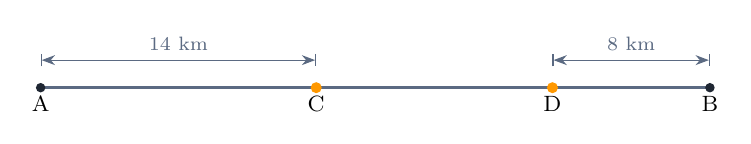
\begin{tikzpicture}[>=Stealth,font=\footnotesize]
\draw[line width=1.2pt,Slate] (0,0)--(8.5,0);
\foreach \x/\n in {0/A,8.5/B}{\fill[Ink] (\x,0) circle(0.06); \node[lbl,below] at (\x,-0.05){\n};}
\fill[tmOrange] (3.5,0) circle(0.07); \node[lbl,below] at (3.5,-0.05){C};
\fill[tmOrange] (6.5,0) circle(0.07); \node[lbl,below] at (6.5,-0.05){D};
\draw[|<->|,Slate] (0,0.35)--node[above,dim]{$14$ km}(3.5,0.35);
\draw[|<->|,Slate] (6.5,0.35)--node[above,dim]{$8$ km}(8.5,0.35);
\end{tikzpicture}
\end{center}
Đến lần gặp thứ nhất, cả hai bạn đi được một lần quãng đường AB; bạn đi từ A đi được $14$ km.\par
Đến lần gặp thứ hai, cả hai bạn đi được ba lần quãng đường AB, nên bạn đi từ A đi được $14\times3=42$ (km).\par
Bạn đó đã đi từ A đến B rồi quay lại $8$ km: $42=\text{AB}+8$, nên $\text{AB}=42-8=34$ (km).
\note{Thử lại: tỉ số vận tốc là $14:20$; bạn đi từ B đi được $20\times3=60=34+26$ km, tức là đến A rồi quay lại $26$ km, đúng tại chỗ cách B $8$ km.}
\dapso{$34$ km.}
\end{exbox}
\dividerbar{Luyện tập}
\begin{probbox}{1}{\relax}
Trên đường chạy dài $400$ m, hai vận động viên xuất phát cùng lúc, cùng một điểm và chạy ngược chiều nhau với vận tốc $4$ m/giây và $6$ m/giây. Hỏi sau bao lâu hai người gặp nhau lần thứ nhất?
\end{probbox}
\probsol{
Hai người cùng chạy được một vòng.\par Tổng vận tốc: $4+6=10$ (m/giây).\par Thời gian: $400:10=40$ (giây).
\dapso{$40$ giây.}}
\gap
\begin{probbox}{2}{\relax}
Hai vận động viên ở Bài 1 (vận tốc $4$ m/giây và $6$ m/giây) xuất phát cùng lúc, cùng một điểm trên đường chạy $400$ m nhưng chạy cùng chiều. Hỏi sau bao lâu hai người gặp nhau lần thứ nhất?
\end{probbox}
\probsol{
Người chạy nhanh phải chạy hơn người kia đúng một vòng.\par Hiệu vận tốc: $6-4=2$ (m/giây).\par Thời gian: $400:2=200$ (giây) $=3$ phút $20$ giây.
\dapso{$3$ phút $20$ giây.}}
\gap
\begin{probbox}{3}{\relax}
Một con đường quanh hồ có chu vi $3$ km. Hai người đi xe đạp xuất phát cùng lúc, cùng một điểm, đi ngược chiều nhau với vận tốc $12$ km/giờ và $18$ km/giờ. Hỏi sau bao nhiêu phút hai người gặp nhau?
\end{probbox}
\probsol{
Tổng vận tốc: $12+18=30$ (km/giờ).\par Thời gian: $3:30=0{,}1$ (giờ) $=6$ phút.
\dapso{$6$ phút.}}
\gap
\begin{probbox}{4}{\relax}
Hai người đi xe đạp ở Bài 3 bây giờ đi cùng chiều quanh hồ có chu vi $3$ km. Hỏi sau bao lâu người đi nhanh đuổi kịp người kia lần thứ nhất?
\end{probbox}
\probsol{
Hiệu vận tốc: $18-12=6$ (km/giờ).\par Thời gian: $3:6=0{,}5$ (giờ) $=30$ phút.
\dapso{$30$ phút.}}
\gap
\begin{probbox}{5}{\relax}
Đường đi bộ trong công viên là một vòng khép kín dài $900$ m. Lan đi với vận tốc $60$ m/phút, Mai đi với vận tốc $90$ m/phút; hai bạn xuất phát cùng lúc từ cổng và đi cùng chiều. Hỏi sau bao lâu Mai đuổi kịp Lan lần thứ nhất, và khi đó mỗi bạn đã đi được mấy vòng?
\end{probbox}
\probsol{
Hiệu vận tốc: $90-60=30$ (m/phút).\par Thời gian: $900:30=30$ (phút).\par
Lan: $60\times30=1\,800$ m $=2$ vòng; Mai: $90\times30=2\,700$ m $=3$ vòng.
\dapso{sau $30$ phút; Lan $2$ vòng, Mai $3$ vòng.}}
\gap
\begin{probbox}{6}{\relax}
An chạy quanh đường chạy dài $800$ m với vận tốc $150$ m/phút trong $14$ phút. Hỏi An đã chạy được mấy vòng trọn vẹn, và phải chạy thêm bao nhiêu mét nữa mới hết vòng đang chạy?
\end{probbox}
\probsol{
Quãng đường: $150\times14=2\,100$ (m).\par $2\,100=2\times800+500$: $2$ vòng trọn vẹn và thêm $500$ m.\par
Để hết vòng thứ ba: $800-500=300$ (m).
\dapso{$2$ vòng trọn vẹn; còn $300$ m.}}
\gap
\begin{probbox}{7}{\relax}
Một đường đua xe đạp hình tròn có đường kính $50$ m. Một bạn nhỏ đạp xe $5$ vòng. Hỏi bạn đó đi được bao nhiêu mét?
\end{probbox}
\probsol{
Chu vi một vòng: $50\times3{,}14=157$ (m).\par $5$ vòng: $157\times5=785$ (m).
\dapso{$785$ m.}}
\gap
\begin{probbox}{8}{\relax}
Một đường chạy hình tròn có đường kính $100$ m. Hai bạn xuất phát cùng lúc, cùng một điểm và chạy ngược chiều nhau với vận tốc $3$ m/giây và $5$ m/giây. Hỏi sau bao lâu hai bạn gặp nhau?
\end{probbox}
\probsol{
Chu vi: $100\times3{,}14=314$ (m).\par Tổng vận tốc: $3+5=8$ (m/giây).\par Thời gian: $314:8=39{,}25$ (giây).
\dapso{$39{,}25$ giây.}}
\gap
\begin{probbox}{9}{\relax}
Hai người đi xe đạp cùng chiều quanh một vòng đua dài $2$ km với vận tốc $20$ km/giờ và $25$ km/giờ, xuất phát cùng lúc, cùng một điểm. Trong $2$ giờ, người đi nhanh vượt người đi chậm bao nhiêu lần?
\end{probbox}
\probsol{
Trong $2$ giờ, người đi nhanh đi hơn người kia $(25-20)\times2=10$ (km).\par Mỗi lần vượt ứng với đi hơn một vòng: $10:2=5$ (lần).
\dapso{$5$ lần.}}
\gap
\begin{probbox}{10}{\relax}
Hai người xuất phát cùng lúc, cùng một điểm trên đường chạy dài $500$ m và chạy ngược chiều nhau với vận tốc $3$ m/giây và $2$ m/giây. Trong $10$ phút, hai người gặp nhau bao nhiêu lần?
\end{probbox}
\probsol{
Cứ $500:(3+2)=100$ (giây) hai người gặp nhau một lần.\par $10$ phút $=600$ giây; $600:100=6$ (lần).
\dapso{$6$ lần.}}
\gap
\begin{probbox}{11}{\relax}
Hai bạn chạy cùng chiều quanh một vòng dài $1$ km, xuất phát cùng lúc, cùng một điểm. Bạn chạy nhanh có vận tốc $250$ m/phút và đuổi kịp bạn kia lần thứ nhất sau $10$ phút. Tính vận tốc của bạn chạy chậm.
\end{probbox}
\probsol{
Hiệu vận tốc: $1\,000:10=100$ (m/phút).\par Vận tốc bạn chạy chậm: $250-100=150$ (m/phút).
\dapso{$150$ m/phút.}}
\gap
\begin{probbox}{12}{\relax}
Hai bạn chạy ngược chiều quanh một vòng dài $600$ m, xuất phát cùng lúc, cùng một điểm và gặp nhau sau $2$ phút. Một bạn chạy với vận tốc $140$ m/phút. Tính vận tốc của bạn kia.
\end{probbox}
\probsol{
Tổng vận tốc: $600:2=300$ (m/phút).\par Vận tốc bạn kia: $300-140=160$ (m/phút).
\dapso{$160$ m/phút.}}
\gap
\begin{probbox}{13}{\relax}
Trên đường chạy dài $400$ m, Bảo xuất phát ở phía trước Khoa $100$ m và hai bạn chạy cùng chiều. Khoa chạy với vận tốc $5$ m/giây, Bảo chạy với vận tốc $3$ m/giây. Hỏi sau bao lâu Khoa đuổi kịp Bảo?
\end{probbox}
\probsol{
Khoa phải chạy hơn Bảo $100$ m.\par Hiệu vận tốc: $5-3=2$ (m/giây).\par Thời gian: $100:2=50$ (giây).
\dapso{$50$ giây.}}
\gap
\begin{probbox}{14}{\relax}
Hùng chạy một vòng sân hết $4$ phút, Việt chạy một vòng hết $6$ phút. Hai bạn xuất phát cùng lúc, cùng một điểm và chạy cùng chiều. Hỏi sau bao lâu Hùng đuổi kịp Việt lần thứ nhất?
\end{probbox}
\probsol{
Mỗi phút Hùng chạy được $\dfrac14$ vòng, Việt chạy được $\dfrac16$ vòng; Hùng chạy hơn Việt $\dfrac14-\dfrac16=\dfrac1{12}$ vòng.\par
Để chạy hơn một vòng: $1:\dfrac1{12}=12$ (phút).
\dapso{$12$ phút.}}
\gap
\begin{probbox}{15}{\relax}
Hùng và Việt (chạy một vòng hết $4$ phút và $6$ phút) bây giờ xuất phát cùng lúc và chạy ngược chiều nhau. Hỏi sau bao lâu hai bạn gặp nhau?
\end{probbox}
\probsol{
Mỗi phút cả hai bạn chạy được $\dfrac14+\dfrac16=\dfrac5{12}$ vòng.\par
Thời gian: $1:\dfrac5{12}=\dfrac{12}5=2{,}4$ (phút) $=2$ phút $24$ giây.
\dapso{$2$ phút $24$ giây.}}
\gap
\begin{probbox}{16}{\relax}
Một bạn chạy mỗi vòng hết $3$ phút, một bạn khác chạy mỗi vòng hết $5$ phút. Hai bạn xuất phát cùng lúc từ vạch xuất phát. Hỏi sau bao lâu thì lần đầu tiên cả hai bạn cùng có mặt ở vạch xuất phát?
\end{probbox}
\probsol{
Bạn thứ nhất ở vạch xuất phát sau $3;\ 6;\ 9;\ 12;\ 15;\ldots$ phút; bạn thứ hai sau $5;\ 10;\ 15;\ldots$ phút.\par
Số chung nhỏ nhất: $15$.
\dapso{$15$ phút.}}
\gap
\begin{probbox}{17}{\relax}
Một vận động viên chạy $5$ vòng đường chạy dài $400$ m hết $10$ phút. Tính vận tốc của người đó theo m/phút và km/giờ.
\end{probbox}
\probsol{
Quãng đường: $400\times5=2\,000$ (m).\par Vận tốc: $2\,000:10=200$ (m/phút).\par $200$ m/phút $=12\,000$ m/giờ $=12$ km/giờ.
\dapso{$200$ m/phút $=12$ km/giờ.}}
\gap
\begin{probbox}{18}{\relax}
Quãng đường AB dài $30$ km. Một người đi xe đạp từ A đến B với vận tốc $12$ km/giờ, cùng lúc một người đi xe máy từ B về A với vận tốc $18$ km/giờ. Mỗi người đến đầu kia thì quay lại ngay.
\begin{cols2}
\pa{a} Lần gặp thứ nhất cách A bao nhiêu ki-lô-mét? & \pa{b} Lần gặp thứ hai cách A bao nhiêu ki-lô-mét?
\end{cols2}
\end{probbox}
\probsol{
\pa{a} Thời gian: $30:(12+18)=1$ (giờ); chỗ gặp cách A: $12\times1=12$ (km).\par
\pa{b} Đến lần gặp thứ hai, cả hai đi được $3\times30=90$ (km), hết $3$ giờ.\par
Người đi xe đạp đi được $12\times3=36$ (km) $=30+6$: đến B rồi quay lại $6$ km, tức là cách A $30-6=24$ (km).
\dapso{\pa{a} $12$ km;\quad \pa{b} $24$ km.}}
\gap
\begin{probbox}{19}{\relax}
Cùng một lúc, hai người đi từ A và từ B ngược chiều về phía nhau và gặp nhau lần thứ nhất ở chỗ cách A $9$ km. Mỗi người đi tiếp đến đầu kia rồi quay lại ngay; hai người gặp nhau lần thứ hai ở chỗ cách B $5$ km. Tính quãng đường AB.
\end{probbox}
\probsol{
Đến lần gặp thứ hai, người đi từ A đã đi được $9\times3=27$ (km).\par
Đó là quãng đường AB cộng $5$ km quay lại từ B: $\text{AB}=27-5=22$ (km).
\dapso{$22$ km.}}
\gap
\begin{probbox}{20}{\relax}
Hoa đi từ A, Quế đi từ B ngược chiều về phía nhau rồi cứ đi đi lại lại giữa A và B không nghỉ. Tỉ số vận tốc của Hoa và Quế là $2:3$. Khoảng cách giữa hai chỗ gặp nhau đầu tiên là $24$ m. Tính quãng đường AB.
\end{probbox}
\probsol{
Lần gặp thứ nhất: Hoa đi được $\dfrac25$ quãng đường AB.\par
Lần gặp thứ hai: Hoa đi được $3\times\dfrac25=\dfrac65$ quãng đường AB, tức là đến B rồi quay lại $\dfrac15$ AB: chỗ gặp cách A $\dfrac45$ AB.\par
Khoảng cách hai chỗ gặp: $\dfrac45-\dfrac25=\dfrac25$ AB $=24$ m; AB $=24:\dfrac25=60$ (m).
\dapso{$60$ m.}}
\gap
\begin{probbox}{21}{\relax}
Bánh xe đạp có đường kính $0{,}6$ m. Hỏi khi xe đi được $942$ m thì bánh xe quay được bao nhiêu vòng?
\end{probbox}
\probsol{
Mỗi vòng bánh xe đi được: $0{,}6\times3{,}14=1{,}884$ (m).\par Số vòng: $942:1{,}884=500$ (vòng).
\dapso{$500$ vòng.}}
\gap
\begin{probbox}{22}{\relax}
Kim phút của một chiếc đồng hồ dài $10$ cm. Hỏi đầu kim phút đi được bao nhiêu xăng-ti-mét trong $1$ giờ? Trong $3$ giờ?
\end{probbox}
\probsol{
Trong $1$ giờ đầu kim đi hết một vòng tròn bán kính $10$ cm: $10\times2\times3{,}14=62{,}8$ (cm).\par
Trong $3$ giờ: $62{,}8\times3=188{,}4$ (cm).
\dapso{$62{,}8$ cm; $188{,}4$ cm.}}
\gap
\begin{probbox}{23}{\relax}
Trên đường chạy dài $400$ m, A chạy với vận tốc $6$ m/giây, B chạy với vận tốc $4$ m/giây, cùng chiều, xuất phát cùng lúc, cùng một điểm. Khi A bắt vòng B lần thứ nhất thì A đã chạy được bao nhiêu mét, bao nhiêu vòng?
\end{probbox}
\probsol{
Thời gian: $400:(6-4)=200$ (giây).\par A chạy được $6\times200=1\,200$ (m) $=3$ vòng.
\dapso{$1\,200$ m, $3$ vòng.}}
\gap
\begin{probbox}{24}{\relax}
Phúc chạy một vòng sân hết $80$ giây, Long chạy một vòng hết $120$ giây. Hai bạn xuất phát cùng lúc, cùng một điểm và chạy ngược chiều nhau. Hỏi sau bao lâu hai bạn gặp nhau?
\end{probbox}
\probsol{
Mỗi giây cả hai bạn chạy được $\dfrac1{80}+\dfrac1{120}=\dfrac3{240}+\dfrac2{240}=\dfrac1{48}$ vòng.\par Thời gian: $48$ giây.
\dapso{$48$ giây.}}
\gap
\begin{probbox}{25}{\relax}
Hai con ngựa phi cùng chiều quanh một trường đua dài $1{,}2$ km với vận tốc $15$ m/giây và $12$ m/giây, xuất phát cùng lúc, cùng một điểm. Hỏi sau bao lâu con ngựa nhanh đuổi kịp con kia lần thứ nhất?
\end{probbox}
\probsol{
$1{,}2$ km $=1\,200$ m.\par Hiệu vận tốc: $3$ m/giây.\par Thời gian: $1\,200:3=400$ (giây) $=6$ phút $40$ giây.
\dapso{$6$ phút $40$ giây.}}
\gap
\begin{probbox}{26}{\relax}
Hai đoàn tàu đồ chơi chạy ngược chiều nhau trên một đường ray hình tròn dài $3$ m với vận tốc $0{,}25$ m/giây và $0{,}35$ m/giây, xuất phát từ cùng một điểm. Hỏi sau bao lâu hai tàu gặp nhau?
\end{probbox}
\probsol{
Tổng vận tốc: $0{,}25+0{,}35=0{,}6$ (m/giây).\par Thời gian: $3:0{,}6=5$ (giây).
\dapso{$5$ giây.}}
\gap
\begin{probbox}{27}{\relax}
Hai bạn xuất phát cùng lúc, cùng một điểm và chạy ngược chiều nhau quanh một đường chạy với vận tốc $4$ m/giây và $6$ m/giây. Hai bạn gặp nhau sau $40$ giây. Tính chiều dài đường chạy.
\end{probbox}
\probsol{
Trong $40$ giây cả hai chạy được một vòng: $(4+6)\times40=400$ (m).
\dapso{$400$ m.}}
\gap
\begin{probbox}{28}{\relax}
Hai người đi xe đạp xuất phát cùng lúc, cùng một điểm, đi cùng chiều quanh một vòng đường với vận tốc $260$ m/phút và $180$ m/phút. Người đi nhanh đuổi kịp người đi chậm lần thứ nhất sau $6$ phút. Tính chiều dài vòng đường.
\end{probbox}
\probsol{
Trong $6$ phút người đi nhanh đi hơn người kia một vòng: $(260-180)\times6=480$ (m).
\dapso{$480$ m.}}
\gap
\begin{probbox}{29}{\relax}
Ngân chạy từ nhà quanh một vòng đường dài $2{,}5$ km với vận tốc $9$ km/giờ trong $1$ giờ. Hỏi Ngân còn phải chạy tiếp (theo chiều cũ) bao xa nữa mới về đến nhà?
\end{probbox}
\probsol{
Quãng đường: $9$ km $=3\times2{,}5+1{,}5$: $3$ vòng và thêm $1{,}5$ km.\par
Còn phải chạy: $2{,}5-1{,}5=1$ (km).
\dapso{$1$ km.}}
\gap
\begin{probbox}{30}{\relax}
Hai bạn cùng lúc bơi từ hai đầu một bể bơi dài $50$ m, bơi đi bơi lại với vận tốc $1$ m/giây và $1{,}5$ m/giây, đến thành bể thì quay lại ngay. Hỏi sau bao lâu hai bạn gặp nhau lần thứ nhất? Lần thứ hai?
\end{probbox}
\probsol{
Lần thứ nhất: cả hai bơi được một chiều dài bể: $50:(1+1{,}5)=20$ (giây).\par
Lần thứ hai: cả hai bơi được ba chiều dài bể: $20\times3=60$ (giây).
\dapso{$20$ giây và $60$ giây.}}
\dividerbar{Thử thách -- Nâng cao}
\begin{probbox}{31}{\stars{1}}
Ba bạn chạy cùng chiều quanh đường chạy dài $300$ m với vận tốc $3$ m/giây, $4$ m/giây và $5$ m/giây, xuất phát cùng lúc, cùng một điểm. Hỏi sau bao lâu cả ba bạn lần đầu tiên lại gặp nhau?
\end{probbox}
\probsol{
Bạn $4$ m/giây và bạn $3$ m/giây gặp nhau sau mỗi $300:1=300$ (giây); bạn $5$ m/giây và bạn $4$ m/giây cũng sau mỗi $300$ giây; bạn $5$ m/giây và bạn $3$ m/giây sau mỗi $300:2=150$ (giây).\par
Cả ba gặp nhau khi từng cặp đều gặp nhau: lần đầu sau $300$ giây $=5$ phút.\par
(\emph{Thử lại:} ba bạn chạy được $900$ m, $1\,200$ m, $1\,500$ m, tức là $3$; $4$; $5$ vòng trọn vẹn.)
\dapso{$5$ phút.}}
\gap
\begin{probbox}{32}{\stars{1}}
Trên đường chạy dài $400$ m, hai bạn xuất phát cùng lúc, cùng một điểm, chạy cùng chiều với vận tốc $4$ m/giây và $5$ m/giây. Hỏi sau bao lâu thì lần đầu tiên cả hai cùng có mặt ở vạch xuất phát? Đó có phải là lần đầu tiên hai bạn gặp nhau không?
\end{probbox}
\probsol{
Thời gian chạy một vòng: $400:4=100$ (giây) và $400:5=80$ (giây). Cùng ở vạch xuất phát: bội chung nhỏ nhất của $100$ và $80$ là $400$ giây.\par
Hai bạn gặp nhau lần đầu khi bạn nhanh chạy hơn một vòng: $400:(5-4)=400$ (giây), nên đúng vậy, lần gặp đầu tiên ở ngay vạch xuất phát.
\dapso{$400$ giây $=6$ phút $40$ giây; có.}}
\gap
\begin{probbox}{33}{\stars{2}}
Trên đường chạy dài $400$ m, hai bạn xuất phát cùng lúc từ điểm S và chạy ngược chiều nhau với vận tốc $3$ m/giây và $5$ m/giây. Hỏi đến lần gặp nhau thứ mấy thì lần đầu tiên hai bạn gặp lại nhau đúng tại S, và vào lúc nào?
\end{probbox}
\probsol{
Cứ $400:8=50$ (giây) hai bạn gặp nhau một lần; giữa hai lần gặp, bạn chạy chậm chạy được $150$ m.\par
Các chỗ gặp nhau, đo từ S theo chiều chạy của bạn chậm: $150;\ 300;\ 50;\ 200;\ 350;\ 100;\ 250;\ 0$ (m).\par
Vậy lần gặp thứ $8$ ở đúng S, sau $8\times50=400$ (giây). (Khi đó bạn chạy chậm đã chạy $1\,200$ m $=3$ vòng.)
\dapso{lần gặp thứ $8$, sau $400$ giây.}}
\gap
\begin{probbox}{34}{\stars{2}}
Lúc đúng $3$ giờ, hỏi sau bao nhiêu phút thì kim giờ và kim phút trùng nhau lần đầu tiên?
\end{probbox}
\probsol{
Lúc $3$ giờ, kim phút ở sau kim giờ $15$ vạch chia phút.\par
Mỗi phút kim phút đi hơn kim giờ $1-\dfrac1{12}=\dfrac{11}{12}$ vạch.\par
Thời gian: $15:\dfrac{11}{12}=\dfrac{180}{11}=16\dfrac4{11}$ (phút).
\dapso{$16\dfrac4{11}$ phút (khoảng $3$ giờ $16$ phút).}}
\gap
\begin{probbox}{35}{\stars{2}}
Từ sau $12$ giờ trưa đến $12$ giờ đêm (tính cả lúc $12$ giờ đêm), kim giờ và kim phút trùng nhau bao nhiêu lần?
\end{probbox}
\probsol{
Kim phút đi hơn kim giờ một vòng ($60$ vạch) sau mỗi $60:\dfrac{11}{12}=\dfrac{720}{11}$ phút $=\dfrac{12}{11}$ giờ.\par
Trong $12$ giờ: $12:\dfrac{12}{11}=11$ (lần).
\dapso{$11$ lần.}}
\gap
\begin{probbox}{36}{\stars{1}}
Trên đường chạy dài $600$ m, B xuất phát ở phía trước A $200$ m, hai bạn chạy cùng chiều; A chạy với vận tốc $5$ m/giây, B chạy với vận tốc $3$ m/giây. Hỏi A đuổi kịp B lần thứ nhất sau bao lâu? Lần thứ hai sau bao lâu?
\end{probbox}
\probsol{
Lần thứ nhất: A phải chạy hơn B $200$ m: $200:2=100$ (giây).\par
Sau đó A phải chạy hơn B thêm một vòng: $600:2=300$ (giây); lần thứ hai: $100+300=400$ (giây).
\dapso{sau $100$ giây và sau $400$ giây.}}
\gap
\begin{probbox}{37}{\stars{1}}
Trên đường chạy dài $400$ m, hai bạn xuất phát cùng lúc, cùng một điểm. Nếu chạy ngược chiều thì sau $40$ giây gặp nhau, nếu chạy cùng chiều thì sau $200$ giây gặp nhau. Tính vận tốc mỗi bạn.
\end{probbox}
\probsol{
Tổng vận tốc: $400:40=10$ (m/giây); hiệu vận tốc: $400:200=2$ (m/giây).\par
Bạn chạy nhanh: $(10+2):2=6$ (m/giây); bạn chạy chậm: $10-6=4$ (m/giây).
\dapso{$6$ m/giây và $4$ m/giây.}}
\gap
\begin{probbox}{38}{\stars{2}}
Yến chạy một vòng sân hết $6$ phút. Yến và Xuân xuất phát cùng một điểm, chạy ngược chiều nhau thì cứ $2$ phút $24$ giây lại gặp nhau một lần. Hỏi Xuân chạy một vòng sân hết bao lâu?
\end{probbox}
\probsol{
$2$ phút $24$ giây $=2{,}4$ phút; mỗi phút cả hai chạy được $1:2{,}4=\dfrac5{12}$ vòng.\par
Xuân: $\dfrac5{12}-\dfrac16=\dfrac3{12}=\dfrac14$ vòng mỗi phút, nên một vòng hết $4$ phút.
\dapso{$4$ phút.}}
\gap
\begin{probbox}{39}{\stars{2}}
Hai người bạn ở cách nhau $6$ km, đi ngược chiều về phía nhau với vận tốc $3$ km/giờ và $5$ km/giờ. Một chú chó xuất phát cùng người thứ nhất, chạy với vận tốc $12$ km/giờ đi đi lại lại giữa hai người cho đến khi hai người gặp nhau. Hỏi chú chó đã chạy được bao nhiêu ki-lô-mét?
\end{probbox}
\probsol{
Hai người gặp nhau sau $6:(3+5)=0{,}75$ (giờ).\par Chú chó chạy suốt thời gian đó: $12\times0{,}75=9$ (km).
\dapso{$9$ km.}}
\gap
\begin{probbox}{40}{\stars{2}}
Hà đi bộ từ A đến B rồi quay lại A, cứ đi đi lại lại như vậy; cùng lúc đó Tú đi từ B đến A rồi quay lại B, cũng đi đi lại lại như vậy. Vận tốc của Hà bằng $80\%$ vận tốc của Tú. Khoảng cách giữa hai chỗ gặp nhau đầu tiên là $40$ m. Tính quãng đường AB.
\end{probbox}
\probsol{
Tỉ số vận tốc Hà $:$ Tú $=4:5$. Lần gặp thứ nhất: Hà đi được $\dfrac49$ quãng đường AB.\par
Lần gặp thứ hai: Hà đi được $3\times\dfrac49=\dfrac{12}9$ quãng đường AB: đến B rồi quay lại $\dfrac39$ AB, nên chỗ gặp cách A $\dfrac69$ AB.\par
Khoảng cách: $\dfrac69-\dfrac49=\dfrac29$ AB $=40$ m; AB $=40:\dfrac29=180$ (m).
\dapso{$180$ m.}}
\gap
\begin{probbox}{41}{\stars{2}}
Hai ô tô cùng lúc khởi hành từ A và B đi ngược chiều về phía nhau, gặp nhau lần thứ nhất ở chỗ cách A $40$ km. Mỗi xe đi tiếp đến đầu kia rồi quay lại ngay; hai xe gặp nhau lần thứ hai ở chỗ cách A $20$ km. Tính quãng đường AB.
\end{probbox}
\probsol{
Đến lần gặp thứ hai, xe đi từ A đã đi được $40\times3=120$ (km).\par
Xe đó đi từ A đến B rồi quay lại đến chỗ cách A $20$ km: $120=\text{AB}+(\text{AB}-20)$.\par
Vậy $2\times\text{AB}=140$, $\text{AB}=70$ km.
\dapso{$70$ km.}}
\gap
\begin{probbox}{42}{\stars{1}}
Trên đường chạy dài $500$ m, Kiên (vận tốc $3$ m/giây) và Lâm (vận tốc $2$ m/giây) xuất phát cùng lúc từ S và chạy ngược chiều nhau. Hỏi hai bạn gặp nhau lần thứ ba vào lúc nào, ở chỗ cách S bao xa theo chiều chạy của Kiên?
\end{probbox}
\probsol{
Cứ $500:5=100$ (giây) hai bạn gặp nhau một lần; lần thứ ba sau $300$ giây.\par
Kiên đã chạy $3\times300=900$ (m) $=500+400$: cách S $400$ m theo chiều chạy của Kiên.
\dapso{sau $300$ giây ($5$ phút), cách S $400$ m.}}
\gap
\begin{probbox}{43}{\stars{1}}
Trên đường chạy dài $400$ m, A chạy với vận tốc $5$ m/giây, B chạy chậm hơn, cùng chiều, xuất phát cùng lúc, cùng một điểm. A bắt vòng B lần thứ nhất đúng lúc A chạy xong vòng thứ $5$. Tính vận tốc của B.
\end{probbox}
\probsol{
A chạy $5\times400=2\,000$ (m) hết $2\,000:5=400$ (giây).\par
B chạy ít hơn A một vòng: $1\,600$ m; vận tốc: $1\,600:400=4$ (m/giây).
\dapso{$4$ m/giây.}}
\gap
\begin{probbox}{44}{\stars{1}}
Trên đường chạy dài $400$ m, hai bạn xuất phát cùng lúc từ S, chạy ngược chiều nhau và gặp nhau ở chỗ cách S $160$ m theo chiều chạy của bạn thứ nhất. Bạn thứ nhất chạy với vận tốc $4$ m/giây. Tính vận tốc của bạn thứ hai.
\end{probbox}
\probsol{
Thời gian: $160:4=40$ (giây). Bạn thứ hai chạy phần còn lại của vòng: $400-160=240$ (m).\par Vận tốc: $240:40=6$ (m/giây).
\dapso{$6$ m/giây.}}
\gap
\begin{probbox}{45}{\stars{1}}
Một vòng đu quay có đường kính $40$ m, cứ $8$ phút quay được một vòng. Hỏi mỗi cabin trên vành đu quay chuyển động với vận tốc bao nhiêu mét mỗi phút?
\end{probbox}
\probsol{
Một vòng: $40\times3{,}14=125{,}6$ (m).\par Vận tốc: $125{,}6:8=15{,}7$ (m/phút).
\dapso{$15{,}7$ m/phút.}}
\gap
\begin{probbox}{46}{\stars{1}}
Bánh xe đạp có đường kính $0{,}5$ m, mỗi phút quay được $200$ vòng. Tính vận tốc của xe đạp theo km/giờ.
\end{probbox}
\probsol{
Mỗi vòng: $0{,}5\times3{,}14=1{,}57$ (m); mỗi phút: $1{,}57\times200=314$ (m).\par
Mỗi giờ: $314\times60=18\,840$ (m) $=18{,}84$ km.
\dapso{$18{,}84$ km/giờ.}}
\gap
\begin{probbox}{47}{\stars{1}}
Hai bạn cùng lúc xuất phát từ hai điểm đối diện nhau trên đường chạy dài $400$ m (cách nhau nửa vòng) và chạy cùng chiều với vận tốc $6$ m/giây và $4$ m/giây. Hỏi sau bao lâu bạn chạy nhanh đuổi kịp bạn chạy chậm?
\end{probbox}
\probsol{
Bạn chạy nhanh ở phía sau bạn kia $400:2=200$ (m).\par Thời gian: $200:(6-4)=100$ (giây).
\dapso{$100$ giây.}}
\gap
\begin{probbox}{48}{\stars{2}}
Hai bạn cùng lúc xuất phát từ hai điểm đối diện nhau trên đường chạy dài $400$ m và chạy ngược chiều về phía nhau với vận tốc $3$ m/giây và $5$ m/giây. Hỏi hai bạn gặp nhau lần thứ ba vào lúc nào?
\end{probbox}
\probsol{
Lần thứ nhất: hai bạn đi hết khoảng cách $200$ m: $200:8=25$ (giây).\par Sau đó cứ $400:8=50$ (giây) gặp nhau một lần.\par
Lần thứ ba: $25+50\times2=125$ (giây).
\dapso{sau $125$ giây $=2$ phút $5$ giây.}}
\gap
\begin{probbox}{49}{\stars{1}}
Hai bạn đi từ hai đầu một con đường dài $1{,}2$ km về phía nhau với vận tốc $70$ m/phút và $50$ m/phút, rồi tiếp tục đi đi lại lại không nghỉ. Hỏi sau bao lâu kể từ lúc xuất phát hai bạn gặp nhau lần thứ hai?
\end{probbox}
\probsol{
Đến lần gặp thứ hai, cả hai đi được $3\times1\,200=3\,600$ (m).\par Thời gian: $3\,600:(70+50)=30$ (phút).
\dapso{$30$ phút.}}
\gap
\begin{probbox}{50}{\stars{2}}
Hai bạn xuất phát cùng lúc, cùng một điểm trên một đường chạy. Nếu chạy ngược chiều thì cứ $30$ giây gặp nhau một lần; nếu chạy cùng chiều thì cứ $2$ phút $30$ giây bạn nhanh lại bắt vòng bạn chậm một lần. Hỏi mỗi bạn chạy một vòng hết bao lâu?
\end{probbox}
\probsol{
$2$ phút $30$ giây $=150$ giây. Mỗi giây: tổng phần vòng hai bạn chạy được $=\dfrac1{30}=\dfrac5{150}$, hiệu $=\dfrac1{150}$.\par
Bạn nhanh: $\left(\dfrac5{150}+\dfrac1{150}\right):2=\dfrac3{150}=\dfrac1{50}$ vòng mỗi giây, nên một vòng hết $50$ giây.\par
Bạn chậm: $\dfrac5{150}-\dfrac3{150}=\dfrac2{150}=\dfrac1{75}$ vòng mỗi giây, nên một vòng hết $75$ giây.
\dapso{$50$ giây và $75$ giây.}}
\clearpage
\titlehead
\begingroup\setbox0=\vbox{\section*{Thống kê, xác suất}}\endgroup
\chapterhead{11}{Thống kê, xác suất}
\shead{Thu thập và biểu diễn số liệu}
% ---- chapter 11 helpers: bar chart, pie chart with legend, pictograph icons ----
\newcommand{\stpBars}[6]{% #1 cm per unit, #2 ymax, #3 ystep, #4 list name/height/shown, #5 y caption, #6 x caption
\begin{tikzpicture}[font=\footnotesize,y=#1cm,x=1cm,>=stealth]
\foreach \n/\v/\d [count=\i] in {#4}{\xdef\stpN{\i}}
\pgfmathsetmacro\stpW{\stpN*1.2+0.1}
\foreach \t in {0,#3,...,#2}{\draw[Line] (0,\t)--(\stpW,\t); \node[left,text=Slate] at (0,\t){$\t$};}
\foreach \n/\v/\d [count=\i] in {#4}{
  \pgfmathsetmacro\stpC{\i*1.2-0.5}
  \fill[tmBlue!65] (\stpC-0.3,0) rectangle (\stpC+0.3,\v);
  \node[above,font=\footnotesize\bfseries,text=Ink] at (\stpC,\v){$\d$};
  \node[below,text=Ink] at (\stpC,0){\n};}
\draw[->,line width=0.8pt] (0,0)--([yshift=0.55cm]0,#2);
\draw[->,line width=0.8pt] (0,0)--(\stpW+0.35,0);
\node[above,text=Slate] at ([yshift=0.55cm]0,#2){#5};
\node[right,text=Slate] at (\stpW+0.35,0){#6};
\end{tikzpicture}}
\newcommand{\stpPie}[2][1.5]{% #2 list value/text/colour/legend name (value in percent)
\begin{tikzpicture}[font=\footnotesize]
\def\stpA{90}
\foreach \v/\t/\c/\n [count=\i] in {#2}{
  \pgfmathsetmacro\stpB{\stpA-3.6*\v}
  \pgfmathsetmacro\stpM{(\stpA+\stpB)/2}
  \pgfmathsetmacro\stpR{0.64*#1}
  \fill[\c] (0,0) -- (\stpA:#1) arc[start angle=\stpA,end angle=\stpB,radius=#1] -- cycle;
  \draw[white,line width=1.2pt] (0,0) -- (\stpA:#1);
  \node[text=Ink,font=\footnotesize\bfseries] at (\stpM:\stpR) {\t};
  \fill[\c] (#1+0.7,#1-0.55*\i+0.1) rectangle ++(0.32,0.32);
  \node[anchor=west,text=Ink,font=\small] at (#1+1.1,#1-0.55*\i+0.26) {\n};
  \global\let\stpA\stpB}
\draw[Slate,line width=0.8pt] (0,0) circle (#1);
\end{tikzpicture}}
\newcommand{\stpIcons}[1]{\foreach \k in {1,...,#1}{\textcolor{tmBlue}{\faBook}\ }}
\begin{knowbox}
Để so sánh, đánh giá và đưa ra quyết định, người ta \textbf{thu thập thông tin} (số liệu) rồi \textbf{sắp xếp, xử lí} các số liệu đó. Có khi ta thu thập toàn bộ, có khi chỉ thu thập ở một nhóm có lựa chọn mang tính điển hình.\par\smallskip
Các hình thức biểu diễn số liệu thường dùng:
\begin{itemize}[leftmargin=1.4em,itemsep=3pt]
\item \textbf{bảng số liệu} -- mỗi số liệu được ghi vào một ô;
\item \textbf{biểu đồ tranh} -- mỗi hình vẽ biểu thị cùng một số lượng;
\item \textbf{biểu đồ cột} -- chiều cao mỗi cột, đọc theo vạch chia trên trục đứng, cho biết số liệu;
\item \textbf{biểu đồ hình quạt tròn} -- cả hình tròn biểu thị toàn bộ ($100\%$); mỗi hình quạt biểu thị một tỉ số phần trăm của toàn bộ. Nửa hình tròn là $50\%$, một phần tư hình tròn là $25\%$.
\end{itemize}
Với biểu đồ hình quạt: \quad \textbf{số phần $=$ tổng số $:100\times$ số phần trăm}; \quad \textbf{tổng số $=$ số phần $:$ số phần trăm $\times100$}.
\end{knowbox}
\shead{Số trung bình cộng}
\begin{knowbox}
\textbf{Số trung bình cộng} $=$ (tổng các số liệu) $:$ (số các số liệu). \qquad \textbf{Tổng} $=$ số trung bình cộng $\times$ số các số liệu.
\begin{itemize}[leftmargin=1.4em,itemsep=3pt]
\item Số trung bình cộng luôn nằm giữa số liệu bé nhất và số liệu lớn nhất.
\item Muốn tìm \emph{một số liệu chưa biết}: tính tổng từ số trung bình cộng, rồi trừ đi các số liệu đã biết.
\item Nếu một số liệu tăng thêm bao nhiêu thì tổng tăng thêm bấy nhiêu, còn số trung bình cộng tăng thêm (số đó) $:$ (số các số liệu).
\end{itemize}
\end{knowbox}
\shead{Khả năng xảy ra và đếm các kết quả}
\begin{knowbox}
Khi thực hiện lặp lại một hoạt động (tung đồng xu, gieo xúc xắc, quay vòng quay, lấy bóng mà không nhìn), ta ghi lại số lần xuất hiện của mỗi khả năng.
\begin{center}
\textbf{tỉ số mô tả số lần lặp lại của một khả năng} $=$ $\dfrac{\text{số lần khả năng đó xảy ra}}{\text{tổng số lần thực hiện}}$
\end{center}
Ví dụ: gieo xúc xắc $20$ lần, mặt $6$ chấm xuất hiện $3$ lần thì tỉ số đó là $\dfrac{3}{20}$. Nếu gieo thêm nhiều lần, tỉ số này có thể thay đổi.\par\smallskip
\textbf{Đếm các kết quả.} Liệt kê có thứ tự mọi kết quả có thể (bằng danh sách, bảng hoặc sơ đồ cây). Đồng xu có $2$ kết quả, xúc xắc có $6$ kết quả; tung một đồng xu \emph{và} gieo một xúc xắc thì có $2\times6=12$ kết quả.\par
Khi các kết quả có \emph{khả năng như nhau}, \textbf{khả năng xảy ra} của một sự kiện $=$ (số kết quả làm sự kiện xảy ra) $:$ (số tất cả các kết quả). Sự kiện luôn xảy ra là \emph{chắc chắn}; sự kiện không bao giờ xảy ra là \emph{không thể}.
\end{knowbox}
\gap
\begin{exbox}{\ExWord\ 1}
Lan ghi lại số trang sách mình đọc mỗi ngày trong một tuần:
\begin{center}
\begin{tabular}{|l|c|c|c|c|c|c|c|}
\hline
\textbf{Thứ} & Hai & Ba & Tư & Năm & Sáu & Bảy & CN\\\hline
\textbf{Số trang} & $18$ & $25$ & $20$ & $32$ & $15$ & $30$ & $28$\\\hline
\end{tabular}
\end{center}
\begin{cols2}
\pa{a} Ngày nào Lan đọc nhiều nhất? Ít nhất? & \pa{b} Trung bình mỗi ngày Lan đọc bao nhiêu trang?\\
\multicolumn{2}{@{}l@{}}{\pa{c} Có bao nhiêu ngày Lan đọc nhiều hơn số trang trung bình?}
\end{cols2}
\guide
\pa{a} Nhiều nhất vào thứ Năm ($32$ trang); ít nhất vào thứ Sáu ($15$ trang).\par
\pa{b} Số trang đọc trong tuần: $18+25+20+32+15+30+28=168$ (trang).\par Trung bình mỗi ngày: $168:7=24$ (trang).\par
\pa{c} Nhiều hơn $24$ trang: thứ Ba, thứ Năm, thứ Bảy và Chủ nhật, tức là $4$ ngày.
\dapso{\pa{a} Thứ Năm; thứ Sáu. \pa{b} $24$ trang. \pa{c} $4$ ngày.}
\end{exbox}
\gap
\begin{exbox}{\ExWord\ 2}
Biểu đồ cột dưới đây cho biết số sách năm lớp quyên góp cho thư viện trường.
\begin{center}
\stpBars{0.05}{80}{10}{5A/45/45,5B/60/60,5C/35/35,5D/70/70,5E/40/40}{(quyển)}{(lớp)}
\end{center}
\begin{cols2}
\pa{a} Cả năm lớp quyên góp được bao nhiêu quyển sách? & \pa{b} Trung bình mỗi lớp quyên góp bao nhiêu quyển?\\
\multicolumn{2}{@{}l@{}}{\pa{c} Lớp góp nhiều nhất hơn lớp góp ít nhất bao nhiêu quyển sách?}
\end{cols2}
\guide
\pa{a} $45+60+35+70+40=250$ (quyển).\par
\pa{b} $250:5=50$ (quyển).\par
\pa{c} Nhiều nhất: lớp 5D ($70$ quyển); ít nhất: lớp 5C ($35$ quyển).\par Hơn nhau: $70-35=35$ (quyển).
\dapso{\pa{a} $250$ quyển. \pa{b} $50$ quyển. \pa{c} $35$ quyển.}
\end{exbox}
\gap
\begin{exbox}{\ExWord\ 3}
Khảo sát $400$ học sinh về loại quả yêu thích nhất, kết quả được cho trong biểu đồ hình quạt tròn.
\begin{center}
\stpPie{35/35\%/tmBlue!55/Xoài,20/20\%/tmOrange!60/Chuối,25/25\%/tmGreen!50/Dưa hấu,20/?/tmPurple!40/Cam}
\end{center}
\pa{a} Có bao nhiêu phần trăm học sinh chọn cam?\par
\pa{b} Có bao nhiêu học sinh chọn xoài?\par
\pa{c} Số học sinh chọn xoài nhiều hơn số học sinh chọn chuối bao nhiêu bạn?
\guide
\pa{a} Cả hình tròn là $100\%$: $100\%-35\%-20\%-25\%=20\%$.\par
\pa{b} $400:100\times35=140$ (học sinh).\par
\pa{c} \emph{Cách 1.} Số học sinh chọn chuối: $400:100\times20=80$ (học sinh); \ $140-80=60$ (học sinh).\par
\emph{Cách 2.} Chọn xoài nhiều hơn chọn chuối $35\%-20\%=15\%$; \ $400:100\times15=60$ (học sinh).
\dapso{\pa{a} $20\%$. \pa{b} $140$ học sinh. \pa{c} $60$ học sinh.}
\end{exbox}
\gap
\begin{exbox}{\ExWord\ 4}
Minh gieo một con xúc xắc $40$ lần và ghi lại kết quả.
\begin{center}
\begin{tabular}{|l|c|c|c|c|c|c|}
\hline
\textbf{Khả năng} & $1$ chấm & $2$ chấm & $3$ chấm & $4$ chấm & $5$ chấm & $6$ chấm\\\hline
\textbf{Số lần} & $6$ & $8$ & $5$ & $7$ & $9$ & $5$\\\hline
\end{tabular}
\end{center}
Viết tỉ số mô tả số lần lặp lại của mỗi khả năng sau so với tổng số lần gieo:\par
\pa{a} mặt $6$ chấm; \quad \pa{b} mặt có số chấm chẵn; \quad \pa{c} mặt có ít nhất $5$ chấm.
\guide
\pa{a} Mặt $6$ chấm xuất hiện $5$ lần: $\dfrac{5}{40}=\dfrac{1}{8}$.\par
\pa{b} Số chấm chẵn ($2$, $4$, $6$ chấm): $8+7+5=20$ (lần); \ $\dfrac{20}{40}=\dfrac12$.\par
\pa{c} Ít nhất $5$ chấm ($5$ hoặc $6$ chấm): $9+5=14$ (lần); \ $\dfrac{14}{40}=\dfrac{7}{20}$.
\note{Điều này không có nghĩa là lần sau cũng xảy ra như vậy: gieo càng nhiều lần thì các tỉ số này càng thay đổi.}
\dapso{\pa{a} $\dfrac18$. \pa{b} $\dfrac12$. \pa{c} $\dfrac{7}{20}$.}
\end{exbox}
\gap
\begin{exbox}{\ExWord\ 5}
Hộp I có ba tấm thẻ ghi số $1$, $2$, $3$; hộp II có hai tấm thẻ ghi số $4$, $5$. Không nhìn vào hộp, Hoa lấy ở mỗi hộp một tấm thẻ rồi cộng hai số trên thẻ.\par
\pa{a} Liệt kê tất cả các kết quả có thể. \quad \pa{b} Khả năng tổng bằng $7$ là bao nhiêu?
\guide
\pa{a} Lập bảng (hàng: thẻ hộp I, cột: thẻ hộp II):
\begin{center}
\begin{tabular}{|c|c|c|}
\hline
$+$ & $4$ & $5$\\\hline
$1$ & $5$ & $6$\\\hline
$2$ & $6$ & $7$\\\hline
$3$ & $7$ & $8$\\\hline
\end{tabular}
\end{center}
Có $3\times2=6$ kết quả có khả năng như nhau: $1+4;\ 1+5;\ 2+4;\ 2+5;\ 3+4;\ 3+5$.\par
\pa{b} Tổng bằng $7$ ở $2$ kết quả ($2+5$ và $3+4$).\par Khả năng: $\dfrac26=\dfrac13$.
\dapso{\pa{a} $6$ kết quả. \pa{b} $\dfrac13$.}
\end{exbox}
\dividerbar{Luyện tập}
\needspace{5cm}
\begin{probbox}{1}{\relax}
Nhiệt độ lúc giữa trưa ở một thị trấn trong năm ngày như sau:
\begin{center}
\begin{tabular}{|l|c|c|c|c|c|}
\hline
\textbf{Thứ} & Hai & Ba & Tư & Năm & Sáu\\\hline
\textbf{Nhiệt độ ($^\circ$C)} & $31$ & $29$ & $33$ & $30$ & $32$\\\hline
\end{tabular}
\end{center}
\pa{a} Ngày nào nóng nhất, ngày nào mát nhất? \quad \pa{b} Tính nhiệt độ trung bình lúc giữa trưa.
\end{probbox}
\probsol{
\pa{a} Nóng nhất: thứ Tư ($33^\circ$C); mát nhất: thứ Ba ($29^\circ$C).\par
\pa{b} $(31+29+33+30+32):5=155:5=31\ (^\circ\text{C})$.
\dapso{\pa{a} Thứ Tư; thứ Ba. \pa{b} $31^\circ$C.}}
\gap
\begin{probbox}{2}{\relax}
Điểm sáu bài kiểm tra Toán của Nam là $7;\ 9;\ 8;\ 10;\ 6;\ 8$. Tính điểm trung bình của Nam.
\end{probbox}
\probsol{
Tổng điểm: $7+9+8+10+6+8=48$.\par Điểm trung bình: $48:6=8$.
\dapso{$8$ điểm.}}
\gap
\begin{probbox}{3}{\relax}
Bốn bạn cao $135$ cm, $142$ cm, $138$ cm và $145$ cm. Tính chiều cao trung bình của bốn bạn.
\end{probbox}
\probsol{
$(135+142+138+145):4=560:4=140$ (cm).
\dapso{$140$ cm.}}
\gap
\needspace{5cm}
\begin{probbox}{4}{\relax}
Biểu đồ tranh dưới đây cho biết số sách bốn tổ đã đọc trong tháng Năm.
\begin{center}
\begin{tabular}{|l|l|}
\hline
Tổ 1 & \stpIcons{5}\\\hline
Tổ 2 & \stpIcons{3}\\\hline
Tổ 3 & \stpIcons{6}\\\hline
Tổ 4 & \stpIcons{4}\\\hline
\end{tabular}\par\smallskip
Mỗi \textcolor{tmBlue}{\faBook} chỉ $4$ quyển sách.
\end{center}
\pa{a} Cả bốn tổ đọc được bao nhiêu quyển sách? \quad \pa{b} Trung bình mỗi tổ đọc bao nhiêu quyển?
\end{probbox}
\probsol{
Số hình vẽ: $5+3+6+4=18$ (hình).\par
\pa{a} Số sách: $4\times18=72$ (quyển).\par
\pa{b} Trung bình: $72:4=18$ (quyển).
\dapso{\pa{a} $72$ quyển. \pa{b} $18$ quyển.}}
\gap
\begin{probbox}{5}{\relax}
Một cửa hàng bán được $24$ chiếc xe đạp trong tháng Một, $30$ chiếc trong tháng Hai, $27$ chiếc trong tháng Ba và $39$ chiếc trong tháng Tư.\par
\pa{a} Bốn tháng cửa hàng bán được bao nhiêu chiếc xe đạp? \quad \pa{b} Trung bình mỗi tháng bán được bao nhiêu chiếc?\par
\pa{c} Có mấy tháng cửa hàng bán được nhiều hơn mức trung bình?
\end{probbox}
\probsol{
\pa{a} $24+30+27+39=120$ (chiếc).\par
\pa{b} $120:4=30$ (chiếc).\par
\pa{c} Chỉ có tháng Tư ($39>30$; tháng Hai bán $30$ chiếc, bằng mức trung bình chứ không nhiều hơn): $1$ tháng.
\dapso{\pa{a} $120$ chiếc. \pa{b} $30$ chiếc. \pa{c} $1$ tháng.}}
\gap
\needspace{8.5cm}
\begin{probbox}{6}{\relax}
Biểu đồ cho biết số học sinh mỗi khối của một trường tiểu học.
\begin{center}
\stpBars{0.025}{150}{25}{Khối 1/120/120,Khối 2/135/135,Khối 3/110/110,Khối 4/140/140,Khối 5/125/125}{(học sinh)}{}
\end{center}
\pa{a} Khối nào có nhiều học sinh nhất? Ít học sinh nhất?\par
\pa{b} Trường có tất cả bao nhiêu học sinh?\par
\pa{c} Khối 4 nhiều hơn khối 3 bao nhiêu học sinh?
\end{probbox}
\probsol{
\pa{a} Nhiều nhất: khối 4 ($140$ học sinh); ít nhất: khối 3 ($110$ học sinh).\par
\pa{b} $120+135+110+140+125=630$ (học sinh).\par
\pa{c} $140-110=30$ (học sinh).
\dapso{\pa{a} Khối 4; khối 3. \pa{b} $630$ học sinh. \pa{c} $30$ học sinh.}}
\gap
\needspace{8.5cm}
\begin{probbox}{7}{\relax}
Biểu đồ cho biết lượng mưa ở một thị trấn từ tháng Năm đến tháng Tám.
\begin{center}
\stpBars{0.014}{250}{50}{Tháng 5/80/80,Tháng 6/150/150,Tháng 7/210/210,Tháng 8/120/120}{(mm)}{}
\end{center}
Tính tổng lượng mưa và lượng mưa trung bình mỗi tháng.
\end{probbox}
\probsol{
Tổng lượng mưa: $80+150+210+120=560$ (mm).\par Trung bình mỗi tháng: $560:4=140$ (mm).
\dapso{$560$ mm; $140$ mm.}}
\gap
\needspace{7.5cm}
\begin{probbox}{8}{\relax}
Lớp 5B có $40$ học sinh. Biểu đồ hình quạt tròn cho biết cách các bạn đến trường.
\begin{center}
\stpPie{30/30\%/tmBlue!55/Đi bộ,45/45\%/tmOrange!60/Đi xe đạp,25/25\%/tmGreen!50/Bố mẹ đưa bằng xe máy}
\end{center}
\pa{a} Có bao nhiêu học sinh đi bộ đến trường?\par
\pa{b} Số học sinh đi xe đạp nhiều hơn số học sinh được đưa bằng xe máy bao nhiêu bạn?
\end{probbox}
\probsol{
\pa{a} $40:100\times30=12$ (học sinh).\par
\pa{b} Đi xe đạp: $40:100\times45=18$ (học sinh); đi xe máy: $40:100\times25=10$ (học sinh).\par Nhiều hơn: $18-10=8$ (học sinh).
\dapso{\pa{a} $12$ học sinh. \pa{b} $8$ học sinh.}}
\gap
\needspace{7.5cm}
\begin{probbox}{9}{\relax}
$200$ học sinh chọn môn thể thao yêu thích nhất của mình.
\begin{center}
\stpPie{40/40\%/tmBlue!55/Bóng đá,25/25\%/tmOrange!60/Cầu lông,20/20\%/tmGreen!50/Bơi,15/15\%/tmPurple!40/Cờ vua}
\end{center}
\pa{a} Có bao nhiêu học sinh chọn bóng đá? \quad \pa{b} chọn cờ vua?\par
\pa{c} Có bao nhiêu học sinh chọn bóng đá hoặc bơi?
\end{probbox}
\probsol{
\pa{a} $200:100\times40=80$ (học sinh).\par
\pa{b} $200:100\times15=30$ (học sinh).\par
\pa{c} $40\%+20\%=60\%$; \ $200:100\times60=120$ (học sinh).
\dapso{\pa{a} $80$. \pa{b} $30$. \pa{c} $120$ học sinh.}}
\gap
\needspace{7.5cm}
\begin{probbox}{10}{\relax}
$300$ học sinh, mỗi bạn tham gia một câu lạc bộ sau giờ học.
\begin{center}
\stpPie{30/30\%/tmBlue!55/Mĩ thuật,25/25\%/tmOrange!60/Âm nhạc,25/?/tmGreen!50/Khoa học,20/20\%/tmPurple!40/Thể thao}
\end{center}
Có bao nhiêu phần trăm học sinh tham gia câu lạc bộ Khoa học và đó là bao nhiêu học sinh?
\end{probbox}
\probsol{
Khoa học: $100\%-30\%-25\%-20\%=25\%$.\par Số học sinh: $300:100\times25=75$ (học sinh).
\dapso{$25\%$; $75$ học sinh.}}
\gap
\needspace{7.5cm}
\begin{probbox}{11}{\relax}
Một gia đình chi tiêu $12\,000\,000$ đồng mỗi tháng như biểu đồ dưới đây.
\begin{center}
\stpPie{50/50\%/tmBlue!55/Ăn uống,25/25\%/tmOrange!60/Học tập,15/15\%/tmGreen!50/Tiết kiệm,10/10\%/tmPurple!40/Việc khác}
\end{center}
Gia đình chi cho ăn uống bao nhiêu tiền? Để tiết kiệm bao nhiêu tiền?
\end{probbox}
\probsol{
Ăn uống chiếm một nửa: $12\,000\,000:2=6\,000\,000$ (đồng).\par
Tiết kiệm: $12\,000\,000:100\times15=1\,800\,000$ (đồng).
\dapso{Ăn uống $6\,000\,000$ đồng; tiết kiệm $1\,800\,000$ đồng.}}
\gap
\begin{probbox}{12}{\relax}
Trong một cuộc khảo sát, có $36$ học sinh chọn xoài là loại quả yêu thích nhất. Số học sinh này chiếm $30\%$ số học sinh được khảo sát. Hỏi có bao nhiêu học sinh được khảo sát?
\end{probbox}
\probsol{
$30\%$ số học sinh là $36$ học sinh, nên toàn bộ ($100\%$) số học sinh là: $36:30\times100=120$ (học sinh).
\dapso{$120$ học sinh.}}
\gap
\begin{probbox}{13}{\relax}
Trung bình cộng của năm số là $18$. Bốn trong năm số đó là $15;\ 20;\ 17;\ 22$. Tìm số thứ năm.
\end{probbox}
\probsol{
Tổng năm số: $18\times5=90$.\par Tổng bốn số: $15+20+17+22=74$.\par Số thứ năm: $90-74=16$.
\dapso{$16$.}}
\gap
\begin{probbox}{14}{\relax}
Điểm trung bình ba bài kiểm tra của An là $8$. Sau bài kiểm tra thứ tư, điểm trung bình của An là $8{,}5$. Hỏi bài thứ tư An được mấy điểm?
\end{probbox}
\probsol{
Tổng điểm ba bài: $8\times3=24$.\par Tổng điểm bốn bài: $8{,}5\times4=34$.\par Bài thứ tư: $34-24=10$ (điểm).
\dapso{$10$ điểm.}}
\gap
\begin{probbox}{15}{\relax}
Ba bao gạo nặng trung bình $25$ kg. Người ta để thêm một bao thứ tư nặng $33$ kg. Hỏi trung bình mỗi bao trong bốn bao nặng bao nhiêu ki-lô-gam?
\end{probbox}
\probsol{
Ba bao nặng: $25\times3=75$ (kg).\par Bốn bao nặng: $75+33=108$ (kg).\par Trung bình: $108:4=27$ (kg).
\dapso{$27$ kg.}}
\gap
\begin{probbox}{16}{\relax}
Tú tung một đồng xu $50$ lần, có $28$ lần xuất hiện mặt sấp. Viết tỉ số mô tả số lần xuất hiện mặt sấp, mặt ngửa so với tổng số lần tung.
\end{probbox}
\probsol{
Mặt sấp: $\dfrac{28}{50}=\dfrac{14}{25}$.\par Mặt ngửa: $50-28=22$ (lần), $\dfrac{22}{50}=\dfrac{11}{25}$.
\dapso{Mặt sấp $\dfrac{14}{25}$; mặt ngửa $\dfrac{11}{25}$.}}
\gap
\begin{probbox}{17}{\relax}
Một vòng quay có các phần màu đỏ, xanh và vàng được quay $60$ lần: kim dừng ở màu đỏ $21$ lần, màu xanh $15$ lần, màu vàng $24$ lần.\par
\pa{a} Viết tỉ số cho mỗi màu. \quad \pa{b} Viết tỉ số cho khả năng ``không phải màu đỏ''.
\end{probbox}
\probsol{
\pa{a} Đỏ: $\dfrac{21}{60}=\dfrac{7}{20}$; \ xanh: $\dfrac{15}{60}=\dfrac14$; \ vàng: $\dfrac{24}{60}=\dfrac25$.\par
\pa{b} Không phải màu đỏ: $15+24=39$ (lần); \ $\dfrac{39}{60}=\dfrac{13}{20}$.
\dapso{\pa{a} $\dfrac{7}{20}$; $\dfrac14$; $\dfrac25$. \pa{b} $\dfrac{13}{20}$.}}
\gap
\needspace{5cm}
\begin{probbox}{18}{\relax}
Gieo một con xúc xắc $30$ lần, được kết quả:
\begin{center}
\begin{tabular}{|l|c|c|c|c|c|c|}
\hline
\textbf{Khả năng} & $1$ chấm & $2$ chấm & $3$ chấm & $4$ chấm & $5$ chấm & $6$ chấm\\\hline
\textbf{Số lần} & $4$ & $6$ & $5$ & $3$ & $7$ & $5$\\\hline
\end{tabular}
\end{center}
Viết tỉ số cho khả năng: \pa{a} mặt có số chấm lẻ; \quad \pa{b} mặt có nhiều hơn $4$ chấm.
\end{probbox}
\probsol{
\pa{a} Số chấm lẻ ($1$, $3$, $5$): $4+5+7=16$ (lần); \ $\dfrac{16}{30}=\dfrac{8}{15}$.\par
\pa{b} Nhiều hơn $4$ chấm ($5$, $6$): $7+5=12$ (lần); \ $\dfrac{12}{30}=\dfrac25$.
\dapso{\pa{a} $\dfrac{8}{15}$. \pa{b} $\dfrac25$.}}
\gap
\begin{probbox}{19}{\relax}
Bình gieo một con xúc xắc nhiều lần. Mặt $6$ chấm xuất hiện $9$ lần và tỉ số mô tả số lần xuất hiện mặt $6$ chấm so với tổng số lần gieo là $\dfrac{3}{20}$. Hỏi Bình đã gieo xúc xắc bao nhiêu lần? Có bao nhiêu lần không ra mặt $6$ chấm?
\end{probbox}
\probsol{
$9$ lần ứng với $3$ phần trong $20$ phần bằng nhau, nên một phần là $9:3=3$ (lần).\par Số lần gieo: $3\times20=60$ (lần).\par Không ra mặt $6$ chấm: $60-9=51$ (lần).
\dapso{$60$ lần; $51$ lần.}}
\gap
\begin{probbox}{20}{\relax}
Một túi đựng các quả bóng đỏ và xanh. Mai lấy ra một quả bóng mà không nhìn, ghi lại màu rồi trả bóng vào túi. Mai làm như vậy $25$ lần và tỉ số cho màu đỏ là $\dfrac25$. Hỏi Mai lấy được bóng đỏ bao nhiêu lần, bóng xanh bao nhiêu lần?
\end{probbox}
\probsol{
Bóng đỏ: $25\times\dfrac25=10$ (lần).\par Bóng xanh: $25-10=15$ (lần).
\dapso{Bóng đỏ $10$ lần, bóng xanh $15$ lần.}}
\gap
\begin{probbox}{21}{\relax}
Tung cùng lúc hai đồng xu.\par
\pa{a} Liệt kê tất cả các kết quả có thể. \quad \pa{b} Có bao nhiêu kết quả gồm một mặt sấp và một mặt ngửa?
\end{probbox}
\probsol{
Kí hiệu S là mặt sấp, N là mặt ngửa (đồng xu thứ nhất viết trước).\par
\pa{a} SS, SN, NS, NN: $4$ kết quả.\par
\pa{b} SN và NS: $2$ kết quả.
\dapso{\pa{a} $4$ kết quả. \pa{b} $2$ kết quả.}}
\gap
\begin{probbox}{22}{\relax}
Căng tin trường có $3$ món chính (cơm, mì, bánh mì) và $2$ loại đồ uống (sữa, nước cam). Mỗi suất trưa gồm một món chính và một đồ uống. Hỏi có bao nhiêu suất trưa khác nhau? Hãy liệt kê.
\end{probbox}
\probsol{
Mỗi món chính đi với $2$ loại đồ uống: $3\times2=6$ (suất).\par
Cơm -- sữa, cơm -- nước cam, mì -- sữa, mì -- nước cam, bánh mì -- sữa, bánh mì -- nước cam.
\dapso{$6$ suất.}}
\gap
\begin{probbox}{23}{\relax}
Từ các chữ số $1;\ 4;\ 7$ có thể viết được bao nhiêu số có hai chữ số khác nhau? Trong đó có bao nhiêu số chẵn?
\end{probbox}
\probsol{
Các số: $14;\ 17;\ 41;\ 47;\ 71;\ 74$: $6$ số ($3$ cách chọn chữ số hàng chục, rồi $2$ cách chọn chữ số hàng đơn vị).\par
Số chẵn có tận cùng là $4$: $14$ và $74$, tức là $2$ số.
\dapso{$6$ số; $2$ số chẵn.}}
\gap
\begin{probbox}{24}{\relax}
Một túi có $3$ quả bóng đỏ, $5$ quả bóng xanh và $2$ quả bóng vàng có cùng kích thước. Lấy ra một quả bóng mà không nhìn.\par
\pa{a} Màu nào có khả năng được lấy ra nhiều nhất? \quad \pa{b} Khả năng lấy được bóng xanh là bao nhiêu?\par
\pa{c} Lấy được bóng màu lục là chắc chắn, có thể hay không thể?
\end{probbox}
\probsol{
\pa{a} Màu xanh, vì bóng xanh nhiều nhất ($5$ quả).\par
\pa{b} Có $10$ quả, trong đó $5$ quả xanh: $\dfrac{5}{10}=\dfrac12$.\par
\pa{c} Túi không có bóng lục: không thể.
\dapso{\pa{a} Màu xanh. \pa{b} $\dfrac12$. \pa{c} Không thể.}}
\gap
\begin{probbox}{25}{\relax}
Một đội bóng ghi được $2;\ 0;\ 3;\ 1;\ 4;\ 2;\ 1;\ 3$ bàn thắng trong tám trận. Tính số bàn thắng trung bình mỗi trận. Có bao nhiêu trận đội ghi nhiều bàn hơn mức trung bình?
\end{probbox}
\probsol{
Số bàn thắng: $2+0+3+1+4+2+1+3=16$ (bàn).\par Trung bình: $16:8=2$ (bàn).\par Nhiều hơn $2$ bàn: các trận ghi $3;\ 4;\ 3$ bàn, tức là $3$ trận.
\dapso{$2$ bàn; $3$ trận.}}
\gap
\needspace{8.5cm}
\begin{probbox}{26}{\relax}
Biểu đồ cho biết sản lượng lúa của một trang trại (đơn vị: tấn).
\begin{center}
\stpBars{0.06}{60}{10}{2021/42/42,2022/45/45,2023/48/48,2024/50/50,2025/55/55}{(tấn)}{(năm)}
\end{center}
\pa{a} Tính sản lượng lúa trung bình mỗi năm. \quad \pa{b} Năm 2025 thu hoạch nhiều hơn năm 2021 bao nhiêu tấn?
\end{probbox}
\probsol{
\pa{a} $(42+45+48+50+55):5=240:5=48$ (tấn).\par
\pa{b} $55-42=13$ (tấn).
\dapso{\pa{a} $48$ tấn. \pa{b} $13$ tấn.}}
\gap
\needspace{7.5cm}
\begin{probbox}{27}{\relax}
Một thư viện có $1\,200$ quyển sách.
\begin{center}
\stpPie{35/35\%/tmBlue!55/Truyện tranh,25/25\%/tmOrange!60/Khoa học,30/30\%/tmGreen!50/Truyện chữ,10/10\%/tmPurple!40/Loại khác}
\end{center}
\pa{a} Có bao nhiêu quyển sách khoa học? \quad \pa{b} Truyện chữ nhiều hơn sách loại khác bao nhiêu quyển?
\end{probbox}
\probsol{
\pa{a} $1\,200:100\times25=300$ (quyển).\par
\pa{b} Truyện chữ nhiều hơn $30\%-10\%=20\%$: $1\,200:100\times20=240$ (quyển).
\dapso{\pa{a} $300$ quyển. \pa{b} $240$ quyển.}}
\gap
\needspace{7.5cm}
\begin{probbox}{28}{\relax}
Hoa sử dụng $160\,000$ đồng tiền tiêu vặt như biểu đồ dưới đây.
\begin{center}
\stpPie{50/50\%/tmBlue!55/Mua sách,25/25\%/tmOrange!60/Tiết kiệm,15/15\%/tmGreen!50/Ăn vặt,10/10\%/tmPurple!40/Mua quà}
\end{center}
\pa{a} Hoa tiết kiệm được bao nhiêu tiền? \quad \pa{b} Tiền mua sách nhiều hơn tiền ăn vặt bao nhiêu?
\end{probbox}
\probsol{
\pa{a} Một phần tư số tiền: $160\,000:4=40\,000$ (đồng).\par
\pa{b} Mua sách: $80\,000$ đồng; ăn vặt: $160\,000:100\times15=24\,000$ (đồng).\par Nhiều hơn: $80\,000-24\,000=56\,000$ (đồng).
\dapso{\pa{a} $40\,000$ đồng. \pa{b} $56\,000$ đồng.}}
\gap
\begin{probbox}{29}{\relax}
Năm bạn nữ nặng trung bình $32$ kg, ba bạn nam nặng trung bình $36$ kg. Tính cân nặng trung bình của cả tám bạn.
\end{probbox}
\probsol{
Năm bạn nữ: $32\times5=160$ (kg).\par Ba bạn nam: $36\times3=108$ (kg).\par Trung bình: $(160+108):8=268:8=33{,}5$ (kg).
\dapso{$33{,}5$ kg.}}
\gap
\begin{probbox}{30}{\relax}
Lan tung một đồng xu nhiều lần. Có $14$ lần xuất hiện mặt ngửa và tỉ số cho mặt sấp là $\dfrac35$. Hỏi Lan đã tung đồng xu bao nhiêu lần và có bao nhiêu lần ra mặt sấp?
\end{probbox}
\probsol{
Tỉ số cho mặt ngửa: $1-\dfrac35=\dfrac25$.\par Vậy $14$ lần ứng với $2$ phần trong $5$ phần bằng nhau: một phần là $7$ lần.\par Số lần tung: $7\times5=35$ (lần); mặt sấp: $35-14=21$ (lần).
\dapso{$35$ lần; $21$ lần mặt sấp.}}
\dividerbar{Thử thách -- Nâng cao}
\begin{probbox}{31}{\stars{1}}
Trung bình cộng của sáu số là $15$. Bỏ đi một số thì trung bình cộng của năm số còn lại là $14$. Số bị bỏ đi là số nào?
\end{probbox}
\probsol{
Tổng sáu số: $15\times6=90$.\par Tổng năm số: $14\times5=70$.\par Số bị bỏ đi: $90-70=20$.
\dapso{$20$.}}
\gap
\begin{probbox}{32}{\stars{1}}
Tuổi trung bình của $10$ cầu thủ trong một đội là $30$. Nếu tính cả huấn luyện viên thì tuổi trung bình là $31$. Hỏi huấn luyện viên bao nhiêu tuổi?
\end{probbox}
\probsol{
Tổng số tuổi của các cầu thủ: $30\times10=300$ (tuổi).\par Tính cả huấn luyện viên ($11$ người): $31\times11=341$ (tuổi).\par Huấn luyện viên: $341-300=41$ (tuổi).
\dapso{$41$ tuổi.}}
\gap
\begin{probbox}{33}{\stars{1}}
Điểm trung bình bốn bài kiểm tra của Hùng là $7{,}5$. Bài thứ năm Hùng phải được mấy điểm để điểm trung bình là $8$?
\end{probbox}
\probsol{
Tổng điểm bốn bài: $7{,}5\times4=30$.\par Tổng điểm năm bài: $8\times5=40$.\par Bài thứ năm: $40-30=10$ (điểm).
\dapso{$10$ điểm.}}
\gap
\begin{probbox}{34}{\stars{1}}
Trung bình cộng của ba số là $35$. Số thứ nhất gấp đôi số thứ hai, số thứ hai gấp đôi số thứ ba. Tìm ba số đó.
\end{probbox}
\probsol{
Tổng ba số: $35\times3=105$.\par Coi số thứ ba là $1$ phần thì số thứ hai là $2$ phần, số thứ nhất là $4$ phần: tất cả $7$ phần.\par
Một phần: $105:7=15$.\par Ba số là: $60;\ 30;\ 15$.
\dapso{$60;\ 30;\ 15$.}}
\gap
\begin{probbox}{35}{\stars{1}}
Trung bình cộng của năm số chẵn liên tiếp là $36$. Tìm số lớn nhất trong năm số đó.
\end{probbox}
\probsol{
Với các số cách đều, trung bình cộng bằng số ở giữa: $36$.\par Năm số đó là $32;\ 34;\ 36;\ 38;\ 40$.
\dapso{$40$.}}
\gap
\begin{probbox}{36}{\stars{1}}
Điểm trung bình của bốn bài được tính ra là $8{,}25$, nhưng có một điểm bị chép nhầm thành $6$ thay vì $9$. Tính điểm trung bình đúng.
\end{probbox}
\probsol{
Tổng điểm đã tính: $8{,}25\times4=33$.\par Tổng điểm đúng: $33-6+9=36$.\par Điểm trung bình đúng: $36:4=9$.
\dapso{$9$ điểm.}}
\gap
\needspace{8.5cm}
\begin{probbox}{37}{\stars{1}}
Biểu đồ cho biết số vé bán được ở một bảo tàng từ thứ Hai đến thứ Sáu, trong đó cột của thứ Tư bị mất. Trung bình mỗi ngày bán được $160$ vé. Hỏi thứ Tư bán được bao nhiêu vé?
\begin{center}
\stpBars{0.016}{250}{50}{Thứ Hai/120/120,Thứ Ba/150/150,Thứ Tư/0/?,Thứ Năm/180/180,Thứ Sáu/210/210}{(vé)}{}
\end{center}
\end{probbox}
\probsol{
Năm ngày bán được: $160\times5=800$ (vé).\par Bốn ngày còn lại: $120+150+180+210=660$ (vé).\par Thứ Tư: $800-660=140$ (vé).
\dapso{$140$ vé.}}
\gap
\needspace{7.5cm}
\begin{probbox}{38}{\stars{1}}
Mỗi học sinh lớp 5A chọn một môn thể thao. Có $12$ học sinh chọn bóng rổ.
\begin{center}
\stpPie{40/40\%/tmBlue!55/Bóng đá,30/30\%/tmOrange!60/Bóng rổ,20/20\%/tmGreen!50/Bơi,10/10\%/tmPurple!40/Cờ vua}
\end{center}
\pa{a} Lớp 5A có bao nhiêu học sinh? \quad \pa{b} Có bao nhiêu bạn chọn bóng đá? Chọn cờ vua?
\end{probbox}
\probsol{
\pa{a} $12$ học sinh chiếm $30\%$: $12:30\times100=40$ (học sinh).\par
\pa{b} Bóng đá: $40:100\times40=16$ (bạn); \ cờ vua: $40:100\times10=4$ (bạn).
\dapso{\pa{a} $40$ học sinh. \pa{b} $16$ bạn; $4$ bạn.}}
\gap
\begin{probbox}{39}{\stars{2}}
$160$ học sinh chọn con vật nuôi yêu thích: chó $40\%$, thỏ $15\%$, số còn lại chọn mèo hoặc cá. Số bạn chọn mèo gấp đôi số bạn chọn cá. Hỏi có bao nhiêu bạn chọn mèo?
\end{probbox}
\probsol{
Mèo và cá: $100\%-40\%-15\%=45\%$.\par Cá $1$ phần, mèo $2$ phần: một phần là $45\%:3=15\%$.\par Mèo: $30\%$, tức là $160:100\times30=48$ (bạn).
\dapso{$48$ bạn.}}
\gap
\begin{probbox}{40}{\stars{1}}
Lớp 5A ($40$ học sinh) có $35\%$ số bạn thích đọc sách nhất. Lớp 5B ($36$ học sinh) có $50\%$ số bạn thích đọc sách nhất. Lớp nào có nhiều bạn thích đọc sách nhất hơn và nhiều hơn bao nhiêu bạn?
\end{probbox}
\probsol{
Lớp 5A: $40:100\times35=14$ (bạn).\par Lớp 5B: $36:2=18$ (bạn).\par Lớp 5B nhiều hơn $18-14=4$ (bạn).
\dapso{Lớp 5B, nhiều hơn $4$ bạn.}}
\gap
\begin{probbox}{41}{\stars{1}}
Từ các chữ số $0;\ 3;\ 5;\ 8$ có thể viết được bao nhiêu số có hai chữ số khác nhau? Trong đó có bao nhiêu số chia hết cho $5$?
\end{probbox}
\probsol{
Chữ số hàng chục: $3$ cách chọn ($3$, $5$, $8$; không chọn $0$); chữ số hàng đơn vị: $3$ cách chọn (ba chữ số còn lại).\par Số các số: $3\times3=9$ (số).\par
Chia hết cho $5$ là các số tận cùng bằng $0$ hoặc $5$: $30;\ 50;\ 80;\ 35;\ 85$: $5$ số.
\dapso{$9$ số; $5$ số.}}
\gap
\begin{probbox}{42}{\stars{1}}
Sáu bạn gặp nhau, cứ hai bạn thì bắt tay nhau một lần. Hỏi có tất cả bao nhiêu cái bắt tay?
\end{probbox}
\probsol{
Mỗi bạn bắt tay $5$ bạn: $6\times5=30$, nhưng mỗi cái bắt tay được tính hai lần.\par Số cái bắt tay: $30:2=15$.
\dapso{$15$ cái bắt tay.}}
\gap
\begin{probbox}{43}{\stars{2}}
Gieo cùng lúc hai con xúc xắc rồi cộng số chấm.\par
\pa{a} Có tất cả bao nhiêu kết quả? \quad \pa{b} Có bao nhiêu kết quả có tổng bằng $7$? Khả năng tổng bằng $7$ là bao nhiêu?\par
\pa{c} Khả năng tổng bằng $12$ là bao nhiêu?
\end{probbox}
\probsol{
\pa{a} Mỗi mặt trong $6$ mặt của xúc xắc thứ nhất đi với $6$ mặt của xúc xắc thứ hai: $6\times6=36$ (kết quả).\par
\pa{b} Tổng bằng $7$: $1+6;\ 2+5;\ 3+4;\ 4+3;\ 5+2;\ 6+1$: $6$ kết quả. Khả năng: $\dfrac{6}{36}=\dfrac16$.\par
\pa{c} Chỉ có $6+6$: khả năng $\dfrac{1}{36}$.
\dapso{\pa{a} $36$. \pa{b} $6$; $\dfrac16$. \pa{c} $\dfrac{1}{36}$.}}
\gap
\begin{probbox}{44}{\stars{1}}
Một hộp có $4$ quả bóng đỏ và $6$ quả bóng xanh. \pa{a} Khả năng lấy được bóng đỏ (không nhìn) là bao nhiêu?\par
\pa{b} Phải bỏ thêm bao nhiêu quả bóng đỏ vào hộp để khả năng lấy được bóng đỏ là $\dfrac12$?
\end{probbox}
\probsol{
\pa{a} $\dfrac{4}{10}=\dfrac25$.\par
\pa{b} Khả năng là $\dfrac12$ khi số bóng đỏ bằng số bóng xanh: $6$ quả đỏ.\par Phải thêm $6-4=2$ (quả bóng đỏ).
\dapso{\pa{a} $\dfrac25$. \pa{b} $2$ quả bóng đỏ.}}
\gap
\begin{probbox}{45}{\stars{1}}
Một túi có $20$ quả bóng màu đỏ, xanh và lục. Khả năng lấy được bóng đỏ là $\dfrac14$, khả năng lấy được bóng xanh là $\dfrac25$. Hỏi mỗi màu có bao nhiêu quả bóng?
\end{probbox}
\probsol{
Bóng đỏ: $20\times\dfrac14=5$ (quả).\par Bóng xanh: $20\times\dfrac25=8$ (quả).\par Bóng lục: $20-5-8=7$ (quả).
\dapso{$5$ quả đỏ, $8$ quả xanh, $7$ quả lục.}}
\gap
\needspace{7.5cm}
\begin{probbox}{46}{\stars{1}}
Một vòng quay được chia thành $8$ phần bằng nhau: $3$ phần màu đỏ, $4$ phần màu xanh và $1$ phần màu vàng.
\begin{center}
\begin{tikzpicture}[font=\footnotesize]
\foreach \c [count=\i from 0] in {tmPink!45,tmBlue!50,tmPink!45,tmBlue!50,StarGold,tmBlue!50,tmPink!45,tmBlue!50}{
  \fill[\c] (0,0) -- (90-45*\i:1.3) arc[start angle=90-45*\i,end angle=45-45*\i,radius=1.3] -- cycle;
  \draw[white,line width=1.2pt] (0,0) -- (90-45*\i:1.3);}
\draw[Slate,line width=0.8pt] (0,0) circle (1.3);
\draw[-{Stealth},line width=1.4pt,Ink] (0,0) -- (25:1.0);
\fill[Ink] (0,0) circle (2.5pt);
\foreach \c/\n [count=\i] in {tmPink!45/Đỏ,tmBlue!50/Xanh,StarGold/Vàng}{
  \fill[\c] (2.0,1.0-0.55*\i) rectangle ++(0.32,0.32);
  \node[anchor=west,font=\small] at (2.4,1.16-0.55*\i) {\n};}
\end{tikzpicture}
\end{center}
\pa{a} Khả năng kim dừng ở màu xanh là bao nhiêu? \quad \pa{b} Nếu quay $80$ lần, em dự đoán kim dừng ở màu xanh khoảng bao nhiêu lần?
\end{probbox}
\probsol{
\pa{a} $4$ trong $8$ phần bằng nhau là màu xanh: $\dfrac48=\dfrac12$.\par
\pa{b} Khoảng một nửa số lần quay: $80\times\dfrac12=40$ (lần).
\dapso{\pa{a} $\dfrac12$. \pa{b} Khoảng $40$ lần.}}
\gap
\begin{probbox}{47}{\stars{1}}
Hiện nay tuổi trung bình của một gia đình bốn người là $24$ tuổi. Hỏi $4$ năm trước tuổi trung bình của gia đình đó là bao nhiêu (khi đó cả bốn người đều đã ra đời)?
\end{probbox}
\probsol{
Tổng số tuổi hiện nay: $24\times4=96$ (tuổi).\par $4$ năm trước mỗi người kém hiện nay $4$ tuổi: $96-4\times4=80$ (tuổi).\par Tuổi trung bình: $80:4=20$ (tuổi).
\dapso{$20$ tuổi.}}
\gap
\begin{probbox}{48}{\stars{2}}
Trong một bài kiểm tra, điểm trung bình của $32$ học sinh một lớp là $8$. Điểm trung bình của $20$ bạn nữ là $8{,}3$. Tính điểm trung bình của các bạn nam.
\end{probbox}
\probsol{
Tổng điểm cả lớp: $8\times32=256$.\par Tổng điểm các bạn nữ: $8{,}3\times20=166$.\par Các bạn nam: $32-20=12$ (bạn), tổng điểm $256-166=90$.\par Điểm trung bình: $90:12=7{,}5$.
\dapso{$7{,}5$ điểm.}}
\gap
\begin{probbox}{49}{\stars{1}}
Một hộp có $12$ quả bóng, gồm bóng đỏ và bóng trắng. Nam lấy một quả bóng, ghi màu rồi trả lại hộp, làm như vậy $60$ lần; có $45$ lần lấy được bóng đỏ. Hãy ước lượng trong hộp có khoảng bao nhiêu quả bóng đỏ.
\end{probbox}
\probsol{
Tỉ số cho bóng đỏ: $\dfrac{45}{60}=\dfrac34$.\par Vậy khoảng $\dfrac34$ số bóng là bóng đỏ: $12\times\dfrac34=9$ (quả).
\dapso{Khoảng $9$ quả bóng đỏ.}}
\gap
\begin{probbox}{50}{\stars{1}}
An, Bình và Chi đứng thành một hàng để chụp ảnh.\par
\pa{a} Có bao nhiêu cách đứng khác nhau? \quad \pa{b} Có bao nhiêu cách mà An đứng ở giữa?
\end{probbox}
\probsol{
\pa{a} Vị trí thứ nhất: $3$ cách chọn, thứ hai: $2$ cách, thứ ba: $1$ cách; \ $3\times2\times1=6$ (cách):\par
ABC, ACB, BAC, BCA, CAB, CBA (A là An, B là Bình, C là Chi).\par
\pa{b} An đứng giữa: BAC và CAB, tức là $2$ cách.
\dapso{\pa{a} $6$ cách. \pa{b} $2$ cách.}}
\clearpage
\titlehead
\begingroup\setbox0=\vbox{\section*{Sơ đồ Venn, tính ngược}}\endgroup
\chapterhead{12}{Sơ đồ Venn, tính ngược}
\shead{Sơ đồ Venn hai vòng tròn}
% ---- chapter 12 helpers: Venn diagrams with two and three circles ----
\newcommand{\stpVennII}[6]{% #1 #2 circle labels; #3 only A, #4 both, #5 only B, #6 outside (text)
\begin{tikzpicture}[font=\small]
\fill[tmBlue!14] (0,0) circle (1.3);
\fill[tmOrange!18] (1.7,0) circle (1.3);
\begin{scope}\clip (0,0) circle (1.3);\fill[tmGreen!35] (1.7,0) circle (1.3);\end{scope}
\draw[line width=0.9pt,tmBlue!80!black] (0,0) circle (1.3);
\draw[line width=0.9pt,tmOrange!85!black] (1.7,0) circle (1.3);
\draw[line width=0.8pt,Slate,rounded corners=4pt] (-2.0,-2.0) rectangle (3.7,1.95);
\node[font=\footnotesize\bfseries,text=tmBlue!80!black] at (-0.55,1.62) {#1};
\node[font=\footnotesize\bfseries,text=tmOrange!85!black] at (2.25,1.62) {#2};
\node at (-0.45,0) {#3}; \node at (0.85,0) {#4}; \node at (2.15,0) {#5};
\node[anchor=south east,font=\footnotesize] at (3.6,-1.95) {#6};
\end{tikzpicture}}
\newcommand{\stpVennIII}[9]{% #1 #2 #3 labels A B C; #4 only A, #5 only B, #6 only C, #7 A&B only, #8 A&C only, #9 B&C only
\def\stpVa{#1}\def\stpVb{#2}\def\stpVc{#3}\def\stpVd{#4}\def\stpVe{#5}\def\stpVf{#6}\def\stpVg{#7}\def\stpVh{#8}\def\stpVi{#9}\stpVennIIIx}
\newcommand{\stpVennIIIx}[2]{% #1 all three, #2 outside (text)
\begin{tikzpicture}[font=\small]
\fill[tmBlue!30,fill opacity=0.55] (-0.7,0.4) circle (1.15);
\fill[tmOrange!35,fill opacity=0.55] (0.7,0.4) circle (1.15);
\fill[tmGreen!30,fill opacity=0.55] (0,-0.8) circle (1.15);
\draw[line width=0.9pt,tmBlue!80!black] (-0.7,0.4) circle (1.15);
\draw[line width=0.9pt,tmOrange!85!black] (0.7,0.4) circle (1.15);
\draw[line width=0.9pt,tmGreen!70!black] (0,-0.8) circle (1.15);
\draw[line width=0.8pt,Slate,rounded corners=4pt] (-4.0,-2.3) rectangle (4.0,1.85);
\node[font=\footnotesize\bfseries,text=tmBlue!80!black,anchor=east] at (-1.85,1.0) {\stpVa};
\node[font=\footnotesize\bfseries,text=tmOrange!85!black,anchor=west] at (1.85,1.0) {\stpVb};
\node[font=\footnotesize\bfseries,text=tmGreen!60!black,anchor=west] at (1.2,-1.65) {\stpVc};
\node at (-1.25,0.65) {\stpVd}; \node at (1.25,0.65) {\stpVe}; \node at (0,-1.45) {\stpVf};
\node at (0,0.98) {\stpVg}; \node at (-0.72,-0.45) {\stpVh}; \node at (0.72,-0.45) {\stpVi};
\node at (0,0.05) {#1};
\node[anchor=south west,font=\footnotesize] at (-3.9,-2.25) {#2};
\end{tikzpicture}}
\begin{knowbox}
\textbf{Sơ đồ Venn} biểu diễn các nhóm bằng những vòng khép kín (vòng tròn) nằm trong một hình chữ nhật biểu thị toàn bộ.
\begin{center}
\stpVennII{Nhóm A}{Nhóm B}{\scriptsize chỉ A}{\scriptsize cả hai}{\scriptsize chỉ B}{không thuộc nhóm nào}
\end{center}
\begin{itemize}[leftmargin=1.4em,itemsep=3pt]
\item \emph{Phần giao nhau} của hai vòng tròn gồm những người thuộc \textbf{cả hai} nhóm.
\item Phần còn lại của mỗi vòng tròn (phần khác biệt) gồm những người \textbf{chỉ} thuộc nhóm đó.
\item Phần nằm trong hình chữ nhật nhưng ở ngoài hai vòng tròn gồm những người \textbf{không thuộc nhóm nào}.
\end{itemize}
Khi cộng A $+$ B, những người thuộc cả hai nhóm được tính \emph{hai lần}. Vì vậy:
\begin{center}
\renewcommand{\arraystretch}{1.3}
\begin{tabular}{@{}r@{\ $=$\ }l@{}}
\textbf{thuộc ít nhất một nhóm} & A $+$ B $-$ cả hai\\
\textbf{cả hai} & A $+$ B $-$ (thuộc ít nhất một nhóm)\\
\textbf{chỉ A} & A $-$ cả hai\\
\textbf{không thuộc nhóm nào} & toàn bộ $-$ (thuộc ít nhất một nhóm)\\
\end{tabular}
\end{center}
\end{knowbox}
\shead{Sơ đồ Venn ba vòng tròn}
\begin{knowbox}
Ba vòng tròn A, B, C tạo thành $7$ phần ở bên trong (cùng với phần ở bên ngoài). Ta điền số vào sơ đồ \textbf{từ trong ra ngoài}:
\begin{enumerate}[leftmargin=1.6em,itemsep=2pt]
\item phần chính giữa: những người thuộc cả ba nhóm;
\item mỗi phần giao của hai vòng: (thuộc cả hai nhóm đó) $-$ (thuộc cả ba nhóm);
\item mỗi phần ``chỉ'': (cả vòng tròn) $-$ (ba số đã điền trong vòng tròn đó).
\end{enumerate}
Cộng tất cả các phần ta được số người thuộc ít nhất một nhóm. Viết gọn:
\begin{center}
thuộc ít nhất một nhóm $=$ A $+$ B $+$ C $-$ (A và B) $-$ (B và C) $-$ (C và A) $+$ (cả ba).
\end{center}
\end{knowbox}
\shead{Tính ngược bằng cách lập bảng}
\begin{knowbox}
Khi đồ vật được chuyển từ người này (hộp này) sang người khác nhiều lần và ta biết kết quả \textbf{cuối cùng}, ta \textbf{tính ngược} từ cuối:
\begin{itemize}[leftmargin=1.4em,itemsep=3pt]
\item Chuyển cho nhau \emph{không} làm thay đổi tổng số. Nếu lúc cuối mọi người có số lượng bằng nhau thì mỗi người có: tổng số $:$ số người.
\item Xét các lần chuyển theo thứ tự ngược lại: người \emph{đã cho} được nhận lại ($+$), người \emph{đã nhận} phải trả lại ($-$).
\item ``Cho bạn đúng bằng số bạn đang có'' làm số của người nhận \emph{gấp đôi}; khi tính ngược ta \emph{chia đôi}.
\item Lập \textbf{bảng}, mỗi hàng ứng với một thời điểm, để trình bày gọn gàng. Thử lại bằng cách tính xuôi.
\end{itemize}
\end{knowbox}
\gap
\begin{exbox}{\ExWord\ 1}
Một nhóm $30$ học sinh, mỗi bạn tham gia ít nhất một trong hai câu lạc bộ: $18$ bạn tham gia CLB Cờ vua và $19$ bạn tham gia CLB Vẽ. Hỏi có bao nhiêu bạn tham gia cả hai câu lạc bộ? Bao nhiêu bạn chỉ tham gia một câu lạc bộ?
\guide
Khi lấy $18+19=37$, những bạn tham gia cả hai câu lạc bộ được tính hai lần, nên
\par số bạn tham gia cả hai câu lạc bộ là: $37-30=7$ (bạn).\par
Chỉ tham gia Cờ vua: $18-7=11$ (bạn); chỉ tham gia Vẽ: $19-7=12$ (bạn); chỉ tham gia một câu lạc bộ: $11+12=23$ (bạn).
\begin{center}
\stpVennII{Cờ vua $18$}{Vẽ $19$}{$11$}{$\mathbf{7}$}{$12$}{$30$ học sinh}
\end{center}
\dapso{$7$ bạn; $23$ bạn.}
\end{exbox}
\gap
\begin{exbox}{\ExWord\ 2}
Lớp 5C có $36$ học sinh. Có $20$ bạn biết bơi, $15$ bạn biết chơi cầu lông và $8$ bạn biết cả hai. Hỏi có bao nhiêu bạn không biết bơi cũng không biết chơi cầu lông?
\guide
\emph{Cách 1.} Số bạn biết ít nhất một môn: $20+15-8=27$ (bạn).\par Không biết môn nào: $36-27=9$ (bạn).\par
\emph{Cách 2.} Chỉ biết bơi: $20-8=12$ (bạn); chỉ biết cầu lông: $15-8=7$ (bạn).\par Biết ít nhất một môn: $12+7+8=27$ (bạn); không biết môn nào: $36-27=9$ (bạn).
\begin{center}
\stpVennII{Bơi $20$}{Cầu lông $15$}{$12$}{$8$}{$7$}{không môn nào: $\mathbf{9}$}
\end{center}
\dapso{$9$ bạn.}
\end{exbox}
\gap
\begin{exbox}{\ExWord\ 3}
Mỗi bạn trong một nhóm học sinh thích ít nhất một trong ba môn: bóng đá, bơi, cờ vua. Có $25$ bạn thích bóng đá, $20$ bạn thích bơi, $18$ bạn thích cờ vua; $8$ bạn thích bóng đá và bơi, $6$ bạn thích bơi và cờ vua, $7$ bạn thích bóng đá và cờ vua, $3$ bạn thích cả ba môn.\par
\pa{a} Có bao nhiêu bạn chỉ thích bóng đá? \quad \pa{b} Nhóm có bao nhiêu học sinh?
\guide
Điền từ trong ra ngoài: cả ba môn: $3$ bạn.\par
Chỉ thích bóng đá và bơi: $8-3=5$; \ chỉ thích bơi và cờ vua: $6-3=3$; \ chỉ thích bóng đá và cờ vua: $7-3=4$.\par
\pa{a} Chỉ thích bóng đá: $25-5-4-3=13$ (bạn).\par
Chỉ thích bơi: $20-5-3-3=9$; \ chỉ thích cờ vua: $18-4-3-3=8$.
\begin{center}
\stpVennIII{Bóng đá $25$}{Bơi $20$}{Cờ vua $18$}{$\mathbf{13}$}{$9$}{$8$}{$5$}{$4$}{$3$}{$3$}{}
\end{center}
\pa{b} $13+9+8+5+4+3+3=45$ (học sinh).\par
(Thử lại: $25+20+18-8-6-7+3=45$.)
\dapso{\pa{a} $13$ bạn. \pa{b} $45$ học sinh.}
\end{exbox}
\gap
\begin{exbox}{\ExWord\ 4}
An, Bình và Chi có tất cả $75$ hình dán. An cho Bình $6$ hình, sau đó Bình cho Chi $9$ hình, rồi Chi cho An $4$ hình thì lúc này số hình dán của ba bạn bằng nhau. Hỏi lúc đầu mỗi bạn có bao nhiêu hình dán?
\guide
Tổng số vẫn là $75$, nên lúc cuối mỗi bạn có $75:3=25$ (hình). Tính ngược, mỗi hàng ứng với một lần cho:
\begin{center}
\renewcommand{\arraystretch}{1.25}
\begin{tabular}{|l|c|c|c|}
\hline
 & An & Bình & Chi\\\hline
Lúc cuối & $25$ & $25$ & $25$\\\hline
Trước khi Chi cho An $4$ hình & $25-4=21$ & $25$ & $25+4=29$\\\hline
Trước khi Bình cho Chi $9$ hình & $21$ & $25+9=34$ & $29-9=20$\\\hline
Trước khi An cho Bình $6$ hình (lúc đầu) & $21+6=\mathbf{27}$ & $34-6=\mathbf{28}$ & $\mathbf{20}$\\\hline
\end{tabular}
\end{center}
Thử lại: $27+28+20=75$.
\dapso{An $27$ hình, Bình $28$ hình, Chi $20$ hình dán.}
\end{exbox}
\gap
\begin{exbox}{\ExWord\ 5}
Lan, Mai và Cúc có $120$ vỏ ốc. Đầu tiên Lan cho Mai và Cúc mỗi bạn số vỏ ốc đúng bằng số vỏ ốc bạn đó đang có. Sau đó Mai cũng làm như vậy với Lan và Cúc, cuối cùng Cúc cũng làm như vậy với Lan và Mai. Lúc này số vỏ ốc của ba bạn bằng nhau. Hỏi lúc đầu mỗi bạn có bao nhiêu vỏ ốc?
\guide
Lúc cuối mỗi bạn có $120:3=40$ (vỏ ốc). Mỗi lần cho, số vỏ ốc của hai bạn được nhận \emph{gấp đôi}; khi tính ngược ta chia đôi số của hai bạn đó, còn bạn đã cho thì được nhận lại phần đã cho.
\begin{center}
\renewcommand{\arraystretch}{1.25}
\begin{tabular}{|l|c|c|c|}
\hline
 & Lan & Mai & Cúc\\\hline
Lúc cuối & $40$ & $40$ & $40$\\\hline
Trước khi Cúc cho & $20$ & $20$ & $40+20+20=80$\\\hline
Trước khi Mai cho & $10$ & $20+10+40=70$ & $40$\\\hline
Lúc đầu (trước khi Lan cho) & $10+35+20=\mathbf{65}$ & $\mathbf{35}$ & $\mathbf{20}$\\\hline
\end{tabular}
\end{center}
Thử lại (tính xuôi): $(65;\ 35;\ 20)\to(10;\ 70;\ 40)\to(20;\ 20;\ 80)\to(40;\ 40;\ 40)$.
\dapso{Lan $65$, Mai $35$, Cúc $20$ vỏ ốc.}
\end{exbox}
\dividerbar{Luyện tập}
\begin{probbox}{1}{\relax}
Mỗi học sinh lớp 5A đều được ít nhất một điểm $10$ môn Toán hoặc môn Tiếng Việt. Có $21$ bạn được điểm $10$ môn Toán, $17$ bạn được điểm $10$ môn Tiếng Việt và $6$ bạn được điểm $10$ cả hai môn. Hỏi lớp 5A có bao nhiêu học sinh?
\end{probbox}
\probsol{
$21+17-6=32$ (học sinh).
\dapso{$32$ học sinh.}}
\gap
\begin{probbox}{2}{\relax}
Mỗi bạn trong $40$ học sinh thích đọc sách hoặc thích vẽ (hoặc thích cả hai). Có $28$ bạn thích đọc sách và $22$ bạn thích vẽ. Hỏi có bao nhiêu bạn thích cả hai?
\end{probbox}
\probsol{
Tổng $28+22=50$ tính hai lần những bạn thích cả hai.\par Thích cả hai: $50-40=10$ (bạn).
\dapso{$10$ bạn.}}
\gap
\begin{probbox}{3}{\relax}
Trong một đoàn $45$ khách du lịch, có $30$ người nói được tiếng Anh, $20$ người nói được tiếng Pháp và $5$ người không nói được thứ tiếng nào trong hai thứ tiếng đó.\par
\pa{a} Có bao nhiêu người nói được cả hai thứ tiếng? \quad \pa{b} Bao nhiêu người chỉ nói được tiếng Anh? \quad \pa{c} chỉ nói được tiếng Pháp?
\end{probbox}
\probsol{
Nói được ít nhất một thứ tiếng: $45-5=40$ (người).\par
\pa{a} Cả hai thứ tiếng: $30+20-40=10$ (người).\par
\pa{b} Chỉ tiếng Anh: $30-10=20$ (người).\par
\pa{c} Chỉ tiếng Pháp: $20-10=10$ (người).
\dapso{\pa{a} $10$ người. \pa{b} $20$ người. \pa{c} $10$ người.}}
\gap
\needspace{7.5cm}
\begin{probbox}{4}{\relax}
Sơ đồ Venn cho biết đồ uống của những người dự một bữa tiệc.
\begin{center}
\stpVennII{Trà}{Cà phê}{$14$}{$6$}{$9$}{không uống: $3$}
\end{center}
\pa{a} Có bao nhiêu người uống trà? \quad \pa{b} Bao nhiêu người uống cà phê? \quad \pa{c} Bữa tiệc có bao nhiêu người?
\end{probbox}
\probsol{
\pa{a} Uống trà: $14+6=20$ (người).\par
\pa{b} Uống cà phê: $6+9=15$ (người).\par
\pa{c} $14+6+9+3=32$ (người).
\dapso{\pa{a} $20$ người. \pa{b} $15$ người. \pa{c} $32$ người.}}
\gap
\needspace{7.5cm}
\begin{probbox}{5}{\relax}
Mỗi thành viên của một đội thể thao chơi bóng đá hoặc bóng rổ (hoặc cả hai), như sơ đồ dưới đây.
\begin{center}
\stpVennII{Bóng đá}{Bóng rổ}{$12$}{$4$}{$9$}{}
\end{center}
\pa{a} Đội có bao nhiêu thành viên? \quad \pa{b} Có bao nhiêu bạn chơi bóng rổ?
\end{probbox}
\probsol{
\pa{a} $12+4+9=25$ (thành viên).\par
\pa{b} $4+9=13$ (bạn).
\dapso{\pa{a} $25$ thành viên. \pa{b} $13$ bạn.}}
\gap
\begin{probbox}{6}{\relax}
Đội tuyển Toán gồm $20$ học sinh được giao hai bài toán khó; bạn nào cũng làm được ít nhất một bài. Có $3$ bạn không làm được bài 1 và $5$ bạn không làm được bài 2. Hỏi có bao nhiêu bạn làm được cả hai bài?
\end{probbox}
\probsol{
$3$ bạn không làm được bài 1 là những bạn chỉ làm được bài 2.\par $5$ bạn không làm được bài 2 là những bạn chỉ làm được bài 1.\par
Làm được cả hai bài: $20-3-5=12$ (bạn).
\dapso{$12$ bạn.}}
\gap
\begin{probbox}{7}{\relax}
Lớp 5D có $38$ học sinh. Có $15$ bạn đăng kí học bơi, $20$ bạn đăng kí học bóng đá và $7$ bạn đăng kí cả hai môn. Hỏi có bao nhiêu bạn không đăng kí môn nào?
\end{probbox}
\probsol{
Đăng kí ít nhất một môn: $15+20-7=28$ (bạn).\par Không đăng kí môn nào: $38-28=10$ (bạn).
\dapso{$10$ bạn.}}
\gap
\begin{probbox}{8}{\relax}
Một lớp có $35$ học sinh, trong đó $14$ bạn nuôi chó, $11$ bạn nuôi mèo và $5$ bạn nuôi cả chó và mèo. Hỏi có bao nhiêu bạn không nuôi chó cũng không nuôi mèo?
\end{probbox}
\probsol{
Nuôi ít nhất một con vật: $14+11-5=20$ (bạn).\par Không nuôi con nào: $35-20=15$ (bạn).
\dapso{$15$ bạn.}}
\gap
\begin{probbox}{9}{\relax}
Khảo sát $60$ gia đình trong một thôn: $42$ gia đình có ti vi, $35$ gia đình có máy tính và gia đình nào cũng có ít nhất một trong hai thứ đó.\par
\pa{a} Có bao nhiêu gia đình có cả hai thứ? \quad \pa{b} chỉ có ti vi? \quad \pa{c} chỉ có máy tính?
\end{probbox}
\probsol{
\pa{a} $42+35-60=17$ (gia đình).\par
\pa{b} $42-17=25$ (gia đình).\par
\pa{c} $35-17=18$ (gia đình).
\dapso{\pa{a} $17$. \pa{b} $25$. \pa{c} $18$ gia đình.}}
\gap
\begin{probbox}{10}{\relax}
Trong các số từ $1$ đến $30$, có bao nhiêu số chia hết cho $2$ hoặc chia hết cho $3$?
\end{probbox}
\probsol{
Chia hết cho $2$: $30:2=15$ (số). Chia hết cho $3$: $30:3=10$ (số).\par
Chia hết cho cả $2$ và $3$, tức là chia hết cho $6$: $6;\ 12;\ 18;\ 24;\ 30$: $5$ số.
\begin{center}
\stpVennII{Chia hết cho $2$}{Chia hết cho $3$}{$10$}{$5$}{$5$}{}
\end{center}
Chia hết cho $2$ hoặc cho $3$: $15+10-5=20$ (số).
\dapso{$20$ số.}}
\gap
\begin{probbox}{11}{\relax}
Trong các số từ $1$ đến $50$, có bao nhiêu số không chia hết cho $2$ và cũng không chia hết cho $5$?
\end{probbox}
\probsol{
Chia hết cho $2$: $25$ số; chia hết cho $5$: $10$ số; chia hết cho cả hai (cho $10$): $5$ số.\par
Chia hết cho $2$ hoặc $5$: $25+10-5=30$ (số).\par Không chia hết cho số nào: $50-30=20$ (số).
\dapso{$20$ số.}}
\gap
\begin{probbox}{12}{\relax}
Trong một nhóm nhạc, $16$ bạn chơi đàn piano, $10$ bạn chơi đàn ghi-ta và $22$ bạn chơi ít nhất một trong hai loại đàn đó. Hỏi có bao nhiêu bạn chơi cả hai loại đàn? Bao nhiêu bạn chỉ chơi piano?
\end{probbox}
\probsol{
Chơi cả hai loại đàn: $16+10-22=4$ (bạn).\par Chỉ chơi piano: $16-4=12$ (bạn).
\dapso{$4$ bạn; $12$ bạn.}}
\gap
\begin{probbox}{13}{\relax}
Một lớp có $18$ bạn dự thi hát, $13$ bạn dự thi vẽ và $25$ bạn dự thi ít nhất một cuộc thi. Hỏi có bao nhiêu bạn chỉ dự thi đúng một cuộc thi?
\end{probbox}
\probsol{
Dự thi cả hai: $18+13-25=6$ (bạn).\par Chỉ dự thi một cuộc thi: $25-6=19$ (bạn).
\dapso{$19$ bạn.}}
\gap
\begin{probbox}{14}{\relax}
Hỏi $100$ học sinh về bữa sáng: $58$ bạn thích phở, $47$ bạn thích bánh mì và $15$ bạn không thích món nào trong hai món đó. Hỏi có bao nhiêu bạn thích cả hai món?
\end{probbox}
\probsol{
Thích ít nhất một món: $100-15=85$ (bạn).\par Thích cả hai món: $58+47-85=20$ (bạn).
\dapso{$20$ bạn.}}
\gap
\needspace{7.5cm}
\begin{probbox}{15}{\relax}
Sơ đồ cho biết số học sinh của một lớp tham gia các câu lạc bộ Toán, Tiếng Anh và Mĩ thuật.
\begin{center}
\stpVennIII{Toán}{Tiếng Anh}{Mĩ thuật}{$8$}{$7$}{$6$}{$3$}{$2$}{$4$}{$1$}{không CLB nào: $5$}
\end{center}
\pa{a} Câu lạc bộ Toán có bao nhiêu học sinh? \quad \pa{b} Có bao nhiêu bạn tham gia đúng một câu lạc bộ?\par
\pa{c} Lớp có bao nhiêu học sinh?
\end{probbox}
\probsol{
\pa{a} Cộng mọi số nằm trong vòng Toán: $8+3+2+1=14$ (học sinh).\par
\pa{b} $8+7+6=21$ (bạn).\par
\pa{c} $8+7+6+3+2+4+1+5=36$ (học sinh).
\dapso{\pa{a} $14$. \pa{b} $21$. \pa{c} $36$ học sinh.}}
\gap
\begin{probbox}{16}{\relax}
Mỗi học sinh trong đội dự thi của trường thi ít nhất một trong ba môn Toán, Tiếng Anh, Mĩ thuật: $25$ bạn thi Toán, $20$ bạn thi Tiếng Anh, $15$ bạn thi Mĩ thuật. Có $6$ bạn thi Toán và Tiếng Anh, $4$ bạn thi Tiếng Anh và Mĩ thuật, $5$ bạn thi Toán và Mĩ thuật, và không có bạn nào thi cả ba môn. Hỏi đội có bao nhiêu học sinh?
\end{probbox}
\probsol{
Tổng $25+20+15=60$ tính hai lần mỗi bạn thi hai môn.\par
Số học sinh của đội: $60-6-4-5=45$ (học sinh).
\dapso{$45$ học sinh.}}
\gap
\begin{probbox}{17}{\relax}
Hỏi $40$ học sinh về loại quả yêu thích: $20$ bạn thích táo, $18$ bạn thích chuối, $16$ bạn thích cam; $7$ bạn thích táo và chuối, $6$ bạn thích chuối và cam, $5$ bạn thích táo và cam, $2$ bạn thích cả ba loại. Hỏi có bao nhiêu bạn không thích loại nào trong ba loại quả đó?
\end{probbox}
\probsol{
Thích ít nhất một loại: $20+18+16-7-6-5+2=38$ (bạn).\par Không thích loại nào: $40-38=2$ (bạn).
\dapso{$2$ bạn.}}
\gap
\begin{probbox}{18}{\relax}
Một lớp có $30$ học sinh: $15$ bạn thích hát, $12$ bạn thích múa, $10$ bạn thích vẽ; $5$ bạn thích hát và múa, $4$ bạn thích múa và vẽ, $3$ bạn thích hát và vẽ, $1$ bạn thích cả ba.\par
\pa{a} Có bao nhiêu bạn chỉ thích hát? \quad \pa{b} Có bao nhiêu bạn không thích hoạt động nào?
\end{probbox}
\probsol{
\pa{a} Chỉ thích hát và múa: $5-1=4$; chỉ thích hát và vẽ: $3-1=2$.\par Chỉ thích hát: $15-4-2-1=8$ (bạn).\par
\pa{b} Thích ít nhất một hoạt động: $15+12+10-5-4-3+1=26$; không thích hoạt động nào: $30-26=4$ (bạn).
\dapso{\pa{a} $8$ bạn. \pa{b} $4$ bạn.}}
\gap
\begin{probbox}{19}{\relax}
Trong một nhóm, số bạn thích bóng đá gấp đôi số bạn thích bóng chuyền. Có $6$ bạn thích cả hai môn và $30$ bạn thích ít nhất một trong hai môn. Hỏi có bao nhiêu bạn thích bóng đá, bao nhiêu bạn thích bóng chuyền?
\end{probbox}
\probsol{
Số bạn thích bóng đá $+$ số bạn thích bóng chuyền $=30+6=36$.\par Bóng chuyền $1$ phần, bóng đá $2$ phần: $3$ phần là $36$, một phần là $12$.\par
Bóng chuyền: $12$ bạn; bóng đá: $24$ bạn.
\dapso{Bóng đá $24$ bạn, bóng chuyền $12$ bạn.}}
\gap
\begin{probbox}{20}{\relax}
An, Bình và Cường có $60$ viên bi. An cho Bình $5$ viên, Bình cho Cường $8$ viên, rồi Cường cho An $3$ viên thì số bi của ba bạn bằng nhau. Hỏi lúc đầu mỗi bạn có bao nhiêu viên bi?
\end{probbox}
\probsol{
Lúc cuối mỗi bạn có $60:3=20$ (viên).\par
An: $20-3+5=22$ (viên).\par Bình: $20+8-5=23$ (viên).\par Cường: $20-8+3=15$ (viên).\par Thử lại: $22+23+15=60$.
\dapso{An $22$, Bình $23$, Cường $15$ viên bi.}}
\gap
\begin{probbox}{21}{\relax}
Hai hộp có $48$ chiếc bút. Chuyển $7$ chiếc bút từ hộp A sang hộp B thì số bút hai hộp bằng nhau. Hỏi lúc đầu mỗi hộp có bao nhiêu chiếc bút?
\end{probbox}
\probsol{
Lúc cuối mỗi hộp có $48:2=24$ (chiếc).\par Hộp A: $24+7=31$ (chiếc); hộp B: $24-7=17$ (chiếc).
\dapso{Hộp A $31$ chiếc, hộp B $17$ chiếc.}}
\gap
\begin{probbox}{22}{\relax}
Ba ngăn tủ có $90$ quyển sách. Chuyển $8$ quyển từ ngăn I sang ngăn II, rồi $12$ quyển từ ngăn II sang ngăn III, sau đó $5$ quyển từ ngăn III sang ngăn I thì số sách ba ngăn bằng nhau. Hỏi lúc đầu mỗi ngăn có bao nhiêu quyển sách?
\end{probbox}
\probsol{
Lúc cuối mỗi ngăn có $90:3=30$ (quyển).\par
Ngăn I: $30-5+8=33$ (quyển).\par Ngăn II: $30+12-8=34$ (quyển).\par Ngăn III: $30-12+5=23$ (quyển).
\dapso{$33$ quyển, $34$ quyển, $23$ quyển.}}
\gap
\begin{probbox}{23}{\relax}
Hà cho Lan $4$ hình dán, sau đó Lan cho Hà $10$ hình dán. Lúc này Hà có $26$ hình, Lan có $18$ hình. Hỏi lúc đầu mỗi bạn có bao nhiêu hình dán?
\end{probbox}
\probsol{
Trước khi Lan cho: Hà có $26-10=16$ (hình), Lan có $18+10=28$ (hình).\par
Trước khi Hà cho (lúc đầu): Hà có $16+4=20$ (hình), Lan có $28-4=24$ (hình).
\dapso{Hà $20$ hình, Lan $24$ hình.}}
\gap
\begin{probbox}{24}{\relax}
Mẹ chuyển từ rổ A sang rổ B số quả cam đúng bằng số cam rổ B đang có. Lúc này mỗi rổ có $30$ quả cam. Hỏi lúc đầu mỗi rổ có bao nhiêu quả cam?
\end{probbox}
\probsol{
Số cam rổ B đã gấp đôi, nên lúc đầu rổ B có $30:2=15$ (quả).\par Rổ A đã cho đi $15$ quả, nên lúc đầu có $30+15=45$ (quả).
\dapso{Rổ A $45$ quả, rổ B $15$ quả.}}
\gap
\begin{probbox}{25}{\relax}
Hai bể chứa $80$ lít nước. Bể A đổ sang bể B một lượng nước bằng lượng nước bể B đang có; sau đó bể B đổ sang bể A một lượng nước bằng lượng nước bể A lúc đó. Lúc này hai bể có lượng nước bằng nhau. Hỏi lúc đầu mỗi bể chứa bao nhiêu lít nước?
\end{probbox}
\probsol{
Lúc cuối mỗi bể có $40$ lít.\par
Trước lần đổ thứ hai: bể A có $40:2=20$ (lít), bể B có $40+20=60$ (lít).\par
Trước lần đổ thứ nhất: bể B có $60:2=30$ (lít), bể A có $20+30=50$ (lít).
\dapso{Bể A $50$ lít, bể B $30$ lít.}}
\gap
\begin{probbox}{26}{\relax}
Hùng có $36$ viên bi để trong ba hộp. Hùng chuyển từ hộp một sang hộp hai số bi đúng bằng số bi hộp hai đang có, rồi chuyển từ hộp hai sang hộp ba số bi đúng bằng số bi hộp ba đang có thì số bi ba hộp bằng nhau. Hỏi lúc đầu mỗi hộp có bao nhiêu viên bi?
\end{probbox}
\probsol{
Lúc cuối mỗi hộp có $36:3=12$ (viên).\par
Trước lần chuyển thứ hai: hộp ba có $12:2=6$ (viên), hộp hai có $12+6=18$ (viên), hộp một có $12$ viên.\par
Trước lần chuyển thứ nhất: hộp hai có $18:2=9$ (viên), hộp một có $12+9=21$ (viên).
\dapso{$21$ viên, $9$ viên, $6$ viên.}}
\gap
\begin{probbox}{27}{\relax}
Hòa, Bình và Việt có $70$ thẻ đọc. Hòa cho Bình $5$ thẻ, Bình cho Việt $7$ thẻ, rồi Việt cho Hòa $9$ thẻ thì lúc này Hòa và Bình có số thẻ bằng nhau và mỗi bạn có số thẻ gấp đôi số thẻ của Việt. Hỏi lúc đầu mỗi bạn có bao nhiêu thẻ đọc?
\end{probbox}
\probsol{
Lúc cuối: Việt $1$ phần, Hòa $2$ phần, Bình $2$ phần; $5$ phần là $70$ thẻ, một phần là $14$ thẻ.\par
Lúc cuối: Hòa $28$, Bình $28$, Việt $14$ thẻ.\par
Lúc đầu: Hòa $28-9+5=24$; Bình $28+7-5=30$; Việt $14-7+9=16$ (thẻ).
\dapso{Hòa $24$, Bình $30$, Việt $16$ thẻ.}}
\gap
\begin{probbox}{28}{\relax}
Một bác bán một nửa số xoài và thêm $2$ quả; sau đó bán một nửa số xoài còn lại và thêm $3$ quả thì còn lại $5$ quả. Hỏi lúc đầu bác có bao nhiêu quả xoài?
\end{probbox}
\probsol{
Trước lần bán thứ hai: $(5+3)\times2=16$ (quả).\par
Lúc đầu: $(16+2)\times2=36$ (quả).
\dapso{$36$ quả xoài.}}
\gap
\begin{probbox}{29}{\relax}
Ân và Bảo có $64$ viên bi. Ân cho Bảo số bi bằng số bi Bảo đang có; sau đó Bảo cho Ân số bi bằng số bi Ân đang có; rồi Ân lại cho Bảo số bi bằng số bi Bảo đang có. Lúc này số bi hai bạn bằng nhau. Hỏi lúc đầu mỗi bạn có bao nhiêu viên bi?
\end{probbox}
\probsol{
Lúc cuối mỗi bạn có $32$ viên.\par
Trước lần cho thứ ba: Bảo $16$, Ân $48$.\par
Trước lần cho thứ hai: Ân $24$, Bảo $40$.\par
Lúc đầu: Bảo $20$, Ân $44$.
\dapso{Ân $44$ viên, Bảo $20$ viên.}}
\gap
\begin{probbox}{30}{\relax}
Ngày thứ nhất dùng $\dfrac14$ lượng nước trong bể; ngày thứ hai dùng $\dfrac13$ lượng nước còn lại. Bể còn $60$ lít. Hỏi lúc đầu bể có bao nhiêu lít nước?
\end{probbox}
\probsol{
$60$ lít là $1-\dfrac13=\dfrac23$ lượng nước còn sau ngày thứ nhất: $60:\dfrac23=90$ (lít).\par
$90$ lít là $1-\dfrac14=\dfrac34$ lượng nước trong bể: $90:\dfrac34=120$ (lít).
\dapso{$120$ lít.}}
\dividerbar{Thử thách -- Nâng cao}
\begin{probbox}{31}{\stars{2}}
Trong các số từ $1$ đến $30$, có bao nhiêu số chia hết cho $2$, cho $3$ hoặc cho $5$? Có bao nhiêu số không chia hết cho số nào trong ba số đó?
\end{probbox}
\probsol{
Chia hết cho $2$: $15$; cho $3$: $10$; cho $5$: $6$.\par
Cho $6$: $5$; cho $10$: $3$; cho $15$: $2$; cho $30$ (cả ba): $1$.\par
Điền từ trong ra ngoài:
\begin{center}
\stpVennIII{cho $2$}{cho $3$}{cho $5$}{$8$}{$4$}{$2$}{$4$}{$2$}{$1$}{$1$}{không: $8$}
\end{center}
Chia hết cho ít nhất một số: $15+10+6-5-3-2+1=22$.\par Không chia hết cho số nào: $30-22=8$.
\dapso{$22$ số; $8$ số.}}
\gap
\begin{probbox}{32}{\stars{1}}
Một lớp có $40$ học sinh, $25$ bạn thích Toán và $28$ bạn thích Văn. Số bạn thích cả hai môn ít nhất là bao nhiêu? Nhiều nhất là bao nhiêu?
\end{probbox}
\probsol{
Số bạn thích ít nhất một môn không quá $40$, nên số bạn thích cả hai ít nhất là $25+28-40=13$ (khi bạn nào cũng thích ít nhất một môn).\par
Số bạn thích cả hai không thể nhiều hơn nhóm nhỏ hơn: nhiều nhất là $25$ (khi mọi bạn thích Toán đều thích Văn).
\dapso{Ít nhất $13$ bạn, nhiều nhất $25$ bạn.}}
\gap
\begin{probbox}{33}{\stars{1}}
$45$ học sinh, mỗi bạn tham gia ít nhất một trong ba câu lạc bộ A, B, C. CLB A có $24$ bạn, B có $22$ bạn, C có $20$ bạn; $9$ bạn tham gia A và B, $7$ bạn tham gia B và C, $8$ bạn tham gia C và A. Hỏi có bao nhiêu bạn tham gia cả ba câu lạc bộ?
\end{probbox}
\probsol{
$45=24+22+20-9-7-8+(\text{cả ba})=42+(\text{cả ba})$.\par
Cả ba câu lạc bộ: $45-42=3$ (bạn).
\dapso{$3$ bạn.}}
\gap
\begin{probbox}{34}{\stars{2}}
Trong đội tuyển của một trường có $30$ bạn thi Toán, $24$ bạn thi Tiếng Anh và $20$ bạn thi Khoa học. Biết có $46$ bạn thi Toán hoặc Tiếng Anh, $38$ bạn thi Tiếng Anh hoặc Khoa học, $42$ bạn thi Khoa học hoặc Toán và không có bạn nào thi cả ba môn.\par
\pa{a} Có bao nhiêu bạn thi cả Toán và Tiếng Anh? \quad \pa{b} cả Tiếng Anh và Khoa học? \quad \pa{c} cả Khoa học và Toán?\par
\pa{d} Đội tuyển có bao nhiêu học sinh?
\end{probbox}
\probsol{
\pa{a} $30+24-46=8$ (bạn).\par
\pa{b} $24+20-38=6$ (bạn).\par
\pa{c} $20+30-42=8$ (bạn).\par
\pa{d} $30+24+20-8-6-8=52$ (học sinh).
\dapso{\pa{a} $8$. \pa{b} $6$. \pa{c} $8$. \pa{d} $52$ học sinh.}}
\gap
\begin{probbox}{35}{\stars{1}}
Trong một lớp có $8$ bạn thích cả chó và mèo, $5$ bạn không thích con nào, $14$ bạn thích chó. Số bạn chỉ thích mèo gấp đôi số bạn chỉ thích chó. Hỏi lớp có bao nhiêu học sinh và có bao nhiêu bạn thích mèo?
\end{probbox}
\probsol{
Chỉ thích chó: $14-8=6$ (bạn).\par Chỉ thích mèo: $6\times2=12$ (bạn).\par
Số học sinh của lớp: $6+12+8+5=31$ (học sinh).\par Thích mèo: $12+8=20$ (bạn).
\dapso{$31$ học sinh; $20$ bạn thích mèo.}}
\gap
\begin{probbox}{36}{\stars{1}}
Trong các số từ $1$ đến $100$, có bao nhiêu số chia hết cho $3$ nhưng không chia hết cho $4$?
\end{probbox}
\probsol{
Chia hết cho $3$: $33$ số (vì $100=3\times33+1$).\par Chia hết cho cả $3$ và $4$, tức là chia hết cho $12$: $8$ số ($12;\ 24;\ \dots;\ 96$).\par
Chia hết cho $3$ nhưng không chia hết cho $4$: $33-8=25$ (số).
\dapso{$25$ số.}}
\gap
\begin{probbox}{37}{\stars{2}}
Mỗi bạn trong một nhóm chơi ít nhất một trong ba môn thể thao A, B, C: $55$ bạn chơi A, $45$ bạn chơi B, $40$ bạn chơi C. Có $20$ bạn chơi đúng hai môn và $5$ bạn chơi cả ba môn. Hỏi nhóm có bao nhiêu bạn?
\end{probbox}
\probsol{
Trong tổng $55+45+40=140$, bạn chơi một môn được tính một lần, bạn chơi đúng hai môn được tính hai lần, bạn chơi ba môn được tính ba lần.\par
Số bạn chơi đúng một môn: $140-2\times20-3\times5=85$ (bạn).\par
Số bạn của nhóm: $85+20+5=110$ (bạn).
\dapso{$110$ bạn.}}
\gap
\begin{probbox}{38}{\stars{1}}
Trong $50$ học sinh, có $35$ bạn biết bơi và $30$ bạn biết chơi cờ vua.\par
\pa{a} Có ít nhất bao nhiêu bạn biết cả hai? \quad \pa{b} Nếu có đúng $4$ bạn không biết môn nào thì có bao nhiêu bạn biết cả hai?
\end{probbox}
\probsol{
\pa{a} Số bạn biết ít nhất một môn không quá $50$, nên số bạn biết cả hai ít nhất là $35+30-50=15$.\par
\pa{b} Biết ít nhất một môn: $50-4=46$ (bạn); biết cả hai: $35+30-46=19$ (bạn).
\dapso{\pa{a} $15$ bạn. \pa{b} $19$ bạn.}}
\gap
\begin{probbox}{39}{\stars{2}}
Quân, Sơn và Tùng có $48$ viên bi. Quân lấy một nửa số bi của mình chia đều cho hai bạn còn lại; sau đó Sơn cũng lấy một nửa số bi mình đang có chia đều cho hai bạn còn lại; cuối cùng Tùng cũng làm như vậy. Lúc này số bi của ba bạn bằng nhau. Hỏi lúc đầu mỗi bạn có bao nhiêu viên bi?
\end{probbox}
\probsol{
Lúc cuối mỗi bạn có $16$ viên. Người cho giữ lại một nửa; mỗi bạn kia nhận một phần tư số bi người cho có trước đó.
\begin{center}
\renewcommand{\arraystretch}{1.25}
\begin{tabular}{|l|c|c|c|}
\hline
 & Quân & Sơn & Tùng\\\hline
Lúc cuối & $16$ & $16$ & $16$\\\hline
Trước khi Tùng chia & $16-8=8$ & $16-8=8$ & $16\times2=32$\\\hline
Trước khi Sơn chia & $8-4=4$ & $8\times2=16$ & $32-4=28$\\\hline
Lúc đầu & $4\times2=\mathbf{8}$ & $16-2=\mathbf{14}$ & $28-2=\mathbf{26}$\\\hline
\end{tabular}
\end{center}
\dapso{Quân $8$, Sơn $14$, Tùng $26$ viên bi.}}
\gap
\begin{probbox}{40}{\stars{2}}
Có ba thùng dầu A, B, C. Người ta chia số dầu thùng A thành $3$ phần bằng nhau, rót sang thùng B một phần, thùng C một phần. Sau đó chia số dầu thùng B lúc đó thành $4$ phần bằng nhau, rót sang thùng A một phần, thùng C một phần. Rồi chia số dầu thùng C lúc đó thành $3$ phần bằng nhau, rót sang thùng A một phần, thùng B một phần. Lúc này thùng A có $40$ lít, thùng B có $46$ lít và thùng C có $18$ lít. Hỏi lúc đầu mỗi thùng có bao nhiêu lít dầu?
\end{probbox}
\probsol{
Trước khi thùng C rót: C còn lại $1$ phần trong $3$ phần, nên C có $18\times3=54$ (lít); A và B mỗi thùng nhận $18$ lít: A có $40-18=22$ (lít), B có $46-18=28$ (lít).\par
Trước khi thùng B rót: B còn lại $2$ phần trong $4$ phần, nên B có $28\times2=56$ (lít); A và C mỗi thùng nhận $56:4=14$ (lít): A có $22-14=8$ (lít), C có $54-14=40$ (lít).\par
Trước khi thùng A rót: A còn lại $1$ phần trong $3$ phần, nên A có $8\times3=24$ (lít); B và C mỗi thùng nhận $8$ lít: B có $56-8=48$ (lít), C có $40-8=32$ (lít).
\dapso{Thùng A $24$ lít, thùng B $48$ lít, thùng C $32$ lít.}}
\gap
\begin{probbox}{41}{\stars{1}}
Lan đọc một quyển sách. Ngày thứ nhất Lan đọc $\dfrac13$ quyển sách và thêm $4$ trang; ngày thứ hai đọc một nửa số trang còn lại và thêm $6$ trang; ngày thứ ba đọc nốt $24$ trang cuối. Hỏi quyển sách có bao nhiêu trang?
\end{probbox}
\probsol{
Ngày thứ hai đọc một nửa số trang còn lại và thêm $6$ trang thì còn $24$ trang, nên trước ngày thứ hai còn $(24+6)\times2=60$ (trang).\par
Ngày thứ nhất: $60+4=64$ (trang) là $1-\dfrac13=\dfrac23$ quyển sách.\par Quyển sách có: $64:\dfrac23=96$ (trang).
\dapso{$96$ trang.}}
\gap
\begin{probbox}{42}{\stars{2}}
Ba hộp I, II, III đựng kẹo. Đầu tiên hộp I cho hộp II và hộp III mỗi hộp số kẹo đúng bằng số kẹo hộp đó đang có. Sau đó hộp II cho hộp I và hộp III mỗi hộp số kẹo đúng bằng số kẹo hộp đó lúc ấy. Lúc này hộp I có $20$ cái, hộp II có $30$ cái, hộp III có $40$ cái kẹo. Hỏi lúc đầu mỗi hộp có bao nhiêu cái kẹo?
\end{probbox}
\probsol{
Trước khi hộp II cho: hộp I có $20:2=10$, hộp III có $40:2=20$, hộp II có $30+10+20=60$ (cái).\par
Trước khi hộp I cho: hộp II có $60:2=30$, hộp III có $20:2=10$, hộp I có $10+30+10=50$ (cái).\par
Thử lại: $(50;\ 30;\ 10)\to(10;\ 60;\ 20)\to(20;\ 30;\ 40)$.
\dapso{Hộp I $50$ cái, hộp II $30$ cái, hộp III $10$ cái.}}
\gap
\begin{probbox}{43}{\stars{1}}
Bình dùng $\dfrac14$ số tiền để mua sách, rồi dùng $\dfrac25$ số tiền còn lại để mua cặp, sau đó tiêu $15\,000$ đồng ăn sáng. Bình còn lại $30\,000$ đồng. Hỏi lúc đầu Bình có bao nhiêu tiền?
\end{probbox}
\probsol{
Trước khi ăn sáng: $30\,000+15\,000=45\,000$ (đồng).\par
Số tiền này là $1-\dfrac25=\dfrac35$ số tiền còn lại sau khi mua sách: $45\,000:\dfrac35=75\,000$ (đồng).\par
Số tiền đó là $\dfrac34$ số tiền lúc đầu: $75\,000:\dfrac34=100\,000$ (đồng).
\dapso{$100\,000$ đồng.}}
\gap
\begin{probbox}{44}{\stars{1}}
Mai nói: ``Lấy tuổi của tớ nhân với $3$, cộng $12$, chia cho $5$ rồi trừ đi $4$ thì được $5$.'' Hỏi Mai bao nhiêu tuổi?
\end{probbox}
\probsol{
$5+4=9$; \ $9\times5=45$; \ $45-12=33$; \ $33:3=11$.\par
Thử lại: $11\times3+12=45$; $45:5=9$; $9-4=5$.
\dapso{$11$ tuổi.}}
\gap
\begin{probbox}{45}{\stars{2}}
$40$ học sinh, mỗi bạn tham gia ít nhất một trong ba câu lạc bộ: Đọc sách $22$ bạn, Khoa học $18$ bạn, Múa $20$ bạn. Có $3$ bạn tham gia cả ba câu lạc bộ. Hỏi có bao nhiêu bạn tham gia đúng hai câu lạc bộ? Đúng một câu lạc bộ?
\end{probbox}
\probsol{
Trong tổng $22+18+20=60$: bạn tham gia một CLB được tính một lần, hai CLB được tính hai lần, ba CLB được tính ba lần.\par
Bỏ ra $3$ bạn tham gia cả ba CLB: còn $37$ bạn, được tính $60-9=51$ lần.\par
Mỗi bạn tham gia đúng hai CLB được tính thừa $1$ lần: số bạn tham gia đúng hai CLB là $51-37=14$.\par Đúng một CLB: $37-14=23$ (bạn).
\dapso{Đúng hai CLB: $14$ bạn; đúng một CLB: $23$ bạn.}}
\gap
\begin{probbox}{46}{\stars{2}}
Trong một lớp, $\dfrac35$ số học sinh thích Toán, $\dfrac12$ số học sinh thích Tiếng Anh, $\dfrac14$ số học sinh thích cả hai môn và có $6$ bạn không thích môn nào trong hai môn đó. Hỏi lớp có bao nhiêu học sinh?
\end{probbox}
\probsol{
Thích ít nhất một môn: $\dfrac35+\dfrac12-\dfrac14=\dfrac{17}{20}$ số học sinh.\par
Không thích môn nào: $1-\dfrac{17}{20}=\dfrac{3}{20}$ số học sinh, ứng với $6$ bạn.\par
Số học sinh của lớp: $6:\dfrac{3}{20}=40$ (học sinh).
\dapso{$40$ học sinh.}}
\gap
\begin{probbox}{47}{\stars{1}}
Một cửa hàng buổi sáng bán $40\%$ số gạo, buổi chiều bán $50\%$ số gạo còn lại thì còn $66$ kg. Hỏi lúc đầu cửa hàng có bao nhiêu ki-lô-gam gạo?
\end{probbox}
\probsol{
Sau buổi sáng còn $60\%$ số gạo; buổi chiều bán một nửa số đó nên còn $30\%$ số gạo.\par
$30\%$ số gạo là $66$ kg, nên số gạo là: $66:30\times100=220$ (kg).
\dapso{$220$ kg.}}
\gap
\begin{probbox}{48}{\stars{1}}
An, Bình, Chi và Dũng có $100$ tấm thẻ. An cho Bình $3$ thẻ, Bình cho Chi $5$ thẻ, Chi cho Dũng $7$ thẻ, rồi Dũng cho An $9$ thẻ thì số thẻ của bốn bạn bằng nhau. Hỏi lúc đầu mỗi bạn có bao nhiêu tấm thẻ?
\end{probbox}
\probsol{
Lúc cuối mỗi bạn có $100:4=25$ (thẻ).\par
An: $25-9+3=19$; \ Bình: $25+5-3=27$; \ Chi: $25+7-5=27$; \ Dũng: $25-7+9=27$ (thẻ).
\dapso{An $19$, Bình $27$, Chi $27$, Dũng $27$ thẻ.}}
\gap
\begin{probbox}{49}{\stars{1}}
Có bao nhiêu số có hai chữ số mà có ít nhất một chữ số $5$?
\end{probbox}
\probsol{
Chữ số hàng chục là $5$: từ $50$ đến $59$, có $10$ số.\par Chữ số hàng đơn vị là $5$: $15;\ 25;\ \dots;\ 95$, có $9$ số.\par Cả hai chữ số là $5$: chỉ có số $55$.\par
Có ít nhất một chữ số $5$: $10+9-1=18$ (số).
\dapso{$18$ số.}}
\gap
\begin{probbox}{50}{\stars{2}}
An, Bình và Chi chơi ba ván. Sau mỗi ván, người thua phải cho mỗi người còn lại số bi đúng bằng số bi người đó đang có. An thua ván 1, Bình thua ván 2, Chi thua ván 3. Lúc cuối An có $16$ viên, Bình có $24$ viên và Chi có $32$ viên bi. Hỏi lúc đầu mỗi bạn có bao nhiêu viên bi?
\end{probbox}
\probsol{
Khi tính ngược, số bi của hai người thắng được chia đôi, người thua nhận lại phần đã cho.
\begin{center}
\renewcommand{\arraystretch}{1.25}
\begin{tabular}{|l|c|c|c|}
\hline
 & An & Bình & Chi\\\hline
Lúc cuối & $16$ & $24$ & $32$\\\hline
Trước ván 3 & $8$ & $12$ & $32+8+12=52$\\\hline
Trước ván 2 & $4$ & $12+4+26=42$ & $26$\\\hline
Lúc đầu & $4+21+13=\mathbf{38}$ & $\mathbf{21}$ & $\mathbf{13}$\\\hline
\end{tabular}
\end{center}
\dapso{An $38$, Bình $21$, Chi $13$ viên bi.}}
\clearpage
\titlehead
\begingroup\setbox0=\vbox{\section*{Giả thiết tạm}}\endgroup
\chapterhead{13}{Giả thiết tạm}
\shead{Ý tưởng của phương pháp giả thiết tạm}
\begin{knowbox}
Nhiều bài toán nói về \textbf{hai loại} đối tượng trộn lẫn với nhau: gà và thỏ, vé người lớn và vé trẻ em, tờ tiền hai loại mệnh giá, thuyền lớn và thuyền nhỏ,\ldots\ Đề bài cho biết
\begin{itemize}[leftmargin=1.4em,itemsep=3pt]
\item \textbf{tổng số} đối tượng, và
\item \textbf{tổng của một đại lượng khác} (số chân, số bánh xe, số tiền, số chỗ ngồi,\ldots), trong đó mỗi đối tượng loại thứ nhất có một giá trị, mỗi đối tượng loại thứ hai có một giá trị khác.
\end{itemize}
\textbf{Phương pháp giả thiết tạm} (``tạm giả sử''):
\begin{enumerate}[leftmargin=1.6em,itemsep=2pt]
\item \emph{Giả sử} tất cả các đối tượng đều thuộc \textbf{cùng một loại}, tính tổng trong trường hợp đó.
\item So sánh với tổng thực tế: tổng giả sử \textbf{ít hơn} (hay \textbf{nhiều hơn}) bao nhiêu?
\item Thay \emph{một} đối tượng loại đó bằng \emph{một} đối tượng loại kia thì tổng thay đổi đúng bằng \textbf{hiệu hai giá trị}.
\item Số lần thay $=$ (phần thiếu hoặc phần thừa) $:$ (phần thay đổi sau mỗi lần thay). Số lần thay chính là số đối tượng của \emph{loại kia}.
\end{enumerate}
Giả thiết đặt ra \emph{không} đúng với thực tế, nó chỉ là bước tạm thời giúp bài toán trở nên dễ giải. Đáp số không phụ thuộc vào việc ta giả sử loại nào, vì vậy bài toán có thể giải theo hai cách. Luôn \textbf{thử lại} đáp số với cả hai điều kiện của đề bài.
\end{knowbox}

\shead{Bài toán có tính điểm trừ}
\begin{knowbox}
Trong một bài kiểm tra hay một trò chơi, mỗi câu trả lời đúng \textbf{được} $a$ điểm, mỗi câu trả lời sai \textbf{bị trừ} $b$ điểm. Giả sử tất cả các câu đều đúng. Mỗi lần thay một câu đúng bằng một câu sai thì số điểm giảm đi
\begin{center}
$a+b$ \ điểm \quad (mất $a$ điểm lẽ ra được cộng \emph{và} bị trừ thêm $b$ điểm).
\end{center}
Một câu không trả lời (được $0$ điểm) chỉ làm số điểm giảm đi $a$. Cách nghĩ này cũng dùng cho bài toán tiền công có phạt, chở hàng bị vỡ phải bồi thường,\ldots
\end{knowbox}

\shead{Khi đề bài cho hiệu thay vì cho tổng}
\begin{knowbox}
Có bài toán cho biết \textbf{hiệu} giữa hai tổng của hai loại (chẳng hạn: \emph{số chân gà nhiều hơn số chân thỏ $6$ chân}). Giả sử tất cả đều thuộc loại thứ nhất, khi đó hiệu là lớn nhất. Thay một đối tượng loại thứ nhất bằng một đối tượng loại thứ hai thì tổng thứ nhất giảm $a$ \emph{và} tổng thứ hai tăng $b$, nên hiệu giảm đi
\begin{center}
$a+b$.
\end{center}
\end{knowbox}

\shead{Ba loại đối tượng hoặc có thêm điều kiện}
\begin{knowbox}
\begin{itemize}[leftmargin=1.4em,itemsep=3pt]
\item Nếu hai loại gắn với nhau (ví dụ: \emph{số xe đạp bằng số xe ba bánh}), ta ghép chúng thành \textbf{nhóm} và coi mỗi nhóm là một ``đối tượng''.
\item Nếu có ba loại, ta dùng một điều kiện để tách một loại ra khỏi hai loại còn lại, rồi dùng phương pháp giả thiết tạm một lần nữa cho hai loại kia.
\end{itemize}
\end{knowbox}
\gap
\begin{exbox}{\ExWord\ 1}
Một trang trại nuôi gà và thỏ, đếm được tất cả $32$ cái đầu và $94$ cái chân. Hỏi có bao nhiêu con gà, bao nhiêu con thỏ?
\guide
\emph{Cách 1.} Giả sử cả $32$ con đều là gà thì có $32\times2=64$ chân.\par
Số chân bị thiếu so với thực tế: $94-64=30$ chân.\par
Thay một con gà bằng một con thỏ thì số chân tăng thêm $4-2=2$ chân.\par
Số thỏ: $30:2=15$ con.\par Số gà: $32-15=17$ con.\par
\emph{Cách 2.} Giả sử cả $32$ con đều là thỏ thì có $32\times4=128$ chân, thừa $128-94=34$ chân.\par
Thay một con thỏ bằng một con gà thì số chân giảm $2$ chân, nên số gà: $34:2=17$ con; số thỏ: $32-17=15$ con.\par
\emph{Thử lại:} $17\times2+15\times4=34+60=94$.
\dapso{$17$ con gà, $15$ con thỏ.}
\end{exbox}
\gap
\begin{exbox}{\ExWord\ 2}
Một trường mua $45$ vé xem xiếc hết $954\,000$ đồng. Giá vé người lớn là $30\,000$ đồng, giá vé trẻ em là $18\,000$ đồng. Hỏi trường đã mua bao nhiêu vé mỗi loại?
\guide
Giả sử cả $45$ vé đều là vé trẻ em thì số tiền là $18\,000\times45=810\,000$ đồng.\par
Số tiền còn thiếu so với thực tế: $954\,000-810\,000=144\,000$ đồng.\par
Thay một vé trẻ em bằng một vé người lớn thì số tiền tăng thêm $30\,000-18\,000=12\,000$ đồng.\par
Số vé người lớn: $144\,000:12\,000=12$ vé.\par Số vé trẻ em: $45-12=33$ vé.
\dapso{$12$ vé người lớn, $33$ vé trẻ em.}
\end{exbox}
\gap
\begin{exbox}{\ExWord\ 3}
Một cuộc thi giải toán có $25$ câu hỏi. Mỗi câu trả lời đúng được $4$ điểm, mỗi câu trả lời sai bị trừ $2$ điểm. Bạn Phương trả lời tất cả các câu và được $64$ điểm. Hỏi bạn Phương trả lời đúng bao nhiêu câu?
\guide
Giả sử cả $25$ câu đều đúng thì được $4\times25=100$ điểm.\par
Phương bị kém đi $100-64=36$ điểm.\par
Mỗi câu sai (thay cho một câu đúng) làm mất $4+2=6$ điểm.\par
Số câu sai: $36:6=6$ câu.\par Số câu đúng: $25-6=19$ câu.\par
\emph{Thử lại:} $19\times4-6\times2=76-12=64$.
\dapso{$19$ câu.}
\end{exbox}
\gap
\begin{exbox}{\ExWord\ 4}
Vừa gà vừa thỏ có $30$ con. Biết số chân gà nhiều hơn số chân thỏ là $6$ chân. Hỏi có bao nhiêu con mỗi loại?
\guide
Giả sử cả $30$ con đều là gà thì số chân gà là $30\times2=60$ chân, số chân thỏ là $0$, hiệu là $60$ chân.\par
Hiệu thực tế là $6$, nên hiệu phải giảm đi $60-6=54$ chân.\par
Thay một con gà bằng một con thỏ: số chân gà giảm $2$, số chân thỏ tăng $4$, nên hiệu giảm $2+4=6$ chân.\par
Số thỏ: $54:6=9$ con.\par Số gà: $30-9=21$ con.\par
\emph{Thử lại:} $21\times2-9\times4=42-36=6$.
\dapso{$21$ con gà, $9$ con thỏ.}
\end{exbox}
\gap
\begin{exbox}{\ExWord\ 5}
Một bãi gửi xe có $36$ chiếc xe gồm xe đạp ($2$ bánh), xe ba bánh ($3$ bánh) và ô tô ($4$ bánh), tổng cộng $114$ bánh xe. Biết số xe đạp bằng số xe ba bánh. Hỏi mỗi loại có bao nhiêu xe?
\guide
Ghép một xe đạp với một xe ba bánh thành một \emph{nhóm}: mỗi nhóm có $2$ xe và $2+3=5$ bánh.\par
Giả sử bãi không có ô tô nào thì có $36:2=18$ nhóm với $5\times18=90$ bánh.\par
Số bánh còn thiếu: $114-90=24$ bánh.\par
Thay một nhóm bằng $2$ ô tô thì số xe không đổi và số bánh tăng thêm $2\times4-5=3$ bánh.\par
Số lần thay: $24:3=8$, nên có $2\times8=16$ ô tô.\par
Số nhóm còn lại: $18-8=10$, tức là $10$ xe đạp và $10$ xe ba bánh.\par
\emph{Thử lại:} $10+10+16=36$ xe; $20+30+64=114$ bánh.
\dapso{$10$ xe đạp, $10$ xe ba bánh, $16$ ô tô.}
\end{exbox}
\dividerbar{Luyện tập}
\begin{probbox}{1}{\relax}
Trong sân có gà và chó, đếm được $25$ cái đầu và $70$ cái chân. Hỏi có bao nhiêu con gà, bao nhiêu con chó?
\end{probbox}
\probsol{
Giả sử tất cả là gà: $25\times2=50$ chân, thiếu $70-50=20$ chân.\par
Mỗi con chó nhiều hơn con gà $4-2=2$ chân.\par Số chó: $20:2=10$ con; số gà: $25-10=15$ con.
\dapso{$15$ con gà, $10$ con chó.}}
\gap
\begin{probbox}{2}{\relax}
Một bãi đỗ xe có $40$ xe gồm xe máy ($2$ bánh) và ô tô ($4$ bánh), tổng cộng $104$ bánh xe. Hỏi có bao nhiêu ô tô?
\end{probbox}
\probsol{
Giả sử tất cả là xe máy: $40\times2=80$ bánh, thiếu $104-80=24$ bánh.\par
Mỗi ô tô nhiều hơn xe máy $2$ bánh.\par Số ô tô: $24:2=12$ xe; số xe máy: $40-12=28$ xe.
\dapso{$12$ ô tô ($28$ xe máy).}}
\gap
\begin{probbox}{3}{\relax}
Bà cho Khôi $18$ tờ tiền gồm loại $10\,000$ đồng và loại $20\,000$ đồng, tổng cộng $250\,000$ đồng. Hỏi mỗi loại có bao nhiêu tờ?
\end{probbox}
\probsol{
Giả sử tất cả là tờ $10\,000$ đồng: $10\,000\times18=180\,000$ đồng.\par
Còn thiếu $250\,000-180\,000=70\,000$ đồng.\par
Mỗi tờ $20\,000$ đồng nhiều hơn tờ $10\,000$ đồng là $10\,000$ đồng.\par
Số tờ $20\,000$ đồng: $70\,000:10\,000=7$ tờ; số tờ $10\,000$ đồng: $18-7=11$ tờ.
\dapso{$11$ tờ $10\,000$ đồng, $7$ tờ $20\,000$ đồng.}}
\gap
\begin{probbox}{4}{\relax}
$12$ chiếc thuyền chở $58$ người qua hồ, chiếc nào cũng đủ chỗ. Mỗi thuyền lớn chở $6$ người, mỗi thuyền nhỏ chở $4$ người. Hỏi mỗi loại có bao nhiêu thuyền?
\end{probbox}
\probsol{
Giả sử tất cả là thuyền nhỏ: $4\times12=48$ người, thiếu $58-48=10$ người.\par
Mỗi thuyền lớn chở nhiều hơn $2$ người.\par Thuyền lớn: $10:2=5$ chiếc; thuyền nhỏ: $12-5=7$ chiếc.
\dapso{$5$ thuyền lớn, $7$ thuyền nhỏ.}}
\gap
\begin{probbox}{5}{\relax}
Lớp 5A có $36$ học sinh trồng được $120$ cây. Mỗi bạn nam trồng $4$ cây, mỗi bạn nữ trồng $3$ cây. Hỏi lớp 5A có bao nhiêu bạn nam, bao nhiêu bạn nữ?
\end{probbox}
\probsol{
Giả sử tất cả là bạn nữ: $3\times36=108$ cây, thiếu $120-108=12$ cây.\par
Mỗi bạn nam trồng nhiều hơn $1$ cây.\par Số bạn nam: $12:1=12$; số bạn nữ: $36-12=24$.
\dapso{$12$ bạn nam, $24$ bạn nữ.}}
\gap
\begin{probbox}{6}{\relax}
$15$ xe tải chở được $59$ tấn gạo trong một chuyến, xe nào cũng chở đầy. Một số xe chở được $3$ tấn, các xe còn lại chở được $5$ tấn. Hỏi mỗi loại có bao nhiêu xe?
\end{probbox}
\probsol{
Giả sử tất cả là xe $3$ tấn: $3\times15=45$ tấn, thiếu $59-45=14$ tấn.\par
Mỗi xe $5$ tấn chở nhiều hơn $2$ tấn.\par Xe $5$ tấn: $14:2=7$ xe; xe $3$ tấn: $15-7=8$ xe.
\dapso{$8$ xe loại $3$ tấn, $7$ xe loại $5$ tấn.}}
\gap
\begin{probbox}{7}{\relax}
Vịt và dê có tất cả $48$ cái đầu và $136$ cái chân. Hỏi mỗi loại có bao nhiêu con?
\end{probbox}
\probsol{
Giả sử tất cả là vịt: $48\times2=96$ chân, thiếu $136-96=40$ chân.\par
Mỗi con dê nhiều hơn $2$ chân.\par Số dê: $40:2=20$ con; số vịt: $48-20=28$ con.
\dapso{$28$ con vịt, $20$ con dê.}}
\gap
\begin{probbox}{8}{\relax}
Một bài kiểm tra có $20$ câu hỏi: mỗi câu đúng được $5$ điểm, mỗi câu sai bị trừ $1$ điểm. Bạn Nga trả lời tất cả các câu và được $76$ điểm. Hỏi Nga trả lời đúng bao nhiêu câu?
\end{probbox}
\probsol{
Nếu đúng tất cả: $5\times20=100$ điểm; Nga kém đi $100-76=24$ điểm.\par
Mỗi câu sai làm mất $5+1=6$ điểm.\par Số câu sai: $24:6=4$; số câu đúng: $20-4=16$.
\dapso{$16$ câu.}}
\gap
\begin{probbox}{9}{\relax}
Một thùng có $30$ chai nước quả gồm loại $0{,}5$ lít và loại $1{,}5$ lít, tổng cộng $27$ lít. Hỏi mỗi loại có bao nhiêu chai?
\end{probbox}
\probsol{
Giả sử tất cả là chai $0{,}5$ lít: $0{,}5\times30=15$ lít, thiếu $27-15=12$ lít.\par
Mỗi chai lớn nhiều hơn chai nhỏ $1{,}5-0{,}5=1$ lít.\par
Số chai $1{,}5$ lít: $12:1=12$ chai; số chai $0{,}5$ lít: $30-12=18$ chai.
\dapso{$18$ chai $0{,}5$ lít, $12$ chai $1{,}5$ lít.}}
\gap
\begin{probbox}{10}{\relax}
Tuấn mua $24$ con tem gồm loại $3\,000$ đồng và loại $5\,000$ đồng, hết $92\,000$ đồng. Hỏi Tuấn mua mỗi loại bao nhiêu con tem?
\end{probbox}
\probsol{
Giả sử tất cả là tem $3\,000$ đồng: $3\,000\times24=72\,000$ đồng, thiếu $20\,000$ đồng.\par
Mỗi tem $5\,000$ đồng đắt hơn $2\,000$ đồng.\par Tem $5\,000$ đồng: $20\,000:2\,000=10$ con; tem $3\,000$ đồng: $24-10=14$ con.
\dapso{$14$ tem loại $3\,000$ đồng, $10$ tem loại $5\,000$ đồng.}}
\gap
\begin{probbox}{11}{\relax}
Một phòng học có $21$ bộ bàn ghế, một số bộ ngồi được $2$ học sinh, số còn lại ngồi được $3$ học sinh. Khi $50$ học sinh vào ngồi thì vừa kín chỗ. Hỏi mỗi loại có bao nhiêu bộ?
\end{probbox}
\probsol{
Giả sử tất cả là bộ $2$ chỗ: $2\times21=42$ học sinh, thiếu $50-42=8$ chỗ.\par
Mỗi bộ $3$ chỗ nhiều hơn $1$ chỗ.\par Bộ $3$ chỗ: $8$ bộ; bộ $2$ chỗ: $21-8=13$ bộ.
\dapso{$13$ bộ $2$ chỗ, $8$ bộ $3$ chỗ.}}
\gap
\begin{probbox}{12}{\relax}
Trong hộp có $22$ con nhện ($8$ chân) và kiến ($6$ chân), tổng cộng $152$ chân. Hỏi có bao nhiêu con nhện?
\end{probbox}
\probsol{
Giả sử tất cả là kiến: $6\times22=132$ chân, thiếu $152-132=20$ chân.\par
Mỗi con nhện nhiều hơn $2$ chân.\par Số nhện: $20:2=10$ con (số kiến: $12$ con).
\dapso{$10$ con nhện.}}
\gap
\begin{probbox}{13}{\relax}
Trong ống tiết kiệm có $30$ đồng xu gồm loại $500$ đồng và loại $1\,000$ đồng, tổng cộng $21\,000$ đồng. Hỏi mỗi loại có bao nhiêu đồng xu?
\end{probbox}
\probsol{
Giả sử tất cả là xu $500$ đồng: $500\times30=15\,000$ đồng, thiếu $6\,000$ đồng.\par
Mỗi xu $1\,000$ đồng nhiều hơn $500$ đồng.\par Xu $1\,000$ đồng: $6\,000:500=12$ đồng xu; xu $500$ đồng: $30-12=18$ đồng xu.
\dapso{$18$ xu loại $500$ đồng, $12$ xu loại $1\,000$ đồng.}}
\gap
\begin{probbox}{14}{\relax}
Trong một trận bóng rổ, một đội ném vào rổ $26$ quả, gồm những quả được $2$ điểm và những quả được $3$ điểm, tổng cộng $60$ điểm. Hỏi đội đó ném được bao nhiêu quả $3$ điểm?
\end{probbox}
\probsol{
Giả sử tất cả là quả $2$ điểm: $2\times26=52$ điểm, thiếu $8$ điểm.\par
Mỗi quả $3$ điểm nhiều hơn $1$ điểm.\par Quả $3$ điểm: $8:1=8$ quả (quả $2$ điểm: $18$ quả).
\dapso{$8$ quả.}}
\gap
\begin{probbox}{15}{\relax}
Một người thợ được thuê làm trong $24$ ngày. Mỗi ngày làm việc được trả $250\,000$ đồng, mỗi ngày nghỉ bị phạt $50\,000$ đồng. Cuối đợt người đó nhận được $5\,100\,000$ đồng. Hỏi người đó đã nghỉ bao nhiêu ngày?
\end{probbox}
\probsol{
Nếu làm đủ $24$ ngày: $250\,000\times24=6\,000\,000$ đồng.\par
Số tiền bị hụt: $6\,000\,000-5\,100\,000=900\,000$ đồng.\par
Mỗi ngày nghỉ làm hụt $250\,000+50\,000=300\,000$ đồng.\par Số ngày nghỉ: $900\,000:300\,000=3$ ngày.
\dapso{$3$ ngày.}}
\gap
\begin{probbox}{16}{\relax}
Vừa gà vừa thỏ có $40$ con. Số chân gà nhiều hơn số chân thỏ là $32$ chân. Hỏi mỗi loại có bao nhiêu con?
\end{probbox}
\probsol{
Giả sử tất cả là gà thì hiệu số chân là $40\times2=80$ chân.\par
Hiệu phải giảm đi $80-32=48$ chân.\par Mỗi lần thay một con gà bằng một con thỏ, hiệu giảm $2+4=6$ chân.\par
Số thỏ: $48:6=8$ con; số gà: $40-8=32$ con.\par \emph{Thử lại:} $64-32=32$.
\dapso{$32$ con gà, $8$ con thỏ.}}
\gap
\begin{probbox}{17}{\relax}
Một công ty vận chuyển $500$ chiếc cốc thủy tinh. Mỗi chiếc đến nơi an toàn được trả $2\,000$ đồng; mỗi chiếc bị vỡ không được trả tiền mà còn phải bồi thường $8\,000$ đồng. Công ty nhận được $940\,000$ đồng. Hỏi có bao nhiêu chiếc cốc bị vỡ?
\end{probbox}
\probsol{
Nếu không vỡ chiếc nào: $2\,000\times500=1\,000\,000$ đồng.\par
Số tiền bị hụt: $1\,000\,000-940\,000=60\,000$ đồng.\par
Mỗi chiếc vỡ làm hụt $2\,000+8\,000=10\,000$ đồng.\par Số cốc vỡ: $60\,000:10\,000=6$ chiếc.
\dapso{$6$ chiếc cốc.}}
\gap
\begin{probbox}{18}{\relax}
Trong $15$ ngày, Linh đọc được $236$ trang sách. Có ngày Linh đọc $12$ trang, có ngày đọc $20$ trang. Hỏi có bao nhiêu ngày Linh đọc $20$ trang?
\end{probbox}
\probsol{
Giả sử ngày nào cũng đọc $12$ trang: $12\times15=180$ trang, thiếu $56$ trang.\par
Mỗi ngày đọc $20$ trang nhiều hơn $8$ trang.\par Số ngày đọc $20$ trang: $56:8=7$ ngày (ngày đọc $12$ trang: $8$ ngày).
\dapso{$7$ ngày.}}
\gap
\begin{probbox}{19}{\relax}
Minh đi trong $2{,}5$ giờ được $14$ km. Một phần thời gian Minh chạy với vận tốc $8$ km/giờ, thời gian còn lại Minh đi bộ với vận tốc $4$ km/giờ. Hỏi Minh đã chạy trong bao lâu?
\end{probbox}
\probsol{
Giả sử Minh đi bộ suốt thời gian: $4\times2{,}5=10$ km, thiếu $14-10=4$ km.\par
Mỗi giờ chạy thay cho đi bộ thì đi thêm được $8-4=4$ km.\par
Thời gian chạy: $4:4=1$ giờ (đi bộ $1{,}5$ giờ).
\dapso{$1$ giờ.}}
\gap
\begin{probbox}{20}{\relax}
Mẹ mua $8$ kg táo và cam hết $315\,000$ đồng. Táo giá $45\,000$ đồng một ki-lô-gam, cam giá $30\,000$ đồng một ki-lô-gam. Hỏi mẹ mua mỗi loại bao nhiêu ki-lô-gam?
\end{probbox}
\probsol{
Giả sử tất cả là cam: $30\,000\times8=240\,000$ đồng, thiếu $75\,000$ đồng.\par
Mỗi ki-lô-gam táo đắt hơn $15\,000$ đồng.\par
Táo: $75\,000:15\,000=5$ kg; cam: $8-5=3$ kg.
\dapso{$5$ kg táo, $3$ kg cam.}}
\gap
\begin{probbox}{21}{\relax}
Một đoàn du lịch $99$ người đi trên $9$ xe ô tô, xe nào cũng kín chỗ. Một số xe có $7$ chỗ, số còn lại có $16$ chỗ. Hỏi mỗi loại có bao nhiêu xe?
\end{probbox}
\probsol{
Giả sử tất cả là xe $7$ chỗ: $7\times9=63$ người, thiếu $99-63=36$ chỗ.\par
Mỗi xe $16$ chỗ nhiều hơn $9$ chỗ.\par Xe $16$ chỗ: $36:9=4$ xe; xe $7$ chỗ: $9-4=5$ xe.
\dapso{$5$ xe $7$ chỗ, $4$ xe $16$ chỗ.}}
\gap
\begin{probbox}{22}{\relax}
Một bài kiểm tra có $30$ câu: mỗi câu đúng được $4$ điểm, mỗi câu sai bị trừ $2$ điểm, câu không trả lời được $0$ điểm. Bạn Hà bỏ trống $4$ câu và được $74$ điểm. Hỏi Hà trả lời đúng bao nhiêu câu?
\end{probbox}
\probsol{
Hà trả lời $30-4=26$ câu.\par Nếu cả $26$ câu đều đúng: $4\times26=104$ điểm; Hà kém đi $104-74=30$ điểm.\par
Mỗi câu sai làm mất $4+2=6$ điểm.\par Số câu sai: $30:6=5$; số câu đúng: $26-5=21$.
\dapso{$21$ câu.}}
\gap
\begin{probbox}{23}{\relax}
Trong ngăn kéo có $34$ tờ tiền gồm loại $2\,000$ đồng và loại $5\,000$ đồng. Số tiền loại $2\,000$ đồng nhiều hơn số tiền loại $5\,000$ đồng là $12\,000$ đồng. Hỏi mỗi loại có bao nhiêu tờ?
\end{probbox}
\probsol{
Giả sử tất cả là tờ $2\,000$ đồng thì hiệu là $2\,000\times34=68\,000$ đồng.\par
Hiệu phải giảm $68\,000-12\,000=56\,000$ đồng.\par
Mỗi lần thay, hiệu giảm $2\,000+5\,000=7\,000$ đồng.\par
Số tờ $5\,000$ đồng: $56\,000:7\,000=8$ tờ; số tờ $2\,000$ đồng: $34-8=26$ tờ.\par \emph{Thử lại:} $52\,000-40\,000=12\,000$.
\dapso{$26$ tờ $2\,000$ đồng, $8$ tờ $5\,000$ đồng.}}
\gap
\begin{probbox}{24}{\relax}
Với $52$ que diêm, An xếp được $15$ hình rời nhau gồm hình tam giác và hình vuông (mỗi cạnh là một que diêm). Hỏi An xếp được bao nhiêu hình vuông?
\end{probbox}
\probsol{
Giả sử tất cả là hình tam giác: $3\times15=45$ que, thiếu $7$ que.\par
Mỗi hình vuông cần nhiều hơn $1$ que.\par Số hình vuông: $7$ (hình tam giác: $8$).
\dapso{$7$ hình vuông.}}
\gap
\begin{probbox}{25}{\relax}
Hoa mua $12$ chiếc bút chì và bút bi hết $64\,000$ đồng. Mỗi bút chì giá $3\,000$ đồng, mỗi bút bi giá $7\,000$ đồng. Hỏi Hoa mua bao nhiêu bút bi?
\end{probbox}
\probsol{
Giả sử tất cả là bút chì: $3\,000\times12=36\,000$ đồng, thiếu $28\,000$ đồng.\par
Mỗi bút bi đắt hơn $4\,000$ đồng.\par Số bút bi: $28\,000:4\,000=7$ chiếc (bút chì: $5$ chiếc).
\dapso{$7$ bút bi.}}
\gap
\begin{probbox}{26}{\relax}
Trong một giải bóng đá, mỗi trận thắng được $3$ điểm, hòa được $1$ điểm, thua được $0$ điểm. Một đội đá $12$ trận, không thua trận nào và được $28$ điểm. Hỏi đội đó hòa bao nhiêu trận?
\end{probbox}
\probsol{
Nếu thắng cả $12$ trận: $3\times12=36$ điểm; thực tế kém $36-28=8$ điểm.\par
Mỗi trận hòa thay cho trận thắng làm mất $3-1=2$ điểm.\par Số trận hòa: $8:2=4$ (thắng $8$ trận).
\dapso{$4$ trận.}}
\gap
\begin{probbox}{27}{\relax}
$20$ thùng đựng $196$ quả táo. Có thùng đựng $8$ quả, có thùng đựng $12$ quả. Hỏi mỗi loại có bao nhiêu thùng?
\end{probbox}
\probsol{
Giả sử thùng nào cũng đựng $8$ quả: $8\times20=160$ quả, thiếu $36$ quả.\par
Mỗi thùng $12$ quả nhiều hơn $4$ quả.\par Thùng $12$ quả: $36:4=9$ thùng; thùng $8$ quả: $20-9=11$ thùng.
\dapso{$11$ thùng $8$ quả, $9$ thùng $12$ quả.}}
\gap
\begin{probbox}{28}{\relax}
Một nhóm mua $50$ vé vào vườn thú hết $1\,520\,000$ đồng. Vé người lớn giá $40\,000$ đồng, vé trẻ em giá $25\,000$ đồng. Hỏi nhóm có bao nhiêu người lớn?
\end{probbox}
\probsol{
Giả sử tất cả là trẻ em: $25\,000\times50=1\,250\,000$ đồng, thiếu $270\,000$ đồng.\par
Mỗi vé người lớn đắt hơn $15\,000$ đồng.\par Số người lớn: $270\,000:15\,000=18$ người (trẻ em: $32$).
\dapso{$18$ người lớn.}}
\gap
\begin{probbox}{29}{\relax}
Trong một trò chơi bắn bóng, mỗi người bắn $30$ lần. Mỗi lần trúng được $6$ điểm, mỗi lần trượt bị trừ $3$ điểm. Bảo được $126$ điểm. Hỏi Bảo bắn trúng bao nhiêu lần?
\end{probbox}
\probsol{
Nếu trúng cả $30$ lần: $6\times30=180$ điểm; Bảo kém đi $180-126=54$ điểm.\par
Mỗi lần trượt làm mất $6+3=9$ điểm.\par Số lần trượt: $54:9=6$; số lần trúng: $30-6=24$.
\dapso{$24$ lần.}}
\gap
\begin{probbox}{30}{\relax}
Một bãi xe có $26$ chiếc ô tô và xe máy. Số bánh xe máy nhiều hơn số bánh ô tô là $4$ bánh. Hỏi mỗi loại có bao nhiêu xe?
\end{probbox}
\probsol{
Giả sử tất cả là xe máy thì hiệu số bánh là $2\times26=52$ bánh.\par
Hiệu phải giảm $52-4=48$ bánh; mỗi lần thay một xe máy bằng một ô tô, hiệu giảm $2+4=6$ bánh.\par
Số ô tô: $48:6=8$ xe; số xe máy: $26-8=18$ xe.\par \emph{Thử lại:} $36-32=4$.
\dapso{$8$ ô tô, $18$ xe máy.}}
\dividerbar{Thử thách -- Nâng cao}
\begin{probbox}{31}{\stars{1}}
$24$ chiếc xe chở $133$ người, xe nào cũng kín chỗ, gồm: xe máy ($2$ bánh, $2$ chỗ), ô tô $7$ chỗ và ô tô $16$ chỗ (mỗi ô tô $4$ bánh). Tổng số bánh xe là $64$. Hỏi mỗi loại có bao nhiêu xe?
\end{probbox}
\probsol{
\emph{Xét số bánh.} Giả sử tất cả là xe máy: $48$ bánh, thiếu $16$ bánh; mỗi ô tô nhiều hơn $2$ bánh.\par Số ô tô: $16:2=8$; số xe máy: $24-8=16$.\par
\emph{Xét số chỗ.} Xe máy chở $2\times16=32$ người, nên ô tô chở $133-32=101$ người.\par
Giả sử cả $8$ ô tô đều $7$ chỗ: $56$ người, thiếu $45$; mỗi xe $16$ chỗ nhiều hơn $9$ chỗ.\par
Xe $16$ chỗ: $45:9=5$; xe $7$ chỗ: $8-5=3$.
\dapso{$16$ xe máy, $3$ ô tô $7$ chỗ, $5$ ô tô $16$ chỗ.}}
\gap
\begin{probbox}{32}{\stars{1}}
Một công ty có $20$ xe tải gồm ba loại: loại A ($4$ bánh, chở $3$ tấn), loại B ($6$ bánh, chở $6$ tấn) và loại C ($10$ bánh, chở $6$ tấn). Cả $20$ xe chở được $96$ tấn trong một lượt và có tất cả $124$ bánh xe. Hỏi mỗi loại có bao nhiêu xe?
\end{probbox}
\probsol{
\emph{Xét số tấn.} Loại B và C đều chở $6$ tấn. Giả sử cả $20$ xe chở $3$ tấn: $60$ tấn, thiếu $36$ tấn; mỗi xe B hoặc C chở nhiều hơn $3$ tấn.\par
Số xe B và C: $36:3=12$; xe A: $20-12=8$.\par
\emph{Xét số bánh.} Xe A có $4\times8=32$ bánh, nên xe B và C có $124-32=92$ bánh.\par
Giả sử cả $12$ xe là loại B: $72$ bánh, thiếu $20$; mỗi xe C nhiều hơn $4$ bánh.\par Xe C: $20:4=5$; xe B: $12-5=7$.
\dapso{$8$ xe loại A, $7$ xe loại B, $5$ xe loại C.}}
\gap
\begin{probbox}{33}{\stars{2}}
Một cuộc thi có $40$ câu hỏi: câu đúng được $5$ điểm, câu sai bị trừ $2$ điểm, câu bỏ trống được $0$ điểm. Quang được $128$ điểm, biết số câu sai bằng số câu bỏ trống. Hỏi Quang trả lời đúng bao nhiêu câu?
\end{probbox}
\probsol{
Ghép $1$ câu sai với $1$ câu bỏ trống thành một nhóm.\par Nếu đúng tất cả: $5\times40=200$ điểm; Quang kém đi $200-128=72$ điểm.\par
Mỗi nhóm (thay cho $2$ câu đúng) làm mất $(5+2)+5=12$ điểm.\par
Số nhóm: $72:12=6$, tức là $6$ câu sai và $6$ câu bỏ trống.\par Số câu đúng: $40-12=28$.
\dapso{$28$ câu.}}
\gap
\begin{probbox}{34}{\stars{1}}
Lan mua $30$ quyển vở gồm loại $5\,000$ đồng và loại $8\,000$ đồng. Số tiền mua vở loại $8\,000$ đồng nhiều hơn số tiền mua vở loại $5\,000$ đồng là $45\,000$ đồng. Hỏi Lan mua mỗi loại bao nhiêu quyển?
\end{probbox}
\probsol{
Giả sử tất cả là vở $8\,000$ đồng thì hiệu là $8\,000\times30=240\,000$ đồng.\par
Hiệu phải giảm $240\,000-45\,000=195\,000$ đồng; mỗi lần thay, hiệu giảm $8\,000+5\,000=13\,000$ đồng.\par
Vở $5\,000$ đồng: $195\,000:13\,000=15$ quyển; vở $8\,000$ đồng: $15$ quyển.\par \emph{Thử lại:} $120\,000-75\,000=45\,000$.
\dapso{Mỗi loại $15$ quyển.}}
\gap
\begin{probbox}{35}{\stars{1}}
Gà và thỏ có tất cả $100$ chân. Nếu mỗi con gà có $4$ chân và mỗi con thỏ có $2$ chân thì tổng số chân là $80$. Hỏi mỗi loại có bao nhiêu con?
\end{probbox}
\probsol{
Cộng hai lần đếm: mỗi con được tính $2+4=6$ chân, nên $6\times(\text{số con})=180$.\par Số con: $180:6=30$.\par
Giả sử cả $30$ con là gà: $60$ chân, thiếu $40$; mỗi con thỏ nhiều hơn $2$ chân.\par Số thỏ: $20$; số gà: $10$.
\dapso{$10$ con gà, $20$ con thỏ.}}
\gap
\begin{probbox}{36}{\stars{1}}
$100$ chiếc bánh chia cho $100$ người: mỗi người lớn được $3$ chiếc, cứ $3$ trẻ em được chung $1$ chiếc. Hỏi có bao nhiêu người lớn, bao nhiêu trẻ em?
\end{probbox}
\probsol{
Ghép $1$ người lớn với $3$ trẻ em thành một nhóm: $4$ người ăn $3+1=4$ chiếc bánh.\par
Số nhóm: $100:4=25$.\par Người lớn: $25$; trẻ em: $3\times25=75$.\par
\emph{Giả thiết tạm:} nếu cả $100$ người là người lớn thì cần $300$ chiếc, thừa $200$ chiếc; thay một người lớn bằng một trẻ em thì bớt được $3-\dfrac13=\dfrac83$ chiếc, nên số trẻ em: $200:\dfrac83=75$.
\dapso{$25$ người lớn, $75$ trẻ em.}}
\gap
\begin{probbox}{37}{\stars{1}}
Một ô tô đi trong $5$ giờ được $230$ km: trên đường cao tốc với vận tốc $50$ km/giờ và trên đường liên xã với vận tốc $30$ km/giờ. Hỏi ô tô đi trên đường cao tốc trong bao nhiêu giờ?
\end{probbox}
\probsol{
Giả sử ô tô đi toàn bộ trên đường liên xã: $30\times5=150$ km, thiếu $80$ km.\par
Mỗi giờ đi trên cao tốc thêm được $20$ km.\par Thời gian trên cao tốc: $80:20=4$ giờ (đường liên xã: $1$ giờ).
\dapso{$4$ giờ.}}
\gap
\begin{probbox}{38}{\stars{1}}
Một cửa hàng chở $1\,200$ quả trứng ra chợ. Mỗi quả còn nguyên được trả $300$ đồng; mỗi quả bị vỡ không được trả tiền và bị phạt $2\,700$ đồng. Cửa hàng nhận được $330\,000$ đồng. Hỏi có bao nhiêu quả trứng bị vỡ?
\end{probbox}
\probsol{
Nếu không vỡ quả nào: $300\times1\,200=360\,000$ đồng; bị hụt $30\,000$ đồng.\par
Mỗi quả vỡ làm hụt $300+2\,700=3\,000$ đồng.\par Số quả vỡ: $30\,000:3\,000=10$ quả.
\dapso{$10$ quả trứng.}}
\gap
\begin{probbox}{39}{\stars{1}}
Trong $30$ ngày, mỗi ngày Nam bỏ ống $2\,000$ đồng hoặc $5\,000$ đồng, được tất cả $117\,000$ đồng. Hỏi có bao nhiêu ngày Nam bỏ ống $5\,000$ đồng?
\end{probbox}
\probsol{
Giả sử ngày nào cũng bỏ $2\,000$ đồng: $60\,000$ đồng, thiếu $57\,000$ đồng.\par
Mỗi ngày bỏ $5\,000$ đồng nhiều hơn $3\,000$ đồng.\par Số ngày: $57\,000:3\,000=19$ ngày.
\dapso{$19$ ngày.}}
\gap
\begin{probbox}{40}{\stars{2}}
Sáu đội bóng thi đấu vòng tròn một lượt (hai đội bất kì gặp nhau đúng một trận). Thắng được $3$ điểm, hòa được $1$ điểm, thua được $0$ điểm. Tổng số điểm của sáu đội là $41$. Hỏi có bao nhiêu trận hòa?
\end{probbox}
\probsol{
Mỗi đội gặp $5$ đội khác; số trận đấu là $6\times5:2=15$ trận.\par
Trận có thắng thua cho tổng cộng $3+0=3$ điểm; trận hòa cho $1+1=2$ điểm.\par
Nếu không có trận hòa nào: $3\times15=45$ điểm, thừa $4$ điểm.\par
Mỗi trận hòa làm tổng điểm ít đi $1$ điểm, nên số trận hòa: $4:1=4$.
\dapso{$4$ trận.}}
\gap
\begin{probbox}{41}{\stars{2}}
Một bài kiểm tra có $25$ câu: câu đúng được $4$ điểm, câu sai bị trừ $1$ điểm, câu bỏ trống được $0$ điểm. An trả lời tất cả các câu và được $65$ điểm. Bình có số câu đúng bằng An, nhưng trong những câu An làm sai thì Bình bỏ trống $3$ câu, còn lại làm sai. Hỏi Bình được bao nhiêu điểm?
\end{probbox}
\probsol{
An: nếu đúng hết được $100$ điểm; An kém $35$ điểm; mỗi câu sai làm mất $5$ điểm.\par Số câu An sai: $35:5=7$; số câu đúng: $18$.\par
Bình: $18$ câu đúng, $3$ câu bỏ trống, $7-3=4$ câu sai.\par Điểm của Bình: $18\times4-4\times1=68$.
\dapso{$68$ điểm.}}
\gap
\begin{probbox}{42}{\stars{1}}
Lớp 5C mua $25$ phần quà hết $380\,000$ đồng, gồm loại $12\,000$ đồng và loại $20\,000$ đồng. Nếu lớp mua số lượng hai loại đổi ngược lại thì phải trả bao nhiêu tiền?
\end{probbox}
\probsol{
Giả sử tất cả là quà $12\,000$ đồng: $300\,000$ đồng, thiếu $80\,000$ đồng; mỗi quà loại đắt hơn $8\,000$ đồng.\par
Quà $20\,000$ đồng: $80\,000:8\,000=10$; quà $12\,000$ đồng: $15$.\par
Khi đổi ngược: $10\times12\,000+15\times20\,000=420\,000$ đồng.
\dapso{$420\,000$ đồng.}}
\gap
\begin{probbox}{43}{\stars{1}}
Số gà nhiều hơn số thỏ $6$ con, và gà với thỏ có tất cả $84$ chân. Hỏi mỗi loại có bao nhiêu con?
\end{probbox}
\probsol{
Bớt $6$ con gà thừa ra: còn $84-6\times2=72$ chân, khi đó số gà bằng số thỏ.\par
Mỗi cặp (một gà, một thỏ) có $6$ chân, nên số cặp: $72:6=12$.\par Số thỏ: $12$; số gà: $12+6=18$.
\dapso{$18$ con gà, $12$ con thỏ.}}
\gap
\begin{probbox}{44}{\stars{1}}
Một cửa hàng bán $40$ chiếc áo được $5\,520\,000$ đồng. Một số áo bán đúng giá $150\,000$ đồng, số còn lại bán giảm giá $20\%$. Hỏi có bao nhiêu chiếc áo được bán giảm giá?
\end{probbox}
\probsol{
Giá sau khi giảm: $150\,000\times80\%=120\,000$ đồng.\par
Nếu bán tất cả đúng giá: $6\,000\,000$ đồng, thừa $480\,000$ đồng.\par
Mỗi áo giảm giá thu ít hơn $30\,000$ đồng.\par Số áo giảm giá: $480\,000:30\,000=16$ chiếc.
\dapso{$16$ chiếc áo.}}
\gap
\begin{probbox}{45}{\stars{1}}
Ông Thành đi quãng đường $120$ km hết $4$ giờ, một phần đi xe đạp với vận tốc $15$ km/giờ, phần còn lại đi xe khách với vận tốc $45$ km/giờ. Hỏi ông Thành đi xe đạp quãng đường dài bao nhiêu ki-lô-mét?
\end{probbox}
\probsol{
Giả sử ông đi xe đạp suốt $4$ giờ: $15\times4=60$ km, thiếu $60$ km; mỗi giờ đi xe khách thêm được $30$ km.\par
Thời gian đi xe khách: $60:30=2$ giờ; đi xe đạp: $2$ giờ.\par Quãng đường đi xe đạp: $15\times2=30$ km.
\dapso{$30$ km.}}
\gap
\begin{probbox}{46}{\stars{2}}
Có $18$ con vật nhỏ gồm nhện ($8$ chân, không có cánh), chuồn chuồn ($6$ chân, $2$ đôi cánh) và ve sầu ($6$ chân, $1$ đôi cánh). Chúng có tất cả $118$ chân và $20$ đôi cánh. Hỏi mỗi loại có bao nhiêu con?
\end{probbox}
\probsol{
\emph{Xét số chân.} Giả sử con nào cũng có $6$ chân: $108$ chân, thiếu $10$; mỗi con nhện nhiều hơn $2$ chân.\par Số nhện: $5$; số chuồn chuồn và ve sầu: $13$.\par
\emph{Xét số cánh.} Giả sử cả $13$ con đều là ve sầu: $13$ đôi cánh, thiếu $7$ đôi; mỗi con chuồn chuồn nhiều hơn $1$ đôi.\par
Số chuồn chuồn: $7$; số ve sầu: $13-7=6$.
\dapso{$5$ con nhện, $7$ con chuồn chuồn, $6$ con ve sầu.}}
\gap
\begin{probbox}{47}{\stars{1}}
Trong trò chơi bắn cung, mỗi người bắn $20$ mũi tên: trúng đích được $10$ điểm, trượt bị trừ $5$ điểm. Đức được nhiều hơn Long $45$ điểm. Hỏi Đức bắn trúng nhiều hơn Long bao nhiêu mũi?
\end{probbox}
\probsol{
Hai bạn cùng bắn $20$ mũi. Trúng thêm một mũi thì trượt bớt một mũi, nên điểm tăng $10+5=15$ điểm.\par
Số mũi trúng nhiều hơn: $45:15=3$.
\dapso{$3$ mũi.}}
\gap
\begin{probbox}{48}{\stars{1}}
Người ta đổ đầy một bể $300$ lít bằng $22$ thùng nước, gồm thùng $10$ lít và thùng $15$ lít. Hỏi có bao nhiêu thùng $15$ lít?
\end{probbox}
\probsol{
Giả sử tất cả là thùng $10$ lít: $220$ lít, thiếu $80$ lít; mỗi thùng lớn nhiều hơn $5$ lít.\par
Thùng $15$ lít: $80:5=16$ thùng (thùng $10$ lít: $6$ thùng).
\dapso{$16$ thùng.}}
\gap
\begin{probbox}{49}{\stars{2}}
Một túi có $48$ viên bi xanh và đỏ. Biết $\dfrac13$ số bi xanh và $\dfrac14$ số bi đỏ có tất cả $14$ viên. Hỏi mỗi màu có bao nhiêu viên bi?
\end{probbox}
\probsol{
Giả sử cả $48$ viên đều là bi xanh: $\dfrac13$ của $48$ là $16$ viên, thừa $2$ viên.\par
Thay một viên bi xanh bằng một viên bi đỏ thì số đó giảm $\dfrac13-\dfrac14=\dfrac1{12}$.\par
Số bi đỏ: $2:\dfrac1{12}=24$ viên; số bi xanh: $48-24=24$ viên.\par \emph{Thử lại:} $8+6=14$.
\dapso{$24$ bi xanh, $24$ bi đỏ.}}
\gap
\begin{probbox}{50}{\stars{2}}
Trong ví có $23$ tờ tiền gồm loại $10\,000$ đồng, $20\,000$ đồng và $50\,000$ đồng, tổng cộng $600\,000$ đồng. Số tờ $10\,000$ đồng gấp đôi số tờ $20\,000$ đồng. Hỏi mỗi loại có bao nhiêu tờ?
\end{probbox}
\probsol{
Ghép hai tờ $10\,000$ đồng với một tờ $20\,000$ đồng thành một nhóm: $3$ tờ, trị giá $40\,000$ đồng.\par
Giả sử cả $23$ tờ đều là tờ $50\,000$ đồng: $1\,150\,000$ đồng, thừa $550\,000$ đồng.\par
Thay $3$ tờ $50\,000$ đồng bằng một nhóm thì số tiền giảm $150\,000-40\,000=110\,000$ đồng.\par
Số nhóm: $550\,000:110\,000=5$.\par
Tờ $10\,000$ đồng: $10$; tờ $20\,000$ đồng: $5$; tờ $50\,000$ đồng: $23-15=8$.
\dapso{$10$ tờ $10\,000$ đồng, $5$ tờ $20\,000$ đồng, $8$ tờ $50\,000$ đồng.}}
\clearpage
\begingroup\setbox0=\vbox{\section*{Ôn tập tổng hợp -- Đề 1}}\endgroup\renewcommand{\CurTopic}{Ôn tập tổng hợp -- Đề 1}\setcounter{seccnt}{0}\phantomsection\pdfbookmark[0]{Ôn tập tổng hợp -- Đề 1}{rev1}\label{toc:rev1}\par\vspace{0.1cm}\noindent\begin{tikzpicture}[baseline=-0.5ex]\node[circle,fill=tmOrange,text=white,font=\large\bfseries,minimum size=0.95cm,inner sep=0pt](cn){\faPen};\node[anchor=west,font=\LARGE\bfseries,text=tmOrange] at ([xshift=12pt]cn.east){Ôn tập tổng hợp -- Đề 1};\end{tikzpicture}\par\vspace{4pt}\noindent\textcolor{tmOrange}{\rule{\linewidth}{2pt}}\par\vspace{0.5cm}
\begin{knowbox}
\textbf{Nội dung:} Chương 1 -- 13 (tỉ số phần trăm, hình hộp chữ nhật và hình lập phương, thể tích, sơn bề mặt, chuyển động đều, thống kê và xác suất, sơ đồ Venn, tính ngược, giả thiết tạm). \quad \textbf{Thời gian gợi ý:} $60$ phút.
\end{knowbox}
\gap
\begin{probbox}{1}{\relax}
\begin{cols3}
\pa{a} Tìm $35\%$ của $240$. & \pa{b} $27$ bằng bao nhiêu phần trăm của $45$? & \pa{c} Biết $15\%$ của một số là $27$. Tìm số đó.
\end{cols3}
\end{probbox}
\probsol{
\pa{a} $240\times35:100=84$.\par
\pa{b} $27:45=0{,}6=60\%$.\par
\pa{c} $27:15\times100=180$.
\dapso{\pa{a} $84$;\ \pa{b} $60\%$;\ \pa{c} $180$.}}
\gap
\begin{probbox}{2}{\relax}
Một cửa hàng bán một chiếc xe đạp với giá $1\,800\,000$ đồng và được lãi $20\%$ so với giá vốn. Tìm giá vốn và số tiền lãi.
\end{probbox}
\probsol{
Giá bán bằng $100\%+20\%=120\%$ giá vốn.\par
Giá vốn: $1\,800\,000:120\times100=1\,500\,000$ đồng.\par
Tiền lãi: $1\,800\,000-1\,500\,000=300\,000$ đồng.
\dapso{Giá vốn $1\,500\,000$ đồng; tiền lãi $300\,000$ đồng.}}
\gap
\begin{probbox}{3}{\relax}
Một chiếc áo khoác giá $500\,000$ đồng. Cửa hàng giảm giá $10\%$, sau đó lại tăng giá mới thêm $10\%$. Hỏi giá cuối cùng là bao nhiêu? So với giá ban đầu, giá đã thay đổi bao nhiêu phần trăm?
\end{probbox}
\probsol{
Sau khi giảm: $500\,000\times90\%=450\,000$ đồng.\par
Sau khi tăng: $450\,000\times110\%=495\,000$ đồng.\par
Giá giảm $5\,000$ đồng, mà $5\,000:500\,000=1\%$.
\dapso{$495\,000$ đồng; giảm $1\%$.}}
\gap
\begin{probbox}{4}{\relax}
Một hình hộp chữ nhật có chiều dài $8$ dm, chiều rộng $5$ dm, chiều cao $4$ dm. Tính diện tích xung quanh và diện tích toàn phần của hình hộp đó.
\end{probbox}
\probsol{
Diện tích xung quanh: $(8+5)\times2\times4=104$ dm$^2$.\par
Diện tích một mặt đáy: $8\times5=40$ dm$^2$.\par
Diện tích toàn phần: $104+40\times2=184$ dm$^2$.
\dapso{$104$ dm$^2$; $184$ dm$^2$.}}
\gap
\begin{probbox}{5}{\relax}
Diện tích toàn phần của một hình lập phương là $294$ cm$^2$. Tìm cạnh và thể tích của hình lập phương đó.
\end{probbox}
\probsol{
Diện tích một mặt: $294:6=49$ cm$^2$.\par
Vì $7\times7=49$ nên cạnh dài $7$ cm.\par
Thể tích: $7\times7\times7=343$ cm$^3$.
\dapso{Cạnh $7$ cm; thể tích $343$ cm$^3$.}}
\gap
\begin{probbox}{6}{\relax}
Một bể nước dạng hình hộp chữ nhật dài $1{,}5$ m, rộng $0{,}8$ m, cao $1$ m. Mực nước trong bể bằng $75\%$ chiều cao của bể. Hỏi trong bể có bao nhiêu lít nước?
\end{probbox}
\probsol{
Chiều cao mực nước: $1\times75\%=0{,}75$ m.\par
Thể tích nước: $1{,}5\times0{,}8\times0{,}75=0{,}9$ m$^3=900$ dm$^3$.\par
$1$ dm$^3=1$ lít, nên trong bể có $900$ lít nước.
\dapso{$900$ lít.}}
\gap
\begin{probbox}{7}{\relax}
Một bể kính có đáy dài $50$ cm, rộng $40$ cm. Thả một hòn đá vào bể (hòn đá chìm hẳn trong nước) thì mực nước dâng lên $3$ cm. Tính thể tích hòn đá.
\end{probbox}
\probsol{
Thể tích hòn đá bằng thể tích phần nước dâng lên:\par
$50\times40\times3=6\,000$ cm$^3=6$ dm$^3$.
\dapso{$6\,000$ cm$^3$ ($6$ dm$^3$).}}
\gap
\begin{probbox}{8}{\relax}
Một khối gỗ hình lập phương cạnh $4$ cm được sơn tất cả các mặt, rồi cắt thành các hình lập phương nhỏ cạnh $1$ cm. Có bao nhiêu hình lập phương nhỏ được sơn \pa{a} $3$ mặt; \pa{b} $2$ mặt; \pa{c} $1$ mặt; \pa{d} không được sơn mặt nào?
\end{probbox}
\probsol{
Có tất cả $4\times4\times4=64$ hình lập phương nhỏ.\par
\pa{a} $8$ hình ở $8$ đỉnh được sơn $3$ mặt.\par
\pa{b} Mỗi cạnh trong $12$ cạnh có $4-2=2$ hình ở giữa: $12\times2=24$.\par
\pa{c} Mỗi mặt trong $6$ mặt có $2\times2=4$ hình ở phía trong: $6\times4=24$.\par
\pa{d} Phần lõi bên trong có $2\times2\times2=8$ hình. \ (\emph{Thử lại:} $8+24+24+8=64$.)
\dapso{$8$; $24$; $24$; $8$.}}
\gap
\begin{probbox}{9}{\relax}
Một ô tô khởi hành lúc $7$ giờ $15$ phút, đi với vận tốc $45$ km/giờ trong $2$ giờ $20$ phút. \pa{a} Ô tô đi được bao nhiêu ki-lô-mét? \pa{b} Ô tô đến nơi lúc mấy giờ?
\end{probbox}
\probsol{
\pa{a} $2$ giờ $20$ phút $=2\dfrac13$ giờ $=\dfrac73$ giờ.\par Quãng đường: $45\times\dfrac73=105$ km.\par
\pa{b} $7$ giờ $15$ phút $+\ 2$ giờ $20$ phút $=9$ giờ $35$ phút.
\dapso{\pa{a} $105$ km;\ \pa{b} lúc $9$ giờ $35$ phút.}}
\gap
\begin{probbox}{10}{\relax}
Hai thị xã A và B cách nhau $150$ km. Lúc $7$ giờ, một ô tô đi từ A đến B với vận tốc $40$ km/giờ, cùng lúc đó một xe máy đi từ B đến A với vận tốc $35$ km/giờ. Hỏi hai xe gặp nhau lúc mấy giờ và chỗ gặp nhau cách A bao nhiêu ki-lô-mét?
\end{probbox}
\probsol{
Sau mỗi giờ hai xe gần nhau thêm $40+35=75$ km.\par
Thời gian để gặp nhau: $150:75=2$ giờ, nên hai xe gặp nhau lúc $7+2=9$ giờ.\par
Chỗ gặp cách A: $40\times2=80$ km.
\dapso{Lúc $9$ giờ, cách A $80$ km.}}
\gap
\begin{probbox}{11}{\relax}
Lúc $6$ giờ, một người đi xe đạp từ nhà với vận tốc $12$ km/giờ. Lúc $7$ giờ, một xe máy đi từ cùng chỗ đó, trên cùng con đường, với vận tốc $36$ km/giờ. Hỏi xe máy đuổi kịp xe đạp lúc mấy giờ và chỗ đuổi kịp cách nhà bao xa?
\end{probbox}
\probsol{
Đến $7$ giờ, xe đạp đã đi trước $12\times1=12$ km.\par
Mỗi giờ xe máy gần xe đạp thêm $36-12=24$ km.\par
Thời gian đuổi kịp: $12:24=0{,}5$ giờ $=30$ phút, tức là lúc $7$ giờ $30$ phút.\par
Chỗ đuổi kịp cách nhà: $36\times0{,}5=18$ km.
\dapso{Lúc $7$ giờ $30$ phút, cách nhà $18$ km.}}
\gap
\begin{probbox}{12}{\stars{1}}
Hưng đạp xe lên dốc với vận tốc $12$ km/giờ và xuống dốc theo đường cũ với vận tốc $24$ km/giờ. Tính vận tốc trung bình của Hưng trên cả đoạn đường đi và về.
\end{probbox}
\probsol{
Coi con dốc dài $24$ km (độ dài bất kì đều cho cùng kết quả).\par
Lên dốc: $24:12=2$ giờ; xuống dốc: $24:24=1$ giờ.\par
Vận tốc trung bình: $(24+24):(2+1)=16$ km/giờ.
\dapso{$16$ km/giờ.}}
\gap
\begin{probbox}{13}{\relax}
Với vận tốc $40$ km/giờ, một xe khách đi hết quãng đường trong $3$ giờ. Muốn đi hết quãng đường đó trong $2{,}5$ giờ thì xe phải đi với vận tốc bao nhiêu?
\end{probbox}
\probsol{
Quãng đường: $40\times3=120$ km.\par
Vận tốc cần đi: $120:2{,}5=48$ km/giờ.
\dapso{$48$ km/giờ.}}
\gap
\begin{probbox}{14}{\relax}
Một chiếc thuyền đi xuôi dòng với vận tốc $18$ km/giờ, đi ngược dòng với vận tốc $12$ km/giờ. Tính vận tốc dòng nước và vận tốc của thuyền khi nước lặng.
\end{probbox}
\probsol{
Vận tốc xuôi dòng $-$ vận tốc ngược dòng $=2\times$ vận tốc dòng nước.\par
Vận tốc dòng nước: $(18-12):2=3$ km/giờ.\par
Vận tốc khi nước lặng: $18-3=15$ km/giờ.
\dapso{Dòng nước $3$ km/giờ; nước lặng $15$ km/giờ.}}
\gap
\begin{probbox}{15}{\stars{1}}
Một đoàn tàu dài $180$ m chạy qua một cột tín hiệu hết $12$ giây. \pa{a} Tính vận tốc của tàu theo m/giây và km/giờ. \pa{b} Tàu chạy qua một cây cầu dài $420$ m hết bao nhiêu giây?
\end{probbox}
\probsol{
\pa{a} Khi qua cột, tàu đi được quãng đường bằng chiều dài của nó: $180:12=15$ m/giây.\par
$15$ m/giây $=15\times3\,600:1\,000=54$ km/giờ.\par
\pa{b} Để qua cầu, tàu đi $180+420=600$ m: $600:15=40$ giây.
\dapso{\pa{a} $15$ m/giây $=54$ km/giờ;\ \pa{b} $40$ giây.}}
\gap
\begin{probbox}{16}{\stars{1}}
Một đường chạy hình tròn dài $400$ m. Hai bạn cùng xuất phát tại một điểm với vận tốc $3$ m/giây và $5$ m/giây. \pa{a} Nếu chạy ngược chiều nhau thì sau bao nhiêu giây hai bạn gặp nhau lần đầu? \pa{b} Nếu chạy cùng chiều thì sau bao nhiêu giây bạn chạy nhanh đuổi kịp bạn chạy chậm lần đầu?
\end{probbox}
\probsol{
\pa{a} Hai bạn cùng chạy hết một vòng: $400:(3+5)=50$ giây.\par
\pa{b} Bạn chạy nhanh phải hơn đúng một vòng: $400:(5-3)=200$ giây.
\dapso{\pa{a} $50$ giây;\ \pa{b} $200$ giây.}}
\gap
\begin{probbox}{17}{\relax}
\pa{a} Trong $5$ vòng thi, Ngân được $8$; $7$; $9$; $10$ điểm và một điểm nữa. Điểm trung bình của Ngân là $8{,}4$. Tìm điểm còn thiếu.\par
\pa{b} Tú tung một đồng xu $40$ lần, có $18$ lần xuất hiện mặt sấp. Viết tỉ số của số lần xuất hiện mặt sấp và tổng số lần tung dưới dạng phân số và dạng tỉ số phần trăm.
\end{probbox}
\probsol{
\pa{a} Tổng điểm $5$ vòng: $8{,}4\times5=42$.\par Điểm còn thiếu: $42-(8+7+9+10)=42-34=8$.\par
\pa{b} $\dfrac{18}{40}=\dfrac9{20}=45\%$.
\dapso{\pa{a} $8$;\ \pa{b} $\dfrac9{20}=45\%$.}}
\gap
\begin{probbox}{18}{\relax}
Lớp 5D có $40$ học sinh, trong đó $25$ bạn thích bóng đá, $18$ bạn thích cờ vua và $7$ bạn thích cả hai môn. Hỏi có bao nhiêu bạn không thích môn nào trong hai môn đó?
\end{probbox}
\probsol{
Số bạn thích ít nhất một môn: $25+18-7=36$ (vì $7$ bạn đã được đếm hai lần).\par
Số bạn không thích môn nào: $40-36=4$.
\dapso{$4$ bạn.}}
\gap
\begin{probbox}{19}{\stars{1}}
Mai dùng một nửa số tiền để mua sách, rồi dùng $\dfrac13$ số tiền còn lại để mua bút. Mai còn lại $40\,000$ đồng. Hỏi lúc đầu Mai có bao nhiêu tiền?
\end{probbox}
\probsol{
Tính ngược: $40\,000$ đồng ứng với $1-\dfrac13=\dfrac23$ số tiền còn lại sau khi mua sách.\par
Sau khi mua sách còn: $40\,000:\dfrac23=60\,000$ đồng.\par
Đó là một nửa số tiền, nên lúc đầu Mai có: $60\,000\times2=120\,000$ đồng.
\dapso{$120\,000$ đồng.}}
\gap
\begin{probbox}{20}{\stars{1}}
Một trang trại có gà và thỏ, đếm được $35$ cái đầu và $94$ cái chân. Hỏi mỗi loại có bao nhiêu con?
\end{probbox}
\probsol{
Giả sử tất cả là gà: $35\times2=70$ chân, thiếu $94-70=24$ chân.\par
Mỗi con thỏ nhiều hơn $2$ chân: số thỏ $24:2=12$ con; số gà $35-12=23$ con.
\dapso{$23$ con gà, $12$ con thỏ.}}
\clearpage
\begingroup\setbox0=\vbox{\section*{Ôn tập tổng hợp -- Đề 2}}\endgroup\renewcommand{\CurTopic}{Ôn tập tổng hợp -- Đề 2}\setcounter{seccnt}{0}\phantomsection\pdfbookmark[0]{Ôn tập tổng hợp -- Đề 2}{rev2}\label{toc:rev2}\par\vspace{0.1cm}\noindent\begin{tikzpicture}[baseline=-0.5ex]\node[circle,fill=tmOrange,text=white,font=\large\bfseries,minimum size=0.95cm,inner sep=0pt](cn){\faPen};\node[anchor=west,font=\LARGE\bfseries,text=tmOrange] at ([xshift=12pt]cn.east){Ôn tập tổng hợp -- Đề 2};\end{tikzpicture}\par\vspace{4pt}\noindent\textcolor{tmOrange}{\rule{\linewidth}{2pt}}\par\vspace{0.5cm}
\begin{knowbox}
\textbf{Nội dung:} Chương 1 -- 13 (tỉ số phần trăm, hình hộp chữ nhật và hình lập phương, thể tích, sơn bề mặt, chuyển động đều, thống kê và xác suất, sơ đồ Venn, tính ngược, giả thiết tạm). \quad \textbf{Thời gian gợi ý:} $60$ phút.
\end{knowbox}
\gap
\begin{probbox}{1}{\relax}
Một lớp học có $25$ bạn nữ và $15$ bạn nam. \pa{a} Số bạn nữ chiếm bao nhiêu phần trăm số học sinh cả lớp? \pa{b} Số bạn nam bằng bao nhiêu phần trăm số bạn nữ?
\end{probbox}
\probsol{
Cả lớp có $25+15=40$ học sinh.\par
\pa{a} $25:40=0{,}625=62{,}5\%$.\par
\pa{b} $15:25=0{,}6=60\%$.
\dapso{\pa{a} $62{,}5\%$;\ \pa{b} $60\%$.}}
\gap
\begin{probbox}{2}{\relax}
Cô Hạnh gửi tiết kiệm $5\,000\,000$ đồng với lãi suất $0{,}5\%$ một tháng. Sau một tháng cô Hạnh nhận được bao nhiêu tiền lãi, và khi đó tổng số tiền gửi và tiền lãi là bao nhiêu?
\end{probbox}
\probsol{
Tiền lãi: $5\,000\,000\times0{,}5:100=25\,000$ đồng.\par
Tổng số tiền: $5\,000\,000+25\,000=5\,025\,000$ đồng.
\dapso{$25\,000$ đồng; $5\,025\,000$ đồng.}}
\gap
\begin{probbox}{3}{\relax}
Ngày thứ nhất Khánh đọc được $40\%$ số trang của một quyển sách, ngày thứ hai đọc được $35\%$ số trang của quyển sách đó. Quyển sách còn $75$ trang chưa đọc. Hỏi quyển sách có bao nhiêu trang?
\end{probbox}
\probsol{
Số trang còn lại chiếm: $100\%-40\%-35\%=25\%$ số trang sách.\par
Quyển sách có: $75:25\times100=300$ trang.
\dapso{$300$ trang.}}
\gap
\begin{probbox}{4}{\stars{1}}
Có $200$ g nước muối chứa $5\%$ muối. Cần đổ thêm bao nhiêu gam nước lã để được loại nước muối chứa $4\%$ muối?
\end{probbox}
\probsol{
Lượng muối: $200\times5:100=10$ g; đổ thêm nước lã thì lượng muối không đổi.\par
Trong nước muối mới, $10$ g muối chiếm $4\%$, nên nước muối mới nặng $10:4\times100=250$ g.\par
Lượng nước cần đổ thêm: $250-200=50$ g.
\dapso{$50$ g.}}
\gap
\begin{probbox}{5}{\relax}
Một chiếc hộp không có nắp dạng hình hộp chữ nhật dài $30$ cm, rộng $20$ cm, cao $15$ cm. Tính diện tích cần sơn mặt ngoài của chiếc hộp.
\end{probbox}
\probsol{
Diện tích xung quanh: $(30+20)\times2\times15=1\,500$ cm$^2$.\par
Diện tích đáy: $30\times20=600$ cm$^2$.\par
Diện tích cần sơn: $1\,500+600=2\,100$ cm$^2$.
\dapso{$2\,100$ cm$^2$.}}
\gap
\begin{probbox}{6}{\stars{1}}
Một hình hộp chữ nhật có diện tích xung quanh là $200$ cm$^2$, chiều cao $5$ cm. Chiều dài hơn chiều rộng $4$ cm. Tính thể tích hình hộp chữ nhật đó.
\end{probbox}
\probsol{
Chu vi mặt đáy: $200:5=40$ cm, nên chiều dài $+$ chiều rộng $=20$ cm.\par
Chiều dài: $(20+4):2=12$ cm; chiều rộng: $12-4=8$ cm.\par
Thể tích: $12\times8\times5=480$ cm$^3$.
\dapso{$480$ cm$^3$.}}
\gap
\begin{probbox}{7}{\relax}
Một bể bơi dài $25$ m, rộng $10$ m, sâu $1{,}6$ m. Một máy bơm mỗi giờ bơm được $50$ m$^3$ nước. Bể đang cạn, hỏi phải bơm trong bao lâu thì mực nước bằng $80\%$ chiều sâu của bể?
\end{probbox}
\probsol{
Chiều cao mực nước: $1{,}6\times80\%=1{,}28$ m.\par
Thể tích nước: $25\times10\times1{,}28=320$ m$^3$.\par
Thời gian bơm: $320:50=6{,}4$ giờ $=6$ giờ $24$ phút.
\dapso{$6$ giờ $24$ phút.}}
\gap
\begin{probbox}{8}{\relax}
Một khối gỗ hình hộp chữ nhật kích thước $3$ cm $\times$ $4$ cm $\times$ $5$ cm được sơn tất cả các mặt, rồi cắt thành các hình lập phương nhỏ cạnh $1$ cm. Có bao nhiêu hình lập phương nhỏ được sơn \pa{a} $3$ mặt; \pa{b} $2$ mặt; \pa{c} $1$ mặt; \pa{d} không được sơn mặt nào?
\end{probbox}
\probsol{
Có tất cả $3\times4\times5=60$ hình lập phương nhỏ.\par
\pa{a} $8$ hình ở $8$ đỉnh.\par
\pa{b} Các hình ở giữa các cạnh: mỗi kích thước có $4$ cạnh, nên có $4\times(1+2+3)=24$ hình.\par
\pa{c} Phần trong của các mặt: $2\times(1\times2+2\times3+1\times3)=2\times11=22$ hình.\par
\pa{d} Phần lõi: $1\times2\times3=6$ hình. \ (\emph{Thử lại:} $8+24+22+6=60$.)
\dapso{$8$; $24$; $22$; $6$.}}
\gap
\begin{probbox}{9}{\relax}
Cần bao nhiêu hình lập phương nhỏ cạnh $1$ cm để xếp thành một khối lập phương đặc cạnh $5$ cm? Nếu khối lập phương đó rỗng bên trong, chỉ xếp lớp vỏ ngoài dày một hình lập phương nhỏ, thì cần bao nhiêu hình?
\end{probbox}
\probsol{
Khối đặc: $5\times5\times5=125$ hình lập phương nhỏ.\par
Phần rỗng bên trong là khối lập phương cạnh $5-2=3$ cm: $3\times3\times3=27$ hình.\par
Lớp vỏ ngoài: $125-27=98$ hình lập phương nhỏ.
\dapso{$125$ hình; $98$ hình.}}
\gap
\begin{probbox}{10}{\relax}
Lan đi bộ từ nhà lúc $6$ giờ $45$ phút đến nhà ông bà cách đó $4{,}5$ km với vận tốc $5$ km/giờ. Hỏi Lan đến nhà ông bà lúc mấy giờ?
\end{probbox}
\probsol{
Thời gian đi: $4{,}5:5=0{,}9$ giờ $=54$ phút.\par
Lan đến lúc: $6$ giờ $45$ phút $+\ 54$ phút $=7$ giờ $39$ phút.
\dapso{Lúc $7$ giờ $39$ phút.}}
\gap
\begin{probbox}{11}{\stars{1}}
Hai người ở cách nhau $27$ km đi bộ ngược chiều về phía nhau với vận tốc $4$ km/giờ và $5$ km/giờ. Một chú chó xuất phát cùng người thứ nhất, chạy qua chạy lại giữa hai người với vận tốc $10$ km/giờ cho đến khi hai người gặp nhau. Hỏi chú chó đã chạy được bao nhiêu ki-lô-mét?
\end{probbox}
\probsol{
Thời gian để hai người gặp nhau: $27:(4+5)=3$ giờ.\par
Chú chó chạy suốt thời gian đó: $10\times3=30$ km.
\dapso{$30$ km.}}
\gap
\begin{probbox}{12}{\relax}
Ô tô A ở phía trước ô tô B $60$ km, hai xe đi cùng chiều. Ô tô A đi với vận tốc $40$ km/giờ, ô tô B đi với vận tốc $55$ km/giờ. Hỏi sau bao nhiêu giờ ô tô B đuổi kịp ô tô A?
\end{probbox}
\probsol{
Mỗi giờ ô tô B gần ô tô A thêm $55-40=15$ km.\par
Thời gian đuổi kịp: $60:15=4$ giờ.
\dapso{$4$ giờ.}}
\gap
\begin{probbox}{13}{\stars{1}}
Một xe tải đi quãng đường $120$ km: $60$ km đầu với vận tốc $30$ km/giờ, $60$ km sau với vận tốc $60$ km/giờ. Tính vận tốc trung bình của xe tải trên cả quãng đường.
\end{probbox}
\probsol{
Thời gian đi: $60:30+60:60=2+1=3$ giờ.\par
Vận tốc trung bình: $120:3=40$ km/giờ (không phải $(30+60):2=45$).
\dapso{$40$ km/giờ.}}
\gap
\begin{probbox}{14}{\relax}
Một ca nô có vận tốc khi nước lặng là $14$ km/giờ, vận tốc dòng nước là $2$ km/giờ. Bến B ở phía hạ lưu, cách bến A $48$ km. Hỏi ca nô đi từ A đến B rồi quay về A hết bao nhiêu thời gian?
\end{probbox}
\probsol{
Xuôi dòng: $14+2=16$ km/giờ, hết $48:16=3$ giờ.\par
Ngược dòng: $14-2=12$ km/giờ, hết $48:12=4$ giờ.\par
Tổng thời gian: $3+4=7$ giờ.
\dapso{$7$ giờ.}}
\gap
\begin{probbox}{15}{\relax}
Hai đoàn tàu chạy ngược chiều trên hai đường ray song song: đoàn tàu thứ nhất dài $150$ m, vận tốc $20$ m/giây; đoàn tàu thứ hai dài $130$ m, vận tốc $15$ m/giây. Tính thời gian từ lúc hai đầu tàu gặp nhau đến lúc hai đuôi tàu rời nhau.
\end{probbox}
\probsol{
Hai tàu phải đi tổng quãng đường bằng tổng chiều dài: $150+130=280$ m.\par
Mỗi giây hai tàu đi được $20+15=35$ m.\par
Thời gian: $280:35=8$ giây.
\dapso{$8$ giây.}}
\gap
\begin{probbox}{16}{\stars{1}}
Trên một đường chạy hình tròn, Hòa chạy một vòng hết $6$ phút, Dũng chạy một vòng hết $10$ phút. Hai bạn xuất phát cùng lúc, cùng một điểm và chạy cùng chiều. Hỏi sau bao nhiêu phút Hòa đuổi kịp Dũng lần đầu? Khi đó Hòa đã chạy được bao nhiêu vòng?
\end{probbox}
\probsol{
Mỗi phút Hòa chạy được $\dfrac16$ vòng, Dũng chạy được $\dfrac1{10}$ vòng, nên Hòa hơn Dũng $\dfrac16-\dfrac1{10}=\dfrac1{15}$ vòng.\par
Để hơn đúng một vòng: $1:\dfrac1{15}=15$ phút.\par
Số vòng Hòa chạy: $15:6=2{,}5$ vòng.
\dapso{$15$ phút; $2{,}5$ vòng.}}
\gap
\begin{probbox}{17}{\relax}
\pa{a} Trong một bài kiểm tra có $3$ bạn được $6$ điểm, $5$ bạn được $7$ điểm, $8$ bạn được $8$ điểm và $4$ bạn được $9$ điểm. Tính điểm trung bình.\par
\pa{b} Gieo một con xúc xắc $50$ lần, có $8$ lần xuất hiện mặt $6$ chấm. Số lần xuất hiện mặt $6$ chấm chiếm bao nhiêu phần trăm tổng số lần gieo?
\end{probbox}
\probsol{
\pa{a} Số học sinh: $3+5+8+4=20$.\par Tổng điểm: $3\times6+5\times7+8\times8+4\times9=18+35+64+36=153$.\par Điểm trung bình: $153:20=7{,}65$.\par
\pa{b} $8:50=0{,}16=16\%$.
\dapso{\pa{a} $7{,}65$;\ \pa{b} $16\%$.}}
\gap
\begin{probbox}{18}{\relax}
Trong một nhóm $50$ học sinh có $30$ bạn học tiếng Anh, $26$ bạn học tin học và $10$ bạn không học môn nào trong hai môn đó. Hỏi có bao nhiêu bạn học cả hai môn?
\end{probbox}
\probsol{
Số bạn học ít nhất một môn: $50-10=40$.\par
Số bạn học cả hai môn: $30+26-40=16$.
\dapso{$16$ bạn.}}
\gap
\begin{probbox}{19}{\stars{1}}
Ngày thứ nhất, một gia đình dùng một nửa lượng nước trong bể và thêm $20$ lít. Ngày thứ hai, gia đình dùng một nửa lượng nước còn lại và thêm $10$ lít. Trong bể còn $50$ lít. Hỏi lúc đầu bể có bao nhiêu lít nước?
\end{probbox}
\probsol{
Tính ngược từ cuối lên.\par
Trước ngày thứ hai: $(50+10)\times2=120$ lít.\par
Lúc đầu: $(120+20)\times2=280$ lít.
\dapso{$280$ lít.}}
\gap
\begin{probbox}{20}{\stars{1}}
Một bài kiểm tra có $30$ câu: mỗi câu đúng được $4$ điểm, mỗi câu sai bị trừ $1$ điểm. Sơn trả lời tất cả các câu và được $95$ điểm. Hỏi Sơn trả lời đúng bao nhiêu câu?
\end{probbox}
\probsol{
Nếu đúng hết: $4\times30=120$ điểm; Sơn kém đi $25$ điểm.\par
Mỗi câu sai làm mất $4+1=5$ điểm: số câu sai $25:5=5$; số câu đúng $30-5=25$.
\dapso{$25$ câu.}}
\clearpage
\begingroup\setbox0=\vbox{\section*{Kiểm tra cuối Quyển 2}}\endgroup\renewcommand{\CurTopic}{Kiểm tra cuối Quyển 2}\setcounter{seccnt}{0}\phantomsection\pdfbookmark[0]{Kiểm tra cuối Quyển 2}{test1}\label{toc:test1}\par\vspace{0.1cm}\noindent\begin{tikzpicture}[baseline=-0.5ex]\node[circle,fill=tmOrange,text=white,font=\large\bfseries,minimum size=0.95cm,inner sep=0pt](cn){\faClipboardCheck};\node[anchor=west,font=\LARGE\bfseries,text=tmOrange] at ([xshift=12pt]cn.east){Kiểm tra cuối Quyển 2};\end{tikzpicture}\par\vspace{4pt}\noindent\textcolor{tmOrange}{\rule{\linewidth}{2pt}}\par\vspace{0.5cm}
\begin{knowbox}
\textbf{Thời gian:} $60$ phút. \quad \textbf{Tổng điểm:} $10$ điểm. \quad \textbf{Số câu:} $20$.\\[2pt]\emph{Phần A -- mỗi câu $0{,}4$ điểm. \quad Phần B -- mỗi câu $0{,}5$ điểm. \quad Phần C -- mỗi câu $0{,}75$ điểm.}
\end{knowbox}
\gap
\dividerbar{Phần A -- Trả lời nhanh (4 điểm)}
\begin{probbox}{1}{\relax}
Tìm $12{,}5\%$ của $80$.
\end{probbox}
\probsol{
$80\times12{,}5:100=10$.
\dapso{$10$.}}
\gap
\begin{probbox}{2}{\relax}
Viết tỉ số phần trăm của $3$ và $8$.
\end{probbox}
\probsol{
$3:8=0{,}375=37{,}5\%$.
\dapso{$37{,}5\%$.}}
\gap
\begin{probbox}{3}{\relax}
Tính thể tích hình lập phương có cạnh $4$ cm.
\end{probbox}
\probsol{
$4\times4\times4=64$ cm$^3$.
\dapso{$64$ cm$^3$.}}
\gap
\begin{probbox}{4}{\relax}
$2{,}5$ m$^3=\ldots$ dm$^3$.
\end{probbox}
\probsol{
$1$ m$^3=1\,000$ dm$^3$, nên $2{,}5$ m$^3=2\,500$ dm$^3$.
\dapso{$2\,500$ dm$^3$.}}
\gap
\begin{probbox}{5}{\relax}
Tính diện tích toàn phần của hình hộp chữ nhật có chiều dài $6$ cm, chiều rộng $4$ cm, chiều cao $3$ cm.
\end{probbox}
\probsol{
$(6\times4+6\times3+4\times3)\times2=(24+18+12)\times2=108$ cm$^2$.
\dapso{$108$ cm$^2$.}}
\gap
\begin{probbox}{6}{\relax}
Một ô tô đi với vận tốc $48$ km/giờ trong $45$ phút. Ô tô đi được bao nhiêu ki-lô-mét?
\end{probbox}
\probsol{
$45$ phút $=0{,}75$ giờ; $48\times0{,}75=36$ km.
\dapso{$36$ km.}}
\gap
\begin{probbox}{7}{\relax}
Đi bộ $9$ km với vận tốc $4$ km/giờ thì hết bao nhiêu thời gian?
\end{probbox}
\probsol{
$9:4=2{,}25$ giờ $=2$ giờ $15$ phút.
\dapso{$2$ giờ $15$ phút.}}
\gap
\begin{probbox}{8}{\relax}
Một thuyền có vận tốc khi nước lặng là $10$ km/giờ, vận tốc dòng nước là $2$ km/giờ. Tính vận tốc của thuyền khi đi ngược dòng.
\end{probbox}
\probsol{
$10-2=8$ km/giờ.
\dapso{$8$ km/giờ.}}
\gap
\begin{probbox}{9}{\relax}
Tung một đồng xu $25$ lần, có $12$ lần xuất hiện mặt sấp. Số lần xuất hiện mặt sấp chiếm bao nhiêu phần trăm tổng số lần tung?
\end{probbox}
\probsol{
$12:25=0{,}48=48\%$.
\dapso{$48\%$.}}
\gap
\begin{probbox}{10}{\relax}
Gà và thỏ có $10$ cái đầu và $28$ cái chân. Hỏi có bao nhiêu con thỏ?
\end{probbox}
\probsol{
Giả sử tất cả là gà: $20$ chân, thiếu $8$ chân; mỗi con thỏ nhiều hơn $2$ chân: số thỏ $8:2=4$.
\dapso{$4$ con thỏ.}}
\dividerbar{Phần B -- Tính toán (3 điểm)}
\begin{probbox}{11}{\relax}
Sau khi giảm giá $20\%$, một chiếc ba lô có giá $240\,000$ đồng. Hỏi trước khi giảm giá, chiếc ba lô có giá bao nhiêu?
\end{probbox}
\probsol{
$240\,000$ đồng ứng với $100\%-20\%=80\%$ giá cũ.\par
Giá cũ: $240\,000:80\times100=300\,000$ đồng.
\dapso{$300\,000$ đồng.}}
\gap
\begin{probbox}{12}{\relax}
Một bể nước dạng hình hộp chữ nhật dài $1{,}2$ m, rộng $0{,}5$ m, cao $0{,}8$ m. Hỏi khi bể đầy thì chứa được bao nhiêu lít nước?
\end{probbox}
\probsol{
$1{,}2\times0{,}5\times0{,}8=0{,}48$ m$^3=480$ dm$^3=480$ lít.
\dapso{$480$ lít.}}
\gap
\begin{probbox}{13}{\relax}
Tính diện tích xung quanh và diện tích toàn phần của hình lập phương có cạnh $7$ cm.
\end{probbox}
\probsol{
Diện tích một mặt: $7\times7=49$ cm$^2$.\par
Diện tích xung quanh: $49\times4=196$ cm$^2$; diện tích toàn phần: $49\times6=294$ cm$^2$.
\dapso{$196$ cm$^2$; $294$ cm$^2$.}}
\gap
\begin{probbox}{14}{\relax}
Hai thành phố A và B cách nhau $210$ km. Lúc $8$ giờ, hai ô tô khởi hành từ A và từ B, đi ngược chiều nhau với vận tốc $45$ km/giờ và $60$ km/giờ. Hỏi hai xe gặp nhau lúc mấy giờ?
\end{probbox}
\probsol{
Mỗi giờ hai xe gần nhau thêm $45+60=105$ km.\par
Thời gian: $210:105=2$ giờ; hai xe gặp nhau lúc $8+2=10$ giờ.
\dapso{Lúc $10$ giờ.}}
\gap
\begin{probbox}{15}{\relax}
Một đoàn tàu dài $200$ m chạy qua một đường hầm dài $300$ m hết $25$ giây (tính từ lúc đầu tàu vào hầm đến lúc đuôi tàu ra khỏi hầm). Tính vận tốc của tàu theo km/giờ.
\end{probbox}
\probsol{
Quãng đường: $200+300=500$ m; vận tốc: $500:25=20$ m/giây.\par
$20$ m/giây $=20\times3\,600:1\,000=72$ km/giờ.
\dapso{$72$ km/giờ.}}
\gap
\begin{probbox}{16}{\relax}
Trong $35$ học sinh có $20$ bạn đi bơi, $17$ bạn học múa và $5$ bạn không tham gia hoạt động nào. Hỏi có bao nhiêu bạn tham gia cả hai hoạt động?
\end{probbox}
\probsol{
Số bạn tham gia ít nhất một hoạt động: $35-5=30$.\par
Số bạn tham gia cả hai: $20+17-30=7$.
\dapso{$7$ bạn.}}
\dividerbar{Phần C -- Giải toán (3 điểm)}
\begin{probbox}{17}{\stars{1}}
Một hình lập phương cạnh $5$ cm được sơn tất cả các mặt, rồi cắt thành các hình lập phương nhỏ cạnh $1$ cm. Có bao nhiêu hình lập phương nhỏ được sơn \pa{a} đúng $2$ mặt; \pa{b} đúng $1$ mặt; \pa{c} không được sơn mặt nào?
\end{probbox}
\probsol{
\pa{a} Mỗi cạnh trong $12$ cạnh có $5-2=3$ hình ở giữa: $12\times3=36$.\par
\pa{b} Mỗi mặt trong $6$ mặt có $3\times3=9$ hình ở phía trong: $6\times9=54$.\par
\pa{c} Phần lõi: $3\times3\times3=27$. \ (\emph{Thử lại:} $8+36+54+27=125$.)
\dapso{\pa{a} $36$;\ \pa{b} $54$;\ \pa{c} $27$.}}
\gap
\begin{probbox}{18}{\stars{1}}
Ngày thứ nhất, một cửa hàng bán $\dfrac13$ số gạo và thêm $4$ kg. Ngày thứ hai, cửa hàng bán một nửa số gạo còn lại và thêm $3$ kg. Cửa hàng còn $22$ kg gạo. Hỏi lúc đầu cửa hàng có bao nhiêu ki-lô-gam gạo?
\end{probbox}
\probsol{
Trước ngày thứ hai: $(22+3)\times2=50$ kg.\par
$50+4=54$ kg ứng với $1-\dfrac13=\dfrac23$ số gạo lúc đầu.\par
Lúc đầu: $54:\dfrac23=81$ kg.\par
\emph{Thử lại:} $81-27-4=50$; $50-25-3=22$.
\dapso{$81$ kg.}}
\gap
\begin{probbox}{19}{\stars{1}}
Một chiếc thuyền xuôi dòng từ A đến B hết $2$ giờ và ngược dòng từ B về A hết $3$ giờ. Vận tốc dòng nước là $3$ km/giờ. Tính vận tốc của thuyền khi nước lặng và độ dài quãng sông AB.
\end{probbox}
\probsol{
Vận tốc xuôi dòng hơn vận tốc ngược dòng $3\times2=6$ km/giờ.\par
Trong $2$ giờ, đi xuôi dòng được nhiều hơn đi ngược dòng $6\times2=12$ km; giờ ngược dòng thứ ba đi đúng $12$ km đó.\par
Vận tốc ngược dòng: $12$ km/giờ; vận tốc khi nước lặng: $12+3=15$ km/giờ.\par
Quãng sông AB: $12\times3=36$ km. \ (\emph{Thử lại:} $(15+3)\times2=36$.)
\dapso{$15$ km/giờ; $36$ km.}}
\gap
\begin{probbox}{20}{\stars{2}}
Một cuộc thi có $40$ câu hỏi: câu đúng được $5$ điểm, câu sai bị trừ $2$ điểm, câu bỏ trống được $0$ điểm. Thu bỏ trống $4$ câu và được $124$ điểm. Hỏi Thu trả lời đúng bao nhiêu câu?
\end{probbox}
\probsol{
Thu trả lời $40-4=36$ câu.\par
Nếu đúng cả $36$ câu: $5\times36=180$ điểm; Thu kém đi $180-124=56$ điểm.\par
Mỗi câu sai làm mất $5+2=7$ điểm: số câu sai $56:7=8$; số câu đúng $36-8=28$.
\dapso{$28$ câu.}}
\end{document}
